\PassOptionsToPackage{unicode=true}{hyperref} % options for packages loaded elsewhere
\PassOptionsToPackage{hyphens}{url}
%
\documentclass[]{book}
\usepackage{lmodern}
\usepackage{amssymb,amsmath}
\usepackage{ifxetex,ifluatex}
\usepackage{fixltx2e} % provides \textsubscript
\ifnum 0\ifxetex 1\fi\ifluatex 1\fi=0 % if pdftex
  \usepackage[T1]{fontenc}
  \usepackage[utf8]{inputenc}
  \usepackage{textcomp} % provides euro and other symbols
\else % if luatex or xelatex
  \usepackage{unicode-math}
  \defaultfontfeatures{Ligatures=TeX,Scale=MatchLowercase}
\fi
% use upquote if available, for straight quotes in verbatim environments
\IfFileExists{upquote.sty}{\usepackage{upquote}}{}
% use microtype if available
\IfFileExists{microtype.sty}{%
\usepackage[]{microtype}
\UseMicrotypeSet[protrusion]{basicmath} % disable protrusion for tt fonts
}{}
\IfFileExists{parskip.sty}{%
\usepackage{parskip}
}{% else
\setlength{\parindent}{0pt}
\setlength{\parskip}{6pt plus 2pt minus 1pt}
}
\usepackage{hyperref}
\hypersetup{
            pdftitle={Supplemental Material for Adaptive phenotypic plasticity stabilizes evolution in fluctuating environments},
            pdfauthor={Alexander Lalejini, Austin J. Ferguson, Nkrumah A. Grant, and Charles Ofria},
            pdfborder={0 0 0},
            breaklinks=true}
\urlstyle{same}  % don't use monospace font for urls
\usepackage{color}
\usepackage{fancyvrb}
\newcommand{\VerbBar}{|}
\newcommand{\VERB}{\Verb[commandchars=\\\{\}]}
\DefineVerbatimEnvironment{Highlighting}{Verbatim}{commandchars=\\\{\}}
% Add ',fontsize=\small' for more characters per line
\usepackage{framed}
\definecolor{shadecolor}{RGB}{248,248,248}
\newenvironment{Shaded}{\begin{snugshade}}{\end{snugshade}}
\newcommand{\AlertTok}[1]{\textcolor[rgb]{0.94,0.16,0.16}{#1}}
\newcommand{\AnnotationTok}[1]{\textcolor[rgb]{0.56,0.35,0.01}{\textbf{\textit{#1}}}}
\newcommand{\AttributeTok}[1]{\textcolor[rgb]{0.77,0.63,0.00}{#1}}
\newcommand{\BaseNTok}[1]{\textcolor[rgb]{0.00,0.00,0.81}{#1}}
\newcommand{\BuiltInTok}[1]{#1}
\newcommand{\CharTok}[1]{\textcolor[rgb]{0.31,0.60,0.02}{#1}}
\newcommand{\CommentTok}[1]{\textcolor[rgb]{0.56,0.35,0.01}{\textit{#1}}}
\newcommand{\CommentVarTok}[1]{\textcolor[rgb]{0.56,0.35,0.01}{\textbf{\textit{#1}}}}
\newcommand{\ConstantTok}[1]{\textcolor[rgb]{0.00,0.00,0.00}{#1}}
\newcommand{\ControlFlowTok}[1]{\textcolor[rgb]{0.13,0.29,0.53}{\textbf{#1}}}
\newcommand{\DataTypeTok}[1]{\textcolor[rgb]{0.13,0.29,0.53}{#1}}
\newcommand{\DecValTok}[1]{\textcolor[rgb]{0.00,0.00,0.81}{#1}}
\newcommand{\DocumentationTok}[1]{\textcolor[rgb]{0.56,0.35,0.01}{\textbf{\textit{#1}}}}
\newcommand{\ErrorTok}[1]{\textcolor[rgb]{0.64,0.00,0.00}{\textbf{#1}}}
\newcommand{\ExtensionTok}[1]{#1}
\newcommand{\FloatTok}[1]{\textcolor[rgb]{0.00,0.00,0.81}{#1}}
\newcommand{\FunctionTok}[1]{\textcolor[rgb]{0.00,0.00,0.00}{#1}}
\newcommand{\ImportTok}[1]{#1}
\newcommand{\InformationTok}[1]{\textcolor[rgb]{0.56,0.35,0.01}{\textbf{\textit{#1}}}}
\newcommand{\KeywordTok}[1]{\textcolor[rgb]{0.13,0.29,0.53}{\textbf{#1}}}
\newcommand{\NormalTok}[1]{#1}
\newcommand{\OperatorTok}[1]{\textcolor[rgb]{0.81,0.36,0.00}{\textbf{#1}}}
\newcommand{\OtherTok}[1]{\textcolor[rgb]{0.56,0.35,0.01}{#1}}
\newcommand{\PreprocessorTok}[1]{\textcolor[rgb]{0.56,0.35,0.01}{\textit{#1}}}
\newcommand{\RegionMarkerTok}[1]{#1}
\newcommand{\SpecialCharTok}[1]{\textcolor[rgb]{0.00,0.00,0.00}{#1}}
\newcommand{\SpecialStringTok}[1]{\textcolor[rgb]{0.31,0.60,0.02}{#1}}
\newcommand{\StringTok}[1]{\textcolor[rgb]{0.31,0.60,0.02}{#1}}
\newcommand{\VariableTok}[1]{\textcolor[rgb]{0.00,0.00,0.00}{#1}}
\newcommand{\VerbatimStringTok}[1]{\textcolor[rgb]{0.31,0.60,0.02}{#1}}
\newcommand{\WarningTok}[1]{\textcolor[rgb]{0.56,0.35,0.01}{\textbf{\textit{#1}}}}
\usepackage{longtable,booktabs}
% Fix footnotes in tables (requires footnote package)
\IfFileExists{footnote.sty}{\usepackage{footnote}\makesavenoteenv{longtable}}{}
\usepackage{graphicx,grffile}
\makeatletter
\def\maxwidth{\ifdim\Gin@nat@width>\linewidth\linewidth\else\Gin@nat@width\fi}
\def\maxheight{\ifdim\Gin@nat@height>\textheight\textheight\else\Gin@nat@height\fi}
\makeatother
% Scale images if necessary, so that they will not overflow the page
% margins by default, and it is still possible to overwrite the defaults
% using explicit options in \includegraphics[width, height, ...]{}
\setkeys{Gin}{width=\maxwidth,height=\maxheight,keepaspectratio}
\setlength{\emergencystretch}{3em}  % prevent overfull lines
\providecommand{\tightlist}{%
  \setlength{\itemsep}{0pt}\setlength{\parskip}{0pt}}
\setcounter{secnumdepth}{5}
% Redefines (sub)paragraphs to behave more like sections
\ifx\paragraph\undefined\else
\let\oldparagraph\paragraph
\renewcommand{\paragraph}[1]{\oldparagraph{#1}\mbox{}}
\fi
\ifx\subparagraph\undefined\else
\let\oldsubparagraph\subparagraph
\renewcommand{\subparagraph}[1]{\oldsubparagraph{#1}\mbox{}}
\fi

% set default figure placement to htbp
\makeatletter
\def\fps@figure{htbp}
\makeatother

\usepackage[]{natbib}
\bibliographystyle{apalike}

\title{Supplemental Material for Adaptive phenotypic plasticity stabilizes evolution in fluctuating environments}
\author{Alexander Lalejini, Austin J. Ferguson, Nkrumah A. Grant, and Charles Ofria}
\date{2022-03-31}

\begin{document}
\maketitle

{
\setcounter{tocdepth}{1}
\tableofcontents
}
\hypertarget{introduction}{%
\chapter{Introduction}\label{introduction}}

This is the supplemental material for our work entitled,
\href{https://www.frontiersin.org/articles/10.3389/fevo.2021.715381/full}{\emph{Adaptive phenotypic plasticity stabilizes evolution in fluctuating environments}}.

\hypertarget{about-our-supplemental-material}{%
\section{About our supplemental material}\label{about-our-supplemental-material}}

This supplemental material is hosted on \href{https://github.com/}{GitHub} using GitHub pages.
The source code and configuration files used to generate this supplemental material can be found in \href{https://github.com/amlalejini/evolutionary-consequences-of-plasticity}{this GitHub repository}.
We compiled our data analyses and supplemental documentation into this nifty web-accessible book using \href{https://bookdown.org/}{bookdown}.

Our supplemental material includes the following:

\begin{itemize}
\tightlist
\item
  Data availability (Section \ref{data-availability})
\item
  Guide for running our experiments (Section \ref{compile-and-run-experiments-locally})
\item
  Avida instruction set (Section \ref{avida-instruction-set})
\item
  Experiment analyses (including source code):

  \begin{itemize}
  \tightlist
  \item
    Validating the evolution of phenotypic plasticity (Section \ref{validation-experiment})
  \item
    Effect of adaptive phenotypic plasticity on evolutionary change (Section \ref{evolutionary-change})

    \begin{itemize}
    \tightlist
    \item
      Results with variable-length genomes (Section \ref{evolutionary-change-variable-length-genomes})
    \end{itemize}
  \item
    Effect of adaptive phenotypic plasticity on the evolution and maintenance of novel traits (Section \ref{evolution-and-maintenance-of-novel-functions})
  \item
    Effect of adaptive phenotypic plasticity on the accumulation of deleterious instructions (Section \ref{accumulation-of-deleterious-instructions})
  \item
    Exploring how regulation is encoded in genomes in Avida (Section \ref{regulation-in-avida})
  \end{itemize}
\end{itemize}

\hypertarget{contributing-authors}{%
\section{Contributing authors}\label{contributing-authors}}

\begin{itemize}
\tightlist
\item
  \href{https://lalejini.com/}{Alexander Lalejini}
\item
  \href{http://austinjferguson.com/}{Austin J. Ferguson}
\item
  Nkrumah A. Grant
\item
  \href{https://ofria.com/}{Charles Ofria}
\end{itemize}

\hypertarget{research-overview}{%
\section{Research overview}\label{research-overview}}

Abstract:

\begin{quote}
Fluctuating environmental conditions are ubiquitous in natural systems, and populations have evolved various strategies to cope with such fluctuations.
The particular mechanisms that evolve profoundly influence subsequent evolutionary dynamics.
One such mechanism is phenotypic plasticity, which is the ability of a single genotype to produce alternate phenotypes in an environmentally dependent context.
Here, we use digital organisms (self-replicating computer programs) to investigate how adaptive phenotypic plasticity alters evolutionary dynamics and influences evolutionary outcomes in cyclically changing environments.
Specifically, we examined the evolutionary histories of both plastic populations and non-plastic populations to ask:
(1) Does adaptive plasticity promote or constrain evolutionary change?
(2) Are plastic populations better able to evolve and then maintain novel traits?
And (3), how does adaptive plasticity affect the potential for maladaptive traits to accumulate in evolving genomes?
We find that populations with adaptive phenotypic plasticity undergo less evolutionary change than non-plastic populations, which must rely on genetic variation from de novo mutations to continuously readapt to environmental fluctuations.
Indeed, the non-plastic populations undergo more frequent selective sweeps and accumulate many more genetic changes.
We find that the repeated selected sweeps in non-plastic populations drive the loss of beneficial traits via deleterious hitchhiking, whereas phenotypic plasticity can stabilize populations against environmental fluctuations.
This stabilization allows plastic populations to more easily retain novel adaptive traits than their non-plastic counterparts.
In general, the evolution of adaptive phenotypic plasticity shifted evolutionary dynamics to be more similar to that of populations evolving in a static environment than to non-plastic populations evolving in an identical fluctuating environment.
All natural environments subject populations to some form of change; our findings suggest that the stabilizing effect of phenotypic plasticity plays an important role in subsequent adaptive evolution.
\end{quote}

\hypertarget{data-availability}{%
\chapter{Data availability}\label{data-availability}}

\hypertarget{source-code}{%
\section{Source code}\label{source-code}}

The source code for this work is publicly accessible on GitHub: \url{https://github.com/amlalejini/evolutionary-consequences-of-plasticity}

\hypertarget{experimental-results}{%
\section{Experimental results}\label{experimental-results}}

The data from our experiments are available online in our OSF repository \citep{osf_data} at \url{https://osf.io/sav2c/}.

\hypertarget{compile-and-run-experiments-locally}{%
\chapter{Compile and run experiments locally}\label{compile-and-run-experiments-locally}}

Here, we provide a brief guide to compiling and running our experiments using our Docker image.

Please file an \href{https://github.com/amlalejini/evolutionary-consequences-of-plasticity}{issue on GitHub} if something is unclear or does not work.

\hypertarget{docker}{%
\section{Docker}\label{docker}}

You can use the Dockerfile in our \href{https://github.com/amlalejini/evolutionary-consequences-of-plasticity}{repository} to build a docker image locally, or you can pull the \href{https://hub.docker.com/r/amlalejini/evolutionary-consequences-of-plasticity}{latest docker image from DockerHub} using

\begin{verbatim}
docker pull amlalejini/evolutionary-consequences-of-plasticity
\end{verbatim}

This will pull down a docker image with:

\begin{itemize}
\tightlist
\item
  all of the requisite dependencies installed/downloaded
\item
  all experiment source code
\item
  the minimal set of raw data needed to compile the supplemental material
\item
  a build of our supplemental material (which will also run all of our analyses)
\end{itemize}

To run the container interactively:

\begin{verbatim}
docker run -it --entrypoint bash amlalejini/evolutionary-consequences-of-plasticity
\end{verbatim}

You can exit the container at any point with \texttt{ctrl-d}.

Inside the container, you should be able to navigate to \texttt{/opt/evolutionary-consequences-of-plasticity}:

\begin{verbatim}
cd /opt/evolutionary-consequences-of-plasticity
\end{verbatim}

To run Avida, you'll need to \texttt{cd} into the \texttt{avida} directory and run \texttt{./build\_avida}.

All of the Avida configuration files necessary for re-running our experiments can be found here: \url{https://github.com/amlalejini/evolutionary-consequences-of-plasticity/tree/master/experiments}.

For example, the configuration files for our evolutionary change experiment are here: \url{https://github.com/amlalejini/evolutionary-consequences-of-plasticity/tree/master/experiments/2021-02-08-evo-dynamics/hpcc/config}.

\hypertarget{avida-instruction-set}{%
\chapter{Avida instruction set}\label{avida-instruction-set}}

\hypertarget{default-instructions}{%
\section{Default instructions}\label{default-instructions}}

We used the following default instructions in all of our experiments:

\begin{verbatim}
# No-ops
INST nop-A
INST nop-B
INST nop-C

# Flow control operations
INST if-n-equ
INST if-less
INST if-label
INST mov-head
INST jmp-head
INST get-head
INST set-flow

# Single Argument Math
INST shift-r
INST shift-l
INST inc
INST dec
INST push
INST pop
INST swap-stk
INST swap

# Double Argument Math
INST add
INST sub
INST nand

# Biological Operations
INST h-copy
INST h-alloc
INST h-divide

# I/O and Sensory
INST IO
INST h-search
\end{verbatim}

Each of these instructions is described in the \href{https://github.com/devosoft/avida/wiki/Instruction-Set}{Avida documentation}.

\hypertarget{custom-instructions}{%
\section{Custom instructions}\label{custom-instructions}}

We implemented several custom instructions for this work:

\begin{itemize}
\tightlist
\item
  \texttt{INST\ sense-react-NAND}

  \begin{itemize}
  \tightlist
  \item
    Provides sensory feedback on whether the NAND Boolean logic task is currently rewarded or punished by pushing a 1 to the organism's active stack if it is rewarded, a -1 if it is punished, and a 0 if it is neither rewarded nor punished.
  \end{itemize}
\item
  \texttt{INST\ sense-react-NOT}

  \begin{itemize}
  \tightlist
  \item
    Provides sensory feedback on whether the NOT Boolean logic task is currently rewarded or punished by pushing a 1 to the organism's active stack if it is rewarded, a -1 if it is punished, and a 0 if it is neither rewarded nor punished.
  \end{itemize}
\item
  \texttt{INST\ sense-react-AND}

  \begin{itemize}
  \tightlist
  \item
    Provides sensory feedback on whether the AND Boolean logic task is currently rewarded or punished by pushing a 1 to the organism's active stack if it is rewarded, a -1 if it is punished, and a 0 if it is neither rewarded nor punished.
  \end{itemize}
\item
  \texttt{INST\ sense-react-ORN}

  \begin{itemize}
  \tightlist
  \item
    Provides sensory feedback on whether the ORN Boolean logic task is currently rewarded or punished by pushing a 1 to the organism's active stack if it is rewarded, a -1 if it is punished, and a 0 if it is neither rewarded nor punished.
  \end{itemize}
\item
  \texttt{INST\ sense-react-OR}

  \begin{itemize}
  \tightlist
  \item
    Provides sensory feedback on whether the OR Boolean logic task is currently rewarded or punished by pushing a 1 to the organism's active stack if it is rewarded, a -1 if it is punished, and a 0 if it is neither rewarded nor punished.
  \end{itemize}
\item
  \texttt{INST\ sense-react-ANDN}

  \begin{itemize}
  \tightlist
  \item
    Provides sensory feedback on whether the ANDN Boolean logic task is currently rewarded or punished by pushing a 1 to the organism's active stack if it is rewarded, a -1 if it is punished, and a 0 if it is neither rewarded nor punished.
  \end{itemize}
\item
  \texttt{INST\ poison}

  \begin{itemize}
  \tightlist
  \item
    Each time \texttt{poison} is executed, the organism reduces the metabolic rate of the organism by a fixed rate (specified by \texttt{POISON\_PENALTY} in \texttt{avida.cfg}).
  \end{itemize}
\end{itemize}

\hypertarget{validation-experiment}{%
\chapter{Validation experiment}\label{validation-experiment}}

In this experiment, we validate that
(1) we observe the evolution of phenotypic plasticity in a changing environment when digital organisms have access to sensory instructions (capable of differentiating environmental states)
and (2) that adaptive phenotypic plasticity does not evolve when populations lack access to sensory instructions.

\hypertarget{overview}{%
\section{Overview}\label{overview}}

\begin{Shaded}
\begin{Highlighting}[]
\NormalTok{total_updates <-}\StringTok{ }\DecValTok{200000}
\NormalTok{replicates <-}\StringTok{ }\DecValTok{100}

\NormalTok{all_traits <-}\StringTok{ }\KeywordTok{c}\NormalTok{(}\StringTok{"not"}\NormalTok{,}\StringTok{"nand"}\NormalTok{,}\StringTok{"and"}\NormalTok{,}\StringTok{"ornot"}\NormalTok{,}\StringTok{"or"}\NormalTok{,}\StringTok{"andnot"}\NormalTok{)}
\NormalTok{traits_set_a <-}\StringTok{ }\KeywordTok{c}\NormalTok{(}\StringTok{"not"}\NormalTok{, }\StringTok{"and"}\NormalTok{, }\StringTok{"or"}\NormalTok{)}
\NormalTok{traits_set_b <-}\StringTok{ }\KeywordTok{c}\NormalTok{(}\StringTok{"nand"}\NormalTok{, }\StringTok{"ornot"}\NormalTok{, }\StringTok{"andnot"}\NormalTok{)}

\CommentTok{# Relative location of data.}
\NormalTok{working_directory <-}\StringTok{ "experiments/2021-01-07-validation/analysis/"} \CommentTok{# << For bookdown}
\CommentTok{# working_directory <- "./"                                              # << For local analysis}
\end{Highlighting}
\end{Shaded}

We evolved populations of digital organisms under four conditions:

\begin{enumerate}
\def\labelenumi{\arabic{enumi}.}
\tightlist
\item
  A fluctuating environment with access to sensory instructions
\item
  A fluctuating environment without access to sensory instructions (i.e., sensory instructions are no-operations)
\item
  A constant environment with access to sensory instructions
\item
  A constant environment without access to sensory instructions
\end{enumerate}

In fluctuating environments, we alternate between rewarding and punishing different sets of computational tasks.
In one environment, we reward tasks not, and, or and punish tasks nand, ornot, andnot.
In the alternative environment, we reward tasks nand, ornot, andnot and punish tasks not, and, or.
In constant environments, we reward all tasks (not, nand, and, ornot, or, andnot).

For each replicate of each condition, we extract the dominant (i.e., most numerous) genotype at the end of the run to analyze further.
We expect to observe the evolution of adaptive phenotypic plasticity in only the first experimental condition.
In conditions without sensors, plasticity in any form should be unable to evolve.

\hypertarget{analysis-dependencies}{%
\section{Analysis dependencies}\label{analysis-dependencies}}

Load all required R libraries.

\begin{Shaded}
\begin{Highlighting}[]
\KeywordTok{library}\NormalTok{(ggplot2)}
\KeywordTok{library}\NormalTok{(tidyverse)}
\KeywordTok{library}\NormalTok{(cowplot)}
\KeywordTok{source}\NormalTok{(}\StringTok{"https://gist.githubusercontent.com/benmarwick/2a1bb0133ff568cbe28d/raw/fb53bd97121f7f9ce947837ef1a4c65a73bffb3f/geom_flat_violin.R"}\NormalTok{)}
\end{Highlighting}
\end{Shaded}

These analyses were conducted/knitted with the following computing environment:

\begin{Shaded}
\begin{Highlighting}[]
\KeywordTok{print}\NormalTok{(version)}
\end{Highlighting}
\end{Shaded}

\begin{verbatim}
##                _                           
## platform       x86_64-pc-linux-gnu         
## arch           x86_64                      
## os             linux-gnu                   
## system         x86_64, linux-gnu           
## status                                     
## major          4                           
## minor          1.3                         
## year           2022                        
## month          03                          
## day            10                          
## svn rev        81868                       
## language       R                           
## version.string R version 4.1.3 (2022-03-10)
## nickname       One Push-Up
\end{verbatim}

\hypertarget{setup}{%
\section{Setup}\label{setup}}

\begin{Shaded}
\begin{Highlighting}[]
\NormalTok{data_loc <-}\StringTok{ }\KeywordTok{paste0}\NormalTok{(working_directory, }\StringTok{"data/aggregate.csv"}\NormalTok{)}
\NormalTok{data <-}\StringTok{ }\KeywordTok{read.csv}\NormalTok{(data_loc, }\DataTypeTok{na.strings=}\StringTok{"NONE"}\NormalTok{)}

\NormalTok{data}\OperatorTok{$}\NormalTok{DISABLE_REACTION_SENSORS <-}\StringTok{ }\KeywordTok{as.factor}\NormalTok{(data}\OperatorTok{$}\NormalTok{DISABLE_REACTION_SENSORS)}
\NormalTok{data}\OperatorTok{$}\NormalTok{chg_env <-}\StringTok{ }\KeywordTok{as.factor}\NormalTok{(data}\OperatorTok{$}\NormalTok{chg_env)}
\NormalTok{data}\OperatorTok{$}\NormalTok{dom_plastic_odd_even <-}\StringTok{ }\KeywordTok{as.factor}\NormalTok{(data}\OperatorTok{$}\NormalTok{dom_plastic_odd_even)}
\NormalTok{data}\OperatorTok{$}\NormalTok{sensors <-}\StringTok{ }\NormalTok{data}\OperatorTok{$}\NormalTok{DISABLE_REACTION_SENSORS }\OperatorTok{==}\StringTok{ "0"}
\NormalTok{data}\OperatorTok{$}\NormalTok{is_plastic <-}\StringTok{ }\NormalTok{data}\OperatorTok{$}\NormalTok{dom_plastic_odd_even }\OperatorTok{==}\StringTok{ "True"}

\NormalTok{env_label_fun <-}\StringTok{ }\ControlFlowTok{function}\NormalTok{(chg_env) \{}
  \ControlFlowTok{if}\NormalTok{ (chg_env) \{}
    \KeywordTok{return}\NormalTok{(}\StringTok{"Fluctuating"}\NormalTok{)}
\NormalTok{  \} }\ControlFlowTok{else}\NormalTok{ \{}
    \KeywordTok{return}\NormalTok{(}\StringTok{"Constant"}\NormalTok{)}
\NormalTok{  \}}
\NormalTok{\}}

\NormalTok{sensors_label_fun <-}\StringTok{ }\ControlFlowTok{function}\NormalTok{(has_sensors) \{}
  \ControlFlowTok{if}\NormalTok{ (has_sensors) \{}
    \KeywordTok{return}\NormalTok{(}\StringTok{"Sensors"}\NormalTok{)}
\NormalTok{  \} }\ControlFlowTok{else}\NormalTok{ \{}
    \KeywordTok{return}\NormalTok{(}\StringTok{"No sensors"}\NormalTok{)}
\NormalTok{  \}}
\NormalTok{\}}

\CommentTok{# Count observed plasticity for each condition (I'm sure there's a 'tidier' way to do this..)}
\NormalTok{observed_plasticity <-}\StringTok{ }\KeywordTok{data.frame}\NormalTok{(}
  \DataTypeTok{environment=}\KeywordTok{character}\NormalTok{(),}
  \DataTypeTok{sensors=}\KeywordTok{character}\NormalTok{(),}
  \DataTypeTok{plastic=}\KeywordTok{integer}\NormalTok{(),}
  \DataTypeTok{nonplastic=}\KeywordTok{integer}\NormalTok{(),}
  \DataTypeTok{plastic_adaptive=}\KeywordTok{integer}\NormalTok{(),}
  \DataTypeTok{plastic_optimal=}\KeywordTok{integer}\NormalTok{(),}
  \DataTypeTok{plastic_nonadaptive=}\KeywordTok{integer}\NormalTok{()}
\NormalTok{)}
\ControlFlowTok{for}\NormalTok{ (env_chg }\ControlFlowTok{in} \KeywordTok{levels}\NormalTok{(data}\OperatorTok{$}\NormalTok{chg_env)) \{}
  \ControlFlowTok{for}\NormalTok{ (disabled_sensors }\ControlFlowTok{in} \KeywordTok{levels}\NormalTok{(data}\OperatorTok{$}\NormalTok{DISABLE_REACTION_SENSORS)) \{}
\NormalTok{    cond_data <-}\StringTok{ }\KeywordTok{filter}\NormalTok{(data, chg_env }\OperatorTok{==}\StringTok{ }\NormalTok{env_chg }\OperatorTok{&}\StringTok{ }\NormalTok{data}\OperatorTok{$}\NormalTok{DISABLE_REACTION_SENSORS }\OperatorTok{==}\StringTok{ }\NormalTok{disabled_sensors)}
\NormalTok{    environment_label <-}\StringTok{ }\KeywordTok{env_label_fun}\NormalTok{(env_chg)}
\NormalTok{    sensors_label <-}\StringTok{ }\KeywordTok{sensors_label_fun}\NormalTok{(disabled_sensors }\OperatorTok{==}\StringTok{ "0"}\NormalTok{)}

\NormalTok{    observed_plasticity <-}\StringTok{ }\NormalTok{observed_plasticity }\OperatorTok\StringTok{ }\KeywordTok{add_row}\NormalTok{(}
      \DataTypeTok{environment=}\NormalTok{environment_label,}
      \DataTypeTok{sensors=}\NormalTok{sensors_label,}
      \DataTypeTok{plastic=}\KeywordTok{nrow}\NormalTok{(}\KeywordTok{filter}\NormalTok{(cond_data, is_plastic}\OperatorTok{==}\OtherTok{TRUE}\NormalTok{)),}
      \DataTypeTok{nonplastic=}\KeywordTok{nrow}\NormalTok{(}\KeywordTok{filter}\NormalTok{(cond_data, is_plastic}\OperatorTok{==}\OtherTok{FALSE}\NormalTok{)),}
      \DataTypeTok{plastic_adaptive=}\KeywordTok{nrow}\NormalTok{(}\KeywordTok{filter}\NormalTok{(cond_data, dom_adaptive_plasticity}\OperatorTok{==}\StringTok{"True"}\NormalTok{)),}
      \DataTypeTok{plastic_optimal=}\KeywordTok{nrow}\NormalTok{(}\KeywordTok{filter}\NormalTok{(cond_data, dom_optimal_plastic}\OperatorTok{==}\StringTok{"True"}\NormalTok{)),}
      \DataTypeTok{plastic_nonadaptive=}\KeywordTok{nrow}\NormalTok{(}\KeywordTok{filter}\NormalTok{(cond_data, is_plastic}\OperatorTok{==}\OtherTok{TRUE} \OperatorTok{&}\StringTok{ }\NormalTok{dom_adaptive_plasticity}\OperatorTok{==}\StringTok{"False"}\NormalTok{))}
\NormalTok{    )}
\NormalTok{  \}}
\NormalTok{\}}

\NormalTok{observed_plasticity <-}\StringTok{ }\KeywordTok{pivot_longer}\NormalTok{(}
\NormalTok{  observed_plasticity,}
  \DataTypeTok{cols=}\KeywordTok{c}\NormalTok{(}\StringTok{"plastic"}\NormalTok{, }\StringTok{"plastic_adaptive"}\NormalTok{, }\StringTok{"plastic_optimal"}\NormalTok{, }\StringTok{"plastic_nonadaptive"}\NormalTok{, }\StringTok{"nonplastic"}\NormalTok{),}
  \DataTypeTok{names_to=}\StringTok{"phenotype"}\NormalTok{,}
  \DataTypeTok{values_to=}\StringTok{"phenotype_cnt"}
\NormalTok{)}

\CommentTok{####### misc #######}
\CommentTok{# Configure our default graphing theme}
\KeywordTok{theme_set}\NormalTok{(}\KeywordTok{theme_cowplot}\NormalTok{())}
\end{Highlighting}
\end{Shaded}

\hypertarget{evolution-of-phenotypic-plasticity}{%
\section{Evolution of phenotypic plasticity}\label{evolution-of-phenotypic-plasticity}}

For each experimental condition, do we observe the evolution of phenotypic plasticity? To test for phenotypic plasticity, we culture digital organisms in both environments from the fluctuating condition (including organisms evolved in a constant environment).
Any plasticity that we observe from digital organisms evolved under constant conditions is cryptic variation (as these organisms were never exposed to these culturing environments).

\begin{Shaded}
\begin{Highlighting}[]
\KeywordTok{ggplot}\NormalTok{(}\KeywordTok{filter}\NormalTok{(observed_plasticity, phenotype }\OperatorTok\StringTok{ }\KeywordTok{c}\NormalTok{(}\StringTok{"plastic"}\NormalTok{, }\StringTok{"nonplastic"}\NormalTok{)), }\KeywordTok{aes}\NormalTok{(}\DataTypeTok{x=}\NormalTok{phenotype, }\DataTypeTok{y=}\NormalTok{phenotype_cnt, }\DataTypeTok{fill=}\NormalTok{phenotype)) }\OperatorTok{+}
\StringTok{  }\KeywordTok{geom_bar}\NormalTok{(}
    \DataTypeTok{stat=}\StringTok{"identity"}\NormalTok{,}
    \DataTypeTok{position=}\KeywordTok{position_dodge}\NormalTok{(}\FloatTok{0.9}\NormalTok{)}
\NormalTok{  ) }\OperatorTok{+}
\StringTok{  }\KeywordTok{geom_text}\NormalTok{(}
    \DataTypeTok{stat=}\StringTok{"identity"}\NormalTok{,}
    \DataTypeTok{mapping=}\KeywordTok{aes}\NormalTok{(}\DataTypeTok{label=}\NormalTok{phenotype_cnt),}
    \DataTypeTok{vjust=}\FloatTok{0.05}
\NormalTok{  ) }\OperatorTok{+}
\StringTok{  }\KeywordTok{scale_fill_brewer}\NormalTok{(}\DataTypeTok{palette=}\StringTok{"Accent"}\NormalTok{) }\OperatorTok{+}
\StringTok{  }\KeywordTok{scale_x_discrete}\NormalTok{(}
    \DataTypeTok{name=}\StringTok{"Phenotype"}\NormalTok{,}
    \DataTypeTok{limits=}\KeywordTok{c}\NormalTok{(}\StringTok{"plastic"}\NormalTok{, }\StringTok{"nonplastic"}\NormalTok{),}
    \DataTypeTok{labels=}\KeywordTok{c}\NormalTok{(}\StringTok{"Plastic"}\NormalTok{, }\StringTok{"Non-plastic"}\NormalTok{)}
\NormalTok{  ) }\OperatorTok{+}
\StringTok{  }\KeywordTok{facet_grid}\NormalTok{(sensors}\OperatorTok{~}\NormalTok{environment) }\OperatorTok{+}
\StringTok{  }\KeywordTok{theme}\NormalTok{(}
    \DataTypeTok{legend.position=}\StringTok{"none"}
\NormalTok{  )}
\end{Highlighting}
\end{Shaded}

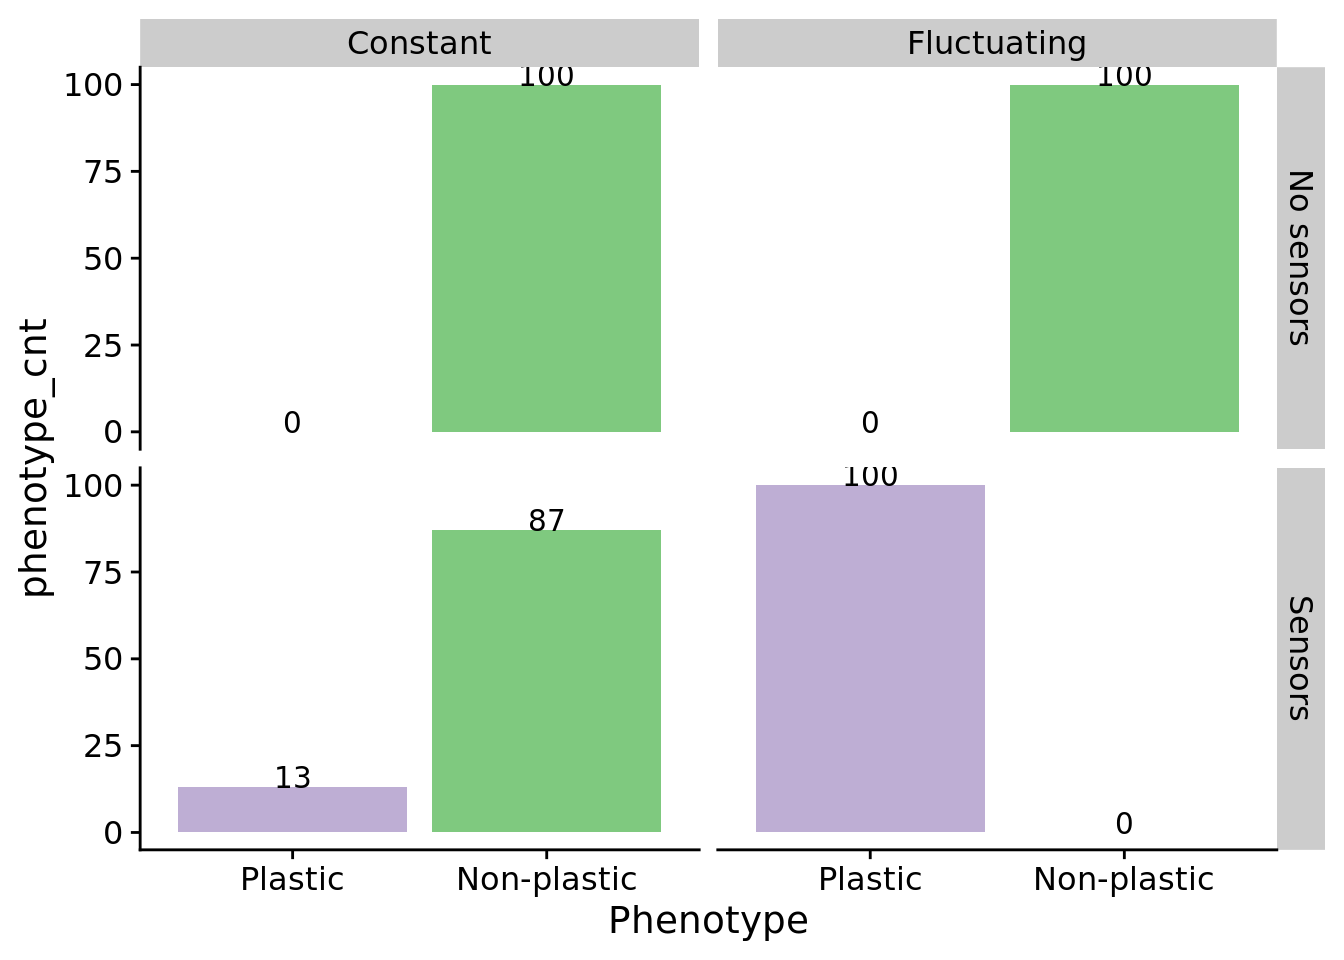
\includegraphics{supplemental-material_files/figure-latex/unnamed-chunk-5-1.pdf}

Indeed, we do not observe the evolution of phenotypic plasticity in any replicates in which digital organisms do not have access to sensory instructions.
We do observe the evolution of plasticity (not necessarily adaptive plasticity) in both constant and fluctuating environments where sensors are enabled.

To what extent is the observed phenotypic plasticity adaptive?

\begin{Shaded}
\begin{Highlighting}[]
\KeywordTok{ggplot}\NormalTok{(}\KeywordTok{filter}\NormalTok{(observed_plasticity, environment}\OperatorTok{==}\StringTok{"Fluctuating"} \OperatorTok{&}\StringTok{ }\NormalTok{sensors }\OperatorTok{==}\StringTok{ "Sensors"} \OperatorTok{&}\StringTok{ }\NormalTok{phenotype }\OperatorTok\StringTok{ }\KeywordTok{c}\NormalTok{(}\StringTok{"plastic"}\NormalTok{, }\StringTok{"plastic_adaptive"}\NormalTok{, }\StringTok{"plastic_optimal"}\NormalTok{, }\StringTok{"plastic_nonadaptive"}\NormalTok{)), }\KeywordTok{aes}\NormalTok{(}\DataTypeTok{x=}\NormalTok{phenotype, }\DataTypeTok{y=}\NormalTok{phenotype_cnt, }\DataTypeTok{fill=}\NormalTok{phenotype)) }\OperatorTok{+}
\StringTok{  }\KeywordTok{geom_bar}\NormalTok{(}
    \DataTypeTok{stat=}\StringTok{"identity"}\NormalTok{,}
    \DataTypeTok{position=}\KeywordTok{position_dodge}\NormalTok{(}\FloatTok{0.9}\NormalTok{)}
\NormalTok{  ) }\OperatorTok{+}
\StringTok{  }\KeywordTok{geom_text}\NormalTok{(}
    \DataTypeTok{stat=}\StringTok{"identity"}\NormalTok{,}
    \DataTypeTok{mapping=}\KeywordTok{aes}\NormalTok{(}\DataTypeTok{label=}\NormalTok{phenotype_cnt),}
    \DataTypeTok{vjust=}\FloatTok{0.05}
\NormalTok{  ) }\OperatorTok{+}
\StringTok{  }\KeywordTok{scale_fill_brewer}\NormalTok{(}\DataTypeTok{palette=}\StringTok{"Accent"}\NormalTok{) }\OperatorTok{+}
\StringTok{  }\KeywordTok{scale_x_discrete}\NormalTok{(}
    \DataTypeTok{name=}\StringTok{"Phenotype"}\NormalTok{,}
    \DataTypeTok{limits=}\KeywordTok{c}\NormalTok{(}\StringTok{"plastic"}\NormalTok{,  }\StringTok{"plastic_adaptive"}\NormalTok{, }\StringTok{"plastic_optimal"}\NormalTok{, }\StringTok{"plastic_nonadaptive"}\NormalTok{),}
    \DataTypeTok{labels=}\KeywordTok{c}\NormalTok{(}\StringTok{"Total plastic"}\NormalTok{, }\StringTok{"Adaptive plasticity"}\NormalTok{, }\StringTok{"Optimal plasticity"}\NormalTok{, }\StringTok{"Non-adaptive plasticity"}\NormalTok{)}
\NormalTok{  ) }\OperatorTok{+}
\StringTok{  }\KeywordTok{facet_grid}\NormalTok{(sensors}\OperatorTok{~}\NormalTok{environment) }\OperatorTok{+}
\StringTok{  }\KeywordTok{theme}\NormalTok{(}
    \DataTypeTok{legend.position=}\StringTok{"none"}
\NormalTok{  )}
\end{Highlighting}
\end{Shaded}

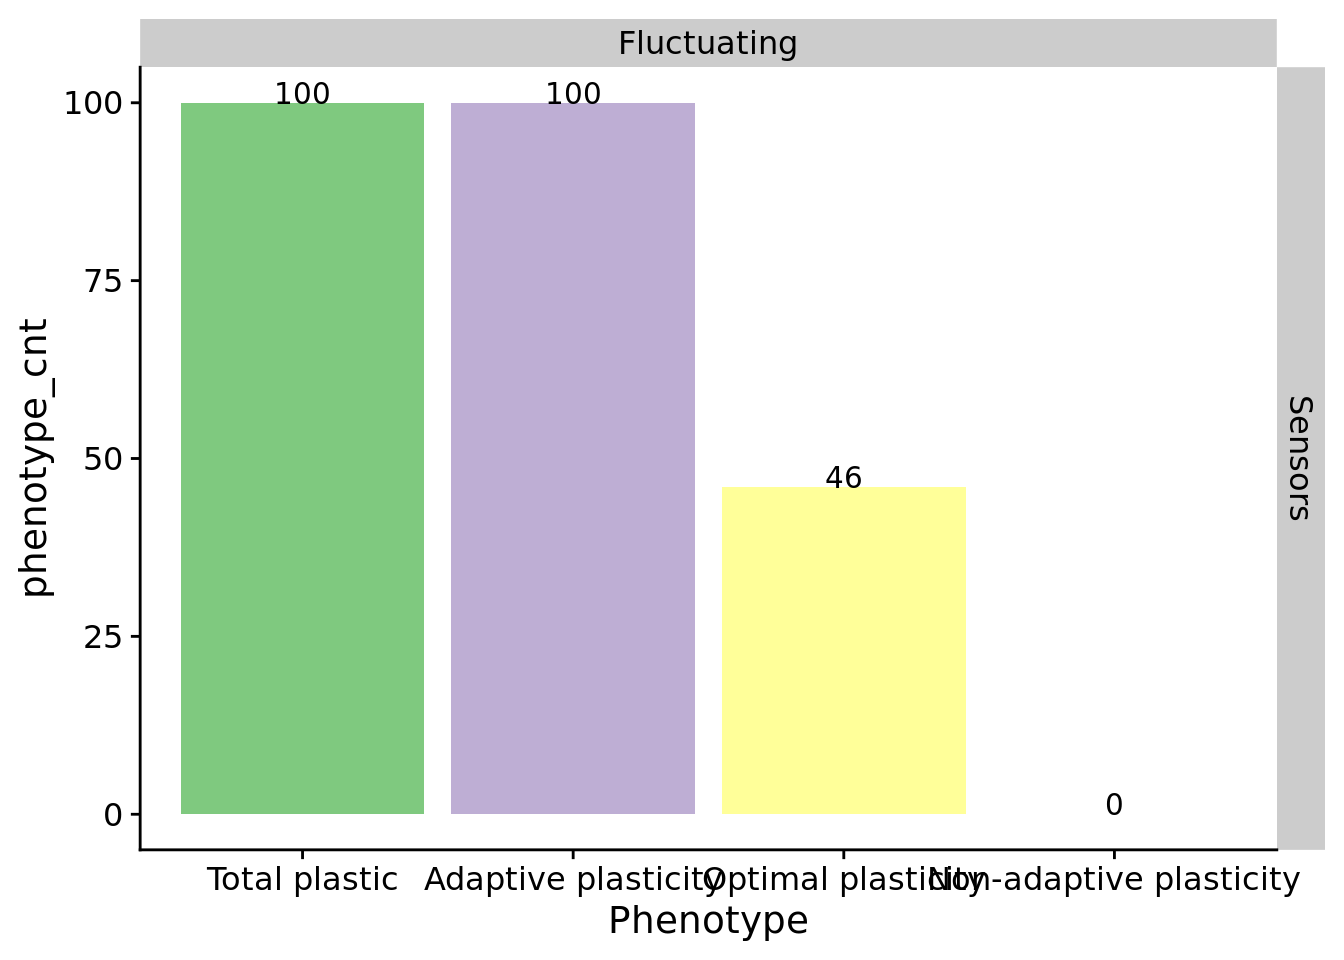
\includegraphics{supplemental-material_files/figure-latex/unnamed-chunk-6-1.pdf}

\hypertarget{evolutionary-change}{%
\chapter{Evolutionary change}\label{evolutionary-change}}

The effect of adaptive phenotypic plasticity on evolutionary change.

\hypertarget{overview-1}{%
\section{Overview}\label{overview-1}}

\begin{Shaded}
\begin{Highlighting}[]
\NormalTok{total_updates <-}\StringTok{ }\DecValTok{200000}
\NormalTok{replicates <-}\StringTok{ }\DecValTok{100}
\NormalTok{alpha <-}\StringTok{ }\FloatTok{0.05}

\NormalTok{all_traits <-}\StringTok{ }\KeywordTok{c}\NormalTok{(}\StringTok{"not"}\NormalTok{,}\StringTok{"nand"}\NormalTok{,}\StringTok{"and"}\NormalTok{,}\StringTok{"ornot"}\NormalTok{,}\StringTok{"or"}\NormalTok{,}\StringTok{"andnot"}\NormalTok{)}
\NormalTok{traits_set_a <-}\StringTok{ }\KeywordTok{c}\NormalTok{(}\StringTok{"not"}\NormalTok{, }\StringTok{"and"}\NormalTok{, }\StringTok{"or"}\NormalTok{)}
\NormalTok{traits_set_b <-}\StringTok{ }\KeywordTok{c}\NormalTok{(}\StringTok{"nand"}\NormalTok{, }\StringTok{"ornot"}\NormalTok{, }\StringTok{"andnot"}\NormalTok{)}

\CommentTok{# Relative location of data.}
\NormalTok{working_directory <-}\StringTok{ "experiments/2021-02-08-evo-dynamics/analysis/"} \CommentTok{# << For bookdown}
\CommentTok{# working_directory <- "./"                                              # << For local analysis}
\end{Highlighting}
\end{Shaded}

\hypertarget{analysis-dependencies-1}{%
\section{Analysis dependencies}\label{analysis-dependencies-1}}

Load all required R libraries.

\begin{Shaded}
\begin{Highlighting}[]
\KeywordTok{library}\NormalTok{(ggplot2)}
\KeywordTok{library}\NormalTok{(rstatix)}
\KeywordTok{library}\NormalTok{(ggsignif)}
\KeywordTok{library}\NormalTok{(scales)}
\KeywordTok{library}\NormalTok{(tidyverse)}
\KeywordTok{library}\NormalTok{(cowplot)}
\KeywordTok{library}\NormalTok{(RColorBrewer)}
\KeywordTok{library}\NormalTok{(Hmisc)}
\KeywordTok{library}\NormalTok{(boot)}
\KeywordTok{source}\NormalTok{(}\StringTok{"https://gist.githubusercontent.com/benmarwick/2a1bb0133ff568cbe28d/raw/fb53bd97121f7f9ce947837ef1a4c65a73bffb3f/geom_flat_violin.R"}\NormalTok{)}
\end{Highlighting}
\end{Shaded}

These analyses were conducted/knitted with the following computing environment:

\begin{Shaded}
\begin{Highlighting}[]
\KeywordTok{print}\NormalTok{(version)}
\end{Highlighting}
\end{Shaded}

\begin{verbatim}
##                _                           
## platform       x86_64-pc-linux-gnu         
## arch           x86_64                      
## os             linux-gnu                   
## system         x86_64, linux-gnu           
## status                                     
## major          4                           
## minor          1.3                         
## year           2022                        
## month          03                          
## day            10                          
## svn rev        81868                       
## language       R                           
## version.string R version 4.1.3 (2022-03-10)
## nickname       One Push-Up
\end{verbatim}

\hypertarget{setup-1}{%
\section{Setup}\label{setup-1}}

\begin{Shaded}
\begin{Highlighting}[]
\NormalTok{summary_data_loc <-}\StringTok{ }\KeywordTok{paste0}\NormalTok{(working_directory, }\StringTok{"data/aggregate.csv"}\NormalTok{)}
\NormalTok{summary_data <-}\StringTok{ }\KeywordTok{read.csv}\NormalTok{(summary_data_loc, }\DataTypeTok{na.strings=}\StringTok{"NONE"}\NormalTok{)}

\NormalTok{summary_data}\OperatorTok{$}\NormalTok{DISABLE_REACTION_SENSORS <-}\StringTok{ }\KeywordTok{as.factor}\NormalTok{(summary_data}\OperatorTok{$}\NormalTok{DISABLE_REACTION_SENSORS)}
\NormalTok{summary_data}\OperatorTok{$}\NormalTok{chg_env <-}\StringTok{ }\NormalTok{summary_data}\OperatorTok{$}\NormalTok{chg_env }\OperatorTok{==}\StringTok{ "True"}
\NormalTok{summary_data}\OperatorTok{$}\NormalTok{dominant_plastic_odd_even <-}\StringTok{ }\KeywordTok{as.factor}\NormalTok{(summary_data}\OperatorTok{$}\NormalTok{dominant_plastic_odd_even)}
\NormalTok{summary_data}\OperatorTok{$}\NormalTok{sensors <-}\StringTok{ }\NormalTok{summary_data}\OperatorTok{$}\NormalTok{DISABLE_REACTION_SENSORS }\OperatorTok{==}\StringTok{ "0"}
\NormalTok{summary_data}\OperatorTok{$}\NormalTok{is_plastic <-}\StringTok{ }\NormalTok{summary_data}\OperatorTok{$}\NormalTok{dominant_plastic_odd_even }\OperatorTok{==}\StringTok{ "True"}

\NormalTok{env_label_fun <-}\StringTok{ }\ControlFlowTok{function}\NormalTok{(chg_env) \{}
  \ControlFlowTok{if}\NormalTok{ (chg_env) \{}
    \KeywordTok{return}\NormalTok{(}\StringTok{"Fluctuating"}\NormalTok{)}
\NormalTok{  \} }\ControlFlowTok{else}\NormalTok{ \{}
    \KeywordTok{return}\NormalTok{(}\StringTok{"Constant"}\NormalTok{)}
\NormalTok{  \}}
\NormalTok{\}}

\NormalTok{sensors_label_fun <-}\StringTok{ }\ControlFlowTok{function}\NormalTok{(has_sensors) \{}
  \ControlFlowTok{if}\NormalTok{ (has_sensors) \{}
    \KeywordTok{return}\NormalTok{(}\StringTok{"Sensors"}\NormalTok{)}
\NormalTok{  \} }\ControlFlowTok{else}\NormalTok{ \{}
    \KeywordTok{return}\NormalTok{(}\StringTok{"No sensors"}\NormalTok{)}
\NormalTok{  \}}
\NormalTok{\}}

\CommentTok{# note that this labeler makes assumptions about how we set up our experiment}
\NormalTok{condition_label_fun <-}\StringTok{ }\ControlFlowTok{function}\NormalTok{(has_sensors, env_chg) \{}
  \ControlFlowTok{if}\NormalTok{ (has_sensors }\OperatorTok{&&}\StringTok{ }\NormalTok{env_chg) \{}
    \KeywordTok{return}\NormalTok{(}\StringTok{"PLASTIC"}\NormalTok{)}
\NormalTok{  \} }\ControlFlowTok{else} \ControlFlowTok{if}\NormalTok{ (env_chg) \{}
    \KeywordTok{return}\NormalTok{(}\StringTok{"NON-PLASTIC"}\NormalTok{)}
\NormalTok{  \} }\ControlFlowTok{else}\NormalTok{ \{}
    \KeywordTok{return}\NormalTok{(}\StringTok{"STATIC"}\NormalTok{)}
\NormalTok{  \}}
\NormalTok{\}}

\NormalTok{summary_data}\OperatorTok{$}\NormalTok{env_label <-}\StringTok{ }\KeywordTok{mapply}\NormalTok{(}
\NormalTok{  env_label_fun,}
\NormalTok{  summary_data}\OperatorTok{$}\NormalTok{chg_env}
\NormalTok{)}
\NormalTok{summary_data}\OperatorTok{$}\NormalTok{sensors_label <-}\StringTok{ }\KeywordTok{mapply}\NormalTok{(}
\NormalTok{  sensors_label_fun,}
\NormalTok{  summary_data}\OperatorTok{$}\NormalTok{sensors}
\NormalTok{)}
\NormalTok{summary_data}\OperatorTok{$}\NormalTok{condition <-}\StringTok{ }\KeywordTok{mapply}\NormalTok{(}
\NormalTok{  condition_label_fun,}
\NormalTok{  summary_data}\OperatorTok{$}\NormalTok{sensors,}
\NormalTok{  summary_data}\OperatorTok{$}\NormalTok{chg_env}
\NormalTok{)}

\NormalTok{condition_order =}\StringTok{ }\KeywordTok{c}\NormalTok{(}
  \StringTok{"STATIC"}\NormalTok{,}
  \StringTok{"NON-PLASTIC"}\NormalTok{,}
  \StringTok{"PLASTIC"}
\NormalTok{)}
\NormalTok{pairwise_comparisons <-}\StringTok{ }\KeywordTok{list}\NormalTok{(}
  \KeywordTok{c}\NormalTok{(}\StringTok{"STATIC"}\NormalTok{, }\StringTok{"NON-PLASTIC"}\NormalTok{),}
  \KeywordTok{c}\NormalTok{(}\StringTok{"STATIC"}\NormalTok{, }\StringTok{"PLASTIC"}\NormalTok{),}
  \KeywordTok{c}\NormalTok{(}\StringTok{"PLASTIC"}\NormalTok{, }\StringTok{"NON-PLASTIC"}\NormalTok{)}
\NormalTok{)}

\NormalTok{p_label <-}\StringTok{ }\ControlFlowTok{function}\NormalTok{(p_value) \{}
\NormalTok{  threshold =}\StringTok{ }\FloatTok{0.0001}
  \ControlFlowTok{if}\NormalTok{ (p_value }\OperatorTok{<}\StringTok{ }\NormalTok{threshold) \{}
    \KeywordTok{return}\NormalTok{(}\KeywordTok{paste0}\NormalTok{(}\StringTok{"p < "}\NormalTok{, threshold))}
\NormalTok{  \} }\ControlFlowTok{else}\NormalTok{ \{}
    \KeywordTok{return}\NormalTok{(}\KeywordTok{paste0}\NormalTok{(}\StringTok{"p = "}\NormalTok{, p_value))}
\NormalTok{  \}}
\NormalTok{\}}

\CommentTok{# *really* inefficient way to identify outliers}
\NormalTok{is_outlier <-}\StringTok{ }\ControlFlowTok{function}\NormalTok{(value, cond, data, column) \{}
\NormalTok{  cond_data <-}\StringTok{ }\KeywordTok{filter}\NormalTok{(data, condition}\OperatorTok{==}\NormalTok{cond)}
\NormalTok{  q1 <-}\StringTok{ }\KeywordTok{summary}\NormalTok{(cond_data[,column])[[}\StringTok{"1st Qu."}\NormalTok{]]}
\NormalTok{  q3 <-}\StringTok{ }\KeywordTok{summary}\NormalTok{(cond_data[,column])[[}\StringTok{"3rd Qu."}\NormalTok{]]}
\NormalTok{  H <-}\StringTok{ }\FloatTok{1.5} \OperatorTok{*}\StringTok{ }\KeywordTok{IQR}\NormalTok{(cond_data[,column])}
  \KeywordTok{return}\NormalTok{( (value }\OperatorTok{<}\StringTok{ }\NormalTok{(q1}\OperatorTok{-}\NormalTok{H)) }\OperatorTok{||}\StringTok{ }\NormalTok{(value }\OperatorTok{>}\StringTok{ }\NormalTok{(q3}\OperatorTok{+}\NormalTok{H)) )}
\NormalTok{\}}

\CommentTok{####### misc #######}
\CommentTok{# Configure our default graphing theme}
\KeywordTok{theme_set}\NormalTok{(}\KeywordTok{theme_cowplot}\NormalTok{())}
\CommentTok{# Palette}
\NormalTok{cb_palette <-}\StringTok{ "Paired"}
\CommentTok{# Create a directory to store plots}
\KeywordTok{dir.create}\NormalTok{(}\KeywordTok{paste0}\NormalTok{(working_directory, }\StringTok{"plots"}\NormalTok{), }\DataTypeTok{showWarnings=}\OtherTok{FALSE}\NormalTok{)}
\CommentTok{# Define sample mean function}
\NormalTok{samplemean <-}\StringTok{ }\ControlFlowTok{function}\NormalTok{(x, d) \{}
  \KeywordTok{return}\NormalTok{(}\KeywordTok{mean}\NormalTok{(x[d]))}
\NormalTok{\}}
\end{Highlighting}
\end{Shaded}

\hypertarget{the-evolution-of-phenotypic-plasticity}{%
\section{The evolution of phenotypic plasticity}\label{the-evolution-of-phenotypic-plasticity}}

For sensor-enabled populations in fluctuating environments, we only transfered populations containing an optimally plastic genotype to phase-two.

\begin{Shaded}
\begin{Highlighting}[]
\NormalTok{summary_data_grouped =}\StringTok{ }\NormalTok{dplyr}\OperatorTok{::}\KeywordTok{group_by}\NormalTok{(summary_data, condition)}
\NormalTok{summary_data_group_counts =}\StringTok{ }\NormalTok{dplyr}\OperatorTok{::}\KeywordTok{summarize}\NormalTok{(summary_data_grouped, }\DataTypeTok{n=}\NormalTok{dplyr}\OperatorTok{::}\KeywordTok{n}\NormalTok{())}

\KeywordTok{ggplot}\NormalTok{(summary_data_group_counts, }\KeywordTok{aes}\NormalTok{(}\DataTypeTok{x=}\NormalTok{condition, }\DataTypeTok{y=}\NormalTok{n, }\DataTypeTok{fill=}\NormalTok{condition)) }\OperatorTok{+}
\StringTok{  }\KeywordTok{geom_col}\NormalTok{(}\DataTypeTok{position=}\KeywordTok{position_dodge}\NormalTok{(}\FloatTok{0.9}\NormalTok{)) }\OperatorTok{+}
\StringTok{  }\KeywordTok{geom_text}\NormalTok{(}\KeywordTok{aes}\NormalTok{(}\DataTypeTok{label=}\NormalTok{n, }\DataTypeTok{y=}\NormalTok{n}\OperatorTok{+}\DecValTok{2}\NormalTok{)) }\OperatorTok{+}
\StringTok{  }\KeywordTok{scale_x_discrete}\NormalTok{(}
    \DataTypeTok{name=}\StringTok{"Condition"}\NormalTok{,}
    \DataTypeTok{limits=}\NormalTok{condition_order}
\NormalTok{  ) }\OperatorTok{+}
\StringTok{  }\KeywordTok{scale_fill_brewer}\NormalTok{(}
    \DataTypeTok{palette=}\NormalTok{cb_palette}
\NormalTok{  ) }\OperatorTok{+}
\StringTok{  }\KeywordTok{scale_color_brewer}\NormalTok{(}
    \DataTypeTok{palette=}\NormalTok{cb_palette}
\NormalTok{  ) }\OperatorTok{+}
\StringTok{  }\KeywordTok{ylab}\NormalTok{(}\StringTok{"Number of replicates transferred to phase two"}\NormalTok{) }\OperatorTok{+}
\StringTok{  }\KeywordTok{theme}\NormalTok{(}
    \DataTypeTok{legend.position=}\StringTok{"none"}
\NormalTok{  )}
\end{Highlighting}
\end{Shaded}

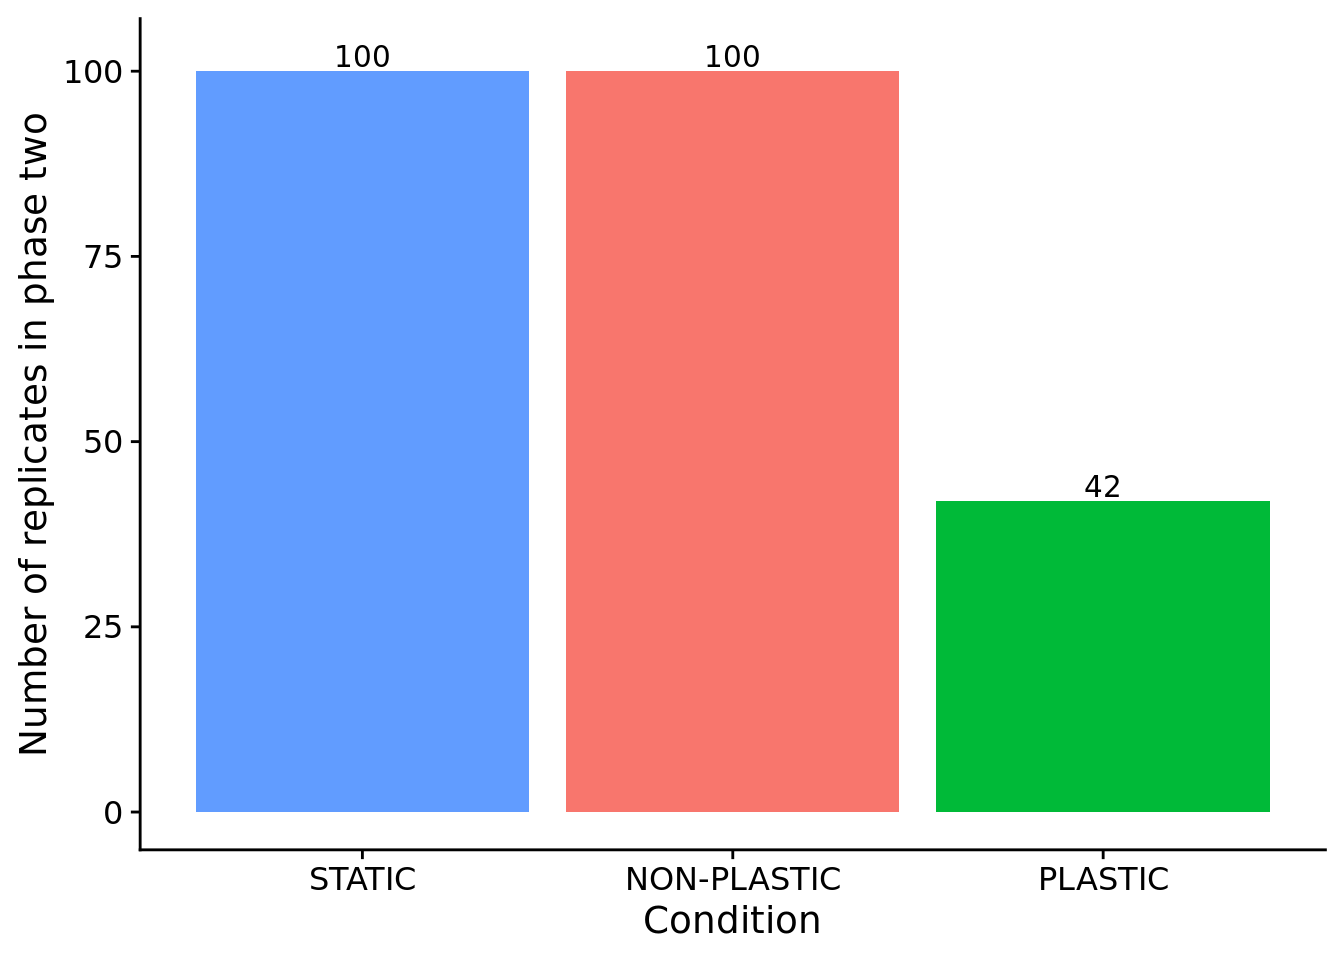
\includegraphics{supplemental-material_files/figure-latex/unnamed-chunk-11-1.pdf}

We can confirm our expectation that the dominant genotypes in non-plastic conditions are not phenotypically plastic.

\begin{Shaded}
\begin{Highlighting}[]
\NormalTok{summary_data_grouped =}\StringTok{ }\NormalTok{dplyr}\OperatorTok{::}\KeywordTok{group_by}\NormalTok{(summary_data, condition, is_plastic)}
\NormalTok{summary_data_group_counts =}\StringTok{ }\NormalTok{dplyr}\OperatorTok{::}\KeywordTok{summarize}\NormalTok{(summary_data_grouped, }\DataTypeTok{n=}\NormalTok{dplyr}\OperatorTok{::}\KeywordTok{n}\NormalTok{())}
\KeywordTok{ggplot}\NormalTok{(}\KeywordTok{filter}\NormalTok{(summary_data_group_counts, is_plastic), }\KeywordTok{aes}\NormalTok{(}\DataTypeTok{x=}\NormalTok{condition, }\DataTypeTok{y=}\NormalTok{n, }\DataTypeTok{fill=}\NormalTok{condition)) }\OperatorTok{+}
\StringTok{  }\KeywordTok{geom_col}\NormalTok{(}
    \DataTypeTok{position=}\KeywordTok{position_dodge}\NormalTok{(}\FloatTok{0.9}\NormalTok{)}
\NormalTok{  ) }\OperatorTok{+}
\StringTok{  }\KeywordTok{scale_x_discrete}\NormalTok{(}
    \DataTypeTok{name=}\StringTok{"Condition"}\NormalTok{,}
    \DataTypeTok{limits=}\NormalTok{condition_order}
\NormalTok{  ) }\OperatorTok{+}
\StringTok{  }\KeywordTok{scale_fill_brewer}\NormalTok{(}
    \DataTypeTok{palette=}\NormalTok{cb_palette}
\NormalTok{  ) }\OperatorTok{+}
\StringTok{  }\KeywordTok{scale_color_brewer}\NormalTok{(}
    \DataTypeTok{palette=}\NormalTok{cb_palette}
\NormalTok{  ) }\OperatorTok{+}
\StringTok{  }\KeywordTok{geom_text}\NormalTok{(}\KeywordTok{aes}\NormalTok{(}\DataTypeTok{label=}\NormalTok{n, }\DataTypeTok{y=}\NormalTok{n}\OperatorTok{+}\DecValTok{1}\NormalTok{)) }\OperatorTok{+}
\StringTok{  }\KeywordTok{ylab}\NormalTok{(}\StringTok{"Number of plastic replicates"}\NormalTok{) }\OperatorTok{+}
\StringTok{  }\KeywordTok{ylim}\NormalTok{(}\DecValTok{0}\NormalTok{, }\DecValTok{100}\NormalTok{) }\OperatorTok{+}
\StringTok{  }\KeywordTok{theme}\NormalTok{(}
    \DataTypeTok{legend.position=}\StringTok{"none"}
\NormalTok{  )}
\end{Highlighting}
\end{Shaded}

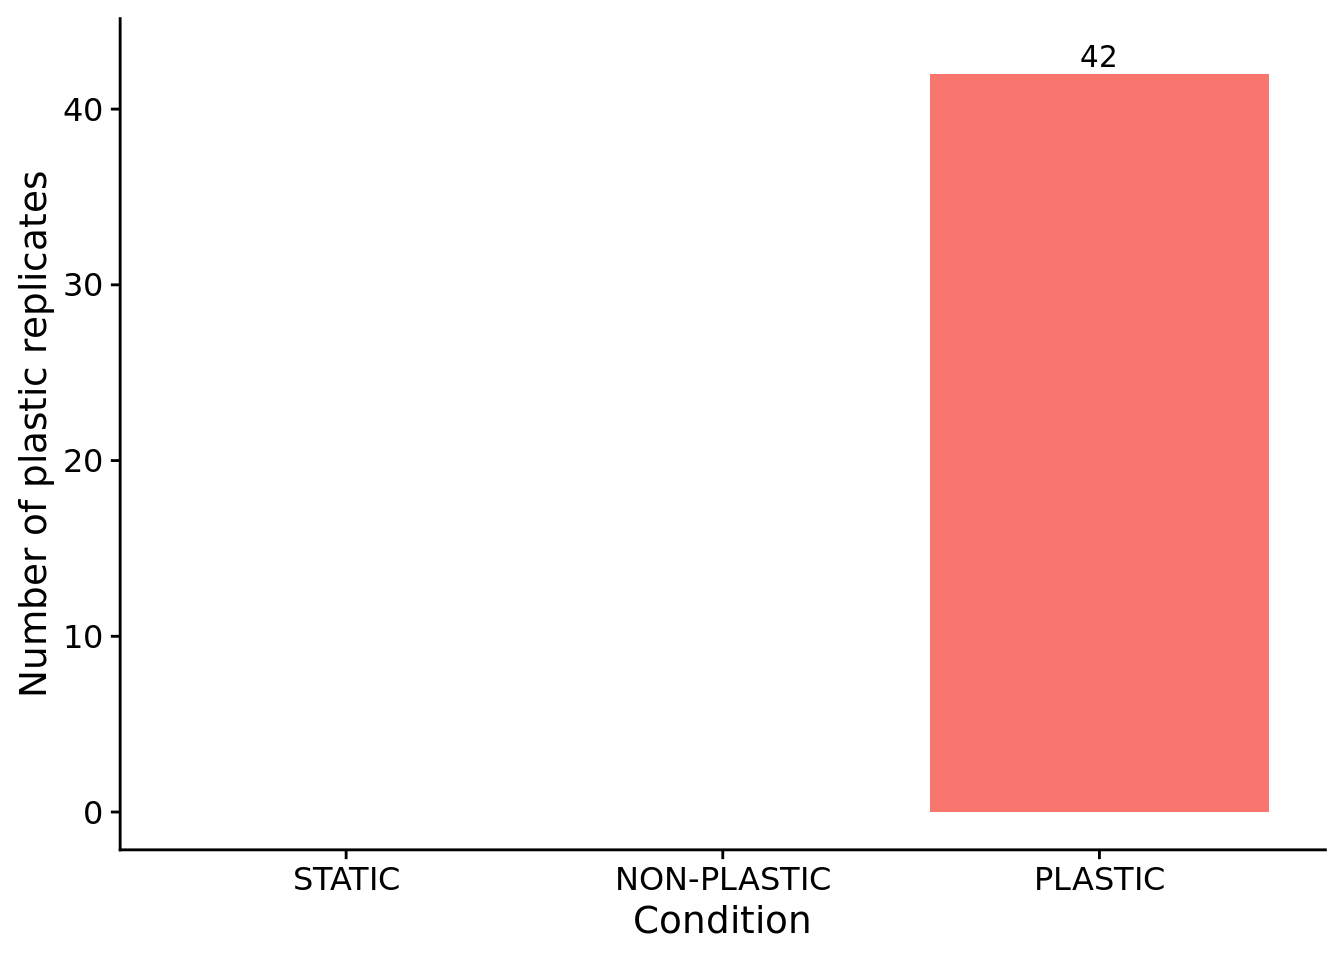
\includegraphics{supplemental-material_files/figure-latex/unnamed-chunk-12-1.pdf}

\hypertarget{average-generation}{%
\section{Average generation}\label{average-generation}}

How many generations elapsed in each of of our treatments?

\begin{Shaded}
\begin{Highlighting}[]
\KeywordTok{ggplot}\NormalTok{(summary_data, }\KeywordTok{aes}\NormalTok{(}\DataTypeTok{x=}\NormalTok{condition, }\DataTypeTok{y=}\NormalTok{time_average_generation, }\DataTypeTok{fill=}\NormalTok{condition)) }\OperatorTok{+}
\StringTok{  }\KeywordTok{geom_flat_violin}\NormalTok{(}
    \DataTypeTok{position =} \KeywordTok{position_nudge}\NormalTok{(}\DataTypeTok{x =} \FloatTok{.2}\NormalTok{, }\DataTypeTok{y =} \DecValTok{0}\NormalTok{),}
    \DataTypeTok{alpha =} \FloatTok{.8}
\NormalTok{  ) }\OperatorTok{+}
\StringTok{  }\KeywordTok{geom_point}\NormalTok{(}
    \DataTypeTok{mapping=}\KeywordTok{aes}\NormalTok{(}\DataTypeTok{color=}\NormalTok{condition),}
    \DataTypeTok{position =} \KeywordTok{position_jitter}\NormalTok{(}\DataTypeTok{width =} \FloatTok{.15}\NormalTok{),}
    \DataTypeTok{size =} \FloatTok{.5}\NormalTok{,}
    \DataTypeTok{alpha =} \FloatTok{0.8}
\NormalTok{  ) }\OperatorTok{+}
\StringTok{  }\KeywordTok{geom_boxplot}\NormalTok{(}
    \DataTypeTok{width =} \FloatTok{.1}\NormalTok{,}
    \DataTypeTok{outlier.shape =} \OtherTok{NA}\NormalTok{,}
    \DataTypeTok{alpha =} \FloatTok{0.5}
\NormalTok{  ) }\OperatorTok{+}
\StringTok{  }\KeywordTok{scale_x_discrete}\NormalTok{(}
    \DataTypeTok{name=}\StringTok{"Condition"}\NormalTok{,}
    \DataTypeTok{limits=}\NormalTok{condition_order}
\NormalTok{  ) }\OperatorTok{+}
\StringTok{  }\KeywordTok{scale_fill_brewer}\NormalTok{(}
    \DataTypeTok{palette=}\NormalTok{cb_palette}
\NormalTok{  ) }\OperatorTok{+}
\StringTok{  }\KeywordTok{scale_color_brewer}\NormalTok{(}
    \DataTypeTok{palette=}\NormalTok{cb_palette}
\NormalTok{  ) }\OperatorTok{+}
\StringTok{  }\CommentTok{# coord_flip() +}
\StringTok{  }\KeywordTok{ylab}\NormalTok{(}\StringTok{"average generation"}\NormalTok{) }\OperatorTok{+}
\StringTok{  }\KeywordTok{theme}\NormalTok{(}
    \DataTypeTok{legend.position=}\StringTok{"none"}
\NormalTok{  )}
\end{Highlighting}
\end{Shaded}

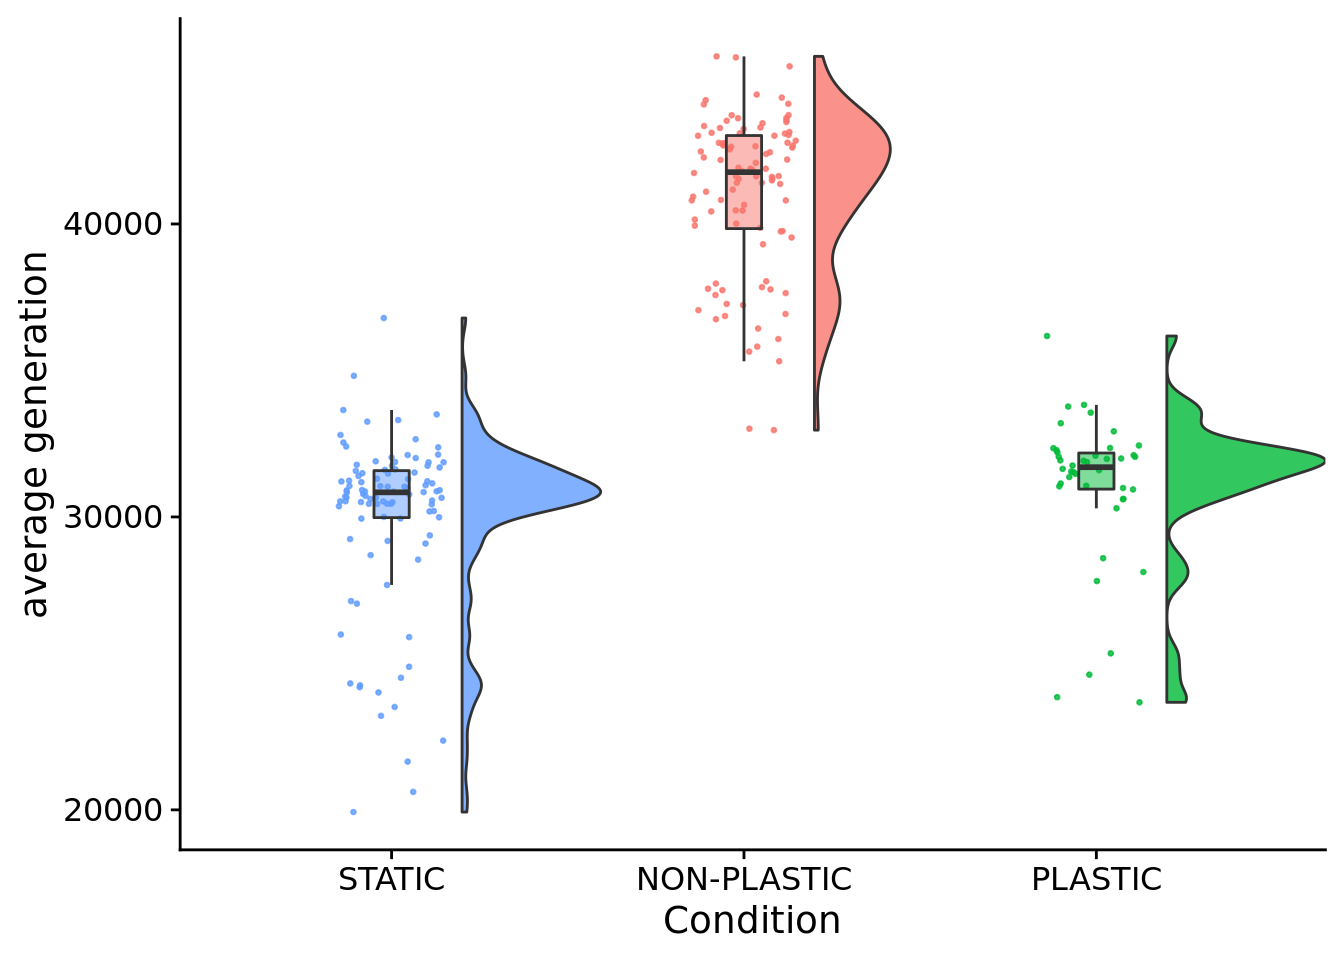
\includegraphics{supplemental-material_files/figure-latex/unnamed-chunk-13-1.pdf}

\begin{Shaded}
\begin{Highlighting}[]
\KeywordTok{ggsave}\NormalTok{(}\KeywordTok{paste0}\NormalTok{(working_directory, }\StringTok{"plots/"}\NormalTok{, }\StringTok{"average-generation.png"}\NormalTok{))}
\end{Highlighting}
\end{Shaded}

\begin{verbatim}
## Saving 6.5 x 4.5 in image
\end{verbatim}

\begin{Shaded}
\begin{Highlighting}[]
\KeywordTok{kruskal.test}\NormalTok{(}
  \DataTypeTok{formula=}\NormalTok{time_average_generation}\OperatorTok{~}\NormalTok{condition,}
  \DataTypeTok{data=}\NormalTok{summary_data}
\NormalTok{)}
\end{Highlighting}
\end{Shaded}

\begin{verbatim}
## 
##  Kruskal-Wallis rank sum test
## 
## data:  time_average_generation by condition
## Kruskal-Wallis chi-squared = 177.33, df = 2, p-value < 2.2e-16
\end{verbatim}

\begin{Shaded}
\begin{Highlighting}[]
\KeywordTok{pairwise.wilcox.test}\NormalTok{(}
  \DataTypeTok{x=}\NormalTok{summary_data}\OperatorTok{$}\NormalTok{time_average_generation,}
  \DataTypeTok{g=}\NormalTok{summary_data}\OperatorTok{$}\NormalTok{condition,}
  \DataTypeTok{p.adjust.method=}\StringTok{"bonferroni"}\NormalTok{,}
\NormalTok{)}
\end{Highlighting}
\end{Shaded}

\begin{verbatim}
## 
##  Pairwise comparisons using Wilcoxon rank sum test with continuity correction 
## 
## data:  summary_data$time_average_generation and summary_data$condition 
## 
##         NON-PLASTIC PLASTIC
## PLASTIC <2e-16      -      
## STATIC  <2e-16      0.004  
## 
## P value adjustment method: bonferroni
\end{verbatim}

\begin{Shaded}
\begin{Highlighting}[]
\KeywordTok{paste}\NormalTok{(}
  \DataTypeTok{sep=}\StringTok{"; "}\NormalTok{,}
  \KeywordTok{paste0}\NormalTok{(}
    \StringTok{"PLASTIC median: "}\NormalTok{,}
    \KeywordTok{median}\NormalTok{(}\KeywordTok{filter}\NormalTok{(summary_data, condition}\OperatorTok{==}\StringTok{"PLASTIC"}\NormalTok{)}\OperatorTok{$}\NormalTok{time_average_generation)}
\NormalTok{  ),}
  \KeywordTok{paste0}\NormalTok{(}
    \StringTok{"STATIC median: "}\NormalTok{,}
    \KeywordTok{median}\NormalTok{(}\KeywordTok{filter}\NormalTok{(summary_data, condition}\OperatorTok{==}\StringTok{"STATIC"}\NormalTok{)}\OperatorTok{$}\NormalTok{time_average_generation)}
\NormalTok{  ),}
  \KeywordTok{paste0}\NormalTok{(}
    \StringTok{"NON-PLASTIC median: "}\NormalTok{,}
    \KeywordTok{median}\NormalTok{(}\KeywordTok{filter}\NormalTok{(summary_data, condition}\OperatorTok{==}\StringTok{"NON-PLASTIC"}\NormalTok{)}\OperatorTok{$}\NormalTok{time_average_generation)}
\NormalTok{  )}
\NormalTok{)}
\end{Highlighting}
\end{Shaded}

\begin{verbatim}
## [1] "PLASTIC median: 31697.65; STATIC median: 30839.75; NON-PLASTIC median: 41768.65"
\end{verbatim}

\begin{Shaded}
\begin{Highlighting}[]
\KeywordTok{print}\NormalTok{(}\StringTok{"Wilcox rank sum test statistics:"}\NormalTok{)}
\end{Highlighting}
\end{Shaded}

\begin{verbatim}
## [1] "Wilcox rank sum test statistics:"
\end{verbatim}

\begin{Shaded}
\begin{Highlighting}[]
\ControlFlowTok{for}\NormalTok{ (pair }\ControlFlowTok{in}\NormalTok{ pairwise_comparisons) \{}
\NormalTok{  pair_data <-}\StringTok{ }\KeywordTok{filter}\NormalTok{(summary_data, condition }\OperatorTok\StringTok{ }\NormalTok{pair)}
\NormalTok{  pair_data}\OperatorTok{$}\NormalTok{condition <-}\StringTok{ }\KeywordTok{as.factor}\NormalTok{(pair_data}\OperatorTok{$}\NormalTok{condition)}
\NormalTok{  wt <-}\StringTok{ }\KeywordTok{wilcox.test}\NormalTok{(}
    \DataTypeTok{formula=}\NormalTok{time_average_generation}\OperatorTok{~}\NormalTok{condition,}
    \DataTypeTok{data=}\NormalTok{pair_data,}
    \DataTypeTok{exact=}\OtherTok{FALSE}\NormalTok{,}
    \DataTypeTok{paired=}\OtherTok{FALSE}
\NormalTok{  )}
  \KeywordTok{print}\NormalTok{(}\KeywordTok{paste0}\NormalTok{(pair[}\DecValTok{1}\NormalTok{], }\StringTok{"<-->"}\NormalTok{, pair[}\DecValTok{2}\NormalTok{], }\StringTok{": W="}\NormalTok{,wt}\OperatorTok{$}\NormalTok{statistic))}
\NormalTok{\}}
\end{Highlighting}
\end{Shaded}

\begin{verbatim}
## [1] "STATIC<-->NON-PLASTIC: W=9982"
## [1] "STATIC<-->PLASTIC: W=2818"
## [1] "PLASTIC<-->NON-PLASTIC: W=4186"
\end{verbatim}

\begin{Shaded}
\begin{Highlighting}[]
\NormalTok{summary_data }\OperatorTok
\StringTok{  }\KeywordTok{group_by}\NormalTok{(condition) }\OperatorTok
\StringTok{  }\KeywordTok{summarise}\NormalTok{(}\DataTypeTok{mean=}\KeywordTok{mean}\NormalTok{(time_average_generation),}\DataTypeTok{sd=}\KeywordTok{sd}\NormalTok{(time_average_generation))}
\end{Highlighting}
\end{Shaded}

\begin{verbatim}
## # A tibble: 3 x 3
##   condition     mean    sd
##   <chr>        <dbl> <dbl>
## 1 NON-PLASTIC 41090. 2702.
## 2 PLASTIC     31016. 2615.
## 3 STATIC      30002. 3011.
\end{verbatim}

\hypertarget{coalescence-event-count}{%
\section{Coalescence event count}\label{coalescence-event-count}}

The number of times the most recent common ancestor changes gives us the number of selective sweeps that occur during the experiment.

\begin{Shaded}
\begin{Highlighting}[]
\CommentTok{# Compute manual labels for geom_signif}
\NormalTok{stat.test <-}\StringTok{ }\NormalTok{summary_data }\OperatorTok
\StringTok{  }\KeywordTok{wilcox_test}\NormalTok{(phylo_mrca_changes }\OperatorTok{~}\StringTok{ }\NormalTok{condition) }\OperatorTok
\StringTok{  }\KeywordTok{adjust_pvalue}\NormalTok{(}\DataTypeTok{method =} \StringTok{"bonferroni"}\NormalTok{) }\OperatorTok
\StringTok{  }\KeywordTok{add_significance}\NormalTok{() }\OperatorTok
\StringTok{  }\KeywordTok{add_xy_position}\NormalTok{(}\DataTypeTok{x=}\StringTok{"condition"}\NormalTok{,}\DataTypeTok{step.increase=}\DecValTok{1}\NormalTok{)}
\CommentTok{# Tweak y.position manually to account for scaled axis (edge case that triggers bad behavior in geom_signif)}
\NormalTok{stat.test}\OperatorTok{$}\NormalTok{manual_position <-}\StringTok{   }\KeywordTok{log10}\NormalTok{(stat.test}\OperatorTok{$}\NormalTok{y.position) }\OperatorTok{*}\StringTok{ }\KeywordTok{c}\NormalTok{(}\FloatTok{1.0}\NormalTok{,}\FloatTok{1.0}\NormalTok{,}\FloatTok{1.03}\NormalTok{)}
\NormalTok{stat.test}\OperatorTok{$}\NormalTok{label <-}\StringTok{ }\KeywordTok{mapply}\NormalTok{(p_label,stat.test}\OperatorTok{$}\NormalTok{p.adj)}

\NormalTok{summary_data}\OperatorTok{$}\NormalTok{is_outlier <-}\StringTok{ }\KeywordTok{mapply}\NormalTok{(}
\NormalTok{  is_outlier,}
\NormalTok{  summary_data}\OperatorTok{$}\NormalTok{phylo_mrca_changes,}
\NormalTok{  summary_data}\OperatorTok{$}\NormalTok{condition,}
  \DataTypeTok{MoreArgs=}\KeywordTok{list}\NormalTok{(}\DataTypeTok{data=}\NormalTok{summary_data, }\DataTypeTok{column=}\StringTok{"phylo_mrca_changes"}\NormalTok{)}
\NormalTok{)}

\NormalTok{coalescence_events_fig <-}\StringTok{ }\KeywordTok{ggplot}\NormalTok{(}
\NormalTok{    summary_data,}
    \KeywordTok{aes}\NormalTok{(}\DataTypeTok{x=}\NormalTok{condition, }\DataTypeTok{y=}\NormalTok{phylo_mrca_changes,}\DataTypeTok{fill=}\NormalTok{condition)}
\NormalTok{  ) }\OperatorTok{+}
\StringTok{  }\KeywordTok{geom_flat_violin}\NormalTok{(}
    \CommentTok{# data=filter(summary_data,is_outlier==FALSE),}
    \DataTypeTok{scale=}\StringTok{"width"}\NormalTok{,}
    \DataTypeTok{position =} \KeywordTok{position_nudge}\NormalTok{(}\DataTypeTok{x =} \FloatTok{.2}\NormalTok{, }\DataTypeTok{y =} \DecValTok{0}\NormalTok{),}
    \DataTypeTok{alpha =} \FloatTok{.8}
\NormalTok{  ) }\OperatorTok{+}
\StringTok{  }\KeywordTok{geom_point}\NormalTok{(}
    \DataTypeTok{mapping=}\KeywordTok{aes}\NormalTok{(}\DataTypeTok{color=}\NormalTok{condition),}
    \DataTypeTok{position =} \KeywordTok{position_jitter}\NormalTok{(}\DataTypeTok{width =} \FloatTok{.15}\NormalTok{),}
    \DataTypeTok{size =} \FloatTok{.5}\NormalTok{,}
    \DataTypeTok{alpha =} \FloatTok{0.8}
\NormalTok{  ) }\OperatorTok{+}
\StringTok{  }\KeywordTok{geom_boxplot}\NormalTok{(}
    \DataTypeTok{width =} \FloatTok{.1}\NormalTok{,}
    \DataTypeTok{outlier.shape =} \OtherTok{NA}\NormalTok{,}
    \DataTypeTok{alpha =} \FloatTok{0.5}
\NormalTok{  ) }\OperatorTok{+}
\StringTok{  }\KeywordTok{scale_x_discrete}\NormalTok{(}
    \DataTypeTok{name=}\StringTok{"Condition"}\NormalTok{,}
    \DataTypeTok{limits=}\NormalTok{condition_order,}
    \DataTypeTok{labels=}\NormalTok{condition_order,}
    \DataTypeTok{breaks=}\NormalTok{condition_order}
\NormalTok{  ) }\OperatorTok{+}
\StringTok{  }\KeywordTok{scale_y_continuous}\NormalTok{(}
    \DataTypeTok{name=}\StringTok{"Coalescence event count (log scale)"}\NormalTok{,}
    \DataTypeTok{trans=}\KeywordTok{pseudo_log_trans}\NormalTok{(}\DataTypeTok{sigma =} \DecValTok{1}\NormalTok{, }\DataTypeTok{base =} \DecValTok{10}\NormalTok{),}
    \DataTypeTok{breaks=}\KeywordTok{c}\NormalTok{(}\DecValTok{0}\NormalTok{, }\DecValTok{10}\NormalTok{, }\DecValTok{100}\NormalTok{, }\DecValTok{1000}\NormalTok{, }\DecValTok{10000}\NormalTok{),}
    \DataTypeTok{limits=}\KeywordTok{c}\NormalTok{(}\OperatorTok{-}\DecValTok{1}\NormalTok{, }\DecValTok{35000}\NormalTok{)}
\NormalTok{  ) }\OperatorTok{+}
\StringTok{  }\KeywordTok{scale_fill_brewer}\NormalTok{(}
    \DataTypeTok{palette=}\NormalTok{cb_palette}
\NormalTok{  ) }\OperatorTok{+}
\StringTok{  }\KeywordTok{scale_color_brewer}\NormalTok{(}
    \DataTypeTok{palette=}\NormalTok{cb_palette}
\NormalTok{  ) }\OperatorTok{+}
\StringTok{  }\KeywordTok{labs}\NormalTok{(}
    \DataTypeTok{subtitle=}\KeywordTok{paste0}\NormalTok{(}
      \StringTok{"Kruskal-Wallis, "}\NormalTok{,}
      \KeywordTok{p_label}\NormalTok{(}\KeywordTok{signif}\NormalTok{(}\KeywordTok{kruskal.test}\NormalTok{(}\DataTypeTok{formula=}\NormalTok{phylo_mrca_changes}\OperatorTok{~}\NormalTok{condition, }\DataTypeTok{data=}\NormalTok{summary_data)}\OperatorTok{$}\NormalTok{p.value,}\DataTypeTok{digits=}\DecValTok{4}\NormalTok{))}
\NormalTok{    )}
\NormalTok{  ) }\OperatorTok{+}
\StringTok{  }\NormalTok{ggsignif}\OperatorTok{::}\KeywordTok{geom_signif}\NormalTok{(}
    \DataTypeTok{data=}\KeywordTok{filter}\NormalTok{(stat.test, p.adj }\OperatorTok{<=}\StringTok{ }\NormalTok{alpha),}
    \KeywordTok{aes}\NormalTok{(}\DataTypeTok{xmin=}\NormalTok{group1,}\DataTypeTok{xmax=}\NormalTok{group2,}\DataTypeTok{annotations=}\NormalTok{label,}\DataTypeTok{y_position=}\NormalTok{manual_position),}
    \DataTypeTok{manual=}\OtherTok{TRUE}\NormalTok{,}
    \DataTypeTok{inherit.aes=}\OtherTok{FALSE}
\NormalTok{  ) }\OperatorTok{+}
\StringTok{  }\KeywordTok{theme}\NormalTok{(}
    \DataTypeTok{legend.position=}\StringTok{"none"}
\NormalTok{  )}
\end{Highlighting}
\end{Shaded}

\begin{verbatim}
## Warning: Ignoring unknown aesthetics: xmin, xmax, annotations, y_position
\end{verbatim}

\begin{Shaded}
\begin{Highlighting}[]
\KeywordTok{ggsave}\NormalTok{(}
  \KeywordTok{paste0}\NormalTok{(working_directory, }\StringTok{"plots/"}\NormalTok{, }\StringTok{"selective-sweeps.pdf"}\NormalTok{),}
  \DataTypeTok{width=}\DecValTok{5}\NormalTok{,}
  \DataTypeTok{height=}\DecValTok{5}
\NormalTok{)}
\NormalTok{coalescence_events_fig}
\end{Highlighting}
\end{Shaded}

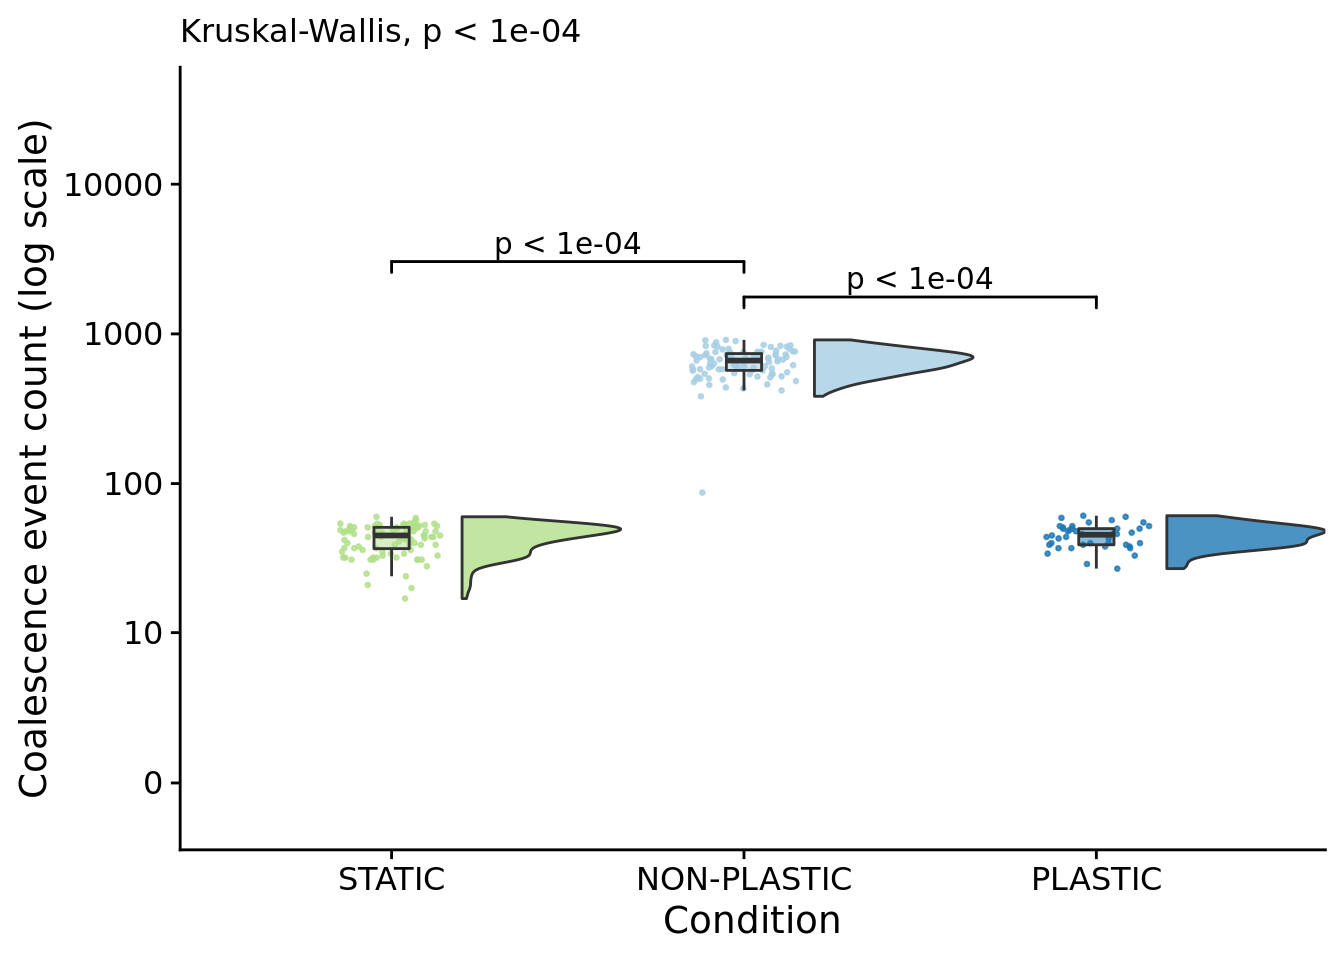
\includegraphics{supplemental-material_files/figure-latex/unnamed-chunk-16-1.pdf}

\begin{Shaded}
\begin{Highlighting}[]
\KeywordTok{kruskal.test}\NormalTok{(}
  \DataTypeTok{formula=}\NormalTok{phylo_mrca_changes}\OperatorTok{~}\NormalTok{condition,}
  \DataTypeTok{data=}\NormalTok{summary_data}
\NormalTok{)}
\end{Highlighting}
\end{Shaded}

\begin{verbatim}
## 
##  Kruskal-Wallis rank sum test
## 
## data:  phylo_mrca_changes by condition
## Kruskal-Wallis chi-squared = 175.46, df = 2, p-value < 2.2e-16
\end{verbatim}

\begin{Shaded}
\begin{Highlighting}[]
\KeywordTok{pairwise.wilcox.test}\NormalTok{(}
  \DataTypeTok{x=}\NormalTok{summary_data}\OperatorTok{$}\NormalTok{phylo_mrca_changes,}
  \DataTypeTok{g=}\NormalTok{summary_data}\OperatorTok{$}\NormalTok{condition,}
  \DataTypeTok{p.adjust.method=}\StringTok{"bonferroni"}\NormalTok{,}
\NormalTok{)}
\end{Highlighting}
\end{Shaded}

\begin{verbatim}
## 
##  Pairwise comparisons using Wilcoxon rank sum test with continuity correction 
## 
## data:  summary_data$phylo_mrca_changes and summary_data$condition 
## 
##         NON-PLASTIC PLASTIC
## PLASTIC <2e-16      -      
## STATIC  <2e-16      1      
## 
## P value adjustment method: bonferroni
\end{verbatim}

\begin{Shaded}
\begin{Highlighting}[]
\KeywordTok{paste}\NormalTok{(}
  \DataTypeTok{sep=}\StringTok{"; "}\NormalTok{,}
  \KeywordTok{paste0}\NormalTok{(}
    \StringTok{"PLASTIC median: "}\NormalTok{,}
    \KeywordTok{median}\NormalTok{(}\KeywordTok{filter}\NormalTok{(summary_data, condition}\OperatorTok{==}\StringTok{"PLASTIC"}\NormalTok{)}\OperatorTok{$}\NormalTok{phylo_mrca_changes)}
\NormalTok{  ),}
  \KeywordTok{paste0}\NormalTok{(}
    \StringTok{"STATIC median: "}\NormalTok{,}
    \KeywordTok{median}\NormalTok{(}\KeywordTok{filter}\NormalTok{(summary_data, condition}\OperatorTok{==}\StringTok{"STATIC"}\NormalTok{)}\OperatorTok{$}\NormalTok{phylo_mrca_changes)}
\NormalTok{  ),}
  \KeywordTok{paste0}\NormalTok{(}
    \StringTok{"NON-PLASTIC median: "}\NormalTok{,}
    \KeywordTok{median}\NormalTok{(}\KeywordTok{filter}\NormalTok{(summary_data, condition}\OperatorTok{==}\StringTok{"NON-PLASTIC"}\NormalTok{)}\OperatorTok{$}\NormalTok{phylo_mrca_changes)}
\NormalTok{  )}
\NormalTok{)}
\end{Highlighting}
\end{Shaded}

\begin{verbatim}
## [1] "PLASTIC median: 45.5; STATIC median: 45; NON-PLASTIC median: 663.5"
\end{verbatim}

\begin{Shaded}
\begin{Highlighting}[]
\KeywordTok{print}\NormalTok{(}\StringTok{"Wilcox rank sum test statistics:"}\NormalTok{)}
\end{Highlighting}
\end{Shaded}

\begin{verbatim}
## [1] "Wilcox rank sum test statistics:"
\end{verbatim}

\begin{Shaded}
\begin{Highlighting}[]
\ControlFlowTok{for}\NormalTok{ (pair }\ControlFlowTok{in}\NormalTok{ pairwise_comparisons) \{}
\NormalTok{  pair_data <-}\StringTok{ }\KeywordTok{filter}\NormalTok{(summary_data, condition }\OperatorTok\StringTok{ }\NormalTok{pair)}
\NormalTok{  pair_data}\OperatorTok{$}\NormalTok{condition <-}\StringTok{ }\KeywordTok{as.factor}\NormalTok{(pair_data}\OperatorTok{$}\NormalTok{condition)}
\NormalTok{  wt <-}\StringTok{ }\KeywordTok{wilcox.test}\NormalTok{(}
    \DataTypeTok{formula=}\NormalTok{phylo_mrca_changes}\OperatorTok{~}\NormalTok{condition,}
    \DataTypeTok{data=}\NormalTok{pair_data,}
    \DataTypeTok{exact=}\OtherTok{FALSE}\NormalTok{,}
    \DataTypeTok{paired=}\OtherTok{FALSE}
\NormalTok{  )}
  \KeywordTok{print}\NormalTok{(}\KeywordTok{paste0}\NormalTok{(pair[}\DecValTok{1}\NormalTok{], }\StringTok{"<-->"}\NormalTok{, pair[}\DecValTok{2}\NormalTok{], }\StringTok{": W="}\NormalTok{,wt}\OperatorTok{$}\NormalTok{statistic))}
\NormalTok{\}}
\end{Highlighting}
\end{Shaded}

\begin{verbatim}
## [1] "STATIC<-->NON-PLASTIC: W=10000"
## [1] "STATIC<-->PLASTIC: W=2215"
## [1] "PLASTIC<-->NON-PLASTIC: W=4200"
\end{verbatim}

\hypertarget{average-number-of-generations-between-coalescence-events}{%
\subsection{Average number of generations between coalescence events}\label{average-number-of-generations-between-coalescence-events}}

\begin{Shaded}
\begin{Highlighting}[]
\CommentTok{# Compute frequency of coalescence events}
\NormalTok{summary_data}\OperatorTok{$}\NormalTok{generations_per_mrca_change <-}\StringTok{ }\NormalTok{summary_data}\OperatorTok{$}\NormalTok{time_average_generation }\OperatorTok{/}\StringTok{ }\NormalTok{summary_data}\OperatorTok{$}\NormalTok{phylo_mrca_changes}

\CommentTok{# Compute manual labels for geom_signif}
\NormalTok{stat.test <-}\StringTok{ }\NormalTok{summary_data }\OperatorTok
\StringTok{  }\KeywordTok{wilcox_test}\NormalTok{(generations_per_mrca_change }\OperatorTok{~}\StringTok{ }\NormalTok{condition) }\OperatorTok
\StringTok{  }\KeywordTok{adjust_pvalue}\NormalTok{(}\DataTypeTok{method =} \StringTok{"bonferroni"}\NormalTok{) }\OperatorTok
\StringTok{  }\KeywordTok{add_significance}\NormalTok{() }\OperatorTok
\StringTok{  }\KeywordTok{add_xy_position}\NormalTok{(}\DataTypeTok{x=}\StringTok{"condition"}\NormalTok{)}
\CommentTok{# Tweak y.position manually to account for scaled axis (edge case that triggers bad behavior in geom_signif)}
\NormalTok{stat.test}\OperatorTok{$}\NormalTok{manual_position <-}\StringTok{  }\NormalTok{stat.test}\OperatorTok{$}\NormalTok{y.position}
\NormalTok{stat.test}\OperatorTok{$}\NormalTok{label <-}\StringTok{ }\KeywordTok{mapply}\NormalTok{(p_label,stat.test}\OperatorTok{$}\NormalTok{p.adj)}

\NormalTok{summary_data}\OperatorTok{$}\NormalTok{is_outlier <-}\StringTok{ }\KeywordTok{mapply}\NormalTok{(}
\NormalTok{  is_outlier,}
\NormalTok{  summary_data}\OperatorTok{$}\NormalTok{generations_per_mrca_change,}
\NormalTok{  summary_data}\OperatorTok{$}\NormalTok{condition,}
  \DataTypeTok{MoreArgs=}\KeywordTok{list}\NormalTok{(}\DataTypeTok{data=}\NormalTok{summary_data, }\DataTypeTok{column=}\StringTok{"generations_per_mrca_change"}\NormalTok{)}
\NormalTok{)}

\NormalTok{coalescence_events_freq_fig <-}\StringTok{ }\KeywordTok{ggplot}\NormalTok{(}
\NormalTok{    summary_data,}
    \KeywordTok{aes}\NormalTok{(}\DataTypeTok{x=}\NormalTok{condition, }\DataTypeTok{y=}\NormalTok{generations_per_mrca_change, }\DataTypeTok{fill=}\NormalTok{condition)}
\NormalTok{  ) }\OperatorTok{+}
\StringTok{  }\KeywordTok{geom_flat_violin}\NormalTok{(}
    \CommentTok{# data=filter(summary_data,is_outlier==FALSE),}
    \DataTypeTok{scale=}\StringTok{"width"}\NormalTok{,}
    \DataTypeTok{position =} \KeywordTok{position_nudge}\NormalTok{(}\DataTypeTok{x =} \FloatTok{.2}\NormalTok{, }\DataTypeTok{y =} \DecValTok{0}\NormalTok{),}
    \DataTypeTok{alpha =} \FloatTok{.8}
\NormalTok{  ) }\OperatorTok{+}
\StringTok{  }\KeywordTok{geom_point}\NormalTok{(}
    \DataTypeTok{mapping=}\KeywordTok{aes}\NormalTok{(}\DataTypeTok{color=}\NormalTok{condition),}
    \DataTypeTok{position =} \KeywordTok{position_jitter}\NormalTok{(}\DataTypeTok{width =} \FloatTok{.15}\NormalTok{),}
    \DataTypeTok{size =} \FloatTok{.5}\NormalTok{,}
    \DataTypeTok{alpha =} \FloatTok{0.8}
\NormalTok{  ) }\OperatorTok{+}
\StringTok{  }\KeywordTok{geom_boxplot}\NormalTok{(}
    \DataTypeTok{width =} \FloatTok{.1}\NormalTok{,}
    \DataTypeTok{outlier.shape =} \OtherTok{NA}\NormalTok{,}
    \DataTypeTok{alpha =} \FloatTok{0.5}
\NormalTok{  ) }\OperatorTok{+}
\StringTok{  }\KeywordTok{scale_x_discrete}\NormalTok{(}
    \DataTypeTok{name=}\StringTok{"Condition"}\NormalTok{,}
    \DataTypeTok{limits=}\NormalTok{condition_order,}
    \DataTypeTok{labels=}\NormalTok{condition_order}
\NormalTok{  ) }\OperatorTok{+}
\StringTok{  }\KeywordTok{scale_y_continuous}\NormalTok{(}
    \DataTypeTok{name=}\StringTok{"Avg. generations between coalescence events"}\NormalTok{,}
    \DataTypeTok{limits=}\KeywordTok{c}\NormalTok{(}\DecValTok{0}\NormalTok{, }\DecValTok{2000}\NormalTok{),}
    \DataTypeTok{breaks=}\KeywordTok{seq}\NormalTok{(}\DecValTok{0}\NormalTok{, }\DecValTok{2000}\NormalTok{, }\DecValTok{500}\NormalTok{)}
\NormalTok{  ) }\OperatorTok{+}
\StringTok{  }\KeywordTok{scale_fill_brewer}\NormalTok{(}
    \DataTypeTok{palette=}\NormalTok{cb_palette}
\NormalTok{  ) }\OperatorTok{+}
\StringTok{  }\KeywordTok{scale_color_brewer}\NormalTok{(}
    \DataTypeTok{palette=}\NormalTok{cb_palette}
\NormalTok{  ) }\OperatorTok{+}
\StringTok{  }\CommentTok{# coord_flip() +}
\StringTok{  }\KeywordTok{labs}\NormalTok{(}
    \DataTypeTok{subtitle=}\KeywordTok{paste0}\NormalTok{(}
      \StringTok{"Kruskal-Wallis, "}\NormalTok{,}
      \KeywordTok{p_label}\NormalTok{(}\KeywordTok{signif}\NormalTok{(}\KeywordTok{kruskal.test}\NormalTok{(}\DataTypeTok{formula=}\NormalTok{generations_per_mrca_change}\OperatorTok{~}\NormalTok{condition, }\DataTypeTok{data=}\NormalTok{summary_data)}\OperatorTok{$}\NormalTok{p.value,}\DataTypeTok{digits=}\DecValTok{4}\NormalTok{))}
\NormalTok{    )}
\NormalTok{  ) }\OperatorTok{+}
\StringTok{  }\NormalTok{ggsignif}\OperatorTok{::}\KeywordTok{geom_signif}\NormalTok{(}
    \DataTypeTok{data=}\KeywordTok{filter}\NormalTok{(stat.test, p.adj }\OperatorTok{<=}\StringTok{ }\NormalTok{alpha),}
    \KeywordTok{aes}\NormalTok{(}\DataTypeTok{xmin=}\NormalTok{group1,}\DataTypeTok{xmax=}\NormalTok{group2,}\DataTypeTok{annotations=}\NormalTok{label,}\DataTypeTok{y_position=}\NormalTok{manual_position),}
    \DataTypeTok{manual=}\OtherTok{TRUE}\NormalTok{,}
    \DataTypeTok{inherit.aes=}\OtherTok{FALSE}
\NormalTok{  ) }\OperatorTok{+}
\StringTok{  }\KeywordTok{theme}\NormalTok{(}
    \DataTypeTok{legend.position=}\StringTok{"none"}
\NormalTok{  )}
\end{Highlighting}
\end{Shaded}

\begin{verbatim}
## Warning: Ignoring unknown aesthetics: xmin, xmax, annotations, y_position
\end{verbatim}

\begin{Shaded}
\begin{Highlighting}[]
\KeywordTok{ggsave}\NormalTok{(}
  \KeywordTok{paste0}\NormalTok{(working_directory, }\StringTok{"plots/"}\NormalTok{, }\StringTok{"generations-between-selective-sweeps.png"}\NormalTok{),}
  \DataTypeTok{width=}\DecValTok{5}\NormalTok{,}
  \DataTypeTok{height=}\DecValTok{5}
\NormalTok{)}
\NormalTok{coalescence_events_freq_fig}
\end{Highlighting}
\end{Shaded}

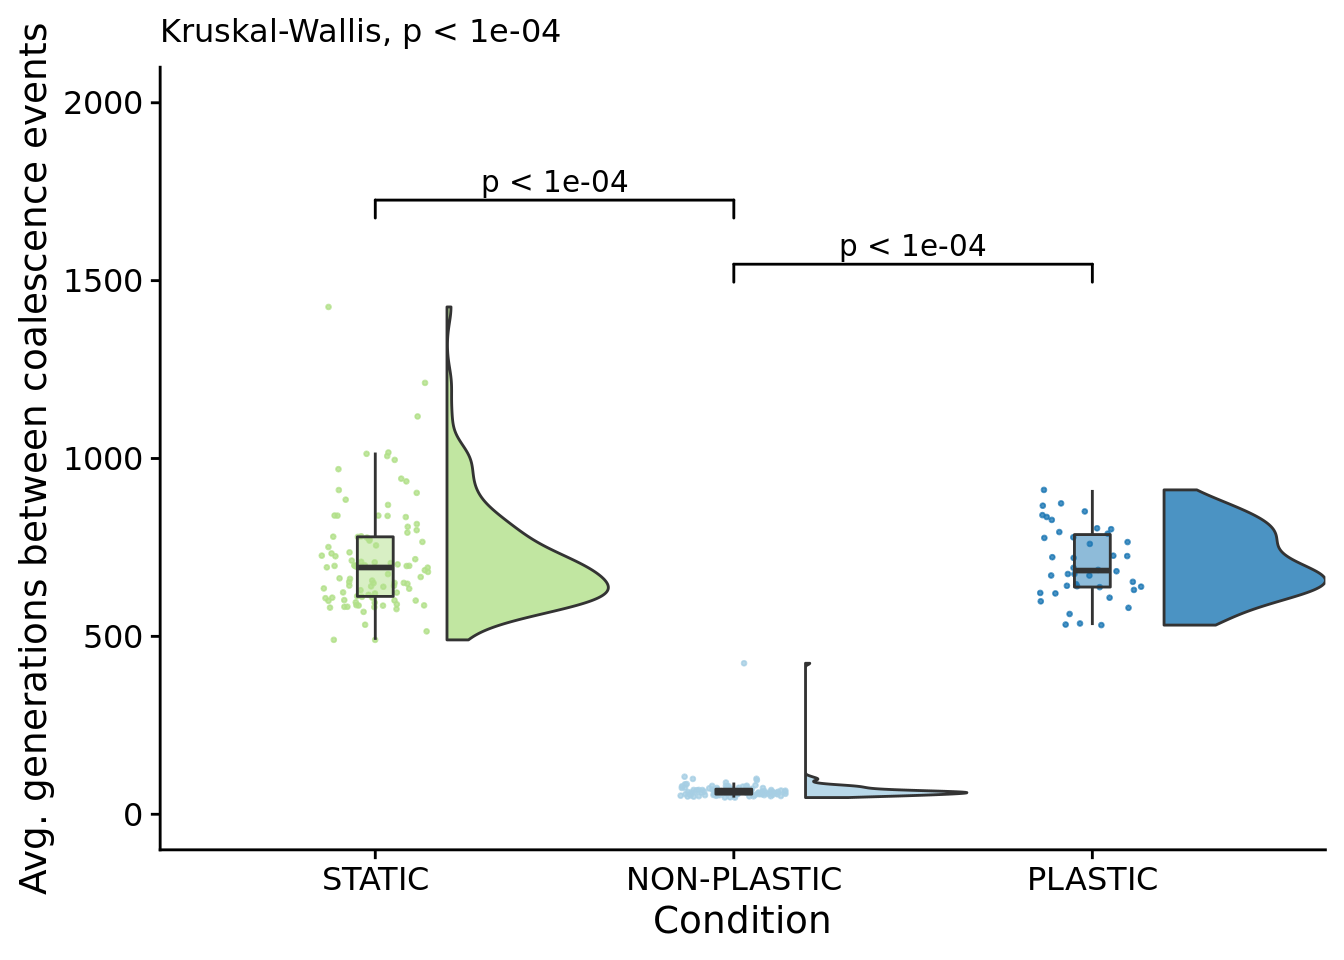
\includegraphics{supplemental-material_files/figure-latex/unnamed-chunk-18-1.pdf}

\begin{Shaded}
\begin{Highlighting}[]
\KeywordTok{kruskal.test}\NormalTok{(}
  \DataTypeTok{formula=}\NormalTok{generations_per_mrca_change}\OperatorTok{~}\NormalTok{condition,}
  \DataTypeTok{data=}\NormalTok{summary_data}
\NormalTok{)}
\end{Highlighting}
\end{Shaded}

\begin{verbatim}
## 
##  Kruskal-Wallis rank sum test
## 
## data:  generations_per_mrca_change by condition
## Kruskal-Wallis chi-squared = 175.33, df = 2, p-value < 2.2e-16
\end{verbatim}

\begin{Shaded}
\begin{Highlighting}[]
\KeywordTok{pairwise.wilcox.test}\NormalTok{(}
  \DataTypeTok{x=}\NormalTok{summary_data}\OperatorTok{$}\NormalTok{generations_per_mrca_change,}
  \DataTypeTok{g=}\NormalTok{summary_data}\OperatorTok{$}\NormalTok{condition,}
  \DataTypeTok{p.adjust.method=}\StringTok{"bonferroni"}\NormalTok{,}
\NormalTok{)}
\end{Highlighting}
\end{Shaded}

\begin{verbatim}
## 
##  Pairwise comparisons using Wilcoxon rank sum test with continuity correction 
## 
## data:  summary_data$generations_per_mrca_change and summary_data$condition 
## 
##         NON-PLASTIC PLASTIC
## PLASTIC <2e-16      -      
## STATIC  <2e-16      1      
## 
## P value adjustment method: bonferroni
\end{verbatim}

\begin{Shaded}
\begin{Highlighting}[]
\KeywordTok{paste}\NormalTok{(}
  \DataTypeTok{sep=}\StringTok{"; "}\NormalTok{,}
  \KeywordTok{paste0}\NormalTok{(}
    \StringTok{"PLASTIC median: "}\NormalTok{,}
    \KeywordTok{median}\NormalTok{(}\KeywordTok{filter}\NormalTok{(summary_data, condition}\OperatorTok{==}\StringTok{"PLASTIC"}\NormalTok{)}\OperatorTok{$}\NormalTok{generations_per_mrca_change)}
\NormalTok{  ),}
  \KeywordTok{paste0}\NormalTok{(}
    \StringTok{"STATIC median: "}\NormalTok{,}
    \KeywordTok{median}\NormalTok{(}\KeywordTok{filter}\NormalTok{(summary_data, condition}\OperatorTok{==}\StringTok{"STATIC"}\NormalTok{)}\OperatorTok{$}\NormalTok{generations_per_mrca_change)}
\NormalTok{  ),}
  \KeywordTok{paste0}\NormalTok{(}
    \StringTok{"NON-PLASTIC median: "}\NormalTok{,}
    \KeywordTok{median}\NormalTok{(}\KeywordTok{filter}\NormalTok{(summary_data, condition}\OperatorTok{==}\StringTok{"NON-PLASTIC"}\NormalTok{)}\OperatorTok{$}\NormalTok{generations_per_mrca_change)}
\NormalTok{  )}
\NormalTok{)}
\end{Highlighting}
\end{Shaded}

\begin{verbatim}
## [1] "PLASTIC median: 685.001780758557; STATIC median: 693.676265008576; NON-PLASTIC median: 62.0184902295191"
\end{verbatim}

\begin{Shaded}
\begin{Highlighting}[]
\KeywordTok{print}\NormalTok{(}\StringTok{"Wilcox rank sum test statistics:"}\NormalTok{)}
\end{Highlighting}
\end{Shaded}

\begin{verbatim}
## [1] "Wilcox rank sum test statistics:"
\end{verbatim}

\begin{Shaded}
\begin{Highlighting}[]
\ControlFlowTok{for}\NormalTok{ (pair }\ControlFlowTok{in}\NormalTok{ pairwise_comparisons) \{}
\NormalTok{  pair_data <-}\StringTok{ }\KeywordTok{filter}\NormalTok{(summary_data, condition }\OperatorTok\StringTok{ }\NormalTok{pair)}
\NormalTok{  pair_data}\OperatorTok{$}\NormalTok{condition <-}\StringTok{ }\KeywordTok{as.factor}\NormalTok{(pair_data}\OperatorTok{$}\NormalTok{condition)}
\NormalTok{  wt <-}\StringTok{ }\KeywordTok{wilcox.test}\NormalTok{(}
    \DataTypeTok{formula=}\NormalTok{generations_per_mrca_change}\OperatorTok{~}\NormalTok{condition,}
    \DataTypeTok{data=}\NormalTok{pair_data,}
    \DataTypeTok{exact=}\OtherTok{FALSE}\NormalTok{,}
    \DataTypeTok{paired=}\OtherTok{FALSE}
\NormalTok{  )}
  \KeywordTok{print}\NormalTok{(}\KeywordTok{paste0}\NormalTok{(pair[}\DecValTok{1}\NormalTok{], }\StringTok{"<-->"}\NormalTok{, pair[}\DecValTok{2}\NormalTok{], }\StringTok{": W="}\NormalTok{,wt}\OperatorTok{$}\NormalTok{statistic))}
\NormalTok{\}}
\end{Highlighting}
\end{Shaded}

\begin{verbatim}
## [1] "STATIC<-->NON-PLASTIC: W=0"
## [1] "STATIC<-->PLASTIC: W=2151"
## [1] "PLASTIC<-->NON-PLASTIC: W=0"
\end{verbatim}

\hypertarget{phenotypic-volatility-along-the-dominant-lineage}{%
\section{Phenotypic volatility along the dominant lineage}\label{phenotypic-volatility-along-the-dominant-lineage}}

\begin{Shaded}
\begin{Highlighting}[]
\CommentTok{# Compute manual labels for geom_signif}
\NormalTok{stat.test <-}\StringTok{ }\NormalTok{summary_data }\OperatorTok
\StringTok{  }\KeywordTok{wilcox_test}\NormalTok{(dominant_lineage_trait_volatility }\OperatorTok{~}\StringTok{ }\NormalTok{condition) }\OperatorTok
\StringTok{  }\KeywordTok{adjust_pvalue}\NormalTok{(}\DataTypeTok{method =} \StringTok{"bonferroni"}\NormalTok{) }\OperatorTok
\StringTok{  }\KeywordTok{add_significance}\NormalTok{() }\OperatorTok
\StringTok{  }\KeywordTok{add_xy_position}\NormalTok{(}\DataTypeTok{x=}\StringTok{"condition"}\NormalTok{, }\DataTypeTok{step.increase=}\DecValTok{1}\NormalTok{)}
\CommentTok{# Tweak y.position manually to account for scaled axis (edge case that triggers bad behavior in geom_signif)}
\NormalTok{stat.test}\OperatorTok{$}\NormalTok{manual_position <-}\StringTok{  }\KeywordTok{log10}\NormalTok{(stat.test}\OperatorTok{$}\NormalTok{y.position) }\OperatorTok{*}\StringTok{ }\KeywordTok{c}\NormalTok{(}\FloatTok{1.0}\NormalTok{,}\FloatTok{1.0}\NormalTok{,}\FloatTok{1.03}\NormalTok{)}
\NormalTok{stat.test}\OperatorTok{$}\NormalTok{label <-}\StringTok{ }\KeywordTok{mapply}\NormalTok{(p_label,stat.test}\OperatorTok{$}\NormalTok{p.adj)}

\NormalTok{summary_data}\OperatorTok{$}\NormalTok{is_outlier <-}\StringTok{ }\KeywordTok{mapply}\NormalTok{(}
\NormalTok{  is_outlier,}
\NormalTok{  summary_data}\OperatorTok{$}\NormalTok{dominant_lineage_trait_volatility,}
\NormalTok{  summary_data}\OperatorTok{$}\NormalTok{condition,}
  \DataTypeTok{MoreArgs=}\KeywordTok{list}\NormalTok{(}\DataTypeTok{data=}\NormalTok{summary_data, }\DataTypeTok{column=}\StringTok{"dominant_lineage_trait_volatility"}\NormalTok{)}
\NormalTok{)}

\NormalTok{phenotypic_volatility_fig <-}\StringTok{ }\KeywordTok{ggplot}\NormalTok{(}
\NormalTok{    summary_data,}
    \KeywordTok{aes}\NormalTok{(}\DataTypeTok{x=}\NormalTok{condition, }\DataTypeTok{y=}\NormalTok{dominant_lineage_trait_volatility, }\DataTypeTok{fill=}\NormalTok{condition)}
\NormalTok{  ) }\OperatorTok{+}
\StringTok{  }\KeywordTok{geom_flat_violin}\NormalTok{(}
    \CommentTok{# data=filter(summary_data,is_outlier==FALSE),}
    \DataTypeTok{scale=}\StringTok{"width"}\NormalTok{,}
    \DataTypeTok{position =} \KeywordTok{position_nudge}\NormalTok{(}\DataTypeTok{x =} \FloatTok{.2}\NormalTok{, }\DataTypeTok{y =} \DecValTok{0}\NormalTok{),}
    \DataTypeTok{alpha =} \FloatTok{.8}
\NormalTok{  ) }\OperatorTok{+}
\StringTok{  }\KeywordTok{geom_point}\NormalTok{(}
    \DataTypeTok{mapping=}\KeywordTok{aes}\NormalTok{(}\DataTypeTok{color=}\NormalTok{condition),}
    \DataTypeTok{position =} \KeywordTok{position_jitter}\NormalTok{(}\DataTypeTok{width =} \FloatTok{.15}\NormalTok{),}
    \DataTypeTok{size =} \FloatTok{.5}\NormalTok{,}
    \DataTypeTok{alpha =} \FloatTok{0.8}
\NormalTok{  ) }\OperatorTok{+}
\StringTok{  }\KeywordTok{geom_boxplot}\NormalTok{(}
    \DataTypeTok{width =} \FloatTok{.1}\NormalTok{,}
    \DataTypeTok{outlier.shape =} \OtherTok{NA}\NormalTok{,}
    \DataTypeTok{alpha =} \FloatTok{0.5}
\NormalTok{  ) }\OperatorTok{+}
\StringTok{  }\KeywordTok{scale_x_discrete}\NormalTok{(}
    \DataTypeTok{name=}\StringTok{"Condition"}\NormalTok{,}
    \DataTypeTok{limits=}\NormalTok{condition_order,}
    \DataTypeTok{labels=}\NormalTok{condition_order}
\NormalTok{  ) }\OperatorTok{+}
\StringTok{  }\KeywordTok{scale_y_continuous}\NormalTok{(}
    \DataTypeTok{name=}\StringTok{"Phenotypic volatility (log scale)"}\NormalTok{,}
    \DataTypeTok{trans=}\KeywordTok{pseudo_log_trans}\NormalTok{(}\DataTypeTok{sigma =} \DecValTok{1}\NormalTok{, }\DataTypeTok{base =} \DecValTok{10}\NormalTok{),}
    \DataTypeTok{breaks=}\KeywordTok{c}\NormalTok{(}\DecValTok{0}\NormalTok{, }\DecValTok{10}\NormalTok{, }\DecValTok{100}\NormalTok{, }\DecValTok{1000}\NormalTok{, }\DecValTok{10000}\NormalTok{),}
    \DataTypeTok{limits=}\KeywordTok{c}\NormalTok{(}\OperatorTok{-}\DecValTok{1}\NormalTok{, }\DecValTok{35000}\NormalTok{)}
\NormalTok{  ) }\OperatorTok{+}
\StringTok{  }\KeywordTok{scale_fill_brewer}\NormalTok{(}
    \DataTypeTok{palette=}\NormalTok{cb_palette}
\NormalTok{  ) }\OperatorTok{+}
\StringTok{  }\KeywordTok{scale_color_brewer}\NormalTok{(}
    \DataTypeTok{palette=}\NormalTok{cb_palette}
\NormalTok{  ) }\OperatorTok{+}
\StringTok{  }\KeywordTok{labs}\NormalTok{(}
    \DataTypeTok{subtitle=}\KeywordTok{paste0}\NormalTok{(}
      \StringTok{"Kruskal-Wallis, "}\NormalTok{,}
      \KeywordTok{p_label}\NormalTok{(}\KeywordTok{signif}\NormalTok{(}\KeywordTok{kruskal.test}\NormalTok{(}\DataTypeTok{formula=}\NormalTok{dominant_lineage_trait_volatility}\OperatorTok{~}\NormalTok{condition, }\DataTypeTok{data=}\NormalTok{summary_data)}\OperatorTok{$}\NormalTok{p.value,}\DataTypeTok{digits=}\DecValTok{4}\NormalTok{))}
\NormalTok{    )}
\NormalTok{  ) }\OperatorTok{+}
\StringTok{  }\NormalTok{ggsignif}\OperatorTok{::}\KeywordTok{geom_signif}\NormalTok{(}
    \DataTypeTok{data=}\KeywordTok{filter}\NormalTok{(stat.test, p.adj}\OperatorTok{<=}\NormalTok{alpha),}
    \KeywordTok{aes}\NormalTok{(}\DataTypeTok{xmin=}\NormalTok{group1,}\DataTypeTok{xmax=}\NormalTok{group2,}\DataTypeTok{annotations=}\NormalTok{label,}\DataTypeTok{y_position=}\NormalTok{manual_position),}
    \DataTypeTok{manual=}\OtherTok{TRUE}\NormalTok{,}
    \DataTypeTok{inherit.aes=}\OtherTok{FALSE}
\NormalTok{  ) }\OperatorTok{+}
\StringTok{  }\CommentTok{# coord_flip() +}
\StringTok{  }\KeywordTok{theme}\NormalTok{(}
    \DataTypeTok{legend.position=}\StringTok{"none"}
\NormalTok{  )}
\end{Highlighting}
\end{Shaded}

\begin{verbatim}
## Warning: Ignoring unknown aesthetics: xmin, xmax, annotations, y_position
\end{verbatim}

\begin{Shaded}
\begin{Highlighting}[]
\KeywordTok{ggsave}\NormalTok{(}
  \KeywordTok{paste0}\NormalTok{(working_directory, }\StringTok{"plots/"}\NormalTok{, }\StringTok{"phenotypic-volatility.pdf"}\NormalTok{),}
  \DataTypeTok{width=}\DecValTok{5}\NormalTok{,}
  \DataTypeTok{height=}\DecValTok{5}
\NormalTok{)}
\NormalTok{phenotypic_volatility_fig}
\end{Highlighting}
\end{Shaded}

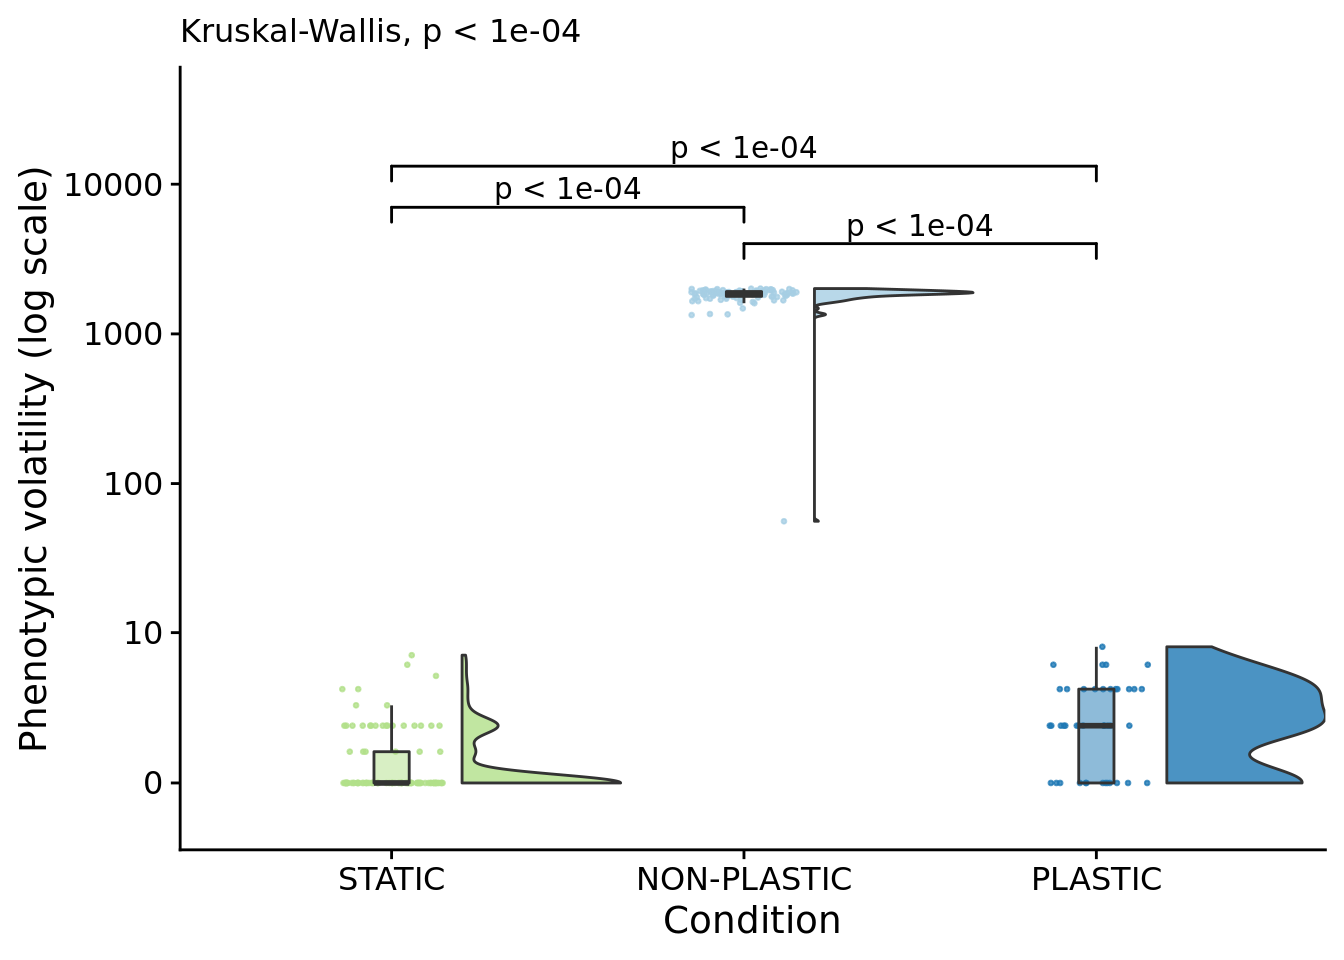
\includegraphics{supplemental-material_files/figure-latex/unnamed-chunk-20-1.pdf}

\begin{Shaded}
\begin{Highlighting}[]
\KeywordTok{kruskal.test}\NormalTok{(}
  \DataTypeTok{formula=}\NormalTok{dominant_lineage_trait_volatility}\OperatorTok{~}\NormalTok{condition,}
  \DataTypeTok{data=}\NormalTok{summary_data}
\NormalTok{)}
\end{Highlighting}
\end{Shaded}

\begin{verbatim}
## 
##  Kruskal-Wallis rank sum test
## 
## data:  dominant_lineage_trait_volatility by condition
## Kruskal-Wallis chi-squared = 190.78, df = 2, p-value < 2.2e-16
\end{verbatim}

\begin{Shaded}
\begin{Highlighting}[]
\KeywordTok{pairwise.wilcox.test}\NormalTok{(}
  \DataTypeTok{x=}\NormalTok{summary_data}\OperatorTok{$}\NormalTok{dominant_lineage_trait_volatility,}
  \DataTypeTok{g=}\NormalTok{summary_data}\OperatorTok{$}\NormalTok{condition,}
  \DataTypeTok{p.adjust.method=}\StringTok{"bonferroni"}\NormalTok{,}
\NormalTok{)}
\end{Highlighting}
\end{Shaded}

\begin{verbatim}
## 
##  Pairwise comparisons using Wilcoxon rank sum test with continuity correction 
## 
## data:  summary_data$dominant_lineage_trait_volatility and summary_data$condition 
## 
##         NON-PLASTIC PLASTIC
## PLASTIC < 2e-16     -      
## STATIC  < 2e-16     8.7e-07
## 
## P value adjustment method: bonferroni
\end{verbatim}

\begin{Shaded}
\begin{Highlighting}[]
\KeywordTok{paste}\NormalTok{(}
  \DataTypeTok{sep=}\StringTok{"; "}\NormalTok{,}
  \KeywordTok{paste0}\NormalTok{(}
    \StringTok{"PLASTIC median: "}\NormalTok{,}
    \KeywordTok{median}\NormalTok{(}\KeywordTok{filter}\NormalTok{(summary_data, condition}\OperatorTok{==}\StringTok{"PLASTIC"}\NormalTok{)}\OperatorTok{$}\NormalTok{dominant_lineage_trait_volatility)}
\NormalTok{  ),}
  \KeywordTok{paste0}\NormalTok{(}
    \StringTok{"STATIC median: "}\NormalTok{,}
    \KeywordTok{median}\NormalTok{(}\KeywordTok{filter}\NormalTok{(summary_data, condition}\OperatorTok{==}\StringTok{"STATIC"}\NormalTok{)}\OperatorTok{$}\NormalTok{dominant_lineage_trait_volatility)}
\NormalTok{  ),}
  \KeywordTok{paste0}\NormalTok{(}
    \StringTok{"NON-PLASTIC median: "}\NormalTok{,}
    \KeywordTok{median}\NormalTok{(}\KeywordTok{filter}\NormalTok{(summary_data, condition}\OperatorTok{==}\StringTok{"NON-PLASTIC"}\NormalTok{)}\OperatorTok{$}\NormalTok{dominant_lineage_trait_volatility)}
\NormalTok{  )}
\NormalTok{)}
\end{Highlighting}
\end{Shaded}

\begin{verbatim}
## [1] "PLASTIC median: 2; STATIC median: 0; NON-PLASTIC median: 1868"
\end{verbatim}

\begin{Shaded}
\begin{Highlighting}[]
\KeywordTok{print}\NormalTok{(}\StringTok{"Wilcox rank sum test statistics:"}\NormalTok{)}
\end{Highlighting}
\end{Shaded}

\begin{verbatim}
## [1] "Wilcox rank sum test statistics:"
\end{verbatim}

\begin{Shaded}
\begin{Highlighting}[]
\ControlFlowTok{for}\NormalTok{ (pair }\ControlFlowTok{in}\NormalTok{ pairwise_comparisons) \{}
\NormalTok{  pair_data <-}\StringTok{ }\KeywordTok{filter}\NormalTok{(summary_data, condition }\OperatorTok\StringTok{ }\NormalTok{pair)}
\NormalTok{  pair_data}\OperatorTok{$}\NormalTok{condition <-}\StringTok{ }\KeywordTok{as.factor}\NormalTok{(pair_data}\OperatorTok{$}\NormalTok{condition)}
\NormalTok{  wt <-}\StringTok{ }\KeywordTok{wilcox.test}\NormalTok{(}
    \DataTypeTok{formula=}\NormalTok{dominant_lineage_trait_volatility}\OperatorTok{~}\NormalTok{condition,}
    \DataTypeTok{data=}\NormalTok{pair_data,}
    \DataTypeTok{exact=}\OtherTok{FALSE}\NormalTok{,}
    \DataTypeTok{paired=}\OtherTok{FALSE}
\NormalTok{  )}
  \KeywordTok{print}\NormalTok{(}\KeywordTok{paste0}\NormalTok{(pair[}\DecValTok{1}\NormalTok{], }\StringTok{"<-->"}\NormalTok{, pair[}\DecValTok{2}\NormalTok{], }\StringTok{": W="}\NormalTok{,wt}\OperatorTok{$}\NormalTok{statistic))}
\NormalTok{\}}
\end{Highlighting}
\end{Shaded}

\begin{verbatim}
## [1] "STATIC<-->NON-PLASTIC: W=10000"
## [1] "STATIC<-->PLASTIC: W=3116.5"
## [1] "PLASTIC<-->NON-PLASTIC: W=4200"
\end{verbatim}

\hypertarget{phenotypic-volatility-normalized-by-generations-elapsed}{%
\subsection{Phenotypic volatility normalized by generations elapsed}\label{phenotypic-volatility-normalized-by-generations-elapsed}}

\begin{Shaded}
\begin{Highlighting}[]
\NormalTok{summary_data}\OperatorTok{$}\NormalTok{dominant_lineage_trait_volatility_per_generation <-}\StringTok{ }\NormalTok{summary_data}\OperatorTok{$}\NormalTok{dominant_lineage_trait_volatility }\OperatorTok{/}\StringTok{ }\NormalTok{summary_data}\OperatorTok{$}\NormalTok{dominant_generation_born}

\KeywordTok{ggplot}\NormalTok{(summary_data, }\KeywordTok{aes}\NormalTok{(}\DataTypeTok{x=}\NormalTok{condition, }\DataTypeTok{y=}\NormalTok{dominant_lineage_trait_volatility_per_generation, }\DataTypeTok{fill=}\NormalTok{condition)) }\OperatorTok{+}
\StringTok{  }\KeywordTok{geom_flat_violin}\NormalTok{(}
    \DataTypeTok{position =} \KeywordTok{position_nudge}\NormalTok{(}\DataTypeTok{x =} \FloatTok{.2}\NormalTok{, }\DataTypeTok{y =} \DecValTok{0}\NormalTok{),}
    \DataTypeTok{alpha =} \FloatTok{.8}
\NormalTok{  ) }\OperatorTok{+}
\StringTok{  }\KeywordTok{geom_point}\NormalTok{(}
    \DataTypeTok{mapping=}\KeywordTok{aes}\NormalTok{(}\DataTypeTok{color=}\NormalTok{condition),}
    \DataTypeTok{position =} \KeywordTok{position_jitter}\NormalTok{(}\DataTypeTok{width =} \FloatTok{.15}\NormalTok{),}
    \DataTypeTok{size =} \FloatTok{.5}\NormalTok{,}
    \DataTypeTok{alpha =} \FloatTok{0.8}
\NormalTok{  ) }\OperatorTok{+}
\StringTok{  }\KeywordTok{geom_boxplot}\NormalTok{(}
    \DataTypeTok{width =} \FloatTok{.1}\NormalTok{,}
    \DataTypeTok{outlier.shape =} \OtherTok{NA}\NormalTok{,}
    \DataTypeTok{alpha =} \FloatTok{0.5}
\NormalTok{  ) }\OperatorTok{+}
\StringTok{  }\KeywordTok{scale_x_discrete}\NormalTok{(}
    \DataTypeTok{name=}\StringTok{"Condition"}\NormalTok{,}
    \DataTypeTok{limits=}\NormalTok{condition_order}
\NormalTok{  ) }\OperatorTok{+}
\StringTok{  }\KeywordTok{scale_fill_brewer}\NormalTok{(}
    \DataTypeTok{palette=}\NormalTok{cb_palette}
\NormalTok{  ) }\OperatorTok{+}
\StringTok{  }\KeywordTok{scale_color_brewer}\NormalTok{(}
    \DataTypeTok{palette=}\NormalTok{cb_palette}
\NormalTok{  ) }\OperatorTok{+}
\StringTok{  }\KeywordTok{theme}\NormalTok{(}
    \DataTypeTok{legend.position=}\StringTok{"none"}
\NormalTok{  )}
\end{Highlighting}
\end{Shaded}

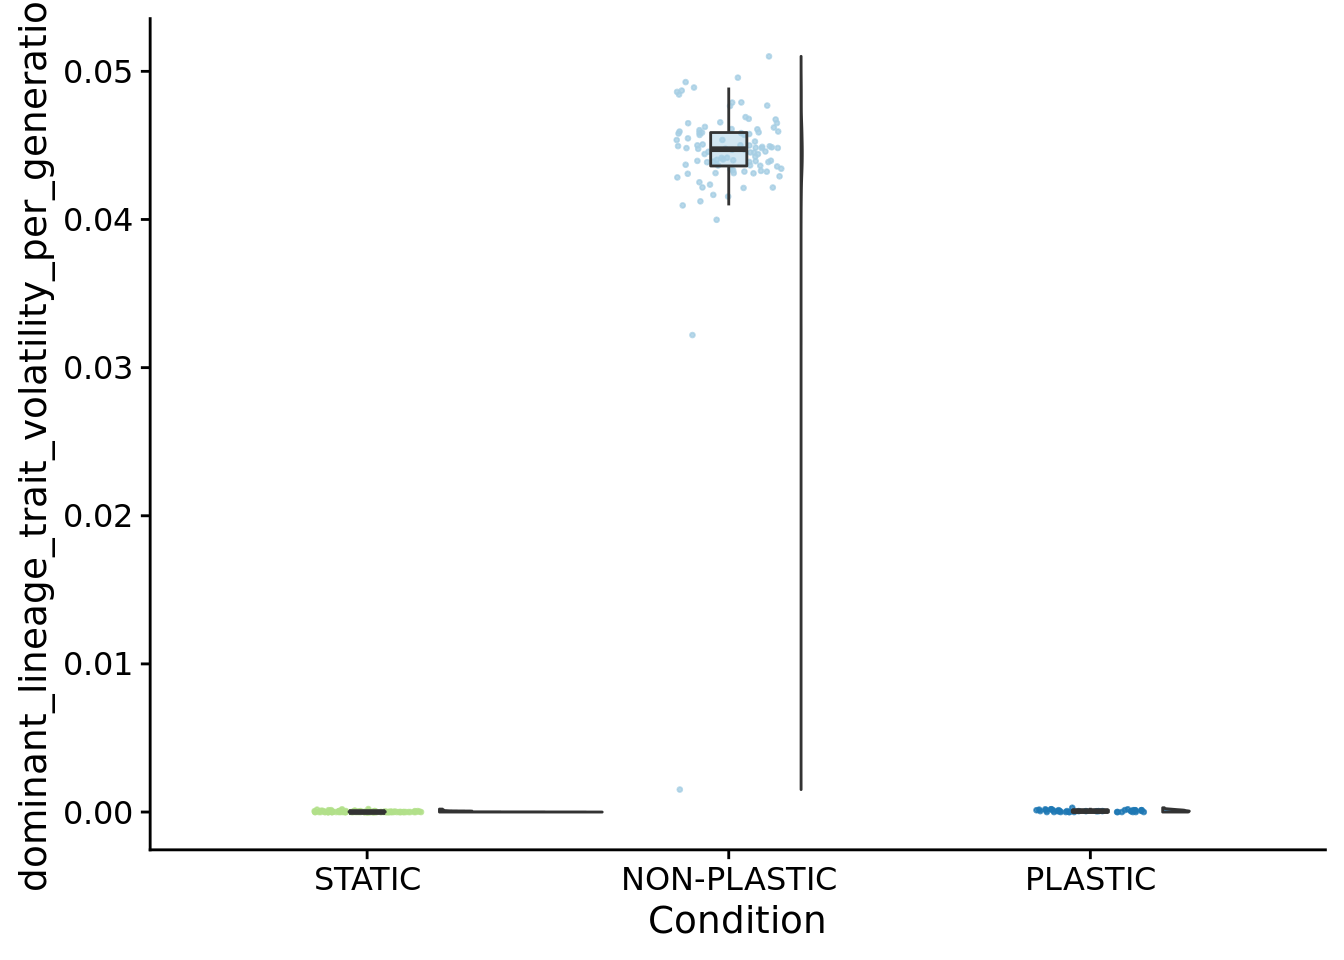
\includegraphics{supplemental-material_files/figure-latex/unnamed-chunk-22-1.pdf}

\begin{Shaded}
\begin{Highlighting}[]
\KeywordTok{kruskal.test}\NormalTok{(}
  \DataTypeTok{formula=}\NormalTok{dominant_lineage_trait_volatility_per_generation}\OperatorTok{~}\NormalTok{condition,}
  \DataTypeTok{data=}\NormalTok{summary_data}
\NormalTok{)}
\end{Highlighting}
\end{Shaded}

\begin{verbatim}
## 
##  Kruskal-Wallis rank sum test
## 
## data:  dominant_lineage_trait_volatility_per_generation by condition
## Kruskal-Wallis chi-squared = 189.62, df = 2, p-value < 2.2e-16
\end{verbatim}

\begin{Shaded}
\begin{Highlighting}[]
\KeywordTok{pairwise.wilcox.test}\NormalTok{(}
  \DataTypeTok{x=}\NormalTok{summary_data}\OperatorTok{$}\NormalTok{dominant_lineage_trait_volatility_per_generation,}
  \DataTypeTok{g=}\NormalTok{summary_data}\OperatorTok{$}\NormalTok{condition,}
  \DataTypeTok{p.adjust.method=}\StringTok{"bonferroni"}\NormalTok{,}
\NormalTok{)}
\end{Highlighting}
\end{Shaded}

\begin{verbatim}
## 
##  Pairwise comparisons using Wilcoxon rank sum test with continuity correction 
## 
## data:  summary_data$dominant_lineage_trait_volatility_per_generation and summary_data$condition 
## 
##         NON-PLASTIC PLASTIC
## PLASTIC < 2e-16     -      
## STATIC  < 2e-16     4.2e-06
## 
## P value adjustment method: bonferroni
\end{verbatim}

\begin{Shaded}
\begin{Highlighting}[]
\KeywordTok{paste}\NormalTok{(}
  \DataTypeTok{sep=}\StringTok{"; "}\NormalTok{,}
  \KeywordTok{paste0}\NormalTok{(}
    \StringTok{"PLASTIC median: "}\NormalTok{,}
    \KeywordTok{median}\NormalTok{(}\KeywordTok{filter}\NormalTok{(summary_data, condition}\OperatorTok{==}\StringTok{"PLASTIC"}\NormalTok{)}\OperatorTok{$}\NormalTok{dominant_lineage_trait_volatility_per_generation)}
\NormalTok{  ),}
  \KeywordTok{paste0}\NormalTok{(}
    \StringTok{"STATIC median: "}\NormalTok{,}
    \KeywordTok{median}\NormalTok{(}\KeywordTok{filter}\NormalTok{(summary_data, condition}\OperatorTok{==}\StringTok{"STATIC"}\NormalTok{)}\OperatorTok{$}\NormalTok{dominant_lineage_trait_volatility_per_generation)}
\NormalTok{  ),}
  \KeywordTok{paste0}\NormalTok{(}
    \StringTok{"NON-PLASTIC median: "}\NormalTok{,}
    \KeywordTok{median}\NormalTok{(}\KeywordTok{filter}\NormalTok{(summary_data, condition}\OperatorTok{==}\StringTok{"NON-PLASTIC"}\NormalTok{)}\OperatorTok{$}\NormalTok{dominant_lineage_trait_volatility_per_generation)}
\NormalTok{  )}
\NormalTok{)}
\end{Highlighting}
\end{Shaded}

\begin{verbatim}
## [1] "PLASTIC median: 6.33339279717772e-05; STATIC median: 0; NON-PLASTIC median: 0.0447440145638177"
\end{verbatim}

\begin{Shaded}
\begin{Highlighting}[]
\KeywordTok{print}\NormalTok{(}\StringTok{"Wilcox rank sum test statistics:"}\NormalTok{)}
\end{Highlighting}
\end{Shaded}

\begin{verbatim}
## [1] "Wilcox rank sum test statistics:"
\end{verbatim}

\begin{Shaded}
\begin{Highlighting}[]
\ControlFlowTok{for}\NormalTok{ (pair }\ControlFlowTok{in}\NormalTok{ pairwise_comparisons) \{}
\NormalTok{  pair_data <-}\StringTok{ }\KeywordTok{filter}\NormalTok{(summary_data, condition }\OperatorTok\StringTok{ }\NormalTok{pair)}
\NormalTok{  pair_data}\OperatorTok{$}\NormalTok{condition <-}\StringTok{ }\KeywordTok{as.factor}\NormalTok{(pair_data}\OperatorTok{$}\NormalTok{condition)}
\NormalTok{  wt <-}\StringTok{ }\KeywordTok{wilcox.test}\NormalTok{(}
    \DataTypeTok{formula=}\NormalTok{dominant_lineage_trait_volatility_per_generation}\OperatorTok{~}\NormalTok{condition,}
    \DataTypeTok{data=}\NormalTok{pair_data,}
    \DataTypeTok{exact=}\OtherTok{FALSE}\NormalTok{,}
    \DataTypeTok{paired=}\OtherTok{FALSE}
\NormalTok{  )}
  \KeywordTok{print}\NormalTok{(}\KeywordTok{paste0}\NormalTok{(pair[}\DecValTok{1}\NormalTok{], }\StringTok{"<-->"}\NormalTok{, pair[}\DecValTok{2}\NormalTok{], }\StringTok{": W="}\NormalTok{,wt}\OperatorTok{$}\NormalTok{statistic))}
\NormalTok{\}}
\end{Highlighting}
\end{Shaded}

\begin{verbatim}
## [1] "STATIC<-->NON-PLASTIC: W=10000"
## [1] "STATIC<-->PLASTIC: W=3061.5"
## [1] "PLASTIC<-->NON-PLASTIC: W=4200"
\end{verbatim}

\hypertarget{phenotypic-fidelity}{%
\section{Phenotypic fidelity}\label{phenotypic-fidelity}}

Frequency that an offspring's genotype is identical to a parent genotype (along the dominant lineage).

\begin{Shaded}
\begin{Highlighting}[]
\NormalTok{summary_data}\OperatorTok{$}\NormalTok{dominant_lineage_trait_fidelity <-}\StringTok{ }\NormalTok{(summary_data}\OperatorTok{$}\NormalTok{dominant_generation_born }\OperatorTok{-}\StringTok{ }\NormalTok{summary_data}\OperatorTok{$}\NormalTok{dominant_lineage_trait_volatility) }\OperatorTok{/}\StringTok{ }\NormalTok{summary_data}\OperatorTok{$}\NormalTok{dominant_generation_born}

\CommentTok{# Compute manual labels for geom_signif}
\NormalTok{stat.test <-}\StringTok{ }\NormalTok{summary_data }\OperatorTok
\StringTok{  }\KeywordTok{wilcox_test}\NormalTok{(dominant_lineage_trait_fidelity }\OperatorTok{~}\StringTok{ }\NormalTok{condition) }\OperatorTok
\StringTok{  }\KeywordTok{adjust_pvalue}\NormalTok{(}\DataTypeTok{method =} \StringTok{"bonferroni"}\NormalTok{) }\OperatorTok
\StringTok{  }\KeywordTok{add_significance}\NormalTok{() }\OperatorTok
\StringTok{  }\KeywordTok{add_xy_position}\NormalTok{(}\DataTypeTok{x=}\StringTok{"condition"}\NormalTok{,}\DataTypeTok{step.increase=}\FloatTok{1.5}\NormalTok{)}
\CommentTok{# Tweak y.position manually to account for scaled axis (edge case that triggers bad behavior in geom_signif)}
\NormalTok{stat.test}\OperatorTok{$}\NormalTok{manual_position <-}\StringTok{  }\NormalTok{stat.test}\OperatorTok{$}\NormalTok{y.position }\OperatorTok{*}\StringTok{ }\KeywordTok{c}\NormalTok{(}\FloatTok{1.0}\NormalTok{,}\FloatTok{1.0}\NormalTok{,}\FloatTok{1.0005}\NormalTok{)}
\NormalTok{stat.test}\OperatorTok{$}\NormalTok{label <-}\StringTok{ }\KeywordTok{mapply}\NormalTok{(p_label,stat.test}\OperatorTok{$}\NormalTok{p.adj)}


\NormalTok{summary_data}\OperatorTok{$}\NormalTok{is_outlier <-}\StringTok{ }\KeywordTok{mapply}\NormalTok{(}
\NormalTok{  is_outlier,}
\NormalTok{  summary_data}\OperatorTok{$}\NormalTok{dominant_lineage_trait_fidelity,}
\NormalTok{  summary_data}\OperatorTok{$}\NormalTok{condition,}
  \DataTypeTok{MoreArgs=}\KeywordTok{list}\NormalTok{(}\DataTypeTok{data=}\NormalTok{summary_data, }\DataTypeTok{column=}\StringTok{"dominant_lineage_trait_fidelity"}\NormalTok{)}
\NormalTok{)}


\NormalTok{phenotypic_fidelity_fig <-}\StringTok{ }\KeywordTok{ggplot}\NormalTok{(}
\NormalTok{    summary_data,}
    \KeywordTok{aes}\NormalTok{(}\DataTypeTok{x=}\NormalTok{condition, }\DataTypeTok{y=}\NormalTok{dominant_lineage_trait_fidelity, }\DataTypeTok{fill=}\NormalTok{condition)}
\NormalTok{  ) }\OperatorTok{+}
\StringTok{  }\KeywordTok{geom_flat_violin}\NormalTok{(}
    \DataTypeTok{data=}\KeywordTok{filter}\NormalTok{(summary_data,is_outlier}\OperatorTok{==}\OtherTok{FALSE}\NormalTok{),}
    \DataTypeTok{scale=}\StringTok{"width"}\NormalTok{,}
    \DataTypeTok{position =} \KeywordTok{position_nudge}\NormalTok{(}\DataTypeTok{x =} \FloatTok{.2}\NormalTok{, }\DataTypeTok{y =} \DecValTok{0}\NormalTok{),}
    \DataTypeTok{alpha =} \FloatTok{.8}
\NormalTok{  ) }\OperatorTok{+}
\StringTok{  }\KeywordTok{geom_point}\NormalTok{(}
    \DataTypeTok{mapping=}\KeywordTok{aes}\NormalTok{(}\DataTypeTok{color=}\NormalTok{condition),}
    \DataTypeTok{position =} \KeywordTok{position_jitter}\NormalTok{(}\DataTypeTok{width =} \FloatTok{.15}\NormalTok{),}
    \DataTypeTok{size =} \FloatTok{.5}\NormalTok{,}
    \DataTypeTok{alpha =} \FloatTok{0.8}
\NormalTok{  ) }\OperatorTok{+}
\StringTok{  }\KeywordTok{geom_boxplot}\NormalTok{(}
    \DataTypeTok{width =} \FloatTok{.1}\NormalTok{,}
    \DataTypeTok{outlier.shape =} \OtherTok{NA}\NormalTok{,}
    \DataTypeTok{alpha =} \FloatTok{0.5}
\NormalTok{  ) }\OperatorTok{+}
\StringTok{  }\KeywordTok{scale_x_discrete}\NormalTok{(}
    \DataTypeTok{name=}\StringTok{"Condition"}\NormalTok{,}
    \DataTypeTok{limits=}\NormalTok{condition_order,}
    \DataTypeTok{labels=}\NormalTok{condition_order}
\NormalTok{  ) }\OperatorTok{+}
\StringTok{  }\KeywordTok{scale_y_continuous}\NormalTok{(}
    \DataTypeTok{name=}\StringTok{"Phenotypic fidelity"}\NormalTok{,}
    \DataTypeTok{limits=}\KeywordTok{c}\NormalTok{(}\FloatTok{0.94}\NormalTok{, }\FloatTok{1.013}\NormalTok{),}
    \DataTypeTok{breaks=}\KeywordTok{c}\NormalTok{(}\FloatTok{0.94}\NormalTok{, }\FloatTok{0.96}\NormalTok{, }\FloatTok{0.98}\NormalTok{, }\FloatTok{1.0}\NormalTok{) }\CommentTok{#seq(0.94, 1.0, 0.01)}
\NormalTok{  ) }\OperatorTok{+}
\StringTok{  }\KeywordTok{scale_fill_brewer}\NormalTok{(}
    \DataTypeTok{palette=}\NormalTok{cb_palette}
\NormalTok{  ) }\OperatorTok{+}
\StringTok{  }\KeywordTok{scale_color_brewer}\NormalTok{(}
    \DataTypeTok{palette=}\NormalTok{cb_palette}
\NormalTok{  ) }\OperatorTok{+}
\StringTok{  }\CommentTok{# coord_flip() +}
\StringTok{  }\KeywordTok{labs}\NormalTok{(}
    \DataTypeTok{subtitle=}\KeywordTok{paste0}\NormalTok{(}
      \StringTok{"Kruskal-Wallis, "}\NormalTok{,}
      \KeywordTok{p_label}\NormalTok{(}\KeywordTok{signif}\NormalTok{(}\KeywordTok{kruskal.test}\NormalTok{(}\DataTypeTok{formula=}\NormalTok{dominant_lineage_trait_fidelity}\OperatorTok{~}\NormalTok{condition, }\DataTypeTok{data=}\NormalTok{summary_data)}\OperatorTok{$}\NormalTok{p.value,}\DataTypeTok{digits=}\DecValTok{4}\NormalTok{))}
\NormalTok{    )}
\NormalTok{  ) }\OperatorTok{+}
\StringTok{  }\NormalTok{ggsignif}\OperatorTok{::}\KeywordTok{geom_signif}\NormalTok{(}
    \DataTypeTok{data=}\KeywordTok{filter}\NormalTok{(stat.test, p.adj }\OperatorTok{<=}\StringTok{ }\NormalTok{alpha),}
    \KeywordTok{aes}\NormalTok{(}\DataTypeTok{xmin=}\NormalTok{group1,}\DataTypeTok{xmax=}\NormalTok{group2,}\DataTypeTok{annotations=}\NormalTok{label,}\DataTypeTok{y_position=}\NormalTok{manual_position),}
    \DataTypeTok{manual=}\OtherTok{TRUE}\NormalTok{,}
    \DataTypeTok{inherit.aes=}\OtherTok{FALSE}
\NormalTok{  ) }\OperatorTok{+}
\StringTok{  }\KeywordTok{theme}\NormalTok{(}
    \DataTypeTok{legend.position=}\StringTok{"none"}
\NormalTok{  )}
\end{Highlighting}
\end{Shaded}

\begin{verbatim}
## Warning: Ignoring unknown aesthetics: xmin, xmax, annotations, y_position
\end{verbatim}

\begin{Shaded}
\begin{Highlighting}[]
\KeywordTok{ggsave}\NormalTok{(}
  \KeywordTok{paste0}\NormalTok{(working_directory, }\StringTok{"plots/"}\NormalTok{, }\StringTok{"phenotypic-fidelity.pdf"}\NormalTok{),}
  \DataTypeTok{width=}\DecValTok{5}\NormalTok{,}
  \DataTypeTok{height=}\DecValTok{5}
\NormalTok{)}
\NormalTok{phenotypic_fidelity_fig}
\end{Highlighting}
\end{Shaded}

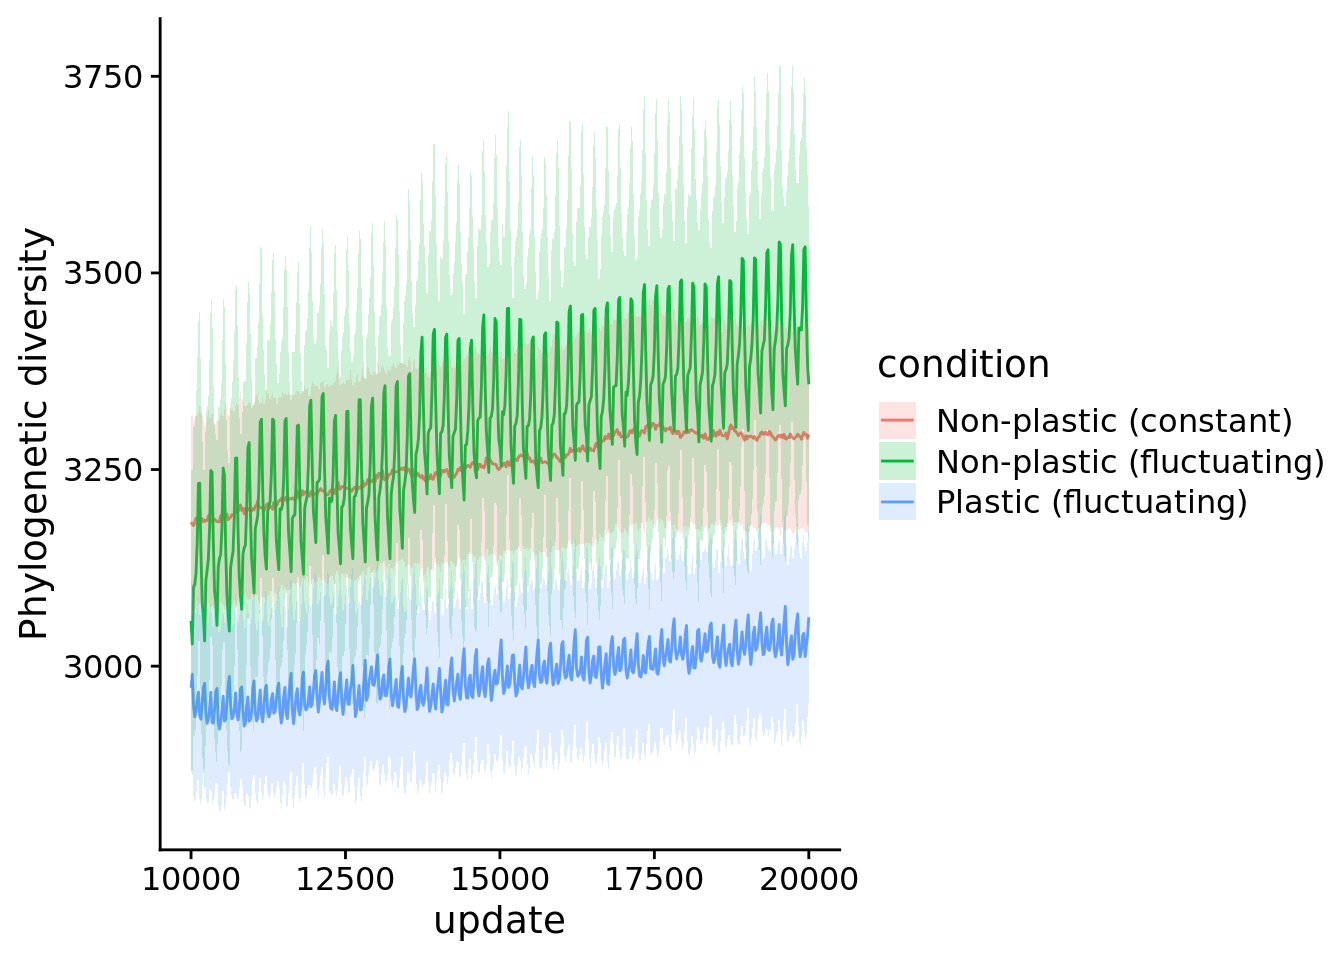
\includegraphics{supplemental-material_files/figure-latex/unnamed-chunk-24-1.pdf}

\begin{Shaded}
\begin{Highlighting}[]
\KeywordTok{kruskal.test}\NormalTok{(}
  \DataTypeTok{formula=}\NormalTok{dominant_lineage_trait_fidelity}\OperatorTok{~}\NormalTok{condition,}
  \DataTypeTok{data=}\NormalTok{summary_data}
\NormalTok{)}
\end{Highlighting}
\end{Shaded}

\begin{verbatim}
## 
##  Kruskal-Wallis rank sum test
## 
## data:  dominant_lineage_trait_fidelity by condition
## Kruskal-Wallis chi-squared = 189.62, df = 2, p-value < 2.2e-16
\end{verbatim}

\begin{Shaded}
\begin{Highlighting}[]
\KeywordTok{pairwise.wilcox.test}\NormalTok{(}
  \DataTypeTok{x=}\NormalTok{summary_data}\OperatorTok{$}\NormalTok{dominant_lineage_trait_fidelity,}
  \DataTypeTok{g=}\NormalTok{summary_data}\OperatorTok{$}\NormalTok{condition,}
  \DataTypeTok{p.adjust.method=}\StringTok{"bonferroni"}\NormalTok{,}
\NormalTok{)}
\end{Highlighting}
\end{Shaded}

\begin{verbatim}
## 
##  Pairwise comparisons using Wilcoxon rank sum test with continuity correction 
## 
## data:  summary_data$dominant_lineage_trait_fidelity and summary_data$condition 
## 
##         NON-PLASTIC PLASTIC
## PLASTIC < 2e-16     -      
## STATIC  < 2e-16     4.2e-06
## 
## P value adjustment method: bonferroni
\end{verbatim}

\begin{Shaded}
\begin{Highlighting}[]
\KeywordTok{paste}\NormalTok{(}
  \DataTypeTok{sep=}\StringTok{"; "}\NormalTok{,}
  \KeywordTok{paste0}\NormalTok{(}
    \StringTok{"PLASTIC median: "}\NormalTok{,}
    \KeywordTok{median}\NormalTok{(}\KeywordTok{filter}\NormalTok{(summary_data, condition}\OperatorTok{==}\StringTok{"PLASTIC"}\NormalTok{)}\OperatorTok{$}\NormalTok{dominant_lineage_trait_fidelity)}
\NormalTok{  ),}
  \KeywordTok{paste0}\NormalTok{(}
    \StringTok{"STATIC median: "}\NormalTok{,}
    \KeywordTok{median}\NormalTok{(}\KeywordTok{filter}\NormalTok{(summary_data, condition}\OperatorTok{==}\StringTok{"STATIC"}\NormalTok{)}\OperatorTok{$}\NormalTok{dominant_lineage_trait_fidelity)}
\NormalTok{  ),}
  \KeywordTok{paste0}\NormalTok{(}
    \StringTok{"NON-PLASTIC median: "}\NormalTok{,}
    \KeywordTok{median}\NormalTok{(}\KeywordTok{filter}\NormalTok{(summary_data, condition}\OperatorTok{==}\StringTok{"NON-PLASTIC"}\NormalTok{)}\OperatorTok{$}\NormalTok{dominant_lineage_trait_fidelity)}
\NormalTok{  )}
\NormalTok{)}
\end{Highlighting}
\end{Shaded}

\begin{verbatim}
## [1] "PLASTIC median: 0.999936666072028; STATIC median: 1; NON-PLASTIC median: 0.955255985436182"
\end{verbatim}

\begin{Shaded}
\begin{Highlighting}[]
\KeywordTok{print}\NormalTok{(}\StringTok{"Wilcox rank sum test statistics:"}\NormalTok{)}
\end{Highlighting}
\end{Shaded}

\begin{verbatim}
## [1] "Wilcox rank sum test statistics:"
\end{verbatim}

\begin{Shaded}
\begin{Highlighting}[]
\ControlFlowTok{for}\NormalTok{ (pair }\ControlFlowTok{in}\NormalTok{ pairwise_comparisons) \{}
\NormalTok{  pair_data <-}\StringTok{ }\KeywordTok{filter}\NormalTok{(summary_data, condition }\OperatorTok\StringTok{ }\NormalTok{pair)}
\NormalTok{  pair_data}\OperatorTok{$}\NormalTok{condition <-}\StringTok{ }\KeywordTok{as.factor}\NormalTok{(pair_data}\OperatorTok{$}\NormalTok{condition)}
\NormalTok{  wt <-}\StringTok{ }\KeywordTok{wilcox.test}\NormalTok{(}
    \DataTypeTok{formula=}\NormalTok{dominant_lineage_trait_fidelity}\OperatorTok{~}\NormalTok{condition,}
    \DataTypeTok{data=}\NormalTok{pair_data,}
    \DataTypeTok{exact=}\OtherTok{FALSE}\NormalTok{,}
    \DataTypeTok{paired=}\OtherTok{FALSE}
\NormalTok{  )}
  \KeywordTok{print}\NormalTok{(}\KeywordTok{paste0}\NormalTok{(pair[}\DecValTok{1}\NormalTok{], }\StringTok{"<-->"}\NormalTok{, pair[}\DecValTok{2}\NormalTok{], }\StringTok{": W="}\NormalTok{,wt}\OperatorTok{$}\NormalTok{statistic))}
\NormalTok{\}}
\end{Highlighting}
\end{Shaded}

\begin{verbatim}
## [1] "STATIC<-->NON-PLASTIC: W=0"
## [1] "STATIC<-->PLASTIC: W=1138.5"
## [1] "PLASTIC<-->NON-PLASTIC: W=0"
\end{verbatim}

\hypertarget{mutation-count}{%
\section{Mutation count}\label{mutation-count}}

\begin{Shaded}
\begin{Highlighting}[]
\CommentTok{# Compute manual labels for geom_signif}
\NormalTok{stat.test <-}\StringTok{ }\NormalTok{summary_data }\OperatorTok
\StringTok{  }\KeywordTok{wilcox_test}\NormalTok{(dominant_lineage_total_mut_cnt }\OperatorTok{~}\StringTok{ }\NormalTok{condition) }\OperatorTok
\StringTok{  }\KeywordTok{adjust_pvalue}\NormalTok{(}\DataTypeTok{method =} \StringTok{"bonferroni"}\NormalTok{) }\OperatorTok
\StringTok{  }\KeywordTok{add_significance}\NormalTok{() }\OperatorTok
\StringTok{  }\KeywordTok{add_xy_position}\NormalTok{(}\DataTypeTok{x=}\StringTok{"condition"}\NormalTok{,}\DataTypeTok{step.increase=}\DecValTok{1}\NormalTok{)}
\CommentTok{# Tweak y.position manually to account for scaled axis (edge case that triggers bad behavior in geom_signif)}
\NormalTok{stat.test}\OperatorTok{$}\NormalTok{manual_position <-}\StringTok{ }\KeywordTok{log10}\NormalTok{(stat.test}\OperatorTok{$}\NormalTok{y.position) }\OperatorTok{*}\StringTok{  }\KeywordTok{c}\NormalTok{(}\FloatTok{1.0}\NormalTok{,}\FloatTok{1.0}\NormalTok{,}\FloatTok{1.03}\NormalTok{) }\CommentTok{# c(1.0,1.0,1.01)}
\NormalTok{stat.test}\OperatorTok{$}\NormalTok{label <-}\StringTok{ }\KeywordTok{mapply}\NormalTok{(p_label,stat.test}\OperatorTok{$}\NormalTok{p.adj)}

\NormalTok{summary_data}\OperatorTok{$}\NormalTok{is_outlier <-}\StringTok{ }\KeywordTok{mapply}\NormalTok{(}
\NormalTok{  is_outlier,}
\NormalTok{  summary_data}\OperatorTok{$}\NormalTok{dominant_lineage_total_mut_cnt,}
\NormalTok{  summary_data}\OperatorTok{$}\NormalTok{condition,}
  \DataTypeTok{MoreArgs=}\KeywordTok{list}\NormalTok{(}\DataTypeTok{data=}\NormalTok{summary_data, }\DataTypeTok{column=}\StringTok{"dominant_lineage_total_mut_cnt"}\NormalTok{)}
\NormalTok{)}

\NormalTok{mutation_count_fig <-}\StringTok{ }\KeywordTok{ggplot}\NormalTok{(}
\NormalTok{    summary_data,}
    \KeywordTok{aes}\NormalTok{(}\DataTypeTok{x=}\NormalTok{condition, }\DataTypeTok{y=}\NormalTok{dominant_lineage_total_mut_cnt, }\DataTypeTok{fill=}\NormalTok{condition)}
\NormalTok{  ) }\OperatorTok{+}
\StringTok{  }\KeywordTok{geom_flat_violin}\NormalTok{(}
    \CommentTok{# data=filter(summary_data, !is_outlier),}
    \DataTypeTok{scale=}\StringTok{"width"}\NormalTok{,}
    \DataTypeTok{position =} \KeywordTok{position_nudge}\NormalTok{(}\DataTypeTok{x =} \FloatTok{.2}\NormalTok{, }\DataTypeTok{y =} \DecValTok{0}\NormalTok{),}
    \DataTypeTok{alpha =} \FloatTok{.8}
\NormalTok{  ) }\OperatorTok{+}
\StringTok{  }\KeywordTok{geom_point}\NormalTok{(}
    \DataTypeTok{mapping=}\KeywordTok{aes}\NormalTok{(}\DataTypeTok{color=}\NormalTok{condition),}
    \DataTypeTok{position =} \KeywordTok{position_jitter}\NormalTok{(}\DataTypeTok{width =} \FloatTok{.15}\NormalTok{),}
    \DataTypeTok{size =} \FloatTok{.5}\NormalTok{,}
    \DataTypeTok{alpha =} \FloatTok{0.8}
\NormalTok{  ) }\OperatorTok{+}
\StringTok{  }\KeywordTok{geom_boxplot}\NormalTok{(}
    \DataTypeTok{width =} \FloatTok{.1}\NormalTok{,}
    \DataTypeTok{outlier.shape =} \OtherTok{NA}\NormalTok{,}
    \DataTypeTok{alpha =} \FloatTok{0.5}
\NormalTok{  ) }\OperatorTok{+}
\StringTok{  }\KeywordTok{scale_x_discrete}\NormalTok{(}
    \DataTypeTok{name=}\StringTok{"Condition"}\NormalTok{,}
    \DataTypeTok{limits=}\NormalTok{condition_order,}
    \DataTypeTok{labels=}\NormalTok{condition_order}
\NormalTok{  ) }\OperatorTok{+}
\StringTok{  }\KeywordTok{scale_y_continuous}\NormalTok{(}
    \DataTypeTok{name=}\StringTok{"Mutation count (log scale)"}\NormalTok{,}
    \DataTypeTok{trans=}\KeywordTok{pseudo_log_trans}\NormalTok{(}\DataTypeTok{sigma =} \DecValTok{1}\NormalTok{, }\DataTypeTok{base =} \DecValTok{10}\NormalTok{),}
    \DataTypeTok{breaks=}\KeywordTok{c}\NormalTok{(}\DecValTok{0}\NormalTok{, }\DecValTok{10}\NormalTok{, }\DecValTok{100}\NormalTok{, }\DecValTok{1000}\NormalTok{, }\DecValTok{10000}\NormalTok{),}
    \DataTypeTok{limits=}\KeywordTok{c}\NormalTok{(}\OperatorTok{-}\DecValTok{1}\NormalTok{, }\DecValTok{35000}\NormalTok{)}
\NormalTok{  ) }\OperatorTok{+}
\StringTok{  }\KeywordTok{scale_fill_brewer}\NormalTok{(}
    \DataTypeTok{palette=}\NormalTok{cb_palette}
\NormalTok{  ) }\OperatorTok{+}
\StringTok{  }\KeywordTok{scale_color_brewer}\NormalTok{(}
    \DataTypeTok{palette=}\NormalTok{cb_palette}
\NormalTok{  ) }\OperatorTok{+}
\StringTok{  }\KeywordTok{labs}\NormalTok{(}
    \DataTypeTok{subtitle=}\KeywordTok{paste0}\NormalTok{(}
      \StringTok{"Kruskal-Wallis, "}\NormalTok{,}
      \KeywordTok{p_label}\NormalTok{(}\KeywordTok{signif}\NormalTok{(}\KeywordTok{kruskal.test}\NormalTok{(}\DataTypeTok{formula=}\NormalTok{dominant_lineage_total_mut_cnt}\OperatorTok{~}\NormalTok{condition, }\DataTypeTok{data=}\NormalTok{summary_data)}\OperatorTok{$}\NormalTok{p.value,}\DataTypeTok{digits=}\DecValTok{4}\NormalTok{))}
\NormalTok{    )}
\NormalTok{  ) }\OperatorTok{+}
\StringTok{  }\NormalTok{ggsignif}\OperatorTok{::}\KeywordTok{geom_signif}\NormalTok{(}
    \DataTypeTok{data=}\KeywordTok{filter}\NormalTok{(stat.test, p.adj }\OperatorTok{<=}\StringTok{ }\NormalTok{alpha),}
    \KeywordTok{aes}\NormalTok{(}\DataTypeTok{xmin=}\NormalTok{group1,}\DataTypeTok{xmax=}\NormalTok{group2,}\DataTypeTok{annotations=}\NormalTok{label,}\DataTypeTok{y_position=}\NormalTok{manual_position),}
    \DataTypeTok{manual=}\OtherTok{TRUE}\NormalTok{,}
    \DataTypeTok{inherit.aes=}\OtherTok{FALSE}
\NormalTok{  ) }\OperatorTok{+}
\StringTok{  }\KeywordTok{theme}\NormalTok{(}
    \DataTypeTok{legend.position=}\StringTok{"none"}
\NormalTok{  )}
\end{Highlighting}
\end{Shaded}

\begin{verbatim}
## Warning: Ignoring unknown aesthetics: xmin, xmax, annotations, y_position
\end{verbatim}

\begin{Shaded}
\begin{Highlighting}[]
\KeywordTok{ggsave}\NormalTok{(}
  \KeywordTok{paste0}\NormalTok{(working_directory, }\StringTok{"plots/"}\NormalTok{, }\StringTok{"mutation-accumulation.pdf"}\NormalTok{),}
  \DataTypeTok{width=}\DecValTok{5}\NormalTok{,}
  \DataTypeTok{height=}\DecValTok{4}
\NormalTok{)}
\NormalTok{mutation_count_fig}
\end{Highlighting}
\end{Shaded}

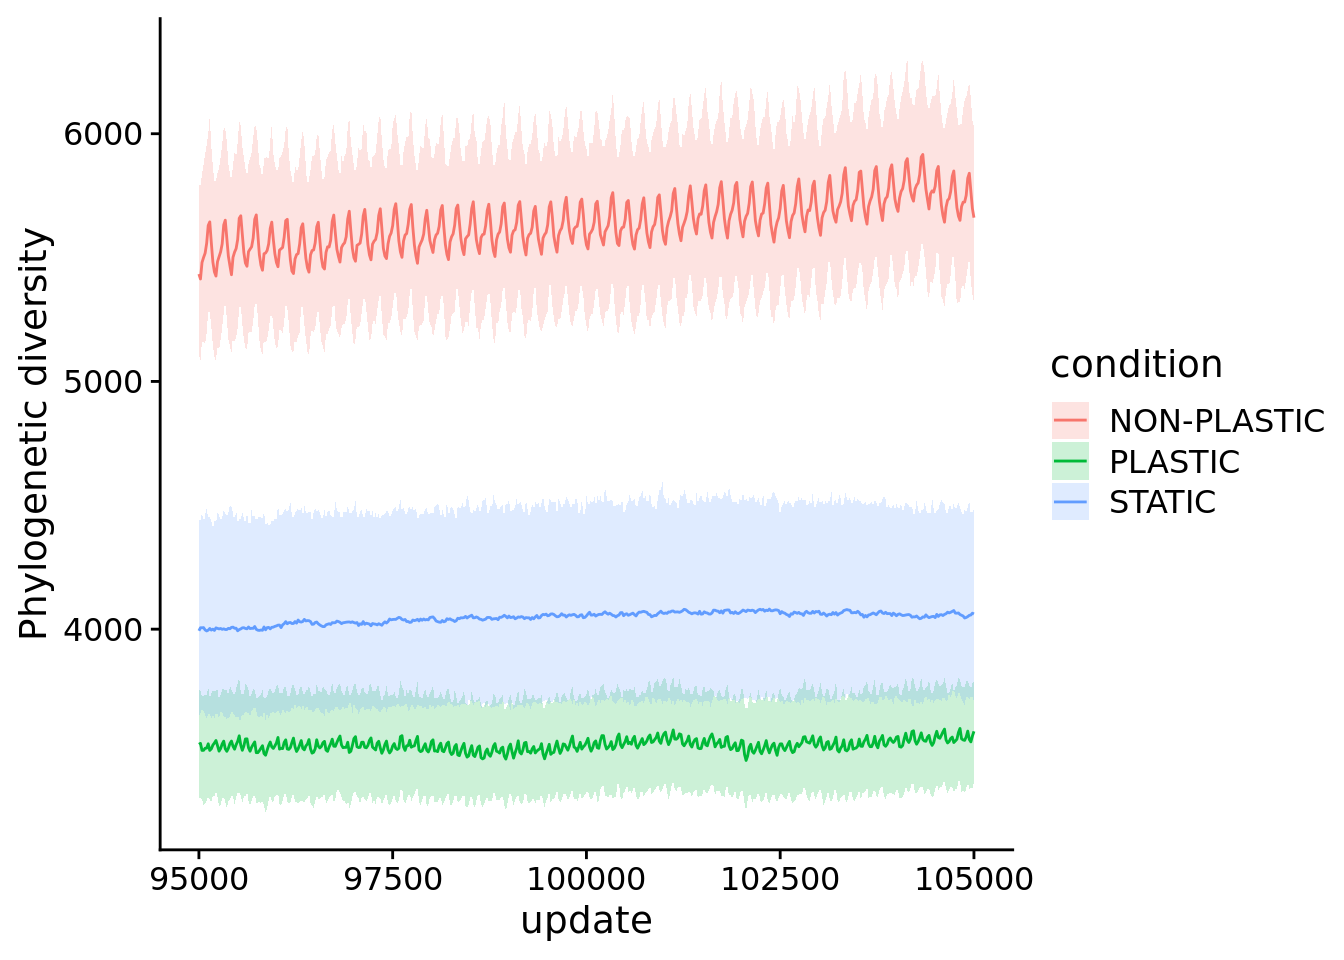
\includegraphics{supplemental-material_files/figure-latex/unnamed-chunk-26-1.pdf}

\begin{Shaded}
\begin{Highlighting}[]
\KeywordTok{kruskal.test}\NormalTok{(}
  \DataTypeTok{formula=}\NormalTok{dominant_lineage_total_mut_cnt}\OperatorTok{~}\NormalTok{condition,}
  \DataTypeTok{data=}\NormalTok{summary_data}
\NormalTok{)}
\end{Highlighting}
\end{Shaded}

\begin{verbatim}
## 
##  Kruskal-Wallis rank sum test
## 
## data:  dominant_lineage_total_mut_cnt by condition
## Kruskal-Wallis chi-squared = 179.33, df = 2, p-value < 2.2e-16
\end{verbatim}

\begin{Shaded}
\begin{Highlighting}[]
\KeywordTok{pairwise.wilcox.test}\NormalTok{(}
  \DataTypeTok{x=}\NormalTok{summary_data}\OperatorTok{$}\NormalTok{dominant_lineage_total_mut_cnt,}
  \DataTypeTok{g=}\NormalTok{summary_data}\OperatorTok{$}\NormalTok{condition,}
  \DataTypeTok{p.adjust.method=}\StringTok{"bonferroni"}\NormalTok{,}
\NormalTok{)}
\end{Highlighting}
\end{Shaded}

\begin{verbatim}
## 
##  Pairwise comparisons using Wilcoxon rank sum test with continuity correction 
## 
## data:  summary_data$dominant_lineage_total_mut_cnt and summary_data$condition 
## 
##         NON-PLASTIC PLASTIC
## PLASTIC <2e-16      -      
## STATIC  <2e-16      0.0019 
## 
## P value adjustment method: bonferroni
\end{verbatim}

\begin{Shaded}
\begin{Highlighting}[]
\KeywordTok{paste}\NormalTok{(}
  \DataTypeTok{sep=}\StringTok{"; "}\NormalTok{,}
  \KeywordTok{paste0}\NormalTok{(}
    \StringTok{"PLASTIC median: "}\NormalTok{,}
    \KeywordTok{median}\NormalTok{(}\KeywordTok{filter}\NormalTok{(summary_data, condition}\OperatorTok{==}\StringTok{"PLASTIC"}\NormalTok{)}\OperatorTok{$}\NormalTok{dominant_lineage_total_mut_cnt)}
\NormalTok{  ),}
  \KeywordTok{paste0}\NormalTok{(}
    \StringTok{"STATIC median: "}\NormalTok{,}
    \KeywordTok{median}\NormalTok{(}\KeywordTok{filter}\NormalTok{(summary_data, condition}\OperatorTok{==}\StringTok{"STATIC"}\NormalTok{)}\OperatorTok{$}\NormalTok{dominant_lineage_total_mut_cnt)}
\NormalTok{  ),}
  \KeywordTok{paste0}\NormalTok{(}
    \StringTok{"NON-PLASTIC median: "}\NormalTok{,}
    \KeywordTok{median}\NormalTok{(}\KeywordTok{filter}\NormalTok{(summary_data, condition}\OperatorTok{==}\StringTok{"NON-PLASTIC"}\NormalTok{)}\OperatorTok{$}\NormalTok{dominant_lineage_total_mut_cnt)}
\NormalTok{  )}
\NormalTok{)}
\end{Highlighting}
\end{Shaded}

\begin{verbatim}
## [1] "PLASTIC median: 998.5; STATIC median: 1100; NON-PLASTIC median: 4657.5"
\end{verbatim}

\begin{Shaded}
\begin{Highlighting}[]
\KeywordTok{print}\NormalTok{(}\StringTok{"Wilcox rank sum test statistics:"}\NormalTok{)}
\end{Highlighting}
\end{Shaded}

\begin{verbatim}
## [1] "Wilcox rank sum test statistics:"
\end{verbatim}

\begin{Shaded}
\begin{Highlighting}[]
\ControlFlowTok{for}\NormalTok{ (pair }\ControlFlowTok{in}\NormalTok{ pairwise_comparisons) \{}
\NormalTok{  pair_data <-}\StringTok{ }\KeywordTok{filter}\NormalTok{(summary_data, condition }\OperatorTok\StringTok{ }\NormalTok{pair)}
\NormalTok{  pair_data}\OperatorTok{$}\NormalTok{condition <-}\StringTok{ }\KeywordTok{as.factor}\NormalTok{(pair_data}\OperatorTok{$}\NormalTok{condition)}
\NormalTok{  wt <-}\StringTok{ }\KeywordTok{wilcox.test}\NormalTok{(}
    \DataTypeTok{formula=}\NormalTok{dominant_lineage_total_mut_cnt}\OperatorTok{~}\NormalTok{condition,}
    \DataTypeTok{data=}\NormalTok{pair_data,}
    \DataTypeTok{exact=}\OtherTok{FALSE}\NormalTok{,}
    \DataTypeTok{paired=}\OtherTok{FALSE}
\NormalTok{  )}
  \KeywordTok{print}\NormalTok{(}\KeywordTok{paste0}\NormalTok{(pair[}\DecValTok{1}\NormalTok{], }\StringTok{"<-->"}\NormalTok{, pair[}\DecValTok{2}\NormalTok{], }\StringTok{": W="}\NormalTok{,wt}\OperatorTok{$}\NormalTok{statistic))}
\NormalTok{\}}
\end{Highlighting}
\end{Shaded}

\begin{verbatim}
## [1] "STATIC<-->NON-PLASTIC: W=10000"
## [1] "STATIC<-->PLASTIC: W=1336.5"
## [1] "PLASTIC<-->NON-PLASTIC: W=4200"
\end{verbatim}

\hypertarget{mutation-count-normalized-by-generations-elapsed}{%
\subsection{Mutation count normalized by generations elapsed}\label{mutation-count-normalized-by-generations-elapsed}}

\begin{Shaded}
\begin{Highlighting}[]
\NormalTok{summary_data}\OperatorTok{$}\NormalTok{mutations_per_generation <-}\StringTok{ }\NormalTok{summary_data}\OperatorTok{$}\NormalTok{dominant_lineage_total_mut_cnt }\OperatorTok{/}\StringTok{ }\NormalTok{summary_data}\OperatorTok{$}\NormalTok{dominant_generation_born}

\KeywordTok{ggplot}\NormalTok{(summary_data, }\KeywordTok{aes}\NormalTok{(}\DataTypeTok{x=}\NormalTok{condition, }\DataTypeTok{y=}\NormalTok{mutations_per_generation, }\DataTypeTok{fill=}\NormalTok{condition)) }\OperatorTok{+}
\StringTok{  }\KeywordTok{geom_flat_violin}\NormalTok{(}
    \DataTypeTok{position =} \KeywordTok{position_nudge}\NormalTok{(}\DataTypeTok{x =} \FloatTok{.2}\NormalTok{, }\DataTypeTok{y =} \DecValTok{0}\NormalTok{),}
    \DataTypeTok{alpha =} \FloatTok{.8}
\NormalTok{  ) }\OperatorTok{+}
\StringTok{  }\KeywordTok{geom_point}\NormalTok{(}
    \DataTypeTok{mapping=}\KeywordTok{aes}\NormalTok{(}\DataTypeTok{color=}\NormalTok{condition),}
    \DataTypeTok{position =} \KeywordTok{position_jitter}\NormalTok{(}\DataTypeTok{width =} \FloatTok{.15}\NormalTok{),}
    \DataTypeTok{size =} \FloatTok{.5}\NormalTok{,}
    \DataTypeTok{alpha =} \FloatTok{0.8}
\NormalTok{  ) }\OperatorTok{+}
\StringTok{  }\KeywordTok{geom_boxplot}\NormalTok{(}
    \DataTypeTok{width =} \FloatTok{.1}\NormalTok{,}
    \DataTypeTok{outlier.shape =} \OtherTok{NA}\NormalTok{,}
    \DataTypeTok{alpha =} \FloatTok{0.5}
\NormalTok{  ) }\OperatorTok{+}
\StringTok{  }\KeywordTok{scale_x_discrete}\NormalTok{(}
    \DataTypeTok{name=}\StringTok{"Condition"}\NormalTok{,}
    \DataTypeTok{limits=}\NormalTok{condition_order}
\NormalTok{  ) }\OperatorTok{+}
\StringTok{  }\KeywordTok{ylab}\NormalTok{(}\StringTok{"Mutation count / generation"}\NormalTok{) }\OperatorTok{+}
\StringTok{  }\KeywordTok{scale_fill_brewer}\NormalTok{(}
    \DataTypeTok{palette=}\NormalTok{cb_palette}
\NormalTok{  ) }\OperatorTok{+}
\StringTok{  }\KeywordTok{scale_color_brewer}\NormalTok{(}
    \DataTypeTok{palette=}\NormalTok{cb_palette}
\NormalTok{  ) }\OperatorTok{+}
\StringTok{  }\KeywordTok{theme}\NormalTok{(}
    \DataTypeTok{legend.position=}\StringTok{"none"}
\NormalTok{  )}
\end{Highlighting}
\end{Shaded}

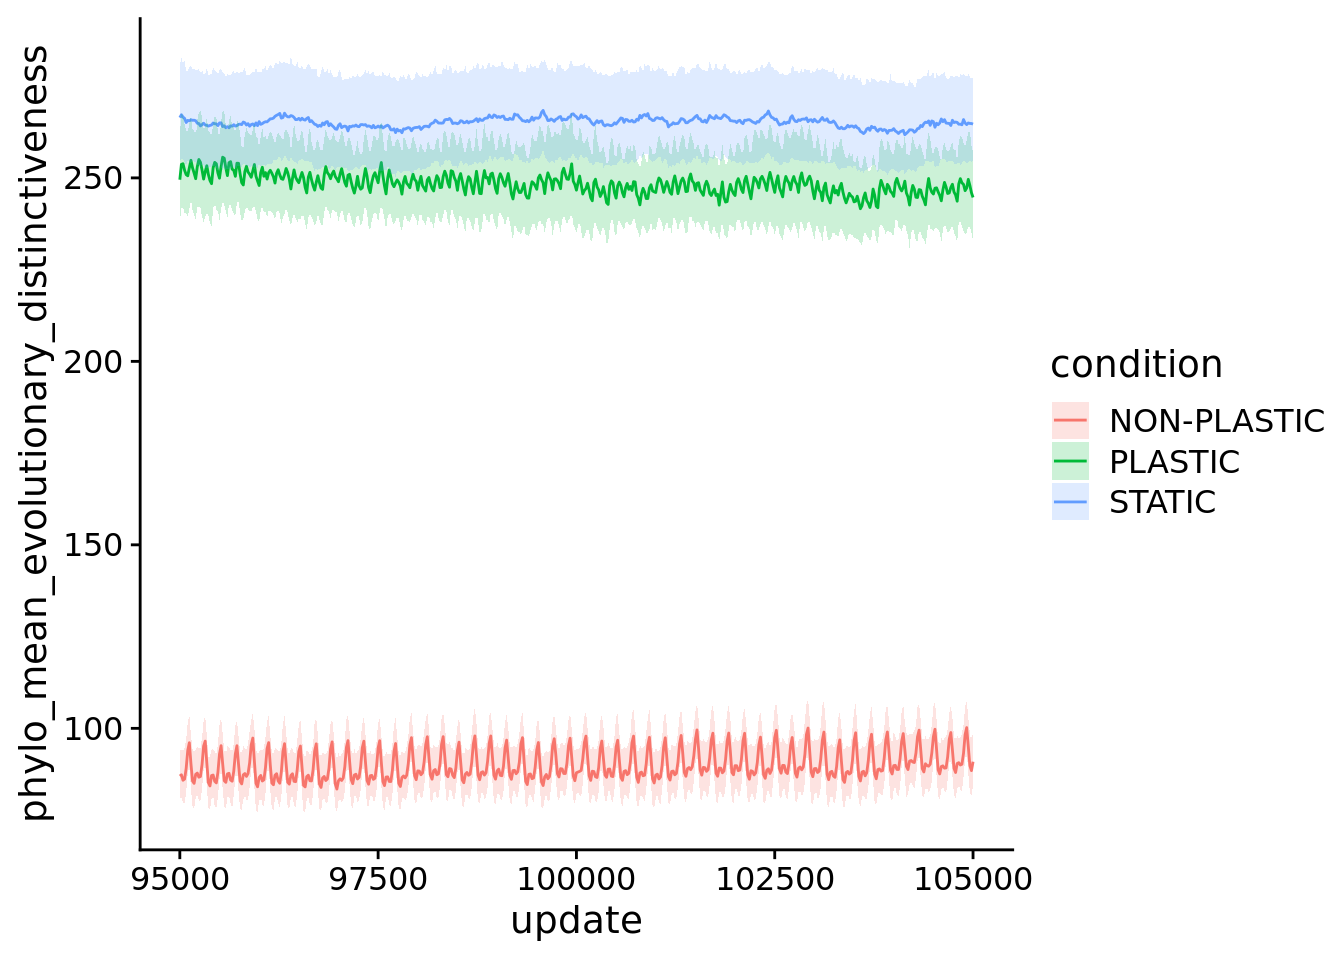
\includegraphics{supplemental-material_files/figure-latex/unnamed-chunk-28-1.pdf}

\begin{Shaded}
\begin{Highlighting}[]
\KeywordTok{kruskal.test}\NormalTok{(}
  \DataTypeTok{formula=}\NormalTok{mutations_per_generation}\OperatorTok{~}\NormalTok{condition,}
  \DataTypeTok{data=}\NormalTok{summary_data}
\NormalTok{)}
\end{Highlighting}
\end{Shaded}

\begin{verbatim}
## 
##  Kruskal-Wallis rank sum test
## 
## data:  mutations_per_generation by condition
## Kruskal-Wallis chi-squared = 180.11, df = 2, p-value < 2.2e-16
\end{verbatim}

\begin{Shaded}
\begin{Highlighting}[]
\KeywordTok{pairwise.wilcox.test}\NormalTok{(}
  \DataTypeTok{x=}\NormalTok{summary_data}\OperatorTok{$}\NormalTok{mutations_per_generation,}
  \DataTypeTok{g=}\NormalTok{summary_data}\OperatorTok{$}\NormalTok{condition,}
  \DataTypeTok{p.adjust.method=}\StringTok{"bonferroni"}\NormalTok{,}
\NormalTok{)}
\end{Highlighting}
\end{Shaded}

\begin{verbatim}
## 
##  Pairwise comparisons using Wilcoxon rank sum test with continuity correction 
## 
## data:  summary_data$mutations_per_generation and summary_data$condition 
## 
##         NON-PLASTIC PLASTIC
## PLASTIC <2e-16      -      
## STATIC  <2e-16      2e-04  
## 
## P value adjustment method: bonferroni
\end{verbatim}

\begin{Shaded}
\begin{Highlighting}[]
\KeywordTok{paste}\NormalTok{(}
  \DataTypeTok{sep=}\StringTok{"; "}\NormalTok{,}
  \KeywordTok{paste0}\NormalTok{(}
    \StringTok{"PLASTIC median: "}\NormalTok{,}
    \KeywordTok{median}\NormalTok{(}\KeywordTok{filter}\NormalTok{(summary_data, condition}\OperatorTok{==}\StringTok{"PLASTIC"}\NormalTok{)}\OperatorTok{$}\NormalTok{mutations_per_generation)}
\NormalTok{  ),}
  \KeywordTok{paste0}\NormalTok{(}
    \StringTok{"STATIC median: "}\NormalTok{,}
    \KeywordTok{median}\NormalTok{(}\KeywordTok{filter}\NormalTok{(summary_data, condition}\OperatorTok{==}\StringTok{"STATIC"}\NormalTok{)}\OperatorTok{$}\NormalTok{mutations_per_generation)}
\NormalTok{  ),}
  \KeywordTok{paste0}\NormalTok{(}
    \StringTok{"NON-PLASTIC median: "}\NormalTok{,}
    \KeywordTok{median}\NormalTok{(}\KeywordTok{filter}\NormalTok{(summary_data, condition}\OperatorTok{==}\StringTok{"NON-PLASTIC"}\NormalTok{)}\OperatorTok{$}\NormalTok{mutations_per_generation)}
\NormalTok{  )}
\NormalTok{)}
\end{Highlighting}
\end{Shaded}

\begin{verbatim}
## [1] "PLASTIC median: 0.0319267181456982; STATIC median: 0.0368157192941933; NON-PLASTIC median: 0.112804526786948"
\end{verbatim}

\begin{Shaded}
\begin{Highlighting}[]
\KeywordTok{print}\NormalTok{(}\StringTok{"Wilcox rank sum test statistics:"}\NormalTok{)}
\end{Highlighting}
\end{Shaded}

\begin{verbatim}
## [1] "Wilcox rank sum test statistics:"
\end{verbatim}

\begin{Shaded}
\begin{Highlighting}[]
\ControlFlowTok{for}\NormalTok{ (pair }\ControlFlowTok{in}\NormalTok{ pairwise_comparisons) \{}
\NormalTok{  pair_data <-}\StringTok{ }\KeywordTok{filter}\NormalTok{(summary_data, condition }\OperatorTok\StringTok{ }\NormalTok{pair)}
\NormalTok{  pair_data}\OperatorTok{$}\NormalTok{condition <-}\StringTok{ }\KeywordTok{as.factor}\NormalTok{(pair_data}\OperatorTok{$}\NormalTok{condition)}
\NormalTok{  wt <-}\StringTok{ }\KeywordTok{wilcox.test}\NormalTok{(}
    \DataTypeTok{formula=}\NormalTok{mutations_per_generation}\OperatorTok{~}\NormalTok{condition,}
    \DataTypeTok{data=}\NormalTok{pair_data,}
    \DataTypeTok{exact=}\OtherTok{FALSE}\NormalTok{,}
    \DataTypeTok{paired=}\OtherTok{FALSE}
\NormalTok{  )}
  \KeywordTok{print}\NormalTok{(}\KeywordTok{paste0}\NormalTok{(pair[}\DecValTok{1}\NormalTok{], }\StringTok{"<-->"}\NormalTok{, pair[}\DecValTok{2}\NormalTok{], }\StringTok{": W="}\NormalTok{,wt}\OperatorTok{$}\NormalTok{statistic))}
\NormalTok{\}}
\end{Highlighting}
\end{Shaded}

\begin{verbatim}
## [1] "STATIC<-->NON-PLASTIC: W=9987"
## [1] "STATIC<-->PLASTIC: W=1206"
## [1] "PLASTIC<-->NON-PLASTIC: W=4198"
\end{verbatim}

\hypertarget{genotypic-fidelity}{%
\section{Genotypic fidelity}\label{genotypic-fidelity}}

The frequency that an offspring's genotype is the same as a parent's genotype.

\begin{Shaded}
\begin{Highlighting}[]
\NormalTok{summary_data}\OperatorTok{$}\NormalTok{dominant_lineage_genotypic_fidelity <-}\StringTok{ }\NormalTok{(summary_data}\OperatorTok{$}\NormalTok{dominant_generation_born }\OperatorTok{-}\StringTok{ }\NormalTok{summary_data}\OperatorTok{$}\NormalTok{dominant_lineage_num_mut_steps) }\OperatorTok{/}\StringTok{ }\NormalTok{summary_data}\OperatorTok{$}\NormalTok{dominant_generation_born}

\CommentTok{# Compute manual labels for geom_signif}
\NormalTok{stat.test <-}\StringTok{ }\NormalTok{summary_data }\OperatorTok
\StringTok{  }\KeywordTok{wilcox_test}\NormalTok{(dominant_lineage_genotypic_fidelity }\OperatorTok{~}\StringTok{ }\NormalTok{condition) }\OperatorTok
\StringTok{  }\KeywordTok{adjust_pvalue}\NormalTok{(}\DataTypeTok{method =} \StringTok{"bonferroni"}\NormalTok{) }\OperatorTok
\StringTok{  }\KeywordTok{add_significance}\NormalTok{() }\OperatorTok
\StringTok{  }\KeywordTok{add_xy_position}\NormalTok{(}\DataTypeTok{x=}\StringTok{"condition"}\NormalTok{,}\DataTypeTok{step.increase=}\FloatTok{0.2}\NormalTok{)}
\CommentTok{# Tweak y.position manually to account for scaled axis (edge case that triggers bad behavior in geom_signif)}
\NormalTok{stat.test}\OperatorTok{$}\NormalTok{manual_position <-}\StringTok{ }\NormalTok{stat.test}\OperatorTok{$}\NormalTok{y.position }\OperatorTok{*}\StringTok{ }\KeywordTok{c}\NormalTok{(}\FloatTok{1.0}\NormalTok{,}\FloatTok{1.0}\NormalTok{,}\FloatTok{1.0}\NormalTok{)}
\NormalTok{stat.test}\OperatorTok{$}\NormalTok{label <-}\StringTok{ }\KeywordTok{mapply}\NormalTok{(p_label,stat.test}\OperatorTok{$}\NormalTok{p.adj)}

\NormalTok{genotypic_fidelity_fig <-}\StringTok{ }\KeywordTok{ggplot}\NormalTok{(}
\NormalTok{    summary_data,}
    \KeywordTok{aes}\NormalTok{(}\DataTypeTok{x=}\NormalTok{condition, }\DataTypeTok{y=}\NormalTok{dominant_lineage_genotypic_fidelity, }\DataTypeTok{fill=}\NormalTok{condition)}
\NormalTok{  ) }\OperatorTok{+}
\StringTok{  }\KeywordTok{geom_flat_violin}\NormalTok{(}
    \DataTypeTok{position =} \KeywordTok{position_nudge}\NormalTok{(}\DataTypeTok{x =} \FloatTok{.2}\NormalTok{, }\DataTypeTok{y =} \DecValTok{0}\NormalTok{),}
    \DataTypeTok{alpha =} \FloatTok{.8}
\NormalTok{  ) }\OperatorTok{+}
\StringTok{  }\KeywordTok{geom_point}\NormalTok{(}
    \DataTypeTok{mapping=}\KeywordTok{aes}\NormalTok{(}\DataTypeTok{color=}\NormalTok{condition),}
    \DataTypeTok{position =} \KeywordTok{position_jitter}\NormalTok{(}\DataTypeTok{width =} \FloatTok{.15}\NormalTok{),}
    \DataTypeTok{size =} \FloatTok{.5}\NormalTok{,}
    \DataTypeTok{alpha =} \FloatTok{0.8}
\NormalTok{  ) }\OperatorTok{+}
\StringTok{  }\KeywordTok{geom_boxplot}\NormalTok{(}
    \DataTypeTok{width =} \FloatTok{.1}\NormalTok{,}
    \DataTypeTok{outlier.shape =} \OtherTok{NA}\NormalTok{,}
    \DataTypeTok{alpha =} \FloatTok{0.5}
\NormalTok{  ) }\OperatorTok{+}
\StringTok{  }\KeywordTok{scale_x_discrete}\NormalTok{(}
    \DataTypeTok{name=}\StringTok{"Condition"}\NormalTok{,}
    \DataTypeTok{limits=}\NormalTok{condition_order,}
    \DataTypeTok{labels=}\NormalTok{condition_order}
\NormalTok{  ) }\OperatorTok{+}
\StringTok{  }\KeywordTok{scale_y_continuous}\NormalTok{(}
    \DataTypeTok{name=}\StringTok{"Genotypic fidelity"}\NormalTok{,}
    \DataTypeTok{limits=}\KeywordTok{c}\NormalTok{(}\FloatTok{0.85}\NormalTok{, }\FloatTok{1.01}\NormalTok{),}
    \DataTypeTok{breaks=}\KeywordTok{c}\NormalTok{(}\FloatTok{0.85}\NormalTok{, }\FloatTok{0.90}\NormalTok{, }\FloatTok{0.95}\NormalTok{, }\FloatTok{1.0}\NormalTok{) }\CommentTok{#seq(0.85, 1.0, 0.02)}
\NormalTok{  ) }\OperatorTok{+}
\StringTok{  }\KeywordTok{scale_fill_brewer}\NormalTok{(}
    \DataTypeTok{palette=}\NormalTok{cb_palette}
\NormalTok{  ) }\OperatorTok{+}
\StringTok{  }\KeywordTok{scale_color_brewer}\NormalTok{(}
    \DataTypeTok{palette=}\NormalTok{cb_palette}
\NormalTok{  ) }\OperatorTok{+}
\StringTok{  }\CommentTok{# coord_flip() +}
\StringTok{  }\KeywordTok{labs}\NormalTok{(}
    \DataTypeTok{subtitle=}\KeywordTok{paste0}\NormalTok{(}
      \StringTok{"Kruskal-Wallis, "}\NormalTok{,}
      \KeywordTok{p_label}\NormalTok{(}\KeywordTok{signif}\NormalTok{(}\KeywordTok{kruskal.test}\NormalTok{(}\DataTypeTok{formula=}\NormalTok{dominant_lineage_genotypic_fidelity}\OperatorTok{~}\NormalTok{condition, }\DataTypeTok{data=}\NormalTok{summary_data)}\OperatorTok{$}\NormalTok{p.value,}\DataTypeTok{digits=}\DecValTok{4}\NormalTok{))}
\NormalTok{    )}
\NormalTok{  ) }\OperatorTok{+}
\StringTok{  }\NormalTok{ggsignif}\OperatorTok{::}\KeywordTok{geom_signif}\NormalTok{(}
    \DataTypeTok{data=}\KeywordTok{filter}\NormalTok{(stat.test, p.adj }\OperatorTok{<=}\StringTok{ }\NormalTok{alpha),}
    \KeywordTok{aes}\NormalTok{(}\DataTypeTok{xmin=}\NormalTok{group1,}\DataTypeTok{xmax=}\NormalTok{group2,}\DataTypeTok{annotations=}\NormalTok{label,}\DataTypeTok{y_position=}\NormalTok{manual_position),}
    \DataTypeTok{manual=}\OtherTok{TRUE}\NormalTok{,}
    \DataTypeTok{inherit.aes=}\OtherTok{FALSE}
\NormalTok{  ) }\OperatorTok{+}
\StringTok{  }\KeywordTok{theme}\NormalTok{(}
    \DataTypeTok{legend.position=}\StringTok{"none"}
\NormalTok{  )}
\end{Highlighting}
\end{Shaded}

\begin{verbatim}
## Warning: Ignoring unknown aesthetics: xmin, xmax, annotations, y_position
\end{verbatim}

\begin{Shaded}
\begin{Highlighting}[]
\KeywordTok{ggsave}\NormalTok{(}
  \KeywordTok{paste0}\NormalTok{(working_directory, }\StringTok{"plots/"}\NormalTok{, }\StringTok{"genotypic-fidelity.pdf"}\NormalTok{),}
  \DataTypeTok{width=}\DecValTok{5}\NormalTok{,}
  \DataTypeTok{height=}\DecValTok{4}
\NormalTok{)}
\NormalTok{genotypic_fidelity_fig}
\end{Highlighting}
\end{Shaded}

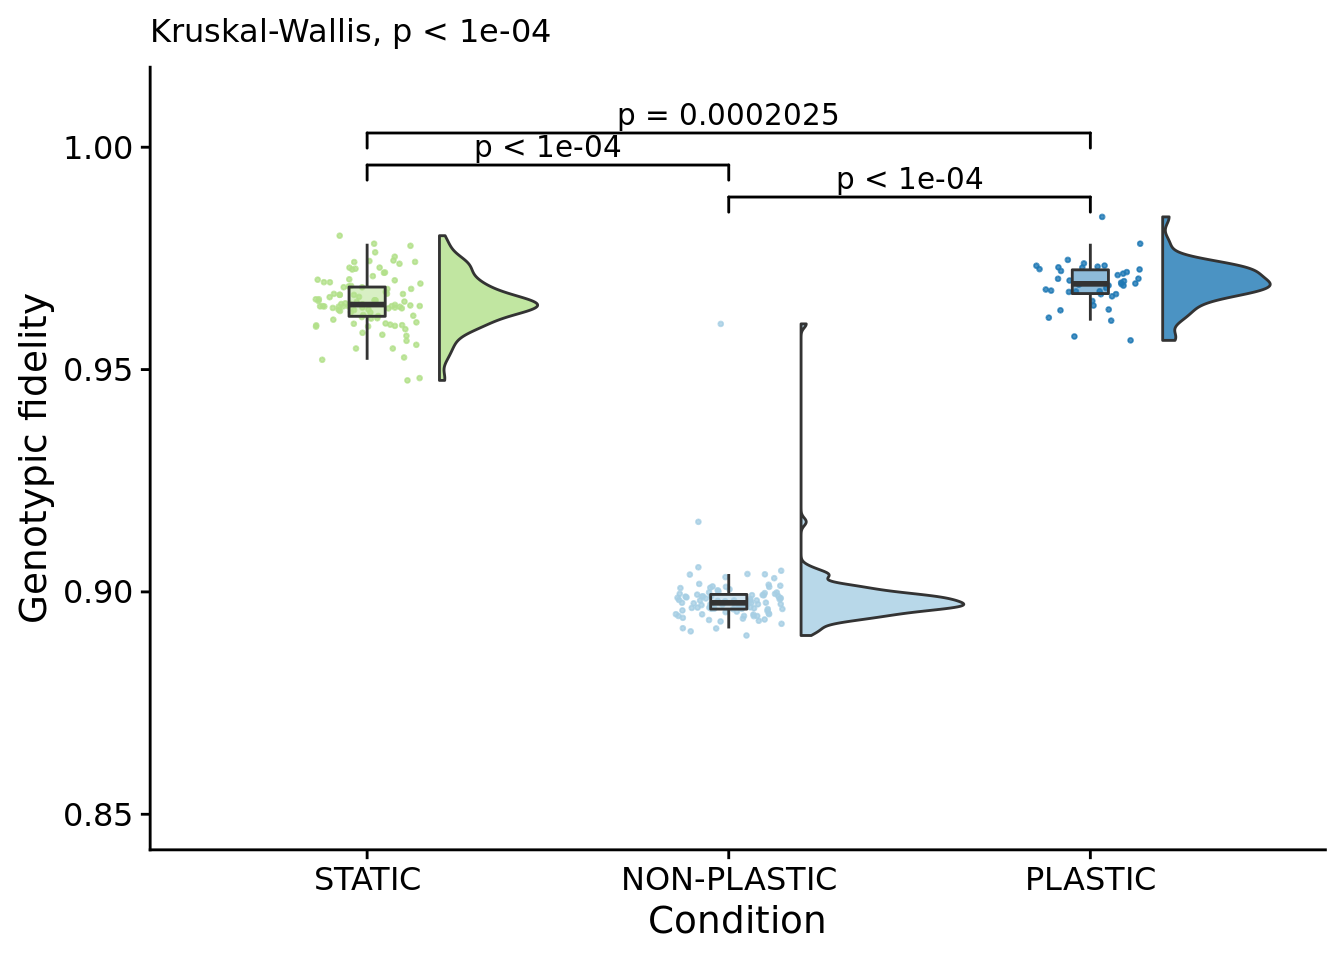
\includegraphics{supplemental-material_files/figure-latex/unnamed-chunk-30-1.pdf}

\begin{Shaded}
\begin{Highlighting}[]
\KeywordTok{kruskal.test}\NormalTok{(}
  \DataTypeTok{formula=}\NormalTok{dominant_lineage_genotypic_fidelity}\OperatorTok{~}\NormalTok{condition,}
  \DataTypeTok{data=}\NormalTok{summary_data}
\NormalTok{)}
\end{Highlighting}
\end{Shaded}

\begin{verbatim}
## 
##  Kruskal-Wallis rank sum test
## 
## data:  dominant_lineage_genotypic_fidelity by condition
## Kruskal-Wallis chi-squared = 179.86, df = 2, p-value < 2.2e-16
\end{verbatim}

\begin{Shaded}
\begin{Highlighting}[]
\KeywordTok{pairwise.wilcox.test}\NormalTok{(}
  \DataTypeTok{x=}\NormalTok{summary_data}\OperatorTok{$}\NormalTok{dominant_lineage_genotypic_fidelity,}
  \DataTypeTok{g=}\NormalTok{summary_data}\OperatorTok{$}\NormalTok{condition,}
  \DataTypeTok{p.adjust.method=}\StringTok{"bonferroni"}\NormalTok{,}
\NormalTok{)}
\end{Highlighting}
\end{Shaded}

\begin{verbatim}
## 
##  Pairwise comparisons using Wilcoxon rank sum test with continuity correction 
## 
## data:  summary_data$dominant_lineage_genotypic_fidelity and summary_data$condition 
## 
##         NON-PLASTIC PLASTIC
## PLASTIC <2e-16      -      
## STATIC  <2e-16      2e-04  
## 
## P value adjustment method: bonferroni
\end{verbatim}

\begin{Shaded}
\begin{Highlighting}[]
\KeywordTok{paste}\NormalTok{(}
  \DataTypeTok{sep=}\StringTok{"; "}\NormalTok{,}
  \KeywordTok{paste0}\NormalTok{(}
    \StringTok{"PLASTIC median: "}\NormalTok{,}
    \KeywordTok{median}\NormalTok{(}\KeywordTok{filter}\NormalTok{(summary_data, condition}\OperatorTok{==}\StringTok{"PLASTIC"}\NormalTok{)}\OperatorTok{$}\NormalTok{dominant_lineage_genotypic_fidelity)}
\NormalTok{  ),}
  \KeywordTok{paste0}\NormalTok{(}
    \StringTok{"STATIC median: "}\NormalTok{,}
    \KeywordTok{median}\NormalTok{(}\KeywordTok{filter}\NormalTok{(summary_data, condition}\OperatorTok{==}\StringTok{"STATIC"}\NormalTok{)}\OperatorTok{$}\NormalTok{dominant_lineage_genotypic_fidelity)}
\NormalTok{  ),}
  \KeywordTok{paste0}\NormalTok{(}
    \StringTok{"NON-PLASTIC median: "}\NormalTok{,}
    \KeywordTok{median}\NormalTok{(}\KeywordTok{filter}\NormalTok{(summary_data, condition}\OperatorTok{==}\StringTok{"NON-PLASTIC"}\NormalTok{)}\OperatorTok{$}\NormalTok{dominant_lineage_genotypic_fidelity)}
\NormalTok{  )}
\NormalTok{)}
\end{Highlighting}
\end{Shaded}

\begin{verbatim}
## [1] "PLASTIC median: 0.969286906891951; STATIC median: 0.964620594632577; NON-PLASTIC median: 0.89754902563783"
\end{verbatim}

\begin{Shaded}
\begin{Highlighting}[]
\KeywordTok{print}\NormalTok{(}\StringTok{"Wilcox rank sum test statistics:"}\NormalTok{)}
\end{Highlighting}
\end{Shaded}

\begin{verbatim}
## [1] "Wilcox rank sum test statistics:"
\end{verbatim}

\begin{Shaded}
\begin{Highlighting}[]
\ControlFlowTok{for}\NormalTok{ (pair }\ControlFlowTok{in}\NormalTok{ pairwise_comparisons) \{}
\NormalTok{  pair_data <-}\StringTok{ }\KeywordTok{filter}\NormalTok{(summary_data, condition }\OperatorTok\StringTok{ }\NormalTok{pair)}
\NormalTok{  pair_data}\OperatorTok{$}\NormalTok{condition <-}\StringTok{ }\KeywordTok{as.factor}\NormalTok{(pair_data}\OperatorTok{$}\NormalTok{condition)}
\NormalTok{  wt <-}\StringTok{ }\KeywordTok{wilcox.test}\NormalTok{(}
    \DataTypeTok{formula=}\NormalTok{dominant_lineage_genotypic_fidelity}\OperatorTok{~}\NormalTok{condition,}
    \DataTypeTok{data=}\NormalTok{pair_data,}
    \DataTypeTok{exact=}\OtherTok{FALSE}\NormalTok{,}
    \DataTypeTok{paired=}\OtherTok{FALSE}
\NormalTok{  )}
  \KeywordTok{print}\NormalTok{(}\KeywordTok{paste0}\NormalTok{(pair[}\DecValTok{1}\NormalTok{], }\StringTok{"<-->"}\NormalTok{, pair[}\DecValTok{2}\NormalTok{], }\StringTok{": W="}\NormalTok{,wt}\OperatorTok{$}\NormalTok{statistic))}
\NormalTok{\}}
\end{Highlighting}
\end{Shaded}

\begin{verbatim}
## [1] "STATIC<-->NON-PLASTIC: W=18"
## [1] "STATIC<-->PLASTIC: W=2992"
## [1] "PLASTIC<-->NON-PLASTIC: W=2"
\end{verbatim}

\hypertarget{characterizing-variation-along-dominant-lineages}{%
\section{Characterizing variation along dominant lineages}\label{characterizing-variation-along-dominant-lineages}}

\hypertarget{mutational-instability}{%
\subsection{Mutational instability}\label{mutational-instability}}

\begin{Shaded}
\begin{Highlighting}[]
\NormalTok{summary_data}\OperatorTok{$}\NormalTok{frac_phenotype_changing_mut_steps <-}\StringTok{ }\NormalTok{summary_data}\OperatorTok{$}\NormalTok{dominant_lineage_num_mut_steps_that_change_aggregate_phenotype }\OperatorTok{/}\StringTok{ }\NormalTok{summary_data}\OperatorTok{$}\NormalTok{dominant_lineage_num_mut_steps}
\NormalTok{summary_data}\OperatorTok{$}\NormalTok{frac_phenotype_stable_mut_steps <-}\StringTok{ }\DecValTok{1} \OperatorTok{-}\StringTok{ }\NormalTok{summary_data}\OperatorTok{$}\NormalTok{frac_phenotype_changing_mut_steps}

\CommentTok{# Compute manual labels for geom_signif}
\NormalTok{stat.test <-}\StringTok{ }\NormalTok{summary_data }\OperatorTok
\StringTok{  }\KeywordTok{wilcox_test}\NormalTok{(frac_phenotype_changing_mut_steps }\OperatorTok{~}\StringTok{ }\NormalTok{condition) }\OperatorTok
\StringTok{  }\KeywordTok{adjust_pvalue}\NormalTok{(}\DataTypeTok{method =} \StringTok{"bonferroni"}\NormalTok{) }\OperatorTok
\StringTok{  }\KeywordTok{add_significance}\NormalTok{() }\OperatorTok
\StringTok{  }\KeywordTok{add_xy_position}\NormalTok{(}\DataTypeTok{x=}\StringTok{"condition"}\NormalTok{,}\DataTypeTok{step.increase=}\FloatTok{0.2}\NormalTok{)}
\CommentTok{# Tweak y.position manually to account for scaled axis (edge case that triggers bad behavior in geom_signif)}
\NormalTok{stat.test}\OperatorTok{$}\NormalTok{manual_position <-}\StringTok{ }\NormalTok{stat.test}\OperatorTok{$}\NormalTok{y.position }\CommentTok{#* c(1.0,1.0,1.0)}
\NormalTok{stat.test}\OperatorTok{$}\NormalTok{label <-}\StringTok{ }\KeywordTok{mapply}\NormalTok{(p_label,stat.test}\OperatorTok{$}\NormalTok{p.adj)}

\KeywordTok{ggplot}\NormalTok{(summary_data, }\KeywordTok{aes}\NormalTok{(}\DataTypeTok{x=}\NormalTok{condition, }\DataTypeTok{y=}\NormalTok{frac_phenotype_changing_mut_steps, }\DataTypeTok{fill=}\NormalTok{condition)) }\OperatorTok{+}
\StringTok{  }\KeywordTok{geom_flat_violin}\NormalTok{(}
    \DataTypeTok{position =} \KeywordTok{position_nudge}\NormalTok{(}\DataTypeTok{x =} \FloatTok{.2}\NormalTok{, }\DataTypeTok{y =} \DecValTok{0}\NormalTok{),}
    \DataTypeTok{alpha =} \FloatTok{.8}
\NormalTok{  ) }\OperatorTok{+}
\StringTok{  }\KeywordTok{geom_point}\NormalTok{(}
    \DataTypeTok{mapping=}\KeywordTok{aes}\NormalTok{(}\DataTypeTok{color=}\NormalTok{condition),}
    \DataTypeTok{position =} \KeywordTok{position_jitter}\NormalTok{(}\DataTypeTok{width =} \FloatTok{.15}\NormalTok{),}
    \DataTypeTok{size =} \FloatTok{.5}\NormalTok{,}
    \DataTypeTok{alpha =} \FloatTok{0.8}
\NormalTok{  ) }\OperatorTok{+}
\StringTok{  }\KeywordTok{geom_boxplot}\NormalTok{(}
    \DataTypeTok{width =} \FloatTok{.1}\NormalTok{,}
    \DataTypeTok{outlier.shape =} \OtherTok{NA}\NormalTok{,}
    \DataTypeTok{alpha =} \FloatTok{0.5}
\NormalTok{  ) }\OperatorTok{+}
\StringTok{  }\KeywordTok{scale_x_discrete}\NormalTok{(}
    \DataTypeTok{name=}\StringTok{"Condition"}\NormalTok{,}
    \DataTypeTok{limits=}\NormalTok{condition_order}
\NormalTok{  ) }\OperatorTok{+}
\StringTok{  }\KeywordTok{ylab}\NormalTok{(}\StringTok{"Mutational instability"}\NormalTok{) }\OperatorTok{+}
\StringTok{  }\KeywordTok{scale_fill_brewer}\NormalTok{(}
    \DataTypeTok{palette=}\NormalTok{cb_palette}
\NormalTok{  ) }\OperatorTok{+}
\StringTok{  }\KeywordTok{scale_color_brewer}\NormalTok{(}
    \DataTypeTok{palette=}\NormalTok{cb_palette}
\NormalTok{  ) }\OperatorTok{+}
\StringTok{  }\CommentTok{# coord_flip() +}
\StringTok{  }\KeywordTok{labs}\NormalTok{(}
    \DataTypeTok{subtitle=}\KeywordTok{paste0}\NormalTok{(}
      \StringTok{"Kruskal-Wallis, "}\NormalTok{,}
      \KeywordTok{p_label}\NormalTok{(}\KeywordTok{signif}\NormalTok{(}\KeywordTok{kruskal.test}\NormalTok{(}\DataTypeTok{formula=}\NormalTok{frac_phenotype_changing_mut_steps}\OperatorTok{~}\NormalTok{condition, }\DataTypeTok{data=}\NormalTok{summary_data)}\OperatorTok{$}\NormalTok{p.value,}\DataTypeTok{digits=}\DecValTok{4}\NormalTok{))}
\NormalTok{    )}
\NormalTok{  ) }\OperatorTok{+}
\StringTok{  }\NormalTok{ggsignif}\OperatorTok{::}\KeywordTok{geom_signif}\NormalTok{(}
    \DataTypeTok{data=}\KeywordTok{filter}\NormalTok{(stat.test, p.adj }\OperatorTok{<=}\StringTok{ }\NormalTok{alpha),}
    \KeywordTok{aes}\NormalTok{(}\DataTypeTok{xmin=}\NormalTok{group1,}\DataTypeTok{xmax=}\NormalTok{group2,}\DataTypeTok{annotations=}\NormalTok{label,}\DataTypeTok{y_position=}\NormalTok{manual_position),}
    \DataTypeTok{manual=}\OtherTok{TRUE}\NormalTok{,}
    \DataTypeTok{inherit.aes=}\OtherTok{FALSE}
\NormalTok{  ) }\OperatorTok{+}
\StringTok{  }\KeywordTok{theme}\NormalTok{(}
    \DataTypeTok{legend.position=}\StringTok{"none"}
\NormalTok{  )}
\end{Highlighting}
\end{Shaded}

\begin{verbatim}
## Warning: Ignoring unknown aesthetics: xmin, xmax, annotations, y_position
\end{verbatim}

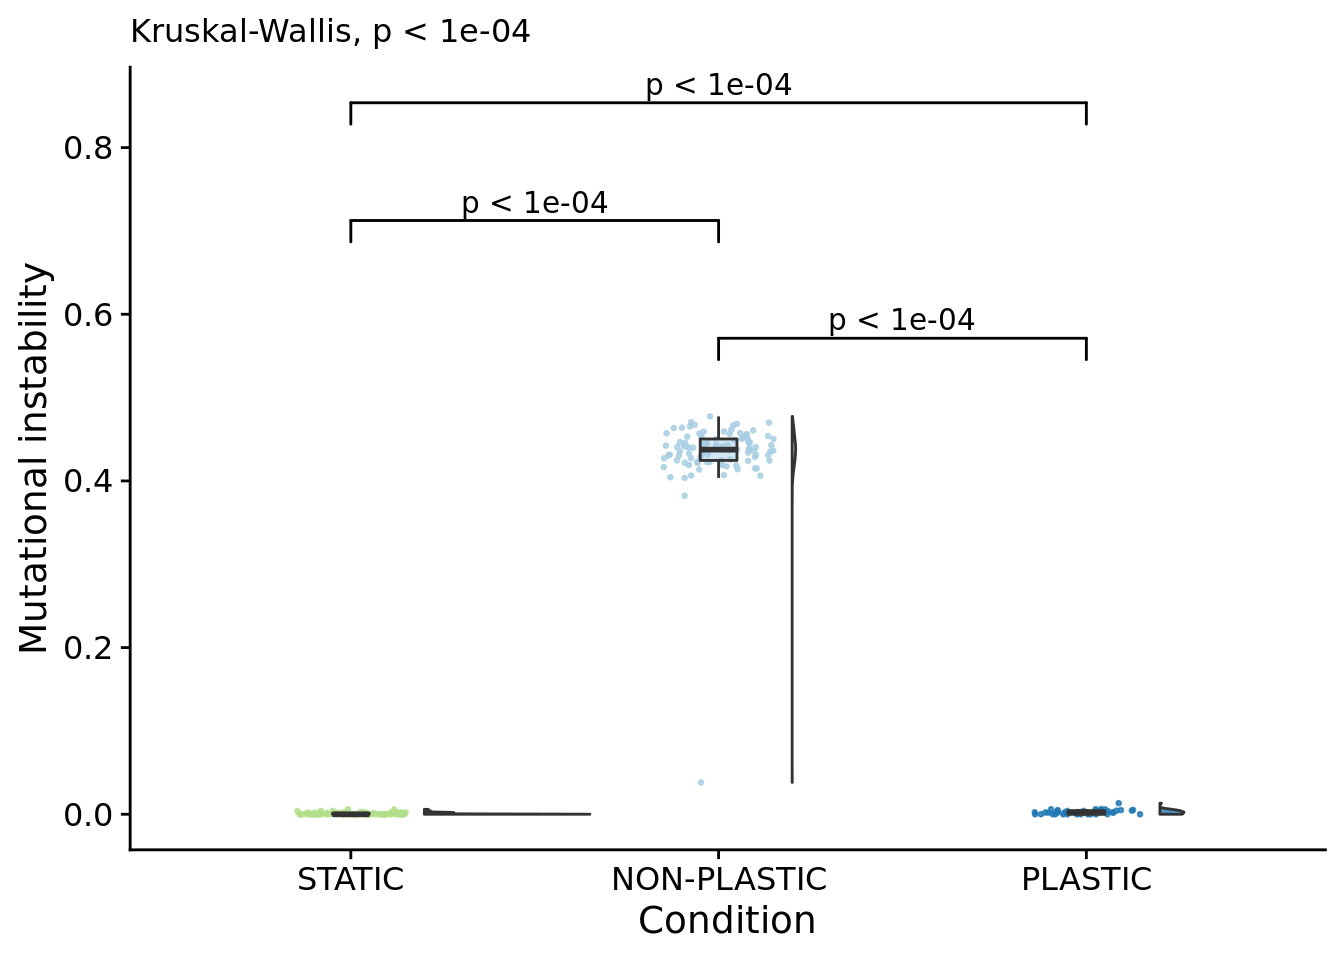
\includegraphics{supplemental-material_files/figure-latex/unnamed-chunk-32-1.pdf}

\begin{Shaded}
\begin{Highlighting}[]
\KeywordTok{ggsave}\NormalTok{(}\KeywordTok{paste0}\NormalTok{(working_directory, }\StringTok{"plots/"}\NormalTok{, }\StringTok{"frac_phenotype_changing_mutational_steps.png"}\NormalTok{))}
\end{Highlighting}
\end{Shaded}

\begin{verbatim}
## Saving 6.5 x 4.5 in image
\end{verbatim}

\begin{Shaded}
\begin{Highlighting}[]
\KeywordTok{kruskal.test}\NormalTok{(}
  \DataTypeTok{formula=}\NormalTok{frac_phenotype_changing_mut_steps}\OperatorTok{~}\NormalTok{condition,}
  \DataTypeTok{data=}\NormalTok{summary_data}
\NormalTok{)}
\end{Highlighting}
\end{Shaded}

\begin{verbatim}
## 
##  Kruskal-Wallis rank sum test
## 
## data:  frac_phenotype_changing_mut_steps by condition
## Kruskal-Wallis chi-squared = 191.23, df = 2, p-value < 2.2e-16
\end{verbatim}

\begin{Shaded}
\begin{Highlighting}[]
\KeywordTok{pairwise.wilcox.test}\NormalTok{(}
  \DataTypeTok{x=}\NormalTok{summary_data}\OperatorTok{$}\NormalTok{frac_phenotype_changing_mut_steps,}
  \DataTypeTok{g=}\NormalTok{summary_data}\OperatorTok{$}\NormalTok{condition,}
  \DataTypeTok{p.adjust.method=}\StringTok{"bonferroni"}\NormalTok{,}
\NormalTok{)}
\end{Highlighting}
\end{Shaded}

\begin{verbatim}
## 
##  Pairwise comparisons using Wilcoxon rank sum test with continuity correction 
## 
## data:  summary_data$frac_phenotype_changing_mut_steps and summary_data$condition 
## 
##         NON-PLASTIC PLASTIC
## PLASTIC < 2e-16     -      
## STATIC  < 2e-16     2.3e-07
## 
## P value adjustment method: bonferroni
\end{verbatim}

\begin{Shaded}
\begin{Highlighting}[]
\KeywordTok{paste}\NormalTok{(}
  \DataTypeTok{sep=}\StringTok{"; "}\NormalTok{,}
  \KeywordTok{paste0}\NormalTok{(}
    \StringTok{"PLASTIC median: "}\NormalTok{,}
    \KeywordTok{median}\NormalTok{(}\KeywordTok{filter}\NormalTok{(summary_data, condition}\OperatorTok{==}\StringTok{"PLASTIC"}\NormalTok{)}\OperatorTok{$}\NormalTok{frac_phenotype_changing_mut_steps)}
\NormalTok{  ),}
  \KeywordTok{paste0}\NormalTok{(}
    \StringTok{"STATIC median: "}\NormalTok{,}
    \KeywordTok{median}\NormalTok{(}\KeywordTok{filter}\NormalTok{(summary_data, condition}\OperatorTok{==}\StringTok{"STATIC"}\NormalTok{)}\OperatorTok{$}\NormalTok{frac_phenotype_changing_mut_steps)}
\NormalTok{  ),}
  \KeywordTok{paste0}\NormalTok{(}
    \StringTok{"NON-PLASTIC median: "}\NormalTok{,}
    \KeywordTok{median}\NormalTok{(}\KeywordTok{filter}\NormalTok{(summary_data, condition}\OperatorTok{==}\StringTok{"NON-PLASTIC"}\NormalTok{)}\OperatorTok{$}\NormalTok{frac_phenotype_changing_mut_steps)}
\NormalTok{  )}
\NormalTok{)}
\end{Highlighting}
\end{Shaded}

\begin{verbatim}
## [1] "PLASTIC median: 0.00224941742616098; STATIC median: 0; NON-PLASTIC median: 0.437583018324547"
\end{verbatim}

\begin{Shaded}
\begin{Highlighting}[]
\KeywordTok{print}\NormalTok{(}\StringTok{"Wilcox rank sum test statistics:"}\NormalTok{)}
\end{Highlighting}
\end{Shaded}

\begin{verbatim}
## [1] "Wilcox rank sum test statistics:"
\end{verbatim}

\begin{Shaded}
\begin{Highlighting}[]
\ControlFlowTok{for}\NormalTok{ (pair }\ControlFlowTok{in}\NormalTok{ pairwise_comparisons) \{}
\NormalTok{  pair_data <-}\StringTok{ }\KeywordTok{filter}\NormalTok{(summary_data, condition }\OperatorTok\StringTok{ }\NormalTok{pair)}
\NormalTok{  pair_data}\OperatorTok{$}\NormalTok{condition <-}\StringTok{ }\KeywordTok{as.factor}\NormalTok{(pair_data}\OperatorTok{$}\NormalTok{condition)}
\NormalTok{  wt <-}\StringTok{ }\KeywordTok{wilcox.test}\NormalTok{(}
    \DataTypeTok{formula=}\NormalTok{frac_phenotype_changing_mut_steps}\OperatorTok{~}\NormalTok{condition,}
    \DataTypeTok{data=}\NormalTok{pair_data,}
    \DataTypeTok{exact=}\OtherTok{FALSE}\NormalTok{,}
    \DataTypeTok{paired=}\OtherTok{FALSE}
\NormalTok{  )}
  \KeywordTok{print}\NormalTok{(}\KeywordTok{paste0}\NormalTok{(pair[}\DecValTok{1}\NormalTok{], }\StringTok{"<-->"}\NormalTok{, pair[}\DecValTok{2}\NormalTok{], }\StringTok{": W="}\NormalTok{,wt}\OperatorTok{$}\NormalTok{statistic))}
\NormalTok{\}}
\end{Highlighting}
\end{Shaded}

\begin{verbatim}
## [1] "STATIC<-->NON-PLASTIC: W=10000"
## [1] "STATIC<-->PLASTIC: W=3172"
## [1] "PLASTIC<-->NON-PLASTIC: W=4200"
\end{verbatim}

\hypertarget{mutational-stability-realized-mutational-robustness}{%
\subsection{Mutational stability (realized mutational robustness)}\label{mutational-stability-realized-mutational-robustness}}

\begin{Shaded}
\begin{Highlighting}[]
\CommentTok{# Compute manual labels for geom_signif}
\NormalTok{stat.test <-}\StringTok{ }\NormalTok{summary_data }\OperatorTok
\StringTok{  }\KeywordTok{wilcox_test}\NormalTok{(frac_phenotype_stable_mut_steps }\OperatorTok{~}\StringTok{ }\NormalTok{condition) }\OperatorTok
\StringTok{  }\KeywordTok{adjust_pvalue}\NormalTok{(}\DataTypeTok{method =} \StringTok{"bonferroni"}\NormalTok{) }\OperatorTok
\StringTok{  }\KeywordTok{add_significance}\NormalTok{() }\OperatorTok
\StringTok{  }\KeywordTok{add_xy_position}\NormalTok{(}\DataTypeTok{x=}\StringTok{"condition"}\NormalTok{,}\DataTypeTok{step.increase=}\FloatTok{0.75}\NormalTok{)}
\CommentTok{# Tweak y.position manually to account for scaled axis (edge case that triggers bad behavior in geom_signif)}
\NormalTok{stat.test}\OperatorTok{$}\NormalTok{manual_position <-}\StringTok{ }\NormalTok{stat.test}\OperatorTok{$}\NormalTok{y.position }\CommentTok{#* c(1.0,1.0,1.0)}
\NormalTok{stat.test}\OperatorTok{$}\NormalTok{label <-}\StringTok{ }\KeywordTok{mapply}\NormalTok{(p_label,stat.test}\OperatorTok{$}\NormalTok{p.adj)}

\NormalTok{summary_data}\OperatorTok{$}\NormalTok{is_outlier <-}\StringTok{ }\KeywordTok{mapply}\NormalTok{(}
\NormalTok{  is_outlier,}
\NormalTok{  summary_data}\OperatorTok{$}\NormalTok{dominant_lineage_trait_volatility,}
\NormalTok{  summary_data}\OperatorTok{$}\NormalTok{condition,}
  \DataTypeTok{MoreArgs=}\KeywordTok{list}\NormalTok{(}\DataTypeTok{data=}\NormalTok{summary_data, }\DataTypeTok{column=}\StringTok{"dominant_lineage_trait_volatility"}\NormalTok{)}
\NormalTok{)}

\NormalTok{mutational_stability_fig <-}\StringTok{ }\KeywordTok{ggplot}\NormalTok{(}
\NormalTok{    summary_data,}
    \KeywordTok{aes}\NormalTok{(}\DataTypeTok{x=}\NormalTok{condition, }\DataTypeTok{y=}\NormalTok{frac_phenotype_stable_mut_steps, }\DataTypeTok{fill=}\NormalTok{condition)}
\NormalTok{  ) }\OperatorTok{+}
\StringTok{  }\KeywordTok{geom_flat_violin}\NormalTok{(}
    \CommentTok{# data=filter(summary_data,is_outlier==FALSE),}
    \DataTypeTok{scale=}\StringTok{"width"}\NormalTok{,}
    \DataTypeTok{position =} \KeywordTok{position_nudge}\NormalTok{(}\DataTypeTok{x =} \FloatTok{.2}\NormalTok{, }\DataTypeTok{y =} \DecValTok{0}\NormalTok{),}
    \DataTypeTok{alpha =} \FloatTok{.8}
\NormalTok{  ) }\OperatorTok{+}
\StringTok{  }\KeywordTok{geom_point}\NormalTok{(}
    \DataTypeTok{mapping=}\KeywordTok{aes}\NormalTok{(}\DataTypeTok{color=}\NormalTok{condition),}
    \DataTypeTok{position =} \KeywordTok{position_jitter}\NormalTok{(}\DataTypeTok{width =} \FloatTok{.15}\NormalTok{),}
    \DataTypeTok{size =} \FloatTok{.5}\NormalTok{,}
    \DataTypeTok{alpha =} \FloatTok{0.8}
\NormalTok{  ) }\OperatorTok{+}
\StringTok{  }\KeywordTok{geom_boxplot}\NormalTok{(}
    \DataTypeTok{width =} \FloatTok{.1}\NormalTok{,}
    \DataTypeTok{outlier.shape =} \OtherTok{NA}\NormalTok{,}
    \DataTypeTok{alpha =} \FloatTok{0.5}
\NormalTok{  ) }\OperatorTok{+}
\StringTok{  }\KeywordTok{scale_x_discrete}\NormalTok{(}
    \DataTypeTok{name=}\StringTok{"Condition"}\NormalTok{,}
    \DataTypeTok{limits=}\NormalTok{condition_order}
\NormalTok{  ) }\OperatorTok{+}
\StringTok{  }\KeywordTok{scale_y_continuous}\NormalTok{(}
    \DataTypeTok{name=}\StringTok{"Realized mutational robustness"}\NormalTok{,}
    \DataTypeTok{limits=}\KeywordTok{c}\NormalTok{(}\FloatTok{0.5}\NormalTok{, }\FloatTok{1.15}\NormalTok{),}
    \DataTypeTok{breaks=}\KeywordTok{c}\NormalTok{(}\FloatTok{0.5}\NormalTok{, }\FloatTok{0.75}\NormalTok{, }\FloatTok{1.0}\NormalTok{)}
\NormalTok{  ) }\OperatorTok{+}
\StringTok{  }\KeywordTok{scale_fill_brewer}\NormalTok{(}
    \DataTypeTok{palette=}\NormalTok{cb_palette}
\NormalTok{  ) }\OperatorTok{+}
\StringTok{  }\KeywordTok{scale_color_brewer}\NormalTok{(}
    \DataTypeTok{palette=}\NormalTok{cb_palette}
\NormalTok{  ) }\OperatorTok{+}
\StringTok{  }\KeywordTok{labs}\NormalTok{(}
    \DataTypeTok{subtitle=}\KeywordTok{paste0}\NormalTok{(}
      \StringTok{"Kruskal-Wallis, "}\NormalTok{,}
      \KeywordTok{p_label}\NormalTok{(}\KeywordTok{signif}\NormalTok{(}\KeywordTok{kruskal.test}\NormalTok{(}\DataTypeTok{formula=}\NormalTok{frac_phenotype_stable_mut_steps}\OperatorTok{~}\NormalTok{condition, }\DataTypeTok{data=}\NormalTok{summary_data)}\OperatorTok{$}\NormalTok{p.value,}\DataTypeTok{digits=}\DecValTok{4}\NormalTok{))}
\NormalTok{    )}
\NormalTok{  ) }\OperatorTok{+}
\StringTok{  }\NormalTok{ggsignif}\OperatorTok{::}\KeywordTok{geom_signif}\NormalTok{(}
    \DataTypeTok{data=}\KeywordTok{filter}\NormalTok{(stat.test, p.adj }\OperatorTok{<=}\StringTok{ }\NormalTok{alpha),}
    \KeywordTok{aes}\NormalTok{(}\DataTypeTok{xmin=}\NormalTok{group1,}\DataTypeTok{xmax=}\NormalTok{group2,}\DataTypeTok{annotations=}\NormalTok{label,}\DataTypeTok{y_position=}\NormalTok{manual_position),}
    \DataTypeTok{manual=}\OtherTok{TRUE}\NormalTok{,}
    \DataTypeTok{inherit.aes=}\OtherTok{FALSE}
\NormalTok{  ) }\OperatorTok{+}
\StringTok{  }\KeywordTok{theme}\NormalTok{(}
    \DataTypeTok{legend.position=}\StringTok{"none"}
\NormalTok{  )}
\end{Highlighting}
\end{Shaded}

\begin{verbatim}
## Warning: Ignoring unknown aesthetics: xmin, xmax, annotations, y_position
\end{verbatim}

\begin{Shaded}
\begin{Highlighting}[]
\NormalTok{mutational_stability_fig}
\end{Highlighting}
\end{Shaded}

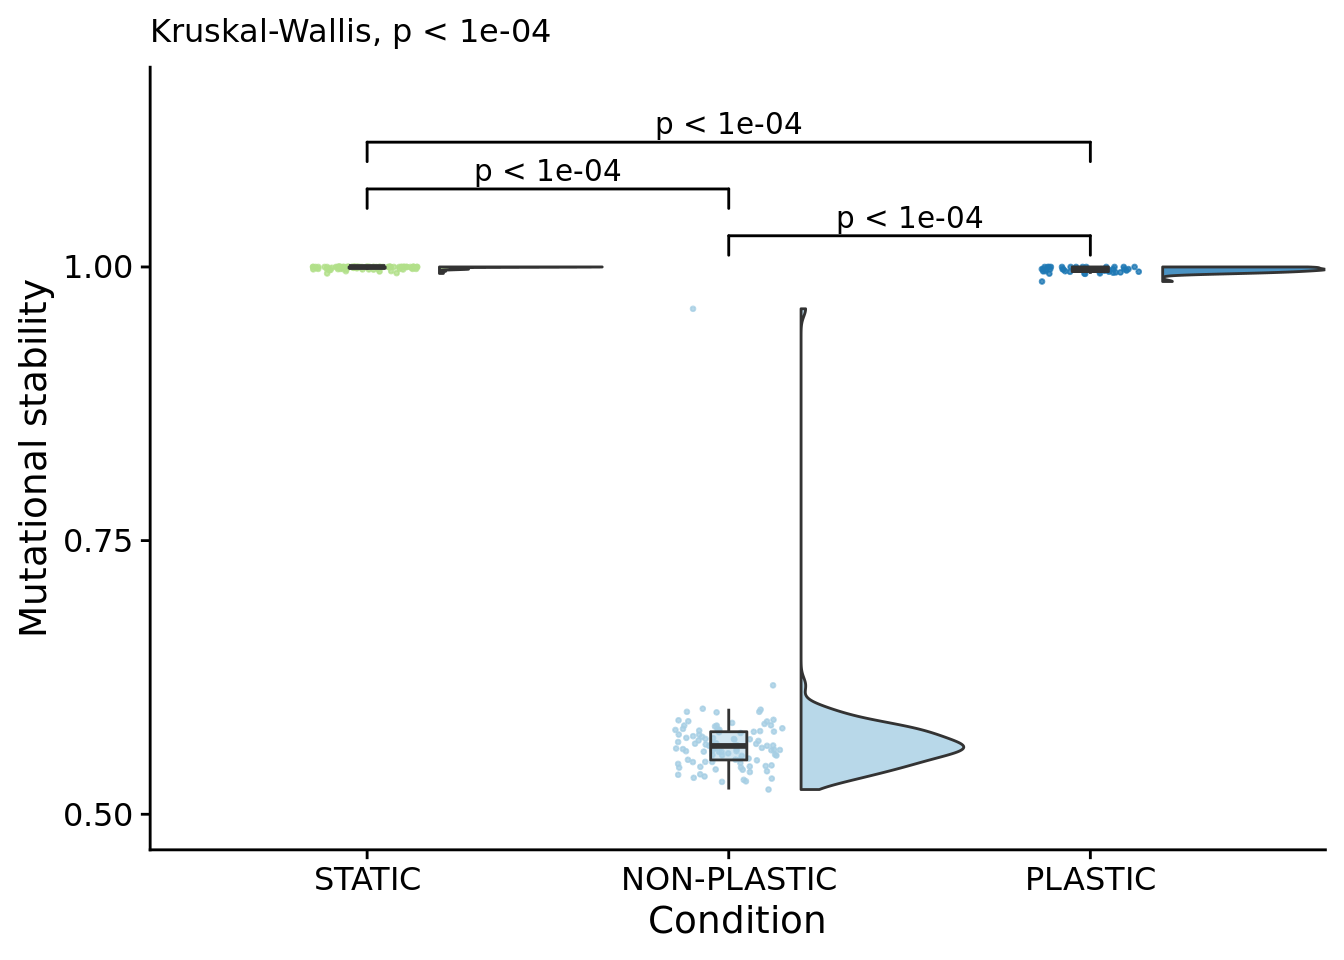
\includegraphics{supplemental-material_files/figure-latex/unnamed-chunk-34-1.pdf}

\begin{Shaded}
\begin{Highlighting}[]
\KeywordTok{kruskal.test}\NormalTok{(}
  \DataTypeTok{formula=}\NormalTok{frac_phenotype_stable_mut_steps}\OperatorTok{~}\NormalTok{condition,}
  \DataTypeTok{data=}\NormalTok{summary_data}
\NormalTok{)}
\end{Highlighting}
\end{Shaded}

\begin{verbatim}
## 
##  Kruskal-Wallis rank sum test
## 
## data:  frac_phenotype_stable_mut_steps by condition
## Kruskal-Wallis chi-squared = 191.23, df = 2, p-value < 2.2e-16
\end{verbatim}

\begin{Shaded}
\begin{Highlighting}[]
\KeywordTok{pairwise.wilcox.test}\NormalTok{(}
  \DataTypeTok{x=}\NormalTok{summary_data}\OperatorTok{$}\NormalTok{frac_phenotype_stable_mut_steps,}
  \DataTypeTok{g=}\NormalTok{summary_data}\OperatorTok{$}\NormalTok{condition,}
  \DataTypeTok{p.adjust.method=}\StringTok{"bonferroni"}\NormalTok{,}
\NormalTok{)}
\end{Highlighting}
\end{Shaded}

\begin{verbatim}
## 
##  Pairwise comparisons using Wilcoxon rank sum test with continuity correction 
## 
## data:  summary_data$frac_phenotype_stable_mut_steps and summary_data$condition 
## 
##         NON-PLASTIC PLASTIC
## PLASTIC < 2e-16     -      
## STATIC  < 2e-16     2.3e-07
## 
## P value adjustment method: bonferroni
\end{verbatim}

\begin{Shaded}
\begin{Highlighting}[]
\KeywordTok{paste}\NormalTok{(}
  \DataTypeTok{sep=}\StringTok{"; "}\NormalTok{,}
  \KeywordTok{paste0}\NormalTok{(}
    \StringTok{"PLASTIC median: "}\NormalTok{,}
    \KeywordTok{median}\NormalTok{(}\KeywordTok{filter}\NormalTok{(summary_data, condition}\OperatorTok{==}\StringTok{"PLASTIC"}\NormalTok{)}\OperatorTok{$}\NormalTok{frac_phenotype_stable_mut_steps)}
\NormalTok{  ),}
  \KeywordTok{paste0}\NormalTok{(}
    \StringTok{"STATIC median: "}\NormalTok{,}
    \KeywordTok{median}\NormalTok{(}\KeywordTok{filter}\NormalTok{(summary_data, condition}\OperatorTok{==}\StringTok{"STATIC"}\NormalTok{)}\OperatorTok{$}\NormalTok{frac_phenotype_stable_mut_steps)}
\NormalTok{  ),}
  \KeywordTok{paste0}\NormalTok{(}
    \StringTok{"NON-PLASTIC median: "}\NormalTok{,}
    \KeywordTok{median}\NormalTok{(}\KeywordTok{filter}\NormalTok{(summary_data, condition}\OperatorTok{==}\StringTok{"NON-PLASTIC"}\NormalTok{)}\OperatorTok{$}\NormalTok{frac_phenotype_stable_mut_steps)}
\NormalTok{  )}
\NormalTok{)}
\end{Highlighting}
\end{Shaded}

\begin{verbatim}
## [1] "PLASTIC median: 0.997750582573839; STATIC median: 1; NON-PLASTIC median: 0.562416981675453"
\end{verbatim}

\begin{Shaded}
\begin{Highlighting}[]
\KeywordTok{print}\NormalTok{(}\StringTok{"Wilcox rank sum test statistics:"}\NormalTok{)}
\end{Highlighting}
\end{Shaded}

\begin{verbatim}
## [1] "Wilcox rank sum test statistics:"
\end{verbatim}

\begin{Shaded}
\begin{Highlighting}[]
\ControlFlowTok{for}\NormalTok{ (pair }\ControlFlowTok{in}\NormalTok{ pairwise_comparisons) \{}
\NormalTok{  pair_data <-}\StringTok{ }\KeywordTok{filter}\NormalTok{(summary_data, condition }\OperatorTok\StringTok{ }\NormalTok{pair)}
\NormalTok{  pair_data}\OperatorTok{$}\NormalTok{condition <-}\StringTok{ }\KeywordTok{as.factor}\NormalTok{(pair_data}\OperatorTok{$}\NormalTok{condition)}
\NormalTok{  wt <-}\StringTok{ }\KeywordTok{wilcox.test}\NormalTok{(}
    \DataTypeTok{formula=}\NormalTok{frac_phenotype_stable_mut_steps}\OperatorTok{~}\NormalTok{condition,}
    \DataTypeTok{data=}\NormalTok{pair_data,}
    \DataTypeTok{exact=}\OtherTok{FALSE}\NormalTok{,}
    \DataTypeTok{paired=}\OtherTok{FALSE}
\NormalTok{  )}
  \KeywordTok{print}\NormalTok{(}\KeywordTok{paste0}\NormalTok{(pair[}\DecValTok{1}\NormalTok{], }\StringTok{"<-->"}\NormalTok{, pair[}\DecValTok{2}\NormalTok{], }\StringTok{": W="}\NormalTok{,wt}\OperatorTok{$}\NormalTok{statistic))}
\NormalTok{\}}
\end{Highlighting}
\end{Shaded}

\begin{verbatim}
## [1] "STATIC<-->NON-PLASTIC: W=0"
## [1] "STATIC<-->PLASTIC: W=1028"
## [1] "PLASTIC<-->NON-PLASTIC: W=0"
\end{verbatim}

\hypertarget{for-plastic-populations-what-fraction-of-phenotype-altering-mutations-occurred-in-the-unexpressed-phenotype}{%
\subsection{For PLASTIC populations, what fraction of phenotype-altering mutations occurred in the unexpressed phenotype?}\label{for-plastic-populations-what-fraction-of-phenotype-altering-mutations-occurred-in-the-unexpressed-phenotype}}

\begin{Shaded}
\begin{Highlighting}[]
\NormalTok{summary_data}\OperatorTok{$}\NormalTok{frac_unexpressed_mut_steps <-}\StringTok{ }\NormalTok{summary_data}\OperatorTok{$}\NormalTok{dominant_lineage_num_mut_steps_that_change_unexpressed_phenotype }\OperatorTok{/}\StringTok{ }\NormalTok{summary_data}\OperatorTok{$}\NormalTok{dominant_lineage_num_mut_steps_that_change_aggregate_phenotype}
\NormalTok{summary_data}\OperatorTok{$}\NormalTok{frac_expressed_mut_steps <-}\StringTok{ }\NormalTok{summary_data}\OperatorTok{$}\NormalTok{dominant_lineage_num_mut_steps_that_change_expressed_phenotype }\OperatorTok{/}\StringTok{ }\NormalTok{summary_data}\OperatorTok{$}\NormalTok{dominant_lineage_num_mut_steps_that_change_aggregate_phenotype}

\KeywordTok{ggplot}\NormalTok{(}\KeywordTok{filter}\NormalTok{(summary_data, condition}\OperatorTok{==}\StringTok{"PLASTIC"} \OperatorTok{&}\StringTok{ }\NormalTok{dominant_lineage_num_mut_steps_that_change_aggregate_phenotype }\OperatorTok{>}\StringTok{ }\DecValTok{0}\NormalTok{), }\KeywordTok{aes}\NormalTok{(}\DataTypeTok{x=}\NormalTok{frac_unexpressed_mut_steps)) }\OperatorTok{+}
\StringTok{  }\KeywordTok{geom_histogram}\NormalTok{(}\DataTypeTok{binwidth=}\FloatTok{0.1}\NormalTok{) }\OperatorTok{+}
\StringTok{  }\KeywordTok{scale_x_continuous}\NormalTok{(}
    \DataTypeTok{limits=}\KeywordTok{c}\NormalTok{(}\DecValTok{0}\NormalTok{, }\FloatTok{1.1}\NormalTok{),}
    \DataTypeTok{breaks=}\KeywordTok{seq}\NormalTok{(}\DecValTok{0}\NormalTok{, }\FloatTok{1.0}\NormalTok{, }\FloatTok{0.1}\NormalTok{)}
\NormalTok{  ) }\OperatorTok{+}
\StringTok{  }\KeywordTok{theme}\NormalTok{(}
    \DataTypeTok{legend.position=}\StringTok{"none"}
\NormalTok{  )}
\end{Highlighting}
\end{Shaded}

\begin{verbatim}
## Warning: Removed 2 rows containing missing values (geom_bar).
\end{verbatim}

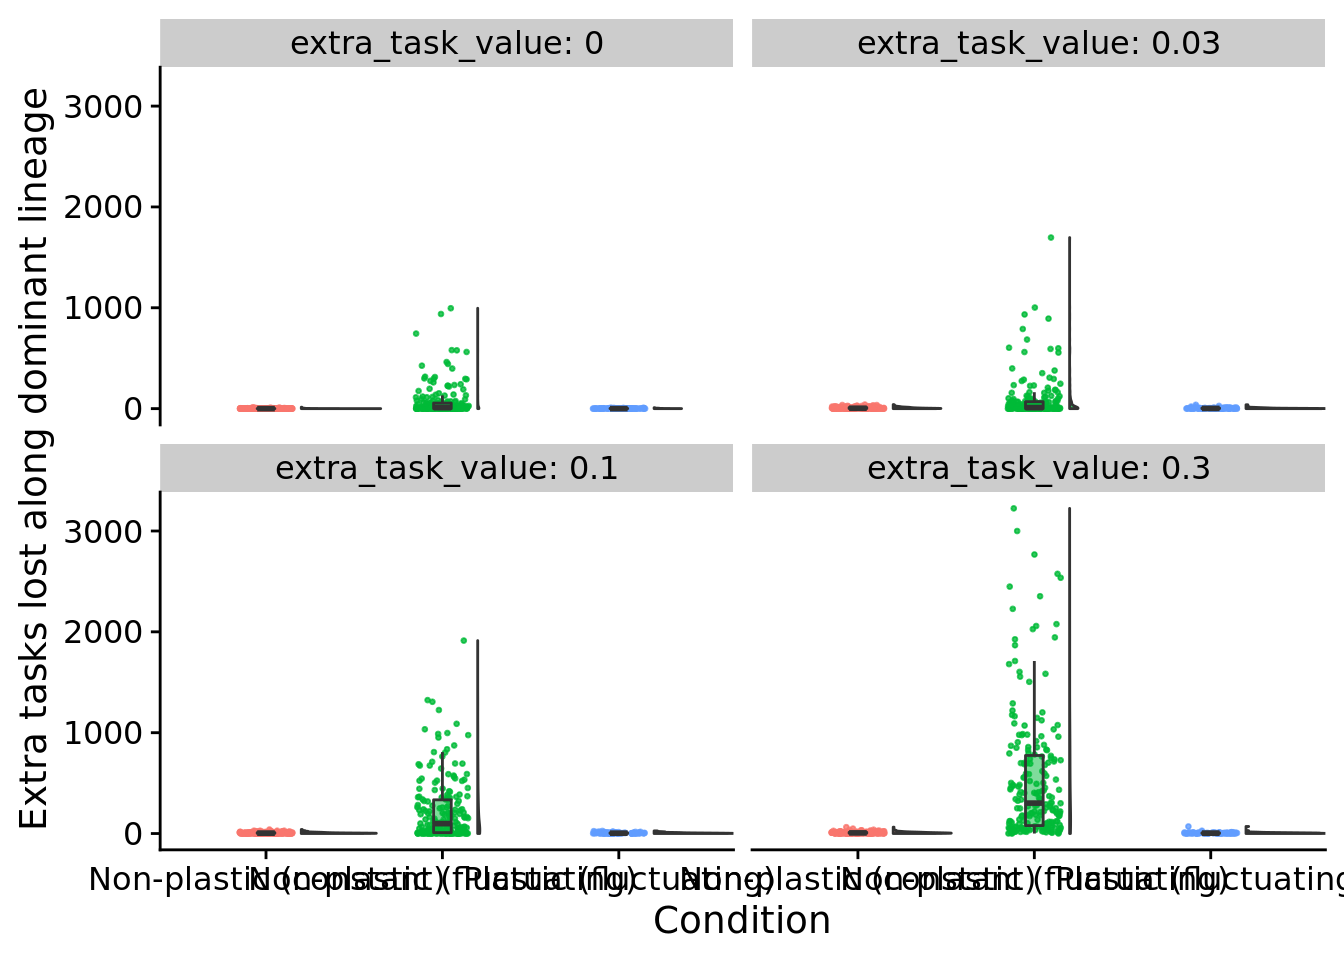
\includegraphics{supplemental-material_files/figure-latex/unnamed-chunk-36-1.pdf}

\begin{Shaded}
\begin{Highlighting}[]
\KeywordTok{print}\NormalTok{(}\KeywordTok{paste0}\NormalTok{(}\StringTok{"PLASTIC - Mean with bootstrapped 95% CI"}\NormalTok{))}
\end{Highlighting}
\end{Shaded}

\begin{verbatim}
## [1] "PLASTIC - Mean with bootstrapped 95% CI"
\end{verbatim}

\begin{Shaded}
\begin{Highlighting}[]
\NormalTok{bo <-}\StringTok{ }\KeywordTok{boot}\NormalTok{(}\KeywordTok{filter}\NormalTok{(summary_data, condition}\OperatorTok{==}\StringTok{"PLASTIC"} \OperatorTok{&}\StringTok{ }\NormalTok{dominant_lineage_num_mut_steps_that_change_aggregate_phenotype }\OperatorTok{>}\StringTok{ }\DecValTok{0}\NormalTok{)}\OperatorTok{$}\NormalTok{frac_unexpressed_mut_steps, }\DataTypeTok{statistic=}\NormalTok{samplemean, }\DataTypeTok{R=}\DecValTok{10000}\NormalTok{)}
\KeywordTok{print}\NormalTok{(bo)}
\end{Highlighting}
\end{Shaded}

\begin{verbatim}
## 
## ORDINARY NONPARAMETRIC BOOTSTRAP
## 
## 
## Call:
## boot(data = filter(summary_data, condition == "PLASTIC" & dominant_lineage_num_mut_steps_that_change_aggregate_phenotype > 
##     0)$frac_unexpressed_mut_steps, statistic = samplemean, R = 10000)
## 
## 
## Bootstrap Statistics :
##      original       bias    std. error
## t1* 0.8247126 4.511494e-05  0.03989478
\end{verbatim}

\begin{Shaded}
\begin{Highlighting}[]
\KeywordTok{print}\NormalTok{(}\KeywordTok{boot.ci}\NormalTok{(bo, }\DataTypeTok{conf=}\FloatTok{0.95}\NormalTok{, }\DataTypeTok{type=}\StringTok{"perc"}\NormalTok{))}
\end{Highlighting}
\end{Shaded}

\begin{verbatim}
## BOOTSTRAP CONFIDENCE INTERVAL CALCULATIONS
## Based on 10000 bootstrap replicates
## 
## CALL : 
## boot.ci(boot.out = bo, conf = 0.95, type = "perc")
## 
## Intervals : 
## Level     Percentile     
## 95%   ( 0.7443,  0.8994 )  
## Calculations and Intervals on Original Scale
\end{verbatim}

\begin{Shaded}
\begin{Highlighting}[]
\NormalTok{plastic_summary_data <-}\StringTok{ }\KeywordTok{filter}\NormalTok{(summary_data, condition}\OperatorTok{==}\StringTok{"PLASTIC"}\NormalTok{)}
\NormalTok{aggregate_frac_mut_steps_that_change_unexpressed_phenotype <-}\StringTok{ }\KeywordTok{sum}\NormalTok{(plastic_summary_data}\OperatorTok{$}\NormalTok{dominant_lineage_num_mut_steps_that_change_unexpressed_phenotype) }\OperatorTok{/}\StringTok{ }\KeywordTok{sum}\NormalTok{(plastic_summary_data}\OperatorTok{$}\NormalTok{dominant_lineage_num_mut_steps_that_change_aggregate_phenotype)}
\KeywordTok{sum}\NormalTok{(plastic_summary_data}\OperatorTok{$}\NormalTok{dominant_lineage_num_mut_steps_that_change_unexpressed_phenotype)}
\end{Highlighting}
\end{Shaded}

\begin{verbatim}
## [1] 83
\end{verbatim}

\begin{Shaded}
\begin{Highlighting}[]
\KeywordTok{sum}\NormalTok{(plastic_summary_data}\OperatorTok{$}\NormalTok{dominant_lineage_num_mut_steps_that_change_aggregate_phenotype)}
\end{Highlighting}
\end{Shaded}

\begin{verbatim}
## [1] 102
\end{verbatim}

\begin{Shaded}
\begin{Highlighting}[]
\NormalTok{aggregate_frac_mut_steps_that_change_unexpressed_phenotype}
\end{Highlighting}
\end{Shaded}

\begin{verbatim}
## [1] 0.8137255
\end{verbatim}

83 / 102 (0.8137255)

\hypertarget{for-plastic-populations-what-fraction-of-mutations-that-affect-the-unexpressed-phenotype-are-deleterious-versus-beneficial}{%
\subsection{For PLASTIC populations, what fraction of mutations that affect the unexpressed phenotype are deleterious versus beneficial?}\label{for-plastic-populations-what-fraction-of-mutations-that-affect-the-unexpressed-phenotype-are-deleterious-versus-beneficial}}

\begin{Shaded}
\begin{Highlighting}[]
\NormalTok{aggregate_frac_unexpressed_deleterious_mut_steps <-}\StringTok{ }\KeywordTok{sum}\NormalTok{(plastic_summary_data}\OperatorTok{$}\NormalTok{dominant_lineage_num_mut_steps_that_change_unexpressed_phenotype_deleterious) }\OperatorTok{/}\StringTok{ }\KeywordTok{sum}\NormalTok{(plastic_summary_data}\OperatorTok{$}\NormalTok{dominant_lineage_num_mut_steps_that_change_unexpressed_phenotype)}
\NormalTok{aggregate_frac_unexpressed_beneficial_mut_steps <-}\StringTok{ }\KeywordTok{sum}\NormalTok{(plastic_summary_data}\OperatorTok{$}\NormalTok{dominant_lineage_num_mut_steps_that_change_unexpressed_phenotype_beneficial) }\OperatorTok{/}\StringTok{ }\KeywordTok{sum}\NormalTok{(plastic_summary_data}\OperatorTok{$}\NormalTok{dominant_lineage_num_mut_steps_that_change_unexpressed_phenotype)}
\end{Highlighting}
\end{Shaded}

\hypertarget{deleterious-mutations}{%
\subsubsection{Deleterious mutations}\label{deleterious-mutations}}

\begin{Shaded}
\begin{Highlighting}[]
\NormalTok{summary_data}\OperatorTok{$}\NormalTok{frac_unexpressed_deleterious_mut_steps <-}\StringTok{ }\NormalTok{summary_data}\OperatorTok{$}\NormalTok{dominant_lineage_num_mut_steps_that_change_unexpressed_phenotype_deleterious }\OperatorTok{/}\StringTok{ }\NormalTok{summary_data}\OperatorTok{$}\NormalTok{dominant_lineage_num_mut_steps_that_change_unexpressed_phenotype}
\KeywordTok{ggplot}\NormalTok{(}
  \KeywordTok{filter}\NormalTok{(summary_data, condition}\OperatorTok{==}\StringTok{"PLASTIC"} \OperatorTok{&}\StringTok{ }\NormalTok{dominant_lineage_num_mut_steps_that_change_unexpressed_phenotype }\OperatorTok{>}\StringTok{ }\DecValTok{0}\NormalTok{),}
  \KeywordTok{aes}\NormalTok{(}\DataTypeTok{x=}\NormalTok{frac_unexpressed_deleterious_mut_steps)}
\NormalTok{  ) }\OperatorTok{+}
\StringTok{  }\KeywordTok{geom_density}\NormalTok{() }\OperatorTok{+}
\StringTok{  }\KeywordTok{theme}\NormalTok{(}
    \DataTypeTok{legend.position=}\StringTok{"none"}
\NormalTok{  )}
\end{Highlighting}
\end{Shaded}

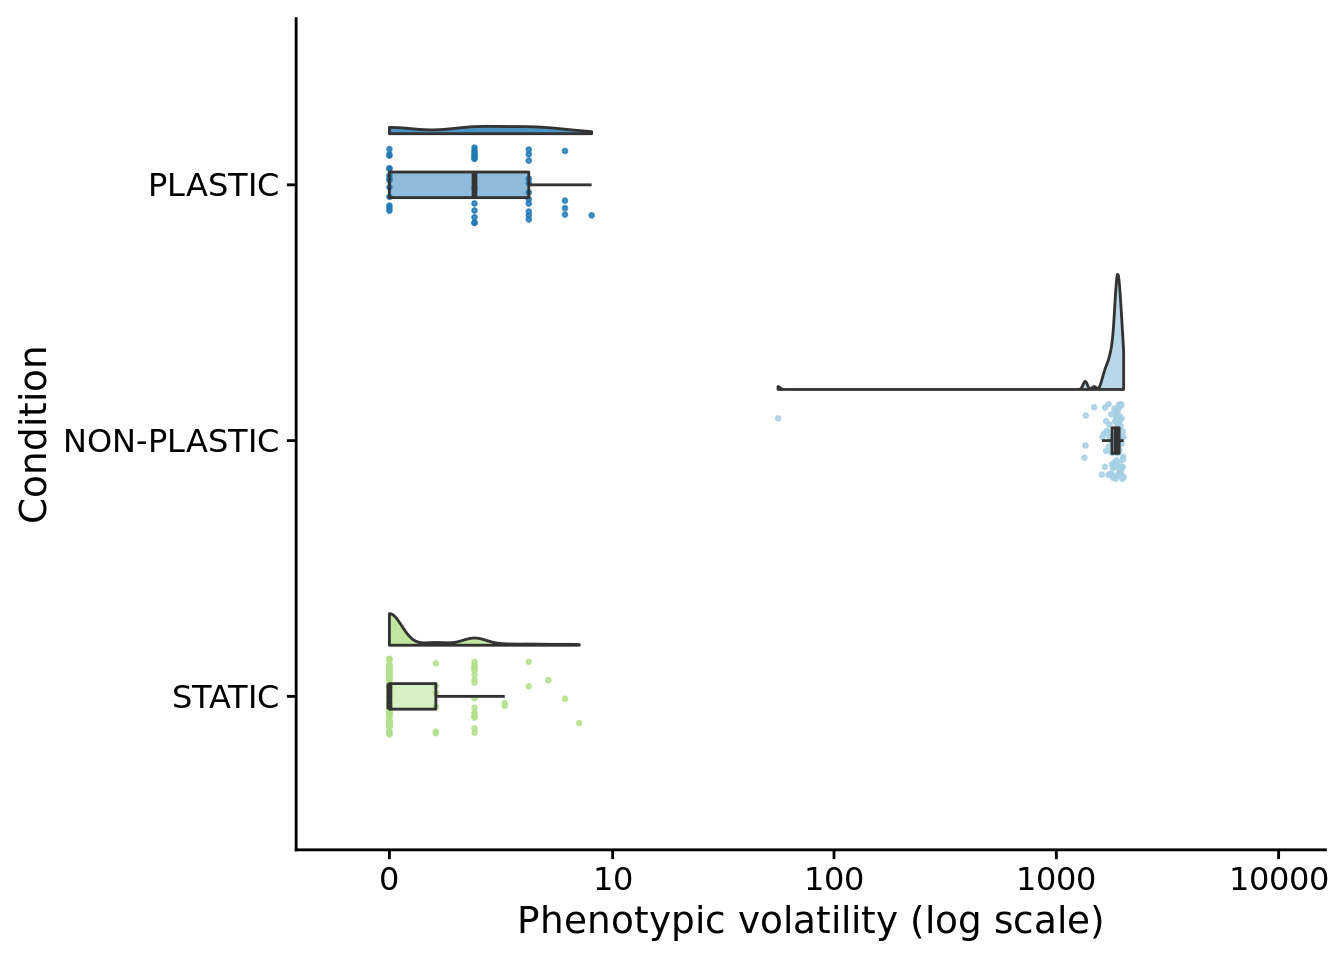
\includegraphics{supplemental-material_files/figure-latex/unnamed-chunk-39-1.pdf}

\begin{Shaded}
\begin{Highlighting}[]
\NormalTok{bo <-}\StringTok{ }\KeywordTok{boot}\NormalTok{(}\KeywordTok{filter}\NormalTok{(summary_data, condition}\OperatorTok{==}\StringTok{"PLASTIC"} \OperatorTok{&}\StringTok{ }\NormalTok{dominant_lineage_num_mut_steps_that_change_aggregate_phenotype }\OperatorTok{>}\StringTok{ }\DecValTok{0}\NormalTok{)}\OperatorTok{$}\NormalTok{frac_unexpressed_deleterious_mut_steps, }\DataTypeTok{statistic=}\NormalTok{samplemean, }\DataTypeTok{R=}\DecValTok{10000}\NormalTok{)}
\KeywordTok{print}\NormalTok{(bo)}
\end{Highlighting}
\end{Shaded}

\begin{verbatim}
## 
## ORDINARY NONPARAMETRIC BOOTSTRAP
## 
## 
## Call:
## boot(data = filter(summary_data, condition == "PLASTIC" & dominant_lineage_num_mut_steps_that_change_aggregate_phenotype > 
##     0)$frac_unexpressed_deleterious_mut_steps, statistic = samplemean, 
##     R = 10000)
## 
## 
## Bootstrap Statistics :
##      original        bias    std. error
## t1* 0.5172414 -0.0003833333  0.03956964
\end{verbatim}

\begin{Shaded}
\begin{Highlighting}[]
\KeywordTok{print}\NormalTok{(}\KeywordTok{boot.ci}\NormalTok{(bo, }\DataTypeTok{conf=}\FloatTok{0.95}\NormalTok{, }\DataTypeTok{type=}\StringTok{"perc"}\NormalTok{))}
\end{Highlighting}
\end{Shaded}

\begin{verbatim}
## BOOTSTRAP CONFIDENCE INTERVAL CALCULATIONS
## Based on 10000 bootstrap replicates
## 
## CALL : 
## boot.ci(boot.out = bo, conf = 0.95, type = "perc")
## 
## Intervals : 
## Level     Percentile     
## 95%   ( 0.4414,  0.5954 )  
## Calculations and Intervals on Original Scale
\end{verbatim}

\hypertarget{beneficial-mutations}{%
\subsubsection{Beneficial mutations}\label{beneficial-mutations}}

\begin{Shaded}
\begin{Highlighting}[]
\NormalTok{summary_data}\OperatorTok{$}\NormalTok{frac_unexpressed_beneficial_mut_steps <-}\StringTok{ }\NormalTok{summary_data}\OperatorTok{$}\NormalTok{dominant_lineage_num_mut_steps_that_change_unexpressed_phenotype_beneficial }\OperatorTok{/}\StringTok{ }\NormalTok{summary_data}\OperatorTok{$}\NormalTok{dominant_lineage_num_mut_steps_that_change_unexpressed_phenotype}

\KeywordTok{ggplot}\NormalTok{(}
  \KeywordTok{filter}\NormalTok{(summary_data, condition}\OperatorTok{==}\StringTok{"PLASTIC"} \OperatorTok{&}\StringTok{ }\NormalTok{dominant_lineage_num_mut_steps_that_change_unexpressed_phenotype }\OperatorTok{>}\StringTok{ }\DecValTok{0}\NormalTok{),}
  \KeywordTok{aes}\NormalTok{(}\DataTypeTok{x=}\NormalTok{frac_unexpressed_beneficial_mut_steps)}
\NormalTok{  ) }\OperatorTok{+}
\StringTok{  }\KeywordTok{geom_density}\NormalTok{() }\OperatorTok{+}
\StringTok{  }\KeywordTok{theme}\NormalTok{(}
    \DataTypeTok{legend.position=}\StringTok{"none"}
\NormalTok{  )}
\end{Highlighting}
\end{Shaded}

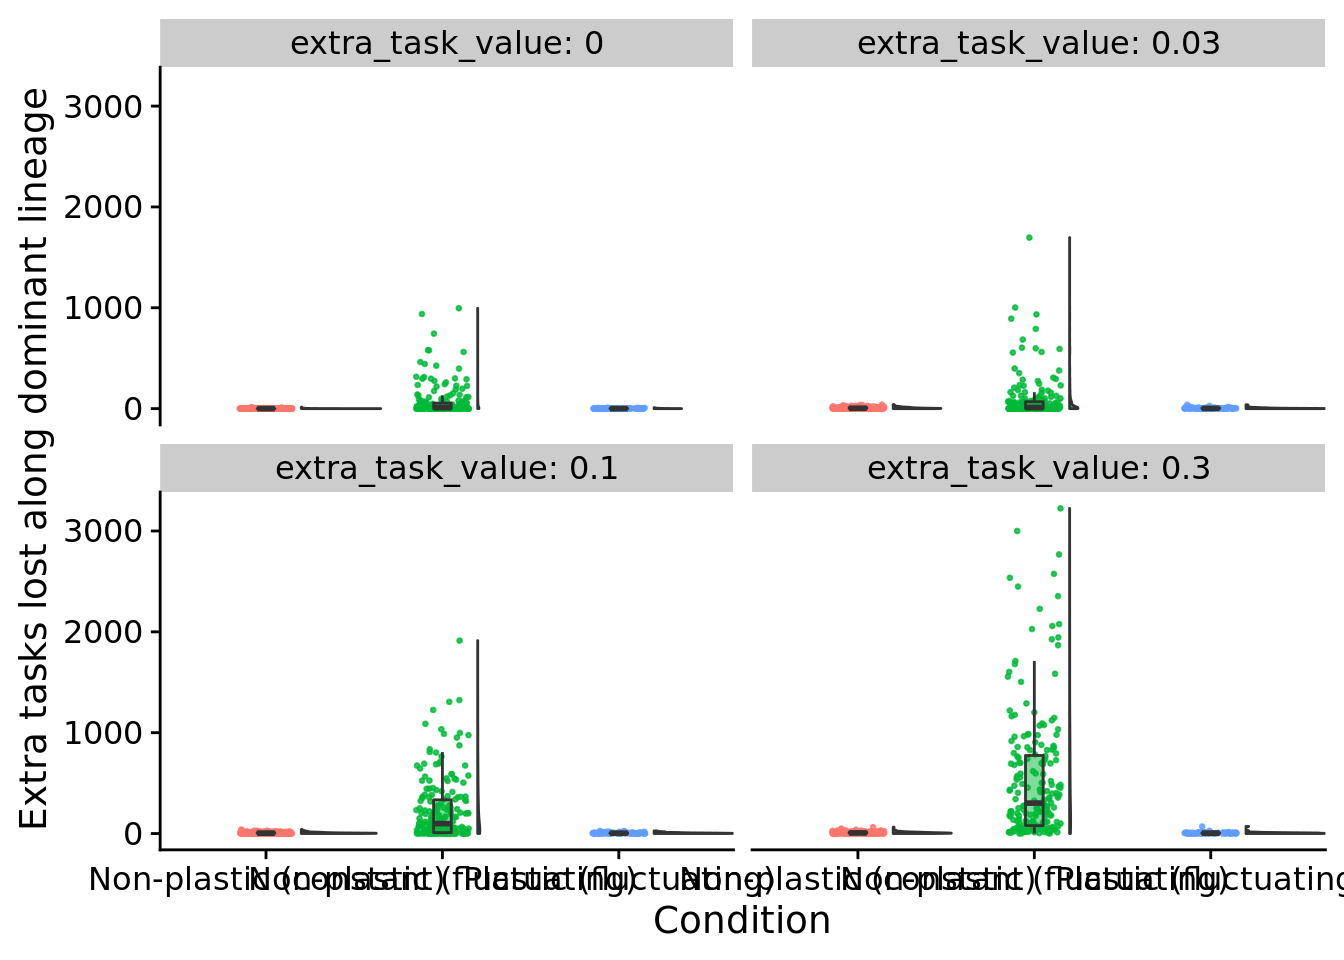
\includegraphics{supplemental-material_files/figure-latex/unnamed-chunk-40-1.pdf}

\begin{Shaded}
\begin{Highlighting}[]
\NormalTok{bo <-}\StringTok{ }\KeywordTok{boot}\NormalTok{(}\KeywordTok{filter}\NormalTok{(summary_data, condition}\OperatorTok{==}\StringTok{"PLASTIC"} \OperatorTok{&}\StringTok{ }\NormalTok{dominant_lineage_num_mut_steps_that_change_aggregate_phenotype }\OperatorTok{>}\StringTok{ }\DecValTok{0}\NormalTok{)}\OperatorTok{$}\NormalTok{frac_unexpressed_beneficial_mut_steps, }\DataTypeTok{statistic=}\NormalTok{samplemean, }\DataTypeTok{R=}\DecValTok{10000}\NormalTok{)}
\KeywordTok{print}\NormalTok{(bo)}
\end{Highlighting}
\end{Shaded}

\begin{verbatim}
## 
## ORDINARY NONPARAMETRIC BOOTSTRAP
## 
## 
## Call:
## boot(data = filter(summary_data, condition == "PLASTIC" & dominant_lineage_num_mut_steps_that_change_aggregate_phenotype > 
##     0)$frac_unexpressed_beneficial_mut_steps, statistic = samplemean, 
##     R = 10000)
## 
## 
## Bootstrap Statistics :
##      original       bias    std. error
## t1* 0.4827586 0.0001186207   0.0401311
\end{verbatim}

\begin{Shaded}
\begin{Highlighting}[]
\KeywordTok{print}\NormalTok{(}\KeywordTok{boot.ci}\NormalTok{(bo, }\DataTypeTok{conf=}\FloatTok{0.95}\NormalTok{, }\DataTypeTok{type=}\StringTok{"perc"}\NormalTok{))}
\end{Highlighting}
\end{Shaded}

\begin{verbatim}
## BOOTSTRAP CONFIDENCE INTERVAL CALCULATIONS
## Based on 10000 bootstrap replicates
## 
## CALL : 
## boot.ci(boot.out = bo, conf = 0.95, type = "perc")
## 
## Intervals : 
## Level     Percentile     
## 95%   ( 0.4023,  0.5609 )  
## Calculations and Intervals on Original Scale
\end{verbatim}

\hypertarget{mutational-robustness}{%
\section{Mutational robustness}\label{mutational-robustness}}

Mutational robustness measures the fraction of one-step mutations on a focal genotype that result in a phenotypic change.
Here, we calculate the mutational robustness of the representative genotype from each replicate (the most abundant genotype in the final population).

This data is located in a separate .tar.gz file on OSF, so we need to load it and wrangle the data.

\begin{Shaded}
\begin{Highlighting}[]
\CommentTok{# Load the data}
\NormalTok{df_mut =}\StringTok{ }\KeywordTok{read.csv}\NormalTok{(}\KeywordTok{paste0}\NormalTok{(working_directory, }\StringTok{'mutational_robustness/data/aggregated_mutant_data.csv'}\NormalTok{))}
\CommentTok{# Extract the treatment for each line}
\NormalTok{df_mut}\OperatorTok{$}\NormalTok{treatment =}\StringTok{ 'STATIC'}
\NormalTok{df_mut[df_mut}\OperatorTok{$}\NormalTok{environment }\OperatorTok{==}\StringTok{ 'chg-u100'}\NormalTok{,]}\OperatorTok{$}\NormalTok{treatment =}\StringTok{ 'PLASTIC'}
\NormalTok{df_mut[df_mut}\OperatorTok{$}\NormalTok{environment }\OperatorTok{==}\StringTok{ 'chg-u100'} \OperatorTok{&}\StringTok{ }\NormalTok{df_mut}\OperatorTok{$}\NormalTok{sensors }\OperatorTok{==}\StringTok{ }\NormalTok{F,]}\OperatorTok{$}\NormalTok{treatment =}\StringTok{ 'NON-PLASTIC'}
\NormalTok{df_mut}\OperatorTok{$}\NormalTok{treatment_factor =}\StringTok{ }\KeywordTok{factor}\NormalTok{(df_mut}\OperatorTok{$}\NormalTok{treatment, }\DataTypeTok{levels =} \KeywordTok{c}\NormalTok{(}\StringTok{'STATIC'}\NormalTok{, }\StringTok{'NON-PLASTIC'}\NormalTok{, }\StringTok{'PLASTIC'}\NormalTok{))}
\CommentTok{# For compatibility with is_outlier above}
\NormalTok{df_mut}\OperatorTok{$}\NormalTok{condition =}\StringTok{ }\NormalTok{df_mut}\OperatorTok{$}\NormalTok{treatment_factor}
\CommentTok{# Calculate robustness (originally calculated as volatility)}
\NormalTok{df_mut}\OperatorTok{$}\NormalTok{mutational_robustness =}\StringTok{ }\DecValTok{1} \OperatorTok{-}\StringTok{ }\NormalTok{df_mut}\OperatorTok{$}\NormalTok{one_step_diff_pheno_frac}
\end{Highlighting}
\end{Shaded}

Now we can plot mutational robustness:

\begin{Shaded}
\begin{Highlighting}[]
\CommentTok{# Compute manual labels for geom_signif}
\NormalTok{stat.test <-}\StringTok{ }\NormalTok{df_mut }\OperatorTok
\StringTok{  }\KeywordTok{wilcox_test}\NormalTok{(mutational_robustness }\OperatorTok{~}\StringTok{ }\NormalTok{treatment_factor) }\OperatorTok
\StringTok{  }\KeywordTok{adjust_pvalue}\NormalTok{(}\DataTypeTok{method =} \StringTok{"bonferroni"}\NormalTok{) }\OperatorTok
\StringTok{  }\KeywordTok{add_significance}\NormalTok{() }\OperatorTok
\StringTok{  }\KeywordTok{add_xy_position}\NormalTok{(}\DataTypeTok{x=}\StringTok{"treatment_factor"}\NormalTok{)}
\CommentTok{# Tweak y.position manually to account for scaled axis (edge case that triggers bad behavior in geom_signif)}
\NormalTok{stat.test}\OperatorTok{$}\NormalTok{manual_position <-}\StringTok{   }\NormalTok{stat.test}\OperatorTok{$}\NormalTok{y.position }\OperatorTok{*}\StringTok{ }\KeywordTok{c}\NormalTok{(}\FloatTok{1.05}\NormalTok{,}\FloatTok{1.1}\NormalTok{,}\FloatTok{1.15}\NormalTok{)}
\NormalTok{stat.test}\OperatorTok{$}\NormalTok{label <-}\StringTok{ }\KeywordTok{mapply}\NormalTok{(p_label,stat.test}\OperatorTok{$}\NormalTok{p.adj)}
\NormalTok{df_mut}\OperatorTok{$}\NormalTok{is_outlier <-}\StringTok{ }\KeywordTok{mapply}\NormalTok{(}
\NormalTok{  is_outlier,}
\NormalTok{  df_mut}\OperatorTok{$}\NormalTok{mutational_robustness,}
\NormalTok{  df_mut}\OperatorTok{$}\NormalTok{treatment_factor,}
  \DataTypeTok{MoreArgs=}\KeywordTok{list}\NormalTok{(}\DataTypeTok{data=}\NormalTok{df_mut, }\DataTypeTok{column=}\StringTok{"mutational_robustness"}\NormalTok{)}
\NormalTok{)}

\CommentTok{# Remap colors so that colors map}
\NormalTok{color_map =}\StringTok{ }\KeywordTok{c}\NormalTok{(}
  \StringTok{'STATIC'}\NormalTok{ =}\StringTok{ }\KeywordTok{brewer.pal}\NormalTok{(}\DecValTok{3}\NormalTok{, cb_palette)[}\DecValTok{3}\NormalTok{],}
  \StringTok{'PLASTIC'}\NormalTok{ =}\StringTok{ }\KeywordTok{brewer.pal}\NormalTok{(}\DecValTok{3}\NormalTok{, cb_palette)[}\DecValTok{2}\NormalTok{],}
  \StringTok{'NON-PLASTIC'}\NormalTok{ =}\StringTok{ }\KeywordTok{brewer.pal}\NormalTok{(}\DecValTok{3}\NormalTok{, cb_palette)[}\DecValTok{1}\NormalTok{]}
\NormalTok{)}

\CommentTok{# Plot!}
\NormalTok{mut_robustness_fig <-}\StringTok{ }\KeywordTok{ggplot}\NormalTok{(df_mut, }\KeywordTok{aes}\NormalTok{(}\DataTypeTok{x=}\NormalTok{treatment_factor, }\DataTypeTok{y=}\NormalTok{mutational_robustness, }\DataTypeTok{fill=}\NormalTok{treatment_factor)) }\OperatorTok{+}
\StringTok{  }\KeywordTok{geom_flat_violin}\NormalTok{( }\DataTypeTok{data=}\KeywordTok{filter}\NormalTok{(df_mut,is_outlier}\OperatorTok{==}\OtherTok{FALSE}\NormalTok{),}
    \DataTypeTok{scale=}\StringTok{"width"}\NormalTok{, }\DataTypeTok{position =} \KeywordTok{position_nudge}\NormalTok{(}\DataTypeTok{x =} \FloatTok{.2}\NormalTok{, }\DataTypeTok{y =} \DecValTok{0}\NormalTok{), }\DataTypeTok{alpha =} \FloatTok{.8}\NormalTok{) }\OperatorTok{+}
\StringTok{  }\KeywordTok{geom_point}\NormalTok{(}\DataTypeTok{mapping=}\KeywordTok{aes}\NormalTok{(}\DataTypeTok{color=}\NormalTok{treatment_factor), }\DataTypeTok{position =} \KeywordTok{position_jitter}\NormalTok{(}\DataTypeTok{width =} \FloatTok{.15}\NormalTok{), }\DataTypeTok{size =} \FloatTok{.5}\NormalTok{, }\DataTypeTok{alpha =} \FloatTok{0.8}\NormalTok{) }\OperatorTok{+}
\StringTok{  }\KeywordTok{geom_boxplot}\NormalTok{(}\DataTypeTok{width =} \FloatTok{.1}\NormalTok{, }\DataTypeTok{outlier.shape =} \OtherTok{NA}\NormalTok{, }\DataTypeTok{alpha =} \FloatTok{0.5}\NormalTok{) }\OperatorTok{+}
\StringTok{  }\KeywordTok{scale_x_discrete}\NormalTok{( }\DataTypeTok{name=}\StringTok{"Condition"}\NormalTok{) }\OperatorTok{+}
\StringTok{  }\KeywordTok{scale_y_continuous}\NormalTok{( }\DataTypeTok{name=}\StringTok{'Mutational robustness'}\NormalTok{, }\DataTypeTok{limits=}\KeywordTok{c}\NormalTok{(}\DecValTok{0}\NormalTok{, }\DecValTok{1}\NormalTok{)) }\OperatorTok{+}
\StringTok{  }\KeywordTok{scale_fill_manual}\NormalTok{( }\DataTypeTok{values =}\NormalTok{ color_map ) }\OperatorTok{+}
\StringTok{  }\KeywordTok{scale_color_manual}\NormalTok{( }\DataTypeTok{values =}\NormalTok{ color_map ) }\OperatorTok{+}
\StringTok{  }\KeywordTok{labs}\NormalTok{( }\DataTypeTok{subtitle=}\KeywordTok{paste0}\NormalTok{( }\StringTok{"Kruskal-Wallis, "}\NormalTok{, }\KeywordTok{p_label}\NormalTok{(}\KeywordTok{signif}\NormalTok{(}\KeywordTok{kruskal.test}\NormalTok{(}\DataTypeTok{formula=}\NormalTok{mutational_robustness}\OperatorTok{~}\NormalTok{treatment_factor, }\DataTypeTok{data=}\NormalTok{df_mut)}\OperatorTok{$}\NormalTok{p.value,}\DataTypeTok{digits=}\DecValTok{5}\NormalTok{)) ) ) }\OperatorTok{+}
\StringTok{  }\NormalTok{ggsignif}\OperatorTok{::}\KeywordTok{geom_signif}\NormalTok{( }\DataTypeTok{data=}\KeywordTok{filter}\NormalTok{(stat.test, p.adj }\OperatorTok{<=}\StringTok{ }\NormalTok{alpha),  }\KeywordTok{aes}\NormalTok{(}\DataTypeTok{xmin=}\NormalTok{group1,}\DataTypeTok{xmax=}\NormalTok{group2,}\DataTypeTok{annotations=}\NormalTok{label,}\DataTypeTok{y_position=}\NormalTok{manual_position),  }\DataTypeTok{manual=}\OtherTok{TRUE}\NormalTok{, }\DataTypeTok{inherit.aes=}\OtherTok{FALSE}\NormalTok{ ) }\OperatorTok{+}
\StringTok{  }\KeywordTok{theme}\NormalTok{( }\DataTypeTok{legend.position=}\StringTok{"none"}\NormalTok{ )}
\end{Highlighting}
\end{Shaded}

\begin{verbatim}
## Warning: Ignoring unknown aesthetics: xmin, xmax, annotations, y_position
\end{verbatim}

\begin{Shaded}
\begin{Highlighting}[]
\NormalTok{mut_robustness_fig}
\end{Highlighting}
\end{Shaded}

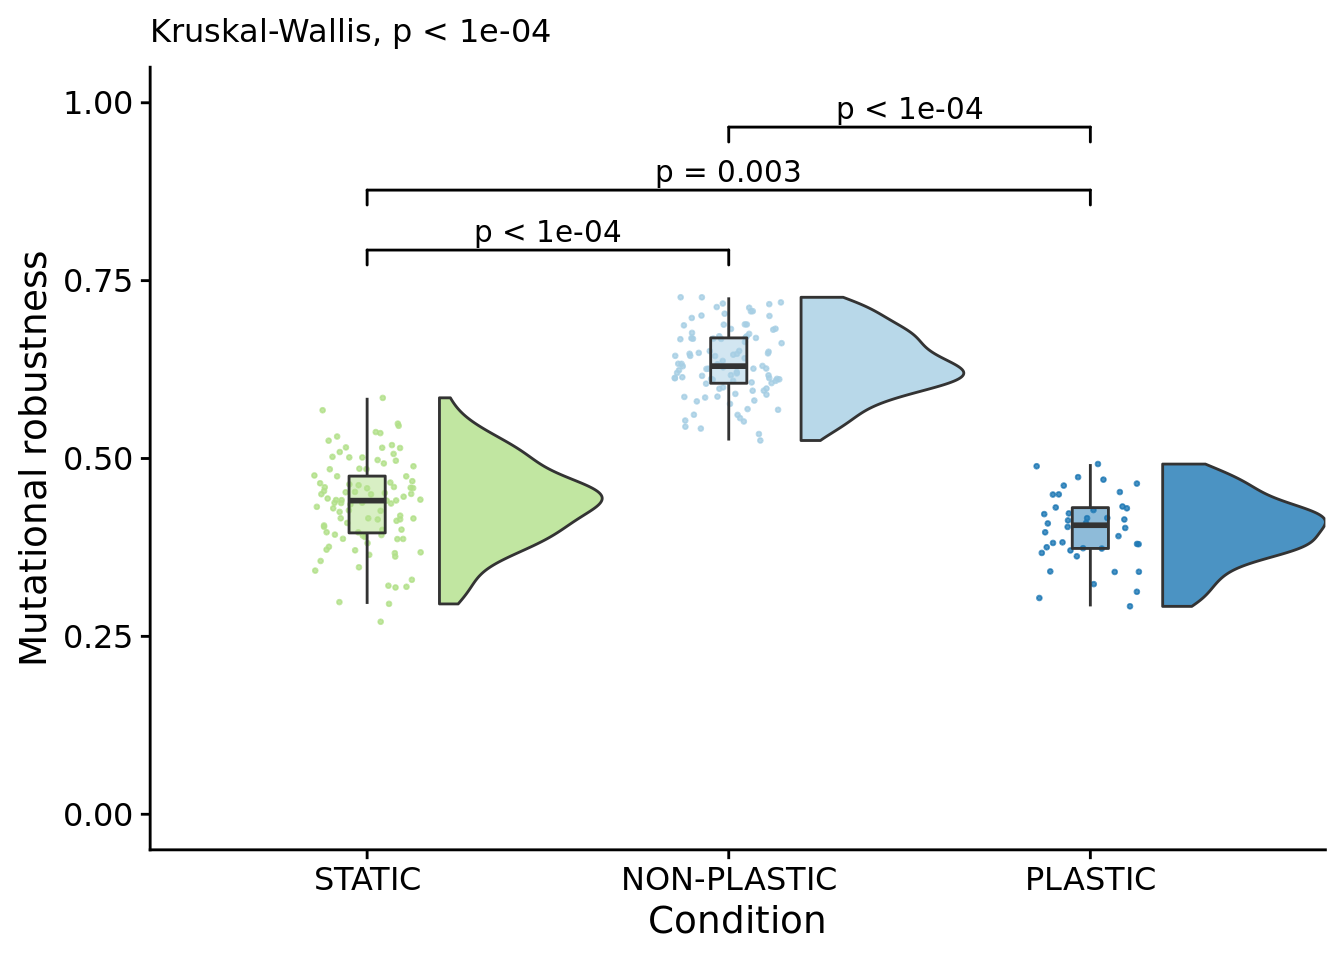
\includegraphics{supplemental-material_files/figure-latex/unnamed-chunk-42-1.pdf}

\hypertarget{manuscript-figures}{%
\section{Manuscript figures}\label{manuscript-figures}}

Figures styled for the paper.

\begin{Shaded}
\begin{Highlighting}[]
\NormalTok{magnitude_grid <-}\StringTok{ }\KeywordTok{plot_grid}\NormalTok{(}
\NormalTok{  coalescence_events_fig }\OperatorTok{+}
\StringTok{    }\KeywordTok{theme}\NormalTok{(}
      \DataTypeTok{legend.position=}\StringTok{"none"}\NormalTok{,}
      \DataTypeTok{axis.title.x=}\KeywordTok{element_blank}\NormalTok{()}
\NormalTok{    ) }\OperatorTok{+}
\StringTok{    }\KeywordTok{ggtitle}\NormalTok{(}\StringTok{"Coalescence events count"}\NormalTok{),}
\NormalTok{  mutation_count_fig }\OperatorTok{+}
\StringTok{    }\KeywordTok{theme}\NormalTok{(}
      \DataTypeTok{legend.position=}\StringTok{"none"}\NormalTok{,}
      \DataTypeTok{axis.title.x=}\KeywordTok{element_blank}\NormalTok{()}
\NormalTok{    ) }\OperatorTok{+}
\StringTok{    }\KeywordTok{ggtitle}\NormalTok{(}\StringTok{"Mutation count"}\NormalTok{),}
\NormalTok{  phenotypic_volatility_fig }\OperatorTok{+}
\StringTok{    }\KeywordTok{theme}\NormalTok{(}
      \DataTypeTok{legend.position=}\StringTok{"none"}\NormalTok{,}
      \DataTypeTok{axis.title.x=}\KeywordTok{element_blank}\NormalTok{()}
\NormalTok{    ) }\OperatorTok{+}
\StringTok{    }\KeywordTok{ggtitle}\NormalTok{(}\StringTok{"Phenotypic volatility"}\NormalTok{),}
  \DataTypeTok{nrow=}\DecValTok{1}\NormalTok{,}
  \DataTypeTok{ncol=}\DecValTok{3}\NormalTok{,}
  \DataTypeTok{align=}\StringTok{"v"}\NormalTok{,}
  \DataTypeTok{labels=}\StringTok{"auto"}
\NormalTok{)}
\NormalTok{magnitude_grid}
\end{Highlighting}
\end{Shaded}

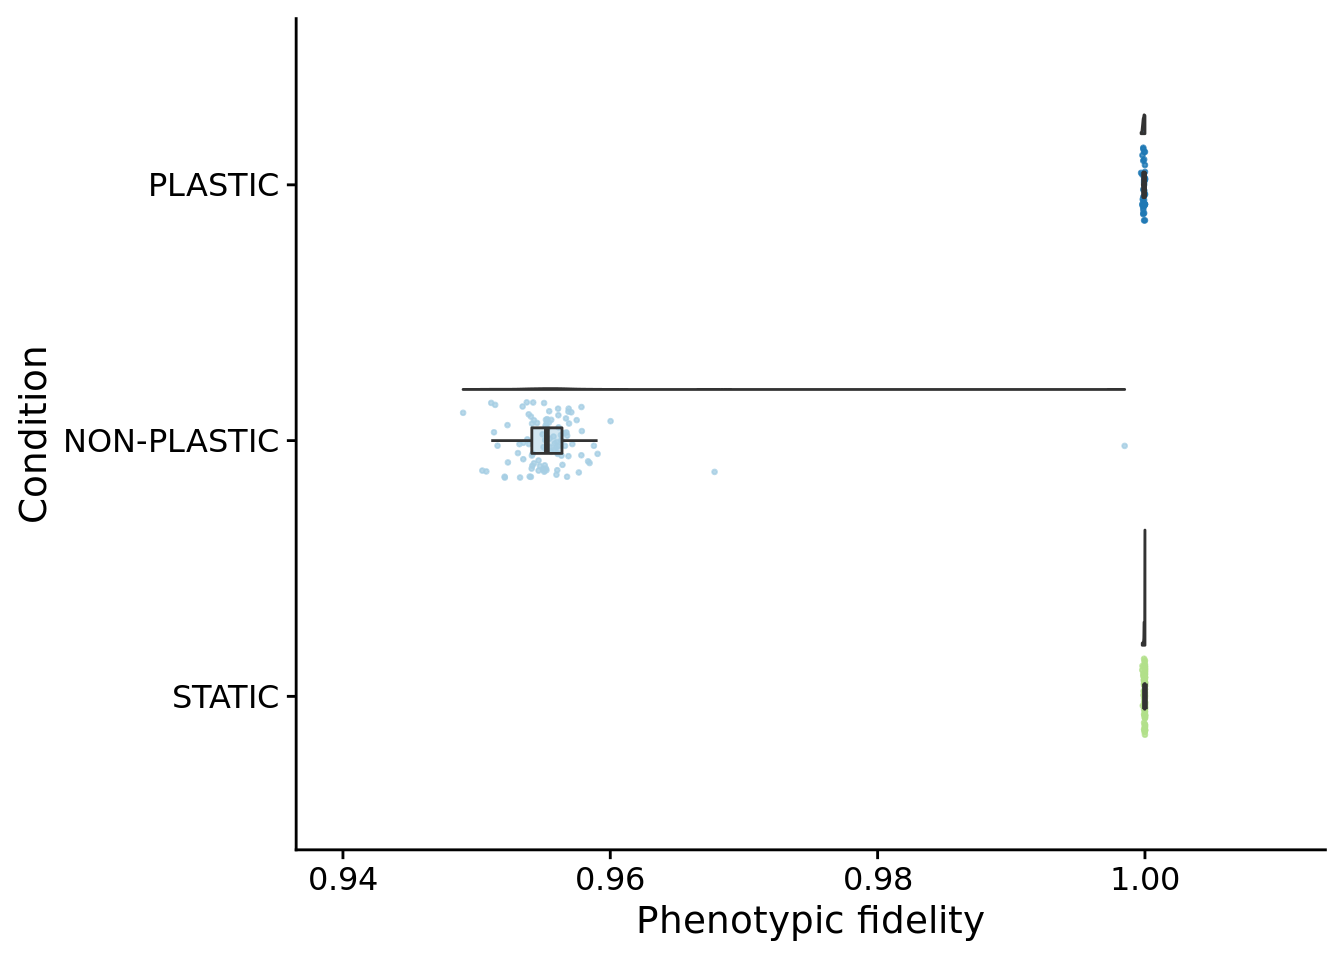
\includegraphics{supplemental-material_files/figure-latex/unnamed-chunk-43-1.pdf}

\begin{Shaded}
\begin{Highlighting}[]
\NormalTok{pace_grid <-}\StringTok{ }\KeywordTok{plot_grid}\NormalTok{(}
\NormalTok{  coalescence_events_freq_fig }\OperatorTok{+}
\StringTok{    }\KeywordTok{theme}\NormalTok{(}
      \DataTypeTok{legend.position=}\StringTok{"none"}\NormalTok{,}
      \DataTypeTok{axis.title.x=}\KeywordTok{element_blank}\NormalTok{()}
\NormalTok{    ) }\OperatorTok{+}
\StringTok{    }\KeywordTok{ggtitle}\NormalTok{(}\StringTok{"Generations between coalescence events"}\NormalTok{),}
\NormalTok{  mutational_stability_fig }\OperatorTok{+}
\StringTok{    }\KeywordTok{theme}\NormalTok{(}
      \DataTypeTok{legend.position=}\StringTok{"none"}\NormalTok{,}
      \DataTypeTok{axis.title.x=}\KeywordTok{element_blank}\NormalTok{()}
\NormalTok{    ) }\OperatorTok{+}
\StringTok{    }\KeywordTok{ggtitle}\NormalTok{(}\StringTok{"Realized mutational robustness"}\NormalTok{),}
  \DataTypeTok{nrow=}\DecValTok{1}\NormalTok{,}
  \DataTypeTok{ncol=}\DecValTok{2}\NormalTok{,}
  \DataTypeTok{align=}\StringTok{"v"}\NormalTok{,}
  \DataTypeTok{labels=}\StringTok{"auto"}
\NormalTok{)}
\NormalTok{pace_grid}
\end{Highlighting}
\end{Shaded}

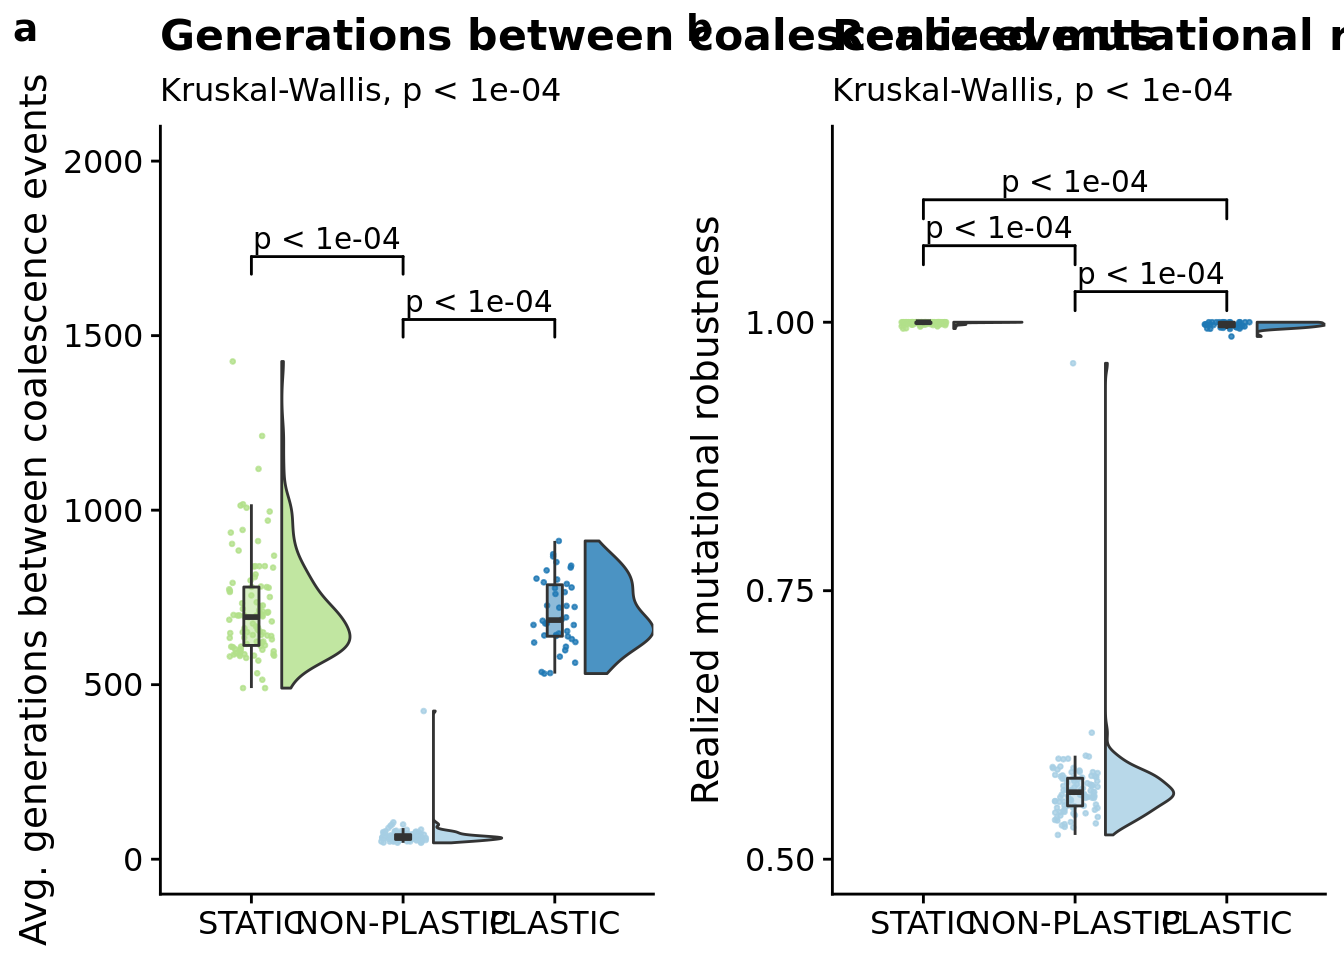
\includegraphics{supplemental-material_files/figure-latex/unnamed-chunk-43-2.pdf}

\begin{Shaded}
\begin{Highlighting}[]
\CommentTok{# Even though mutational robustness is shown by itself, this ensures it is plotted identically to the other multi-figure panels}
\NormalTok{mut_robustness_grid =}\StringTok{ }\KeywordTok{plot_grid}\NormalTok{(}
\NormalTok{  mut_robustness_fig }\OperatorTok{+}
\StringTok{    }\KeywordTok{theme}\NormalTok{(}
      \DataTypeTok{legend.position=}\StringTok{"none"}\NormalTok{,}
      \DataTypeTok{axis.title.x=}\KeywordTok{element_blank}\NormalTok{()}
\NormalTok{    ) }\OperatorTok{+}
\StringTok{    }\KeywordTok{ggtitle}\NormalTok{(}\StringTok{"Mutational robustness"}\NormalTok{),}
  \DataTypeTok{nrow=}\DecValTok{1}\NormalTok{,}
  \DataTypeTok{ncol=}\DecValTok{1}\NormalTok{,}
  \DataTypeTok{align=}\StringTok{"v"}\NormalTok{,}
  \DataTypeTok{labels=}\StringTok{""}
\NormalTok{)}
\NormalTok{mut_robustness_grid}
\end{Highlighting}
\end{Shaded}

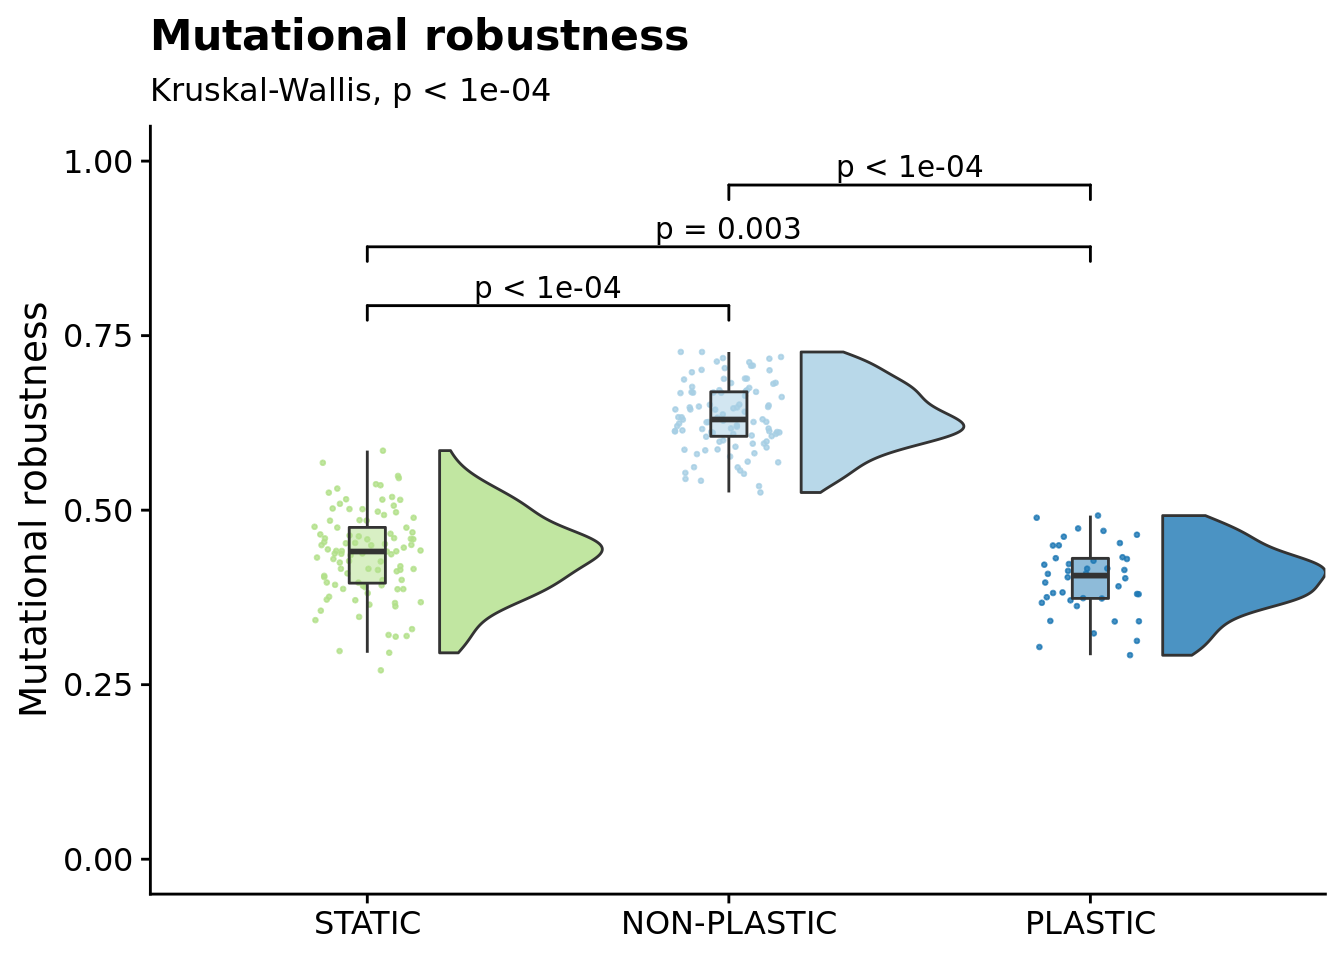
\includegraphics{supplemental-material_files/figure-latex/unnamed-chunk-43-3.pdf}

\begin{Shaded}
\begin{Highlighting}[]
\KeywordTok{save_plot}\NormalTok{(}
  \KeywordTok{paste0}\NormalTok{(working_directory, }\StringTok{"plots/"}\NormalTok{, }\StringTok{"evolutionary-change-magnitude-panel.pdf"}\NormalTok{),}
\NormalTok{  magnitude_grid,}
  \DataTypeTok{base_height=}\DecValTok{6}\NormalTok{,}
  \DataTypeTok{base_asp=}\DecValTok{3}\OperatorTok{/}\DecValTok{1}
\NormalTok{)}

\KeywordTok{save_plot}\NormalTok{(}
  \KeywordTok{paste0}\NormalTok{(working_directory, }\StringTok{"plots/"}\NormalTok{, }\StringTok{"evolutionary-change-pace-panel.pdf"}\NormalTok{),}
\NormalTok{  pace_grid,}
  \DataTypeTok{base_height=}\DecValTok{6}\NormalTok{,}
  \DataTypeTok{base_asp=}\DecValTok{2}\OperatorTok{/}\DecValTok{1}
\NormalTok{)}

\KeywordTok{save_plot}\NormalTok{(}
  \KeywordTok{paste0}\NormalTok{(working_directory, }\StringTok{"plots/"}\NormalTok{, }\StringTok{"mutational-robustness.pdf"}\NormalTok{),}
\NormalTok{  mut_robustness_grid,}
  \DataTypeTok{base_height=}\DecValTok{6}\NormalTok{,}
  \DataTypeTok{base_asp=}\DecValTok{1}
\NormalTok{)}
\end{Highlighting}
\end{Shaded}

\hypertarget{evolution-and-maintenance-of-novel-functions}{%
\chapter{Evolution and maintenance of novel functions}\label{evolution-and-maintenance-of-novel-functions}}

The effect of adaptive phenotypic plasticity on the evolution and maintenance of novel functions.

\hypertarget{overview-2}{%
\section{Overview}\label{overview-2}}

\begin{Shaded}
\begin{Highlighting}[]
\NormalTok{total_updates <-}\StringTok{ }\DecValTok{200000}
\NormalTok{replicates <-}\StringTok{ }\DecValTok{100}
\NormalTok{alpha <-}\StringTok{ }\FloatTok{0.05}

\NormalTok{focal_traits <-}\StringTok{ }\KeywordTok{c}\NormalTok{(}\StringTok{"not"}\NormalTok{,}\StringTok{"nand"}\NormalTok{,}\StringTok{"and"}\NormalTok{,}\StringTok{"ornot"}\NormalTok{,}\StringTok{"or"}\NormalTok{,}\StringTok{"andnot"}\NormalTok{)}
\NormalTok{traits_set_a <-}\StringTok{ }\KeywordTok{c}\NormalTok{(}\StringTok{"not"}\NormalTok{, }\StringTok{"and"}\NormalTok{, }\StringTok{"or"}\NormalTok{)}
\NormalTok{traits_set_b <-}\StringTok{ }\KeywordTok{c}\NormalTok{(}\StringTok{"nand"}\NormalTok{, }\StringTok{"ornot"}\NormalTok{, }\StringTok{"andnot"}\NormalTok{)}
\NormalTok{extra_traits <-}\StringTok{ }\KeywordTok{c}\NormalTok{(}
  \StringTok{"nor"}\NormalTok{,}\StringTok{"xor"}\NormalTok{,}\StringTok{"equals"}\NormalTok{,}
  \StringTok{"logic_3aa"}\NormalTok{,}\StringTok{"logic_3ab"}\NormalTok{,}\StringTok{"logic_3ac"}\NormalTok{,}
  \StringTok{"logic_3ad"}\NormalTok{,}\StringTok{"logic_3ae"}\NormalTok{,}\StringTok{"logic_3af"}\NormalTok{,}
  \StringTok{"logic_3ag"}\NormalTok{,}\StringTok{"logic_3ah"}\NormalTok{,}\StringTok{"logic_3ai"}\NormalTok{,}
  \StringTok{"logic_3aj"}\NormalTok{,}\StringTok{"logic_3ak"}\NormalTok{,}\StringTok{"logic_3al"}\NormalTok{,}
  \StringTok{"logic_3am"}\NormalTok{,}\StringTok{"logic_3an"}\NormalTok{,}\StringTok{"logic_3ao"}\NormalTok{,}
  \StringTok{"logic_3ap"}\NormalTok{,}\StringTok{"logic_3aq"}\NormalTok{,}\StringTok{"logic_3ar"}\NormalTok{,}
  \StringTok{"logic_3as"}\NormalTok{,}\StringTok{"logic_3at"}\NormalTok{,}\StringTok{"logic_3au"}\NormalTok{,}
  \StringTok{"logic_3av"}\NormalTok{,}\StringTok{"logic_3aw"}\NormalTok{,}\StringTok{"logic_3ax"}\NormalTok{,}
  \StringTok{"logic_3ay"}\NormalTok{,}\StringTok{"logic_3az"}\NormalTok{,}\StringTok{"logic_3ba"}\NormalTok{,}
  \StringTok{"logic_3bb"}\NormalTok{,}\StringTok{"logic_3bc"}\NormalTok{,}\StringTok{"logic_3bd"}\NormalTok{,}
  \StringTok{"logic_3be"}\NormalTok{,}\StringTok{"logic_3bf"}\NormalTok{,}\StringTok{"logic_3bg"}\NormalTok{,}
  \StringTok{"logic_3bh"}\NormalTok{,}\StringTok{"logic_3bi"}\NormalTok{,}\StringTok{"logic_3bj"}\NormalTok{,}
  \StringTok{"logic_3bk"}\NormalTok{,}\StringTok{"logic_3bl"}\NormalTok{,}\StringTok{"logic_3bm"}\NormalTok{,}
  \StringTok{"logic_3bn"}\NormalTok{,}\StringTok{"logic_3bo"}\NormalTok{,}\StringTok{"logic_3bp"}\NormalTok{,}
  \StringTok{"logic_3bq"}\NormalTok{,}\StringTok{"logic_3br"}\NormalTok{,}\StringTok{"logic_3bs"}\NormalTok{,}
  \StringTok{"logic_3bt"}\NormalTok{,}\StringTok{"logic_3bu"}\NormalTok{,}\StringTok{"logic_3bv"}\NormalTok{,}
  \StringTok{"logic_3bw"}\NormalTok{,}\StringTok{"logic_3bx"}\NormalTok{,}\StringTok{"logic_3by"}\NormalTok{,}
  \StringTok{"logic_3bz"}\NormalTok{,}\StringTok{"logic_3ca"}\NormalTok{,}\StringTok{"logic_3cb"}\NormalTok{,}
  \StringTok{"logic_3cc"}\NormalTok{,}\StringTok{"logic_3cd"}\NormalTok{,}\StringTok{"logic_3ce"}\NormalTok{,}
  \StringTok{"logic_3cf"}\NormalTok{,}\StringTok{"logic_3cg"}\NormalTok{,}\StringTok{"logic_3ch"}\NormalTok{,}
  \StringTok{"logic_3ci"}\NormalTok{,}\StringTok{"logic_3cj"}\NormalTok{,}\StringTok{"logic_3ck"}\NormalTok{,}
  \StringTok{"logic_3cl"}\NormalTok{,}\StringTok{"logic_3cm"}\NormalTok{,}\StringTok{"logic_3cn"}\NormalTok{,}
  \StringTok{"logic_3co"}\NormalTok{,}\StringTok{"logic_3cp"}
\NormalTok{)}

\CommentTok{# Relative location of data.}
\NormalTok{working_directory <-}\StringTok{ "experiments/2021-01-31-complex-features/analysis/"} \CommentTok{# << For bookdown}
\CommentTok{# working_directory <- "./"}
\end{Highlighting}
\end{Shaded}

\hypertarget{analysis-dependencies-2}{%
\section{Analysis dependencies}\label{analysis-dependencies-2}}

Load all required R libraries.

\begin{Shaded}
\begin{Highlighting}[]
\KeywordTok{library}\NormalTok{(ggplot2)}
\KeywordTok{library}\NormalTok{(rstatix)}
\KeywordTok{library}\NormalTok{(ggsignif)}
\KeywordTok{library}\NormalTok{(scales)}
\KeywordTok{library}\NormalTok{(tidyverse)}
\KeywordTok{library}\NormalTok{(cowplot)}
\KeywordTok{library}\NormalTok{(RColorBrewer)}
\KeywordTok{library}\NormalTok{(Hmisc)}
\KeywordTok{library}\NormalTok{(boot)}
\KeywordTok{source}\NormalTok{(}\StringTok{"https://gist.githubusercontent.com/benmarwick/2a1bb0133ff568cbe28d/raw/fb53bd97121f7f9ce947837ef1a4c65a73bffb3f/geom_flat_violin.R"}\NormalTok{)}
\end{Highlighting}
\end{Shaded}

These analyses were conducted/knitted with the following computing environment:

\begin{Shaded}
\begin{Highlighting}[]
\KeywordTok{print}\NormalTok{(version)}
\end{Highlighting}
\end{Shaded}

\begin{verbatim}
##                _                           
## platform       x86_64-pc-linux-gnu         
## arch           x86_64                      
## os             linux-gnu                   
## system         x86_64, linux-gnu           
## status                                     
## major          4                           
## minor          1.3                         
## year           2022                        
## month          03                          
## day            10                          
## svn rev        81868                       
## language       R                           
## version.string R version 4.1.3 (2022-03-10)
## nickname       One Push-Up
\end{verbatim}

\hypertarget{setup-2}{%
\section{Setup}\label{setup-2}}

\begin{Shaded}
\begin{Highlighting}[]
\CommentTok{####### summary data #######}
\NormalTok{summary_data_loc <-}\StringTok{ }\KeywordTok{paste0}\NormalTok{(working_directory, }\StringTok{"data/aggregate.csv"}\NormalTok{)}
\NormalTok{summary_data <-}\StringTok{ }\KeywordTok{read.csv}\NormalTok{(summary_data_loc, }\DataTypeTok{na.strings=}\StringTok{"NONE"}\NormalTok{)}

\NormalTok{summary_data}\OperatorTok{$}\NormalTok{DISABLE_REACTION_SENSORS <-}\StringTok{ }\KeywordTok{as.factor}\NormalTok{(summary_data}\OperatorTok{$}\NormalTok{DISABLE_REACTION_SENSORS)}
\NormalTok{summary_data}\OperatorTok{$}\NormalTok{chg_env <-}\StringTok{ }\NormalTok{summary_data}\OperatorTok{$}\NormalTok{chg_env }\OperatorTok{==}\StringTok{ "True"}
\NormalTok{summary_data}\OperatorTok{$}\NormalTok{dominant_plastic_odd_even <-}\StringTok{ }\KeywordTok{as.factor}\NormalTok{(summary_data}\OperatorTok{$}\NormalTok{dominant_plastic_odd_even)}
\NormalTok{summary_data}\OperatorTok{$}\NormalTok{sensors <-}\StringTok{ }\NormalTok{summary_data}\OperatorTok{$}\NormalTok{DISABLE_REACTION_SENSORS }\OperatorTok{==}\StringTok{ "0"}
\NormalTok{summary_data}\OperatorTok{$}\NormalTok{is_plastic <-}\StringTok{ }\NormalTok{summary_data}\OperatorTok{$}\NormalTok{dominant_plastic_odd_even }\OperatorTok{==}\StringTok{ "True"}
\NormalTok{summary_data}\OperatorTok{$}\NormalTok{extra_task_value <-}\StringTok{ }\KeywordTok{as.factor}\NormalTok{(summary_data}\OperatorTok{$}\NormalTok{extra_task_value)}
\NormalTok{summary_data <-}\StringTok{ }\KeywordTok{filter}\NormalTok{(summary_data, extra_task_value }\OperatorTok{==}\StringTok{ }\FloatTok{0.1}\NormalTok{)}

\NormalTok{env_label_fun <-}\StringTok{ }\ControlFlowTok{function}\NormalTok{(chg_env) \{}
  \ControlFlowTok{if}\NormalTok{ (chg_env) \{}
    \KeywordTok{return}\NormalTok{(}\StringTok{"Fluctuating"}\NormalTok{)}
\NormalTok{  \} }\ControlFlowTok{else}\NormalTok{ \{}
    \KeywordTok{return}\NormalTok{(}\StringTok{"Constant"}\NormalTok{)}
\NormalTok{  \}}
\NormalTok{\}}

\NormalTok{sensors_label_fun <-}\StringTok{ }\ControlFlowTok{function}\NormalTok{(has_sensors) \{}
  \ControlFlowTok{if}\NormalTok{ (has_sensors) \{}
    \KeywordTok{return}\NormalTok{(}\StringTok{"Sensors"}\NormalTok{)}
\NormalTok{  \} }\ControlFlowTok{else}\NormalTok{ \{}
    \KeywordTok{return}\NormalTok{(}\StringTok{"No sensors"}\NormalTok{)}
\NormalTok{  \}}
\NormalTok{\}}

\NormalTok{condition_label_fun <-}\StringTok{ }\ControlFlowTok{function}\NormalTok{(has_sensors, env_chg) \{}
  \ControlFlowTok{if}\NormalTok{ (has_sensors }\OperatorTok{&&}\StringTok{ }\NormalTok{env_chg) \{}
    \KeywordTok{return}\NormalTok{(}\StringTok{"PLASTIC"}\NormalTok{)}
\NormalTok{  \} }\ControlFlowTok{else} \ControlFlowTok{if}\NormalTok{ (env_chg) \{}
    \KeywordTok{return}\NormalTok{(}\StringTok{"NON-PLASTIC"}\NormalTok{)}
\NormalTok{  \} }\ControlFlowTok{else}\NormalTok{ \{}
    \KeywordTok{return}\NormalTok{(}\StringTok{"STATIC"}\NormalTok{)}
\NormalTok{  \}}
\NormalTok{\}}

\NormalTok{summary_data}\OperatorTok{$}\NormalTok{env_label <-}\StringTok{ }\KeywordTok{mapply}\NormalTok{(}
\NormalTok{  env_label_fun,}
\NormalTok{  summary_data}\OperatorTok{$}\NormalTok{chg_env}
\NormalTok{)}
\NormalTok{summary_data}\OperatorTok{$}\NormalTok{sensors_label <-}\StringTok{ }\KeywordTok{mapply}\NormalTok{(}
\NormalTok{  sensors_label_fun,}
\NormalTok{  summary_data}\OperatorTok{$}\NormalTok{sensors}
\NormalTok{)}
\NormalTok{summary_data}\OperatorTok{$}\NormalTok{condition <-}\StringTok{ }\KeywordTok{mapply}\NormalTok{(}
\NormalTok{  condition_label_fun,}
\NormalTok{  summary_data}\OperatorTok{$}\NormalTok{sensors,}
\NormalTok{  summary_data}\OperatorTok{$}\NormalTok{chg_env}
\NormalTok{)}

\NormalTok{condition_order =}\StringTok{ }\KeywordTok{c}\NormalTok{(}
  \StringTok{"STATIC"}\NormalTok{,}
  \StringTok{"NON-PLASTIC"}\NormalTok{,}
  \StringTok{"PLASTIC"}
\NormalTok{)}
\NormalTok{pairwise_comparisons <-}\StringTok{ }\KeywordTok{list}\NormalTok{(}
  \KeywordTok{c}\NormalTok{(}\StringTok{"STATIC"}\NormalTok{, }\StringTok{"NON-PLASTIC"}\NormalTok{),}
  \KeywordTok{c}\NormalTok{(}\StringTok{"STATIC"}\NormalTok{, }\StringTok{"PLASTIC"}\NormalTok{),}
  \KeywordTok{c}\NormalTok{(}\StringTok{"PLASTIC"}\NormalTok{, }\StringTok{"NON-PLASTIC"}\NormalTok{)}
\NormalTok{)}

\NormalTok{p_label <-}\StringTok{ }\ControlFlowTok{function}\NormalTok{(p_value) \{}
\NormalTok{  threshold =}\StringTok{ }\FloatTok{0.0001}
  \ControlFlowTok{if}\NormalTok{ (p_value }\OperatorTok{<}\StringTok{ }\NormalTok{threshold) \{}
    \KeywordTok{return}\NormalTok{(}\KeywordTok{paste0}\NormalTok{(}\StringTok{"p < "}\NormalTok{, threshold))}
\NormalTok{  \} }\ControlFlowTok{else}\NormalTok{ \{}
    \KeywordTok{return}\NormalTok{(}\KeywordTok{paste0}\NormalTok{(}\StringTok{"p = "}\NormalTok{, p_value))}
\NormalTok{  \}}
\NormalTok{\}}

\CommentTok{# *really* inefficient way to identify outliers}
\NormalTok{is_outlier <-}\StringTok{ }\ControlFlowTok{function}\NormalTok{(value, cond, data, column) \{}
\NormalTok{  cond_data <-}\StringTok{ }\KeywordTok{filter}\NormalTok{(data, condition}\OperatorTok{==}\NormalTok{cond)}
\NormalTok{  q1 <-}\StringTok{ }\KeywordTok{summary}\NormalTok{(cond_data[,column])[[}\StringTok{"1st Qu."}\NormalTok{]]}
\NormalTok{  q3 <-}\StringTok{ }\KeywordTok{summary}\NormalTok{(cond_data[,column])[[}\StringTok{"3rd Qu."}\NormalTok{]]}
\NormalTok{  H <-}\StringTok{ }\FloatTok{1.5} \OperatorTok{*}\StringTok{ }\KeywordTok{IQR}\NormalTok{(cond_data[,column])}
  \KeywordTok{return}\NormalTok{( (value }\OperatorTok{<}\StringTok{ }\NormalTok{(q1}\OperatorTok{-}\NormalTok{H)) }\OperatorTok{||}\StringTok{ }\NormalTok{(value }\OperatorTok{>}\StringTok{ }\NormalTok{(q3}\OperatorTok{+}\NormalTok{H)) )}
\NormalTok{\}}

\CommentTok{###### time series #####}
\NormalTok{lineage_time_series_data_loc <-}\StringTok{ }\KeywordTok{paste0}\NormalTok{(working_directory, }\StringTok{"data/lineage_series.csv"}\NormalTok{)}
\NormalTok{lineage_time_series_data <-}\StringTok{ }\KeywordTok{read.csv}\NormalTok{(lineage_time_series_data_loc)}

\NormalTok{lineage_time_series_data}\OperatorTok{$}\NormalTok{DISABLE_REACTION_SENSORS <-}\StringTok{ }\KeywordTok{as.factor}\NormalTok{(lineage_time_series_data}\OperatorTok{$}\NormalTok{DISABLE_REACTION_SENSORS)}
\NormalTok{lineage_time_series_data}\OperatorTok{$}\NormalTok{chg_env <-}\StringTok{ }\NormalTok{lineage_time_series_data}\OperatorTok{$}\NormalTok{chg_env }\OperatorTok{==}\StringTok{ "True"}
\NormalTok{lineage_time_series_data}\OperatorTok{$}\NormalTok{sensors <-}\StringTok{ }\NormalTok{lineage_time_series_data}\OperatorTok{$}\NormalTok{DISABLE_REACTION_SENSORS }\OperatorTok{==}\StringTok{ "0"}
\NormalTok{lineage_time_series_data}\OperatorTok{$}\NormalTok{extra_task_value <-}\StringTok{ }\KeywordTok{as.factor}\NormalTok{(lineage_time_series_data}\OperatorTok{$}\NormalTok{extra_task_value)}

\NormalTok{lineage_time_series_data}\OperatorTok{$}\NormalTok{env_label <-}\StringTok{ }\KeywordTok{mapply}\NormalTok{(}
\NormalTok{  env_label_fun,}
\NormalTok{  lineage_time_series_data}\OperatorTok{$}\NormalTok{chg_env}
\NormalTok{)}
\NormalTok{lineage_time_series_data}\OperatorTok{$}\NormalTok{sensors_label <-}\StringTok{ }\KeywordTok{mapply}\NormalTok{(}
\NormalTok{  sensors_label_fun,}
\NormalTok{  lineage_time_series_data}\OperatorTok{$}\NormalTok{sensors}
\NormalTok{)}
\NormalTok{lineage_time_series_data}\OperatorTok{$}\NormalTok{condition <-}\StringTok{ }\KeywordTok{mapply}\NormalTok{(}
\NormalTok{  condition_label_fun,}
\NormalTok{  lineage_time_series_data}\OperatorTok{$}\NormalTok{sensors,}
\NormalTok{  lineage_time_series_data}\OperatorTok{$}\NormalTok{chg_env}
\NormalTok{)}

\CommentTok{####### misc #######}
\CommentTok{# Configure our default graphing theme}
\KeywordTok{theme_set}\NormalTok{(}\KeywordTok{theme_cowplot}\NormalTok{())}
\CommentTok{# Palette}
\NormalTok{cb_palette <-}\StringTok{ "Paired"}
\CommentTok{# Create directory to dump plots}
\KeywordTok{dir.create}\NormalTok{(}\KeywordTok{paste0}\NormalTok{(working_directory, }\StringTok{"plots"}\NormalTok{), }\DataTypeTok{showWarnings=}\OtherTok{FALSE}\NormalTok{)}
\CommentTok{# Sample mean function}
\NormalTok{samplemean <-}\StringTok{ }\ControlFlowTok{function}\NormalTok{(x, d) \{}
  \KeywordTok{return}\NormalTok{(}\KeywordTok{mean}\NormalTok{(x[d]))}
\NormalTok{\}}
\end{Highlighting}
\end{Shaded}

\hypertarget{the-evolution-of-phenotypic-plasticity-1}{%
\section{The evolution of phenotypic plasticity}\label{the-evolution-of-phenotypic-plasticity-1}}

For sensor-enabled populations in fluctuating environments, we only transfered populations containing an optimally plastic genotype to phase two.

\begin{Shaded}
\begin{Highlighting}[]
\NormalTok{summary_data_grouped =}\StringTok{ }\NormalTok{dplyr}\OperatorTok{::}\KeywordTok{group_by}\NormalTok{(summary_data, sensors, env_label, condition, extra_task_value)}
\NormalTok{summary_data_group_counts =}\StringTok{ }\NormalTok{dplyr}\OperatorTok{::}\KeywordTok{summarize}\NormalTok{(summary_data_grouped, }\DataTypeTok{n=}\NormalTok{dplyr}\OperatorTok{::}\KeywordTok{n}\NormalTok{())}

\KeywordTok{ggplot}\NormalTok{(summary_data_group_counts, }\KeywordTok{aes}\NormalTok{(}\DataTypeTok{x=}\NormalTok{condition, }\DataTypeTok{y=}\NormalTok{n, }\DataTypeTok{fill=}\NormalTok{condition)) }\OperatorTok{+}
\StringTok{  }\KeywordTok{geom_col}\NormalTok{(}\DataTypeTok{position=}\KeywordTok{position_dodge}\NormalTok{(}\FloatTok{0.9}\NormalTok{)) }\OperatorTok{+}
\StringTok{  }\KeywordTok{geom_text}\NormalTok{(}\KeywordTok{aes}\NormalTok{(}\DataTypeTok{label=}\NormalTok{n, }\DataTypeTok{y=}\NormalTok{n}\OperatorTok{+}\DecValTok{2}\NormalTok{)) }\OperatorTok{+}
\StringTok{  }\KeywordTok{scale_x_discrete}\NormalTok{(}
    \DataTypeTok{name=}\StringTok{"Condition"}\NormalTok{,}
    \DataTypeTok{limits=}\NormalTok{condition_order}
\NormalTok{  ) }\OperatorTok{+}
\StringTok{  }\KeywordTok{scale_fill_brewer}\NormalTok{(}
    \DataTypeTok{palette=}\NormalTok{cb_palette}
\NormalTok{  ) }\OperatorTok{+}
\StringTok{  }\KeywordTok{scale_color_brewer}\NormalTok{(}
    \DataTypeTok{palette=}\NormalTok{cb_palette}
\NormalTok{  ) }\OperatorTok{+}
\StringTok{  }\KeywordTok{ylab}\NormalTok{(}\StringTok{"Number of replicates in phase two"}\NormalTok{) }\OperatorTok{+}
\StringTok{  }\KeywordTok{facet_wrap}\NormalTok{(}\OperatorTok{~}\NormalTok{extra_task_value, }\DataTypeTok{labeller=}\NormalTok{label_both) }\OperatorTok{+}
\StringTok{  }\KeywordTok{theme}\NormalTok{(}
    \DataTypeTok{legend.position=}\StringTok{"none"}
\NormalTok{  )}
\end{Highlighting}
\end{Shaded}

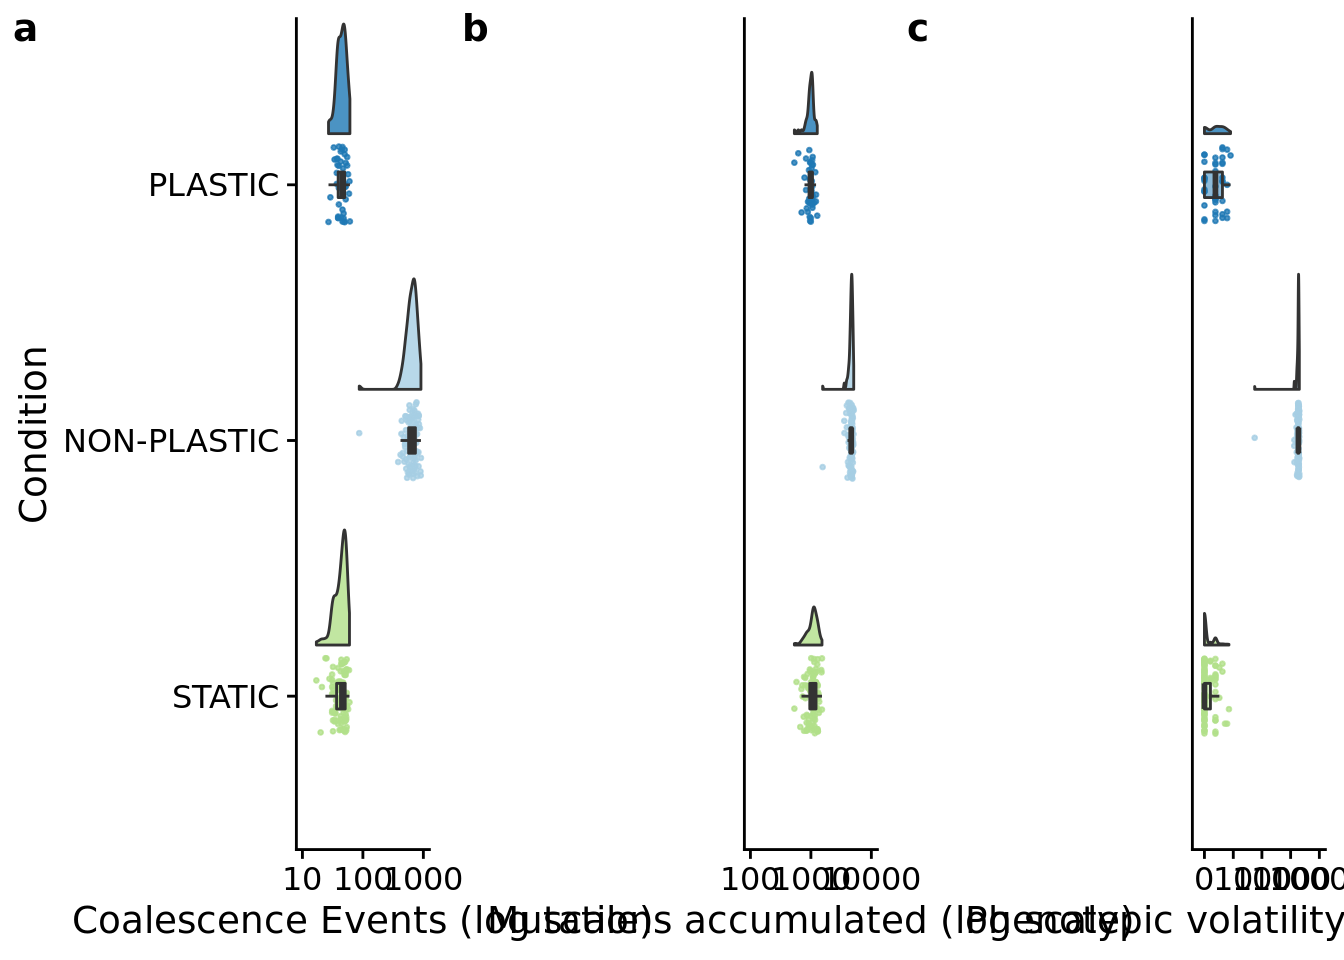
\includegraphics{supplemental-material_files/figure-latex/unnamed-chunk-48-1.pdf}

We can confirm our expectation that the dominant genotypes in non-plastic conditions are not phenotypically plastic.

\begin{Shaded}
\begin{Highlighting}[]
\NormalTok{summary_data_grouped =}\StringTok{ }\NormalTok{dplyr}\OperatorTok{::}\KeywordTok{group_by}\NormalTok{(summary_data, condition, is_plastic, extra_task_value)}
\NormalTok{summary_data_group_counts =}\StringTok{ }\NormalTok{dplyr}\OperatorTok{::}\KeywordTok{summarize}\NormalTok{(summary_data_grouped, }\DataTypeTok{n=}\NormalTok{dplyr}\OperatorTok{::}\KeywordTok{n}\NormalTok{())}
\KeywordTok{ggplot}\NormalTok{(}\KeywordTok{filter}\NormalTok{(summary_data_group_counts, is_plastic), }\KeywordTok{aes}\NormalTok{(}\DataTypeTok{x=}\NormalTok{condition, }\DataTypeTok{y=}\NormalTok{n, }\DataTypeTok{fill=}\NormalTok{condition)) }\OperatorTok{+}
\StringTok{  }\KeywordTok{geom_col}\NormalTok{(}\DataTypeTok{position=}\KeywordTok{position_dodge}\NormalTok{(}\FloatTok{0.9}\NormalTok{)) }\OperatorTok{+}
\StringTok{  }\KeywordTok{scale_x_discrete}\NormalTok{(}
    \DataTypeTok{name=}\StringTok{"Condition"}\NormalTok{,}
    \DataTypeTok{limits=}\NormalTok{condition_order}
\NormalTok{  ) }\OperatorTok{+}
\StringTok{  }\KeywordTok{scale_fill_brewer}\NormalTok{(}
    \DataTypeTok{palette=}\NormalTok{cb_palette}
\NormalTok{  ) }\OperatorTok{+}
\StringTok{  }\KeywordTok{scale_color_brewer}\NormalTok{(}
    \DataTypeTok{palette=}\NormalTok{cb_palette}
\NormalTok{  ) }\OperatorTok{+}
\StringTok{  }\KeywordTok{ylim}\NormalTok{(}\DecValTok{0}\NormalTok{, }\DecValTok{100}\NormalTok{) }\OperatorTok{+}
\StringTok{  }\KeywordTok{geom_text}\NormalTok{(}\KeywordTok{aes}\NormalTok{(}\DataTypeTok{label=}\NormalTok{n, }\DataTypeTok{y=}\NormalTok{n}\OperatorTok{+}\DecValTok{1}\NormalTok{)) }\OperatorTok{+}
\StringTok{  }\KeywordTok{ylab}\NormalTok{(}\StringTok{"Number of replicates with a plastic dominant genotype"}\NormalTok{) }\OperatorTok{+}
\StringTok{  }\KeywordTok{facet_wrap}\NormalTok{(}\OperatorTok{~}\NormalTok{extra_task_value, }\DataTypeTok{labeller=}\NormalTok{label_both) }\OperatorTok{+}
\StringTok{  }\KeywordTok{theme}\NormalTok{(}
    \DataTypeTok{legend.position=}\StringTok{"none"}
\NormalTok{  )}
\end{Highlighting}
\end{Shaded}

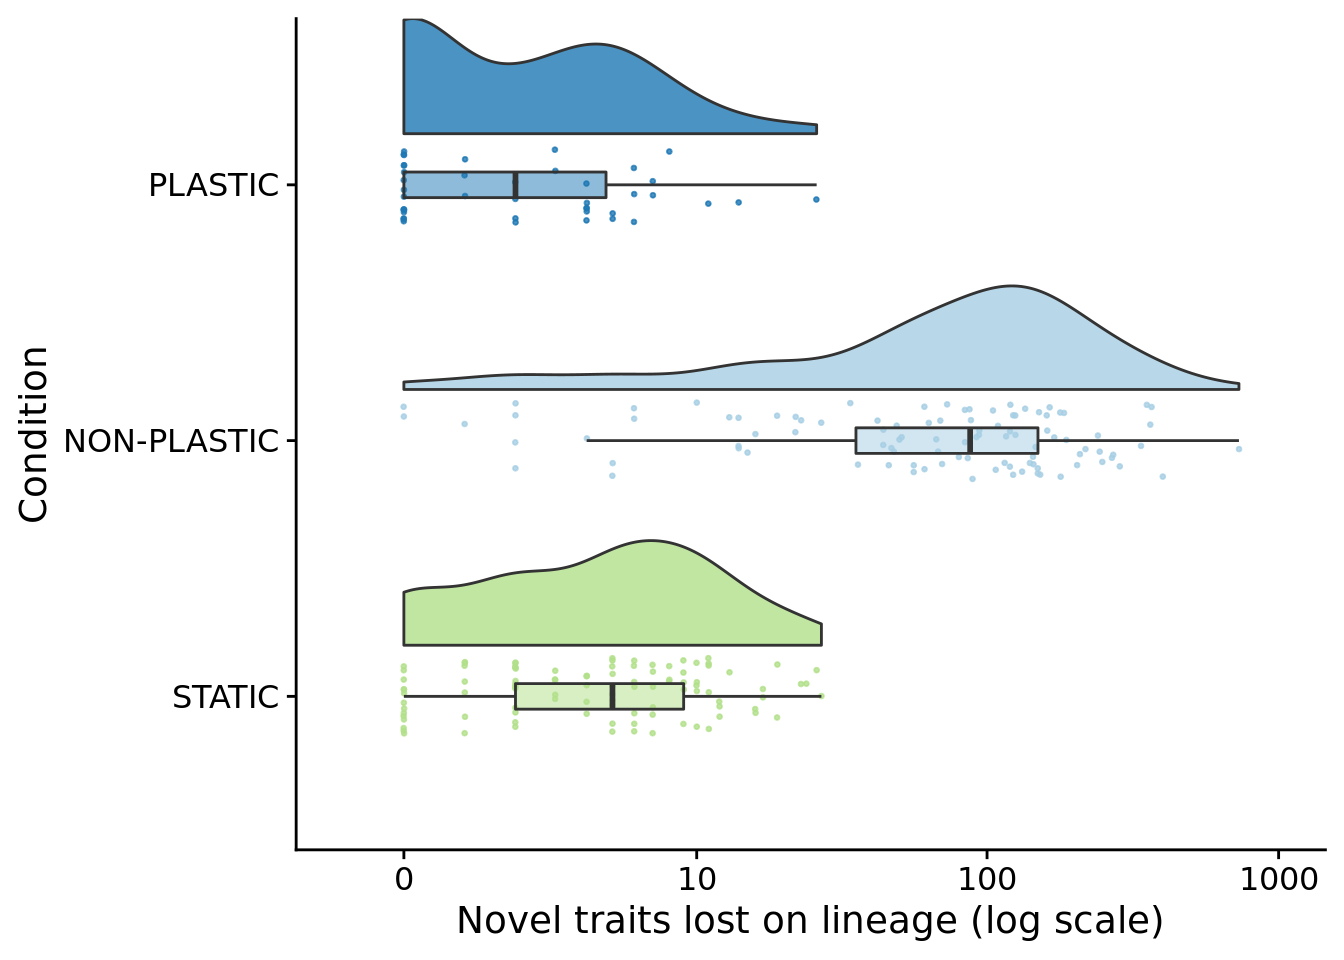
\includegraphics{supplemental-material_files/figure-latex/unnamed-chunk-49-1.pdf}

\hypertarget{final-novel-function-count-dominant-genotype}{%
\section{Final novel function count (dominant genotype)}\label{final-novel-function-count-dominant-genotype}}

How many novel functions do final dominant genotypes perform?

\begin{Shaded}
\begin{Highlighting}[]
\CommentTok{# Compute manual labels for geom_signif}
\NormalTok{stat.test <-}\StringTok{ }\NormalTok{summary_data }\OperatorTok
\StringTok{  }\KeywordTok{wilcox_test}\NormalTok{(dominant_extra_tasks }\OperatorTok{~}\StringTok{ }\NormalTok{condition) }\OperatorTok
\StringTok{  }\KeywordTok{adjust_pvalue}\NormalTok{(}\DataTypeTok{method =} \StringTok{"bonferroni"}\NormalTok{) }\OperatorTok
\StringTok{  }\KeywordTok{add_significance}\NormalTok{() }\OperatorTok
\StringTok{  }\KeywordTok{add_xy_position}\NormalTok{(}\DataTypeTok{x=}\StringTok{"condition"}\NormalTok{) }\CommentTok{# ,step.increase=1}
\CommentTok{# Tweak y.position manually to account for scaled axis (edge case that triggers bad behavior in geom_signif)}
\NormalTok{stat.test}\OperatorTok{$}\NormalTok{manual_position <-}\StringTok{ }\NormalTok{stat.test}\OperatorTok{$}\NormalTok{y.position }\CommentTok{#* c(1.0,1.0,1.03)}
\NormalTok{stat.test}\OperatorTok{$}\NormalTok{label <-}\StringTok{ }\KeywordTok{mapply}\NormalTok{(p_label,stat.test}\OperatorTok{$}\NormalTok{p.adj)}

\NormalTok{summary_data}\OperatorTok{$}\NormalTok{is_outlier <-}\StringTok{ }\KeywordTok{mapply}\NormalTok{(}
\NormalTok{  is_outlier,}
\NormalTok{  summary_data}\OperatorTok{$}\NormalTok{dominant_extra_tasks,}
\NormalTok{  summary_data}\OperatorTok{$}\NormalTok{condition,}
  \DataTypeTok{MoreArgs=}\KeywordTok{list}\NormalTok{(}\DataTypeTok{data=}\NormalTok{summary_data, }\DataTypeTok{column=}\StringTok{"dominant_extra_tasks"}\NormalTok{)}
\NormalTok{)}

\NormalTok{final_novel_task_count_fig <-}\StringTok{ }\KeywordTok{ggplot}\NormalTok{(}
\NormalTok{    summary_data,}
    \KeywordTok{aes}\NormalTok{(}\DataTypeTok{x=}\NormalTok{condition, }\DataTypeTok{y=}\NormalTok{dominant_extra_tasks, }\DataTypeTok{fill=}\NormalTok{condition)}
\NormalTok{  ) }\OperatorTok{+}
\StringTok{  }\KeywordTok{geom_flat_violin}\NormalTok{(}
    \CommentTok{# data=filter(summary_data,is_outlier==FALSE),}
    \DataTypeTok{scale=}\StringTok{"width"}\NormalTok{,}
    \DataTypeTok{position =} \KeywordTok{position_nudge}\NormalTok{(}\DataTypeTok{x =} \FloatTok{.2}\NormalTok{, }\DataTypeTok{y =} \DecValTok{0}\NormalTok{),}
    \DataTypeTok{alpha =} \FloatTok{.8}
\NormalTok{  ) }\OperatorTok{+}
\StringTok{  }\KeywordTok{geom_point}\NormalTok{(}
    \DataTypeTok{mapping=}\KeywordTok{aes}\NormalTok{(}\DataTypeTok{color=}\NormalTok{condition),}
    \DataTypeTok{position =} \KeywordTok{position_jitter}\NormalTok{(}\DataTypeTok{width =} \FloatTok{.15}\NormalTok{),}
    \DataTypeTok{size =} \FloatTok{.5}\NormalTok{,}
    \DataTypeTok{alpha =} \FloatTok{0.8}
\NormalTok{  ) }\OperatorTok{+}
\StringTok{  }\KeywordTok{geom_boxplot}\NormalTok{(}
    \DataTypeTok{width =} \FloatTok{.1}\NormalTok{,}
    \DataTypeTok{outlier.shape =} \OtherTok{NA}\NormalTok{,}
    \DataTypeTok{alpha =} \FloatTok{0.5}
\NormalTok{  ) }\OperatorTok{+}
\StringTok{  }\KeywordTok{scale_x_discrete}\NormalTok{(}
    \DataTypeTok{name=}\StringTok{"Condition"}\NormalTok{,}
    \DataTypeTok{limits=}\NormalTok{condition_order,}
    \DataTypeTok{labels=}\NormalTok{condition_order}
\NormalTok{  ) }\OperatorTok{+}
\StringTok{  }\KeywordTok{scale_y_continuous}\NormalTok{(}
    \DataTypeTok{name=}\StringTok{"Final novel function count"}
\NormalTok{  ) }\OperatorTok{+}
\StringTok{  }\KeywordTok{scale_fill_brewer}\NormalTok{(}
    \DataTypeTok{palette=}\NormalTok{cb_palette}
\NormalTok{  ) }\OperatorTok{+}
\StringTok{  }\KeywordTok{scale_color_brewer}\NormalTok{(}
    \DataTypeTok{palette=}\NormalTok{cb_palette}
\NormalTok{  ) }\OperatorTok{+}
\StringTok{  }\KeywordTok{labs}\NormalTok{(}
    \DataTypeTok{subtitle=}\KeywordTok{paste0}\NormalTok{(}
      \StringTok{"Kruskal-Wallis, "}\NormalTok{,}
      \KeywordTok{p_label}\NormalTok{(}\KeywordTok{signif}\NormalTok{(}\KeywordTok{kruskal.test}\NormalTok{(}\DataTypeTok{formula=}\NormalTok{dominant_extra_tasks}\OperatorTok{~}\NormalTok{condition, }\DataTypeTok{data=}\NormalTok{summary_data)}\OperatorTok{$}\NormalTok{p.value,}\DataTypeTok{digits=}\DecValTok{4}\NormalTok{))}
\NormalTok{    )}
\NormalTok{  ) }\OperatorTok{+}
\StringTok{  }\NormalTok{ggsignif}\OperatorTok{::}\KeywordTok{geom_signif}\NormalTok{(}
    \DataTypeTok{data=}\KeywordTok{filter}\NormalTok{(stat.test, p.adj }\OperatorTok{<=}\StringTok{ }\NormalTok{alpha),}
    \KeywordTok{aes}\NormalTok{(}\DataTypeTok{xmin=}\NormalTok{group1,}\DataTypeTok{xmax=}\NormalTok{group2,}\DataTypeTok{annotations=}\NormalTok{label,}\DataTypeTok{y_position=}\NormalTok{manual_position),}
    \DataTypeTok{manual=}\OtherTok{TRUE}\NormalTok{,}
    \DataTypeTok{inherit.aes=}\OtherTok{FALSE}
\NormalTok{  ) }\OperatorTok{+}
\StringTok{  }\CommentTok{# coord_flip()}
\StringTok{  }\KeywordTok{theme}\NormalTok{(}
    \DataTypeTok{legend.position=}\StringTok{"none"}
\NormalTok{  )}
\end{Highlighting}
\end{Shaded}

\begin{verbatim}
## Warning: Ignoring unknown aesthetics: xmin, xmax, annotations, y_position
\end{verbatim}

\begin{Shaded}
\begin{Highlighting}[]
\NormalTok{final_novel_task_count_fig}
\end{Highlighting}
\end{Shaded}

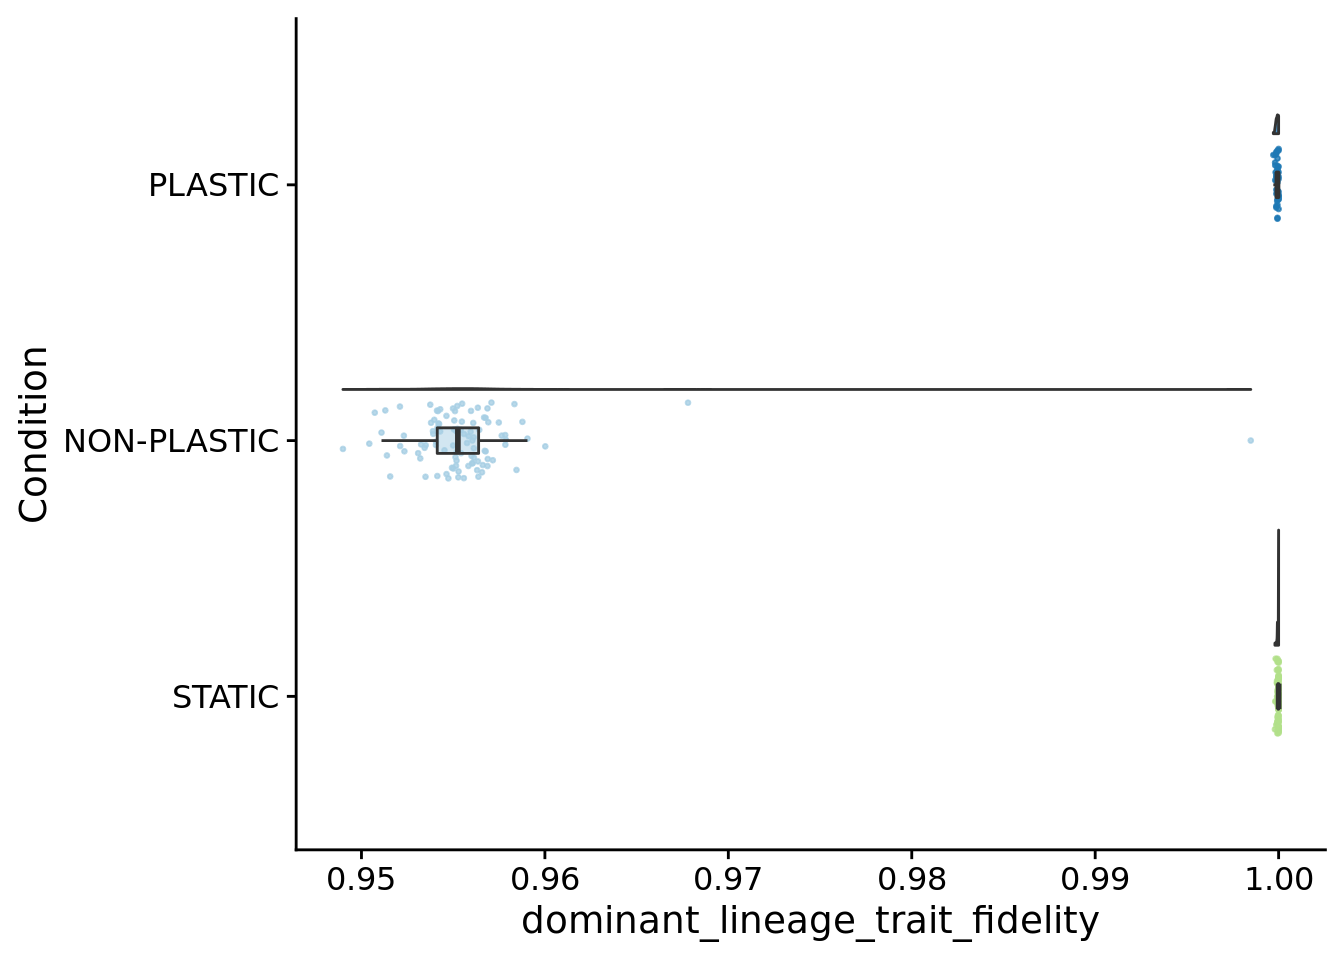
\includegraphics{supplemental-material_files/figure-latex/unnamed-chunk-50-1.pdf}

\begin{Shaded}
\begin{Highlighting}[]
\KeywordTok{kruskal.test}\NormalTok{(}
  \DataTypeTok{formula=}\NormalTok{dominant_extra_tasks}\OperatorTok{~}\NormalTok{condition,}
  \DataTypeTok{data=}\NormalTok{summary_data}
\NormalTok{)}
\end{Highlighting}
\end{Shaded}

\begin{verbatim}
## 
##  Kruskal-Wallis rank sum test
## 
## data:  dominant_extra_tasks by condition
## Kruskal-Wallis chi-squared = 177.17, df = 2, p-value < 2.2e-16
\end{verbatim}

\begin{Shaded}
\begin{Highlighting}[]
\KeywordTok{pairwise.wilcox.test}\NormalTok{(}
  \DataTypeTok{x=}\NormalTok{summary_data}\OperatorTok{$}\NormalTok{dominant_extra_tasks,}
  \DataTypeTok{g=}\NormalTok{summary_data}\OperatorTok{$}\NormalTok{condition,}
  \DataTypeTok{p.adjust.method=}\StringTok{"bonferroni"}\NormalTok{,}
  \DataTypeTok{conf.int=}\OtherTok{TRUE}\NormalTok{,}
  \DataTypeTok{conf.level=}\FloatTok{0.95}
\NormalTok{)}
\end{Highlighting}
\end{Shaded}

\begin{verbatim}
## 
##  Pairwise comparisons using Wilcoxon rank sum test with continuity correction 
## 
## data:  summary_data$dominant_extra_tasks and summary_data$condition 
## 
##         NON-PLASTIC PLASTIC
## PLASTIC <2e-16      -      
## STATIC  <2e-16      0.9    
## 
## P value adjustment method: bonferroni
\end{verbatim}

\begin{Shaded}
\begin{Highlighting}[]
\KeywordTok{paste}\NormalTok{(}
  \DataTypeTok{sep=}\StringTok{"; "}\NormalTok{,}
  \KeywordTok{paste0}\NormalTok{(}
    \StringTok{"PLASTIC median: "}\NormalTok{,}
    \KeywordTok{median}\NormalTok{(}\KeywordTok{filter}\NormalTok{(summary_data, condition}\OperatorTok{==}\StringTok{"PLASTIC"}\NormalTok{)}\OperatorTok{$}\NormalTok{dominant_extra_tasks)}
\NormalTok{  ),}
  \KeywordTok{paste0}\NormalTok{(}
    \StringTok{"STATIC median: "}\NormalTok{,}
    \KeywordTok{median}\NormalTok{(}\KeywordTok{filter}\NormalTok{(summary_data, condition}\OperatorTok{==}\StringTok{"STATIC"}\NormalTok{)}\OperatorTok{$}\NormalTok{dominant_extra_tasks)}
\NormalTok{  ),}
  \KeywordTok{paste0}\NormalTok{(}
    \StringTok{"NON-PLASTIC median: "}\NormalTok{,}
    \KeywordTok{median}\NormalTok{(}\KeywordTok{filter}\NormalTok{(summary_data, condition}\OperatorTok{==}\StringTok{"NON-PLASTIC"}\NormalTok{)}\OperatorTok{$}\NormalTok{dominant_extra_tasks)}
\NormalTok{  )}
\NormalTok{)}
\end{Highlighting}
\end{Shaded}

\begin{verbatim}
## [1] "PLASTIC median: 3; STATIC median: 3; NON-PLASTIC median: 0"
\end{verbatim}

\begin{Shaded}
\begin{Highlighting}[]
\KeywordTok{print}\NormalTok{(}\StringTok{"Wilcox rank sum test statistics:"}\NormalTok{)}
\end{Highlighting}
\end{Shaded}

\begin{verbatim}
## [1] "Wilcox rank sum test statistics:"
\end{verbatim}

\begin{Shaded}
\begin{Highlighting}[]
\ControlFlowTok{for}\NormalTok{ (pair }\ControlFlowTok{in}\NormalTok{ pairwise_comparisons) \{}
\NormalTok{  pair_data <-}\StringTok{ }\KeywordTok{filter}\NormalTok{(summary_data, condition }\OperatorTok\StringTok{ }\NormalTok{pair)}
\NormalTok{  pair_data}\OperatorTok{$}\NormalTok{condition <-}\StringTok{ }\KeywordTok{as.factor}\NormalTok{(pair_data}\OperatorTok{$}\NormalTok{condition)}
\NormalTok{  wt <-}\StringTok{ }\KeywordTok{wilcox.test}\NormalTok{(}
    \DataTypeTok{formula=}\NormalTok{dominant_extra_tasks}\OperatorTok{~}\NormalTok{condition,}
    \DataTypeTok{data=}\NormalTok{pair_data,}
    \DataTypeTok{exact=}\OtherTok{FALSE}\NormalTok{,}
    \DataTypeTok{paired=}\OtherTok{FALSE}
\NormalTok{  )}
  \KeywordTok{print}\NormalTok{(}\KeywordTok{paste0}\NormalTok{(pair[}\DecValTok{1}\NormalTok{], }\StringTok{"<-->"}\NormalTok{, pair[}\DecValTok{2}\NormalTok{], }\StringTok{": W="}\NormalTok{,wt}\OperatorTok{$}\NormalTok{statistic))}
\NormalTok{\}}
\end{Highlighting}
\end{Shaded}

\begin{verbatim}
## [1] "STATIC<-->NON-PLASTIC: W=184"
## [1] "STATIC<-->PLASTIC: W=1871"
## [1] "PLASTIC<-->NON-PLASTIC: W=64"
\end{verbatim}

\hypertarget{novel-function-count-final-population}{%
\section{Novel function count (final population)}\label{novel-function-count-final-population}}

How many novel functions are performed across the final population (1\% of organisms must perform to count)?

\begin{Shaded}
\begin{Highlighting}[]
\KeywordTok{ggplot}\NormalTok{(summary_data, }\KeywordTok{aes}\NormalTok{(}\DataTypeTok{x=}\NormalTok{condition, }\DataTypeTok{y=}\NormalTok{final_pop_extra_tasks_}\FloatTok{0.01}\NormalTok{, }\DataTypeTok{fill=}\NormalTok{condition)) }\OperatorTok{+}
\StringTok{  }\KeywordTok{geom_flat_violin}\NormalTok{(}
    \DataTypeTok{position =} \KeywordTok{position_nudge}\NormalTok{(}\DataTypeTok{x =} \FloatTok{.2}\NormalTok{, }\DataTypeTok{y =} \DecValTok{0}\NormalTok{),}
    \DataTypeTok{alpha =} \FloatTok{.8}
\NormalTok{  ) }\OperatorTok{+}
\StringTok{  }\KeywordTok{geom_point}\NormalTok{(}
    \DataTypeTok{mapping=}\KeywordTok{aes}\NormalTok{(}\DataTypeTok{color=}\NormalTok{condition),}
    \DataTypeTok{position =} \KeywordTok{position_jitter}\NormalTok{(}\DataTypeTok{width =} \FloatTok{.15}\NormalTok{),}
    \DataTypeTok{size =} \FloatTok{.5}\NormalTok{,}
    \DataTypeTok{alpha =} \FloatTok{0.8}
\NormalTok{  ) }\OperatorTok{+}
\StringTok{  }\KeywordTok{geom_boxplot}\NormalTok{(}
    \DataTypeTok{width =} \FloatTok{.1}\NormalTok{,}
    \DataTypeTok{outlier.shape =} \OtherTok{NA}\NormalTok{,}
    \DataTypeTok{alpha =} \FloatTok{0.5}
\NormalTok{  ) }\OperatorTok{+}
\StringTok{  }\KeywordTok{scale_x_discrete}\NormalTok{(}
    \DataTypeTok{name=}\StringTok{"Condition"}\NormalTok{,}
    \DataTypeTok{limits=}\NormalTok{condition_order}
\NormalTok{  ) }\OperatorTok{+}
\StringTok{  }\KeywordTok{scale_fill_brewer}\NormalTok{(}
    \DataTypeTok{palette=}\NormalTok{cb_palette}
\NormalTok{  ) }\OperatorTok{+}
\StringTok{  }\KeywordTok{scale_color_brewer}\NormalTok{(}
    \DataTypeTok{palette=}\NormalTok{cb_palette}
\NormalTok{  ) }\OperatorTok{+}
\StringTok{  }\CommentTok{# coord_flip() +}
\StringTok{  }\KeywordTok{theme}\NormalTok{(}
    \DataTypeTok{legend.position=}\StringTok{"none"}
\NormalTok{  )}
\end{Highlighting}
\end{Shaded}

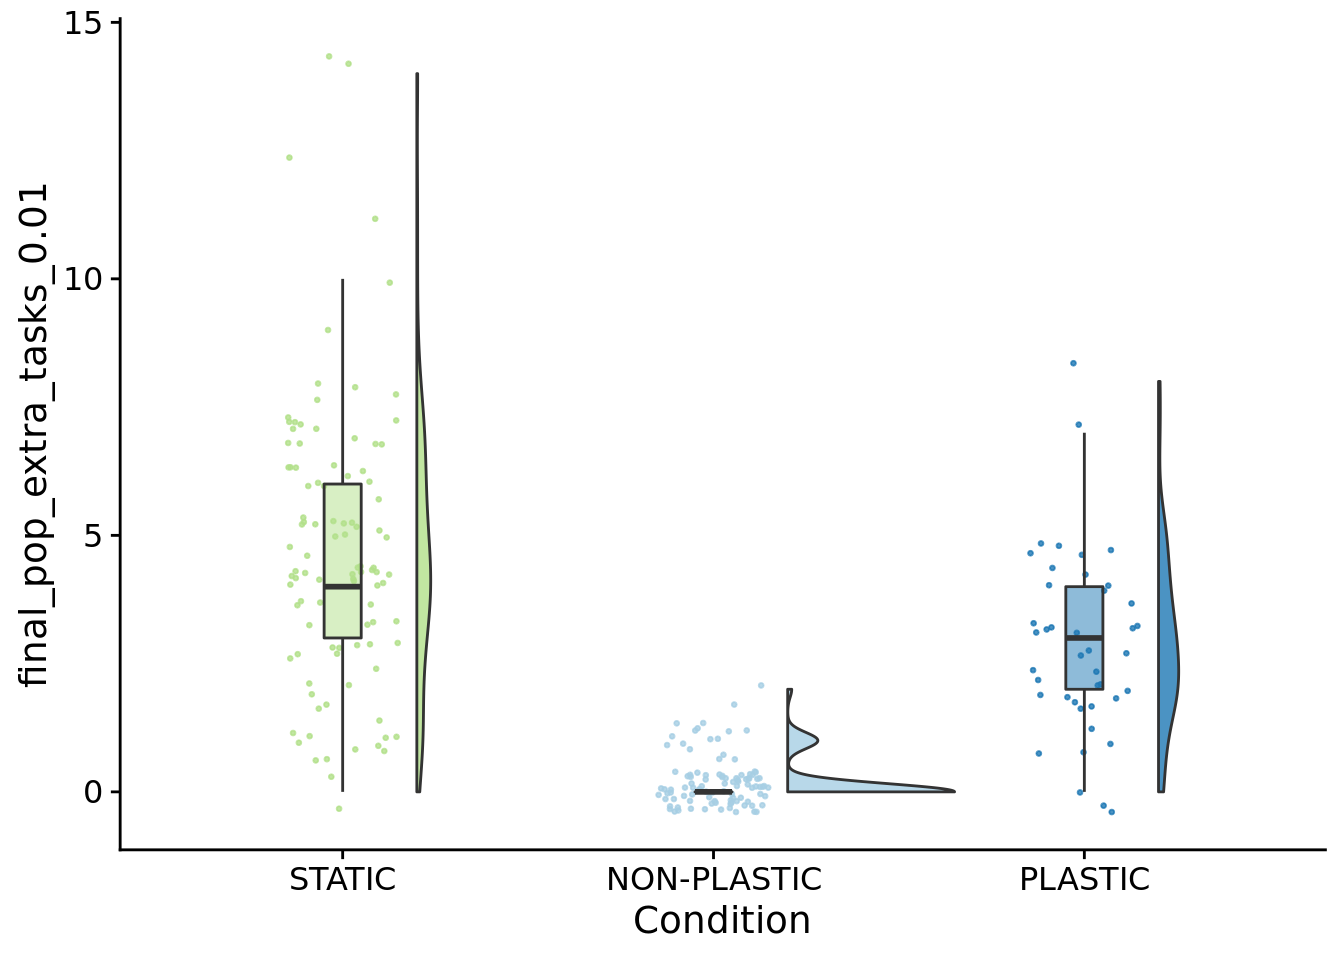
\includegraphics{supplemental-material_files/figure-latex/unnamed-chunk-52-1.pdf}

\begin{Shaded}
\begin{Highlighting}[]
\KeywordTok{kruskal.test}\NormalTok{(}
  \DataTypeTok{formula=}\NormalTok{final_pop_extra_tasks_}\FloatTok{0.01}\OperatorTok{~}\NormalTok{condition,}
  \DataTypeTok{data=}\NormalTok{summary_data}
\NormalTok{)}
\end{Highlighting}
\end{Shaded}

\begin{verbatim}
## 
##  Kruskal-Wallis rank sum test
## 
## data:  final_pop_extra_tasks_0.01 by condition
## Kruskal-Wallis chi-squared = 169.47, df = 2, p-value < 2.2e-16
\end{verbatim}

\begin{Shaded}
\begin{Highlighting}[]
\KeywordTok{pairwise.wilcox.test}\NormalTok{(}
  \DataTypeTok{x=}\NormalTok{summary_data}\OperatorTok{$}\NormalTok{final_pop_extra_tasks_}\FloatTok{0.01}\NormalTok{,}
  \DataTypeTok{g=}\NormalTok{summary_data}\OperatorTok{$}\NormalTok{condition,}
  \DataTypeTok{p.adjust.method=}\StringTok{"bonferroni"}\NormalTok{,}
  \DataTypeTok{conf.int=}\OtherTok{TRUE}\NormalTok{,}
  \DataTypeTok{conf.level=}\FloatTok{0.95}
\NormalTok{)}
\end{Highlighting}
\end{Shaded}

\begin{verbatim}
## 
##  Pairwise comparisons using Wilcoxon rank sum test with continuity correction 
## 
## data:  summary_data$final_pop_extra_tasks_0.01 and summary_data$condition 
## 
##         NON-PLASTIC PLASTIC
## PLASTIC < 2e-16     -      
## STATIC  < 2e-16     0.00016
## 
## P value adjustment method: bonferroni
\end{verbatim}

\begin{Shaded}
\begin{Highlighting}[]
\KeywordTok{paste}\NormalTok{(}
  \DataTypeTok{sep=}\StringTok{"; "}\NormalTok{,}
  \KeywordTok{paste0}\NormalTok{(}
    \StringTok{"PLASTIC median: "}\NormalTok{,}
    \KeywordTok{median}\NormalTok{(}\KeywordTok{filter}\NormalTok{(summary_data, condition}\OperatorTok{==}\StringTok{"PLASTIC"}\NormalTok{)}\OperatorTok{$}\NormalTok{final_pop_extra_tasks_}\FloatTok{0.01}\NormalTok{)}
\NormalTok{  ),}
  \KeywordTok{paste0}\NormalTok{(}
    \StringTok{"STATIC median: "}\NormalTok{,}
    \KeywordTok{median}\NormalTok{(}\KeywordTok{filter}\NormalTok{(summary_data, condition}\OperatorTok{==}\StringTok{"STATIC"}\NormalTok{)}\OperatorTok{$}\NormalTok{final_pop_extra_tasks_}\FloatTok{0.01}\NormalTok{)}
\NormalTok{  ),}
  \KeywordTok{paste0}\NormalTok{(}
    \StringTok{"NON-PLASTIC median: "}\NormalTok{,}
    \KeywordTok{median}\NormalTok{(}\KeywordTok{filter}\NormalTok{(summary_data, condition}\OperatorTok{==}\StringTok{"NON-PLASTIC"}\NormalTok{)}\OperatorTok{$}\NormalTok{final_pop_extra_tasks_}\FloatTok{0.01}\NormalTok{)}
\NormalTok{  )}
\NormalTok{)}
\end{Highlighting}
\end{Shaded}

\begin{verbatim}
## [1] "PLASTIC median: 3; STATIC median: 4; NON-PLASTIC median: 0"
\end{verbatim}

\begin{Shaded}
\begin{Highlighting}[]
\KeywordTok{print}\NormalTok{(}\StringTok{"Wilcox rank sum test statistics:"}\NormalTok{)}
\end{Highlighting}
\end{Shaded}

\begin{verbatim}
## [1] "Wilcox rank sum test statistics:"
\end{verbatim}

\begin{Shaded}
\begin{Highlighting}[]
\ControlFlowTok{for}\NormalTok{ (pair }\ControlFlowTok{in}\NormalTok{ pairwise_comparisons) \{}
\NormalTok{  pair_data <-}\StringTok{ }\KeywordTok{filter}\NormalTok{(summary_data, condition }\OperatorTok\StringTok{ }\NormalTok{pair)}
\NormalTok{  pair_data}\OperatorTok{$}\NormalTok{condition <-}\StringTok{ }\KeywordTok{as.factor}\NormalTok{(pair_data}\OperatorTok{$}\NormalTok{condition)}
\NormalTok{  wt <-}\StringTok{ }\KeywordTok{wilcox.test}\NormalTok{(}
    \DataTypeTok{formula=}\NormalTok{final_pop_extra_tasks_}\FloatTok{0.01}\OperatorTok{~}\NormalTok{condition,}
    \DataTypeTok{data=}\NormalTok{pair_data,}
    \DataTypeTok{exact=}\OtherTok{FALSE}\NormalTok{,}
    \DataTypeTok{paired=}\OtherTok{FALSE}
\NormalTok{  )}
  \KeywordTok{print}\NormalTok{(}\KeywordTok{paste0}\NormalTok{(pair[}\DecValTok{1}\NormalTok{], }\StringTok{"<-->"}\NormalTok{, pair[}\DecValTok{2}\NormalTok{], }\StringTok{": W="}\NormalTok{,wt}\OperatorTok{$}\NormalTok{statistic))}
\NormalTok{\}}
\end{Highlighting}
\end{Shaded}

\begin{verbatim}
## [1] "STATIC<-->NON-PLASTIC: W=227.5"
## [1] "STATIC<-->PLASTIC: W=1203"
## [1] "PLASTIC<-->NON-PLASTIC: W=225.5"
\end{verbatim}

\hypertarget{novel-function-discovery-lineage}{%
\section{Novel function discovery (lineage)}\label{novel-function-discovery-lineage}}

\begin{Shaded}
\begin{Highlighting}[]
\CommentTok{# Compute manual labels for geom_signif}
\NormalTok{stat.test <-}\StringTok{ }\NormalTok{summary_data }\OperatorTok
\StringTok{  }\KeywordTok{wilcox_test}\NormalTok{(dominant_lineage_extra_traits_discovered }\OperatorTok{~}\StringTok{ }\NormalTok{condition) }\OperatorTok
\StringTok{  }\KeywordTok{adjust_pvalue}\NormalTok{(}\DataTypeTok{method =} \StringTok{"bonferroni"}\NormalTok{) }\OperatorTok
\StringTok{  }\KeywordTok{add_significance}\NormalTok{() }\OperatorTok
\StringTok{  }\KeywordTok{add_xy_position}\NormalTok{(}\DataTypeTok{x=}\StringTok{"condition"}\NormalTok{) }\CommentTok{# ,step.increase=1}
\CommentTok{# Tweak y.position manually to account for scaled axis (edge case that triggers bad behavior in geom_signif)}
\NormalTok{stat.test}\OperatorTok{$}\NormalTok{manual_position <-}\StringTok{ }\NormalTok{stat.test}\OperatorTok{$}\NormalTok{y.position }\CommentTok{#* c(1.0,1.0,1.03)}
\NormalTok{stat.test}\OperatorTok{$}\NormalTok{label <-}\StringTok{ }\KeywordTok{mapply}\NormalTok{(p_label,stat.test}\OperatorTok{$}\NormalTok{p.adj)}

\NormalTok{summary_data}\OperatorTok{$}\NormalTok{is_outlier <-}\StringTok{ }\KeywordTok{mapply}\NormalTok{(}
\NormalTok{  is_outlier,}
\NormalTok{  summary_data}\OperatorTok{$}\NormalTok{dominant_lineage_extra_traits_discovered,}
\NormalTok{  summary_data}\OperatorTok{$}\NormalTok{condition,}
  \DataTypeTok{MoreArgs=}\KeywordTok{list}\NormalTok{(}\DataTypeTok{data=}\NormalTok{summary_data, }\DataTypeTok{column=}\StringTok{"dominant_lineage_extra_traits_discovered"}\NormalTok{)}
\NormalTok{)}

\NormalTok{lineage_novel_task_discovery_fig <-}\StringTok{ }\KeywordTok{ggplot}\NormalTok{(}
\NormalTok{    summary_data,}
    \KeywordTok{aes}\NormalTok{(}\DataTypeTok{x=}\NormalTok{condition, }\DataTypeTok{y=}\NormalTok{dominant_lineage_extra_traits_discovered, }\DataTypeTok{fill=}\NormalTok{condition)}
\NormalTok{  ) }\OperatorTok{+}
\StringTok{  }\KeywordTok{geom_flat_violin}\NormalTok{(}
    \CommentTok{# data=filter(summary_data,is_outlier==FALSE),}
    \DataTypeTok{scale=}\StringTok{"width"}\NormalTok{,}
    \DataTypeTok{position =} \KeywordTok{position_nudge}\NormalTok{(}\DataTypeTok{x =} \FloatTok{.2}\NormalTok{, }\DataTypeTok{y =} \DecValTok{0}\NormalTok{),}
    \DataTypeTok{alpha =} \FloatTok{.8}
\NormalTok{  ) }\OperatorTok{+}
\StringTok{  }\KeywordTok{geom_point}\NormalTok{(}
    \DataTypeTok{mapping=}\KeywordTok{aes}\NormalTok{(}\DataTypeTok{color=}\NormalTok{condition),}
    \DataTypeTok{position =} \KeywordTok{position_jitter}\NormalTok{(}\DataTypeTok{width =} \FloatTok{.15}\NormalTok{),}
    \DataTypeTok{size =} \FloatTok{.5}\NormalTok{,}
    \DataTypeTok{alpha =} \FloatTok{0.8}
\NormalTok{  ) }\OperatorTok{+}
\StringTok{  }\KeywordTok{geom_boxplot}\NormalTok{(}
    \DataTypeTok{width =} \FloatTok{.1}\NormalTok{,}
    \DataTypeTok{outlier.shape =} \OtherTok{NA}\NormalTok{,}
    \DataTypeTok{alpha =} \FloatTok{0.5}
\NormalTok{  ) }\OperatorTok{+}
\StringTok{  }\KeywordTok{scale_x_discrete}\NormalTok{(}
    \DataTypeTok{name=}\StringTok{"Condition"}\NormalTok{,}
    \DataTypeTok{limits=}\NormalTok{condition_order,}
    \DataTypeTok{labels=}\NormalTok{condition_order}
\NormalTok{  ) }\OperatorTok{+}
\StringTok{  }\KeywordTok{scale_y_continuous}\NormalTok{(}
    \DataTypeTok{name=}\StringTok{"Novel function discovery"}
\NormalTok{  ) }\OperatorTok{+}
\StringTok{  }\KeywordTok{scale_fill_brewer}\NormalTok{(}
    \DataTypeTok{palette=}\NormalTok{cb_palette}
\NormalTok{  ) }\OperatorTok{+}
\StringTok{  }\KeywordTok{scale_color_brewer}\NormalTok{(}
    \DataTypeTok{palette=}\NormalTok{cb_palette}
\NormalTok{  ) }\OperatorTok{+}
\StringTok{  }\KeywordTok{labs}\NormalTok{(}
    \DataTypeTok{subtitle=}\KeywordTok{paste0}\NormalTok{(}
      \StringTok{"Kruskal-Wallis, "}\NormalTok{,}
      \KeywordTok{p_label}\NormalTok{(}\KeywordTok{signif}\NormalTok{(}\KeywordTok{kruskal.test}\NormalTok{(}\DataTypeTok{formula=}\NormalTok{dominant_lineage_extra_traits_discovered}\OperatorTok{~}\NormalTok{condition, }\DataTypeTok{data=}\NormalTok{summary_data)}\OperatorTok{$}\NormalTok{p.value,}\DataTypeTok{digits=}\DecValTok{4}\NormalTok{))}
\NormalTok{    )}
\NormalTok{  ) }\OperatorTok{+}
\StringTok{  }\NormalTok{ggsignif}\OperatorTok{::}\KeywordTok{geom_signif}\NormalTok{(}
    \DataTypeTok{data=}\KeywordTok{filter}\NormalTok{(stat.test, p.adj }\OperatorTok{<=}\StringTok{ }\NormalTok{alpha),}
    \KeywordTok{aes}\NormalTok{(}\DataTypeTok{xmin=}\NormalTok{group1,}\DataTypeTok{xmax=}\NormalTok{group2,}\DataTypeTok{annotations=}\NormalTok{label,}\DataTypeTok{y_position=}\NormalTok{manual_position),}
    \DataTypeTok{manual=}\OtherTok{TRUE}\NormalTok{,}
    \DataTypeTok{inherit.aes=}\OtherTok{FALSE}
\NormalTok{  ) }\OperatorTok{+}
\StringTok{  }\CommentTok{# coord_flip()}
\StringTok{  }\KeywordTok{theme}\NormalTok{(}
    \DataTypeTok{legend.position=}\StringTok{"none"}
\NormalTok{  )}
\end{Highlighting}
\end{Shaded}

\begin{verbatim}
## Warning: Ignoring unknown aesthetics: xmin, xmax, annotations, y_position
\end{verbatim}

\begin{Shaded}
\begin{Highlighting}[]
\NormalTok{lineage_novel_task_discovery_fig}
\end{Highlighting}
\end{Shaded}

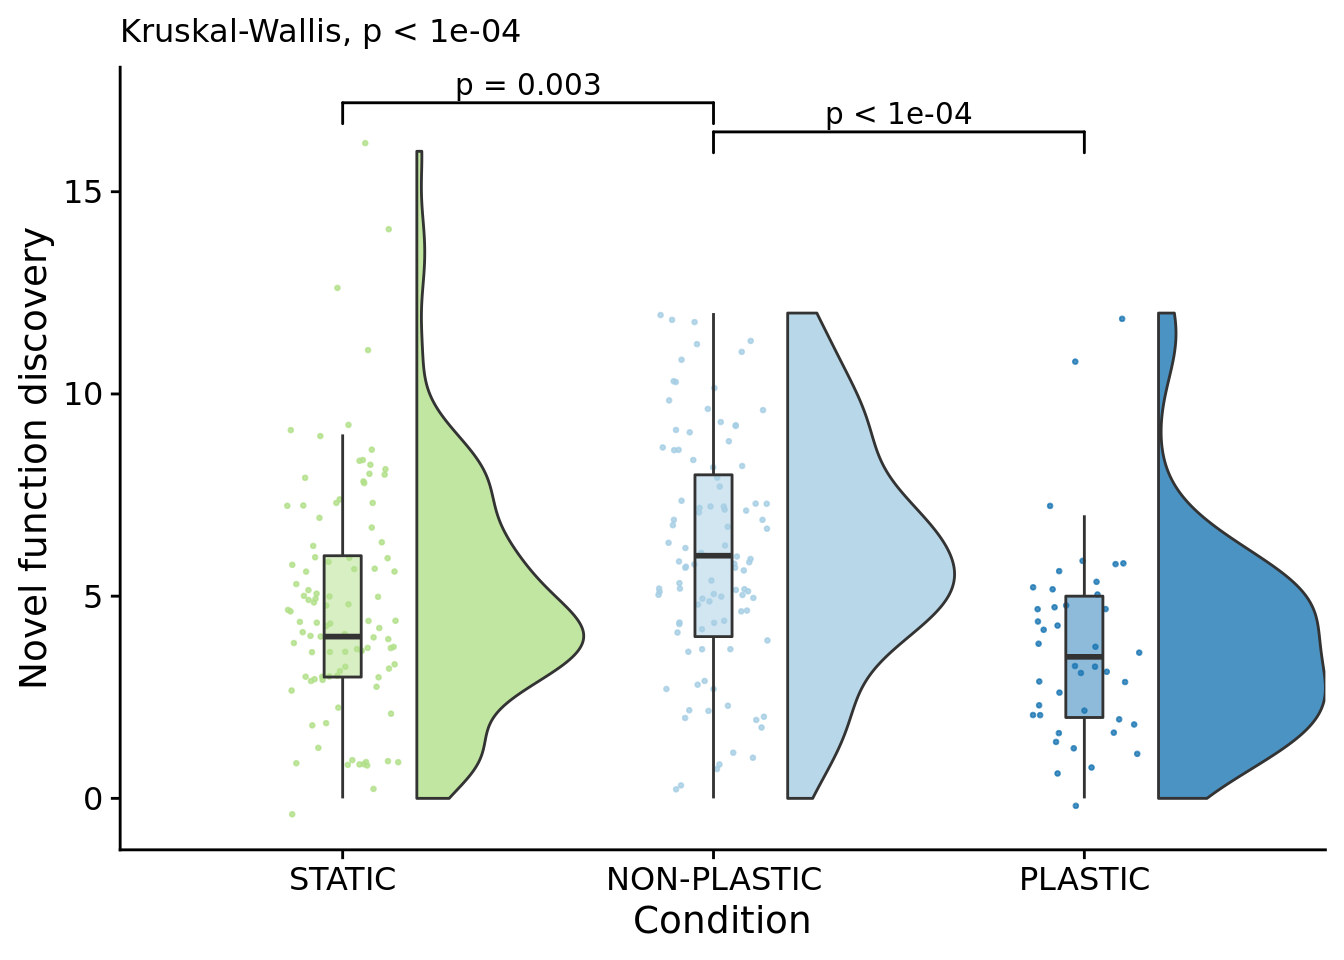
\includegraphics{supplemental-material_files/figure-latex/unnamed-chunk-54-1.pdf}

\begin{Shaded}
\begin{Highlighting}[]
\KeywordTok{kruskal.test}\NormalTok{(}
  \DataTypeTok{formula=}\NormalTok{dominant_lineage_extra_traits_discovered}\OperatorTok{~}\NormalTok{condition,}
  \DataTypeTok{data=}\NormalTok{summary_data}
\NormalTok{)}
\end{Highlighting}
\end{Shaded}

\begin{verbatim}
## 
##  Kruskal-Wallis rank sum test
## 
## data:  dominant_lineage_extra_traits_discovered by condition
## Kruskal-Wallis chi-squared = 24.099, df = 2, p-value = 5.846e-06
\end{verbatim}

\begin{Shaded}
\begin{Highlighting}[]
\KeywordTok{pairwise.wilcox.test}\NormalTok{(}
  \DataTypeTok{x=}\NormalTok{summary_data}\OperatorTok{$}\NormalTok{dominant_lineage_extra_traits_discovered,}
  \DataTypeTok{g=}\NormalTok{summary_data}\OperatorTok{$}\NormalTok{condition,}
  \DataTypeTok{p.adjust.method=}\StringTok{"bonferroni"}\NormalTok{,}
  \DataTypeTok{conf.int=}\OtherTok{TRUE}\NormalTok{,}
  \DataTypeTok{conf.level=}\FloatTok{0.95}
\NormalTok{)}
\end{Highlighting}
\end{Shaded}

\begin{verbatim}
## 
##  Pairwise comparisons using Wilcoxon rank sum test with continuity correction 
## 
## data:  summary_data$dominant_lineage_extra_traits_discovered and summary_data$condition 
## 
##         NON-PLASTIC PLASTIC
## PLASTIC 1.7e-05     -      
## STATIC  0.0035      0.0561 
## 
## P value adjustment method: bonferroni
\end{verbatim}

\begin{Shaded}
\begin{Highlighting}[]
\KeywordTok{paste}\NormalTok{(}
  \DataTypeTok{sep=}\StringTok{"; "}\NormalTok{,}
  \KeywordTok{paste0}\NormalTok{(}
    \StringTok{"PLASTIC median: "}\NormalTok{,}
    \KeywordTok{median}\NormalTok{(}\KeywordTok{filter}\NormalTok{(summary_data, condition}\OperatorTok{==}\StringTok{"PLASTIC"}\NormalTok{)}\OperatorTok{$}\NormalTok{dominant_lineage_extra_traits_discovered)}
\NormalTok{  ),}
  \KeywordTok{paste0}\NormalTok{(}
    \StringTok{"STATIC median: "}\NormalTok{,}
    \KeywordTok{median}\NormalTok{(}\KeywordTok{filter}\NormalTok{(summary_data, condition}\OperatorTok{==}\StringTok{"STATIC"}\NormalTok{)}\OperatorTok{$}\NormalTok{dominant_lineage_extra_traits_discovered)}
\NormalTok{  ),}
  \KeywordTok{paste0}\NormalTok{(}
    \StringTok{"NON-PLASTIC median: "}\NormalTok{,}
    \KeywordTok{median}\NormalTok{(}\KeywordTok{filter}\NormalTok{(summary_data, condition}\OperatorTok{==}\StringTok{"NON-PLASTIC"}\NormalTok{)}\OperatorTok{$}\NormalTok{dominant_lineage_extra_traits_discovered)}
\NormalTok{  )}
\NormalTok{)}
\end{Highlighting}
\end{Shaded}

\begin{verbatim}
## [1] "PLASTIC median: 3.5; STATIC median: 4; NON-PLASTIC median: 6"
\end{verbatim}

\begin{Shaded}
\begin{Highlighting}[]
\KeywordTok{print}\NormalTok{(}\StringTok{"Wilcox rank sum test statistics:"}\NormalTok{)}
\end{Highlighting}
\end{Shaded}

\begin{verbatim}
## [1] "Wilcox rank sum test statistics:"
\end{verbatim}

\begin{Shaded}
\begin{Highlighting}[]
\ControlFlowTok{for}\NormalTok{ (pair }\ControlFlowTok{in}\NormalTok{ pairwise_comparisons) \{}
\NormalTok{  pair_data <-}\StringTok{ }\KeywordTok{filter}\NormalTok{(summary_data, condition }\OperatorTok\StringTok{ }\NormalTok{pair)}
\NormalTok{  pair_data}\OperatorTok{$}\NormalTok{condition <-}\StringTok{ }\KeywordTok{as.factor}\NormalTok{(pair_data}\OperatorTok{$}\NormalTok{condition)}
\NormalTok{  wt <-}\StringTok{ }\KeywordTok{wilcox.test}\NormalTok{(}
    \DataTypeTok{formula=}\NormalTok{dominant_lineage_extra_traits_discovered}\OperatorTok{~}\NormalTok{condition,}
    \DataTypeTok{data=}\NormalTok{pair_data,}
    \DataTypeTok{exact=}\OtherTok{FALSE}\NormalTok{,}
    \DataTypeTok{paired=}\OtherTok{FALSE}
\NormalTok{  )}
  \KeywordTok{print}\NormalTok{(}\KeywordTok{paste0}\NormalTok{(pair[}\DecValTok{1}\NormalTok{], }\StringTok{"<-->"}\NormalTok{, pair[}\DecValTok{2}\NormalTok{], }\StringTok{": W="}\NormalTok{,wt}\OperatorTok{$}\NormalTok{statistic))}
\NormalTok{\}}
\end{Highlighting}
\end{Shaded}

\begin{verbatim}
## [1] "STATIC<-->NON-PLASTIC: W=6319.5"
## [1] "STATIC<-->PLASTIC: W=1578"
## [1] "PLASTIC<-->NON-PLASTIC: W=3110.5"
\end{verbatim}

\hypertarget{novel-function-discovery-population}{%
\section{Novel function discovery (population)}\label{novel-function-discovery-population}}

\begin{Shaded}
\begin{Highlighting}[]
\KeywordTok{ggplot}\NormalTok{(}
\NormalTok{    summary_data,}
    \KeywordTok{aes}\NormalTok{(}\DataTypeTok{x=}\NormalTok{condition, }\DataTypeTok{y=}\NormalTok{discovered_extra_tasks_}\FloatTok{0.01}\NormalTok{, }\DataTypeTok{fill=}\NormalTok{condition)}
\NormalTok{  ) }\OperatorTok{+}
\StringTok{  }\KeywordTok{geom_flat_violin}\NormalTok{(}
    \DataTypeTok{position =} \KeywordTok{position_nudge}\NormalTok{(}\DataTypeTok{x =} \FloatTok{.2}\NormalTok{, }\DataTypeTok{y =} \DecValTok{0}\NormalTok{),}
    \DataTypeTok{alpha =} \FloatTok{.8}
\NormalTok{  ) }\OperatorTok{+}
\StringTok{  }\KeywordTok{geom_point}\NormalTok{(}
    \DataTypeTok{mapping=}\KeywordTok{aes}\NormalTok{(}\DataTypeTok{color=}\NormalTok{condition),}
    \DataTypeTok{position =} \KeywordTok{position_jitter}\NormalTok{(}\DataTypeTok{width =} \FloatTok{.15}\NormalTok{),}
    \DataTypeTok{size =} \FloatTok{.5}\NormalTok{,}
    \DataTypeTok{alpha =} \FloatTok{0.8}
\NormalTok{  ) }\OperatorTok{+}
\StringTok{  }\KeywordTok{geom_boxplot}\NormalTok{(}
    \DataTypeTok{width =} \FloatTok{.1}\NormalTok{,}
    \DataTypeTok{outlier.shape =} \OtherTok{NA}\NormalTok{,}
    \DataTypeTok{alpha =} \FloatTok{0.5}
\NormalTok{  ) }\OperatorTok{+}
\StringTok{  }\KeywordTok{scale_x_discrete}\NormalTok{(}
    \DataTypeTok{name=}\StringTok{"Condition"}\NormalTok{,}
    \DataTypeTok{limits=}\NormalTok{condition_order}
\NormalTok{  ) }\OperatorTok{+}
\StringTok{  }\KeywordTok{scale_fill_brewer}\NormalTok{(}
    \DataTypeTok{palette=}\NormalTok{cb_palette}
\NormalTok{  ) }\OperatorTok{+}
\StringTok{  }\KeywordTok{scale_color_brewer}\NormalTok{(}
    \DataTypeTok{palette=}\NormalTok{cb_palette}
\NormalTok{  ) }\OperatorTok{+}
\StringTok{  }\CommentTok{# coord_flip() +}
\StringTok{  }\KeywordTok{theme}\NormalTok{(}
    \DataTypeTok{legend.position=}\StringTok{"none"}
\NormalTok{  )}
\end{Highlighting}
\end{Shaded}

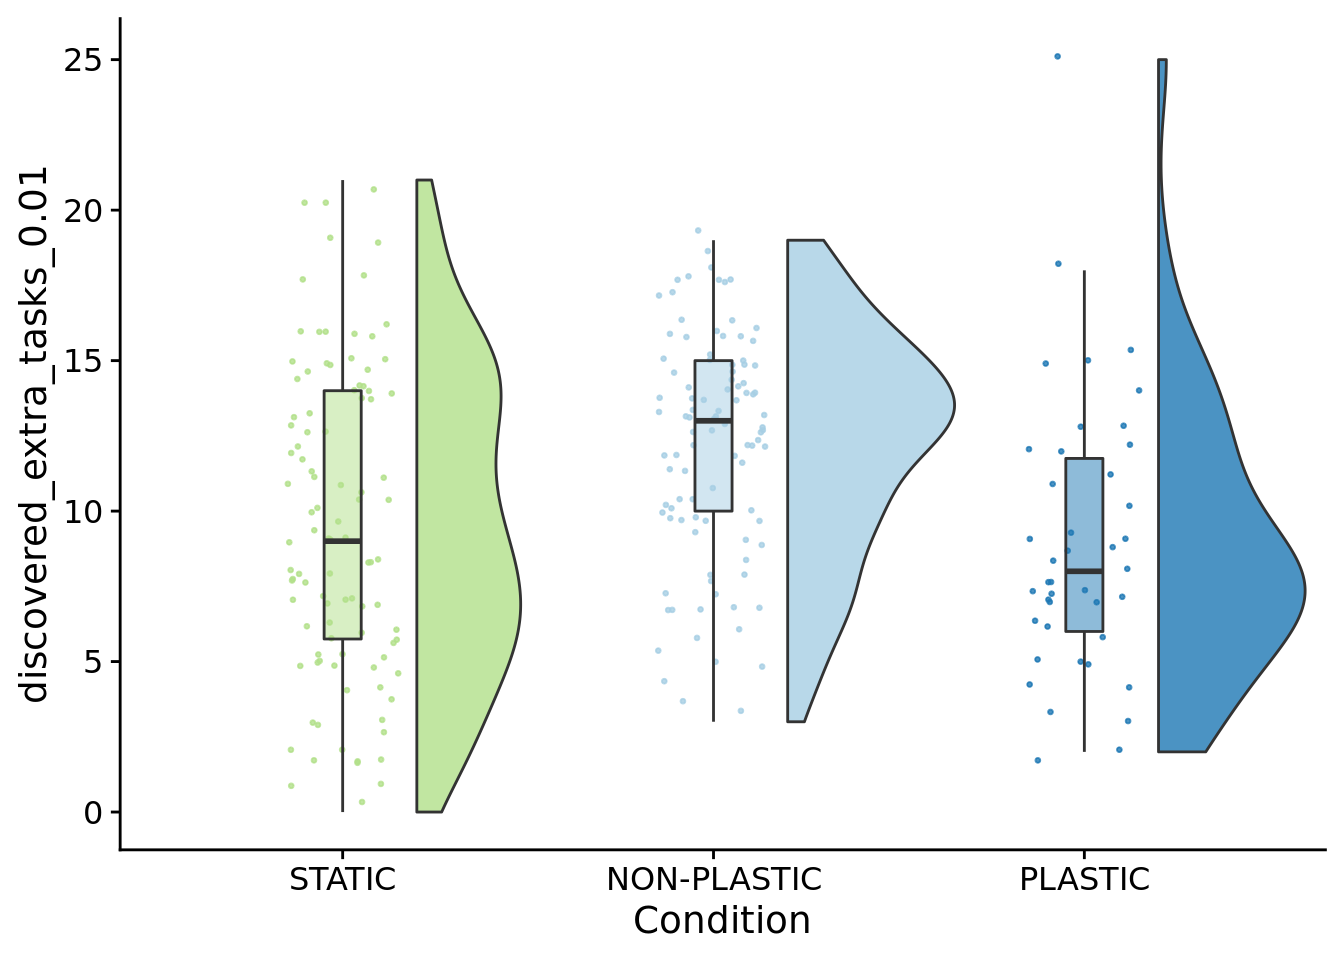
\includegraphics{supplemental-material_files/figure-latex/unnamed-chunk-56-1.pdf}

\begin{Shaded}
\begin{Highlighting}[]
\KeywordTok{kruskal.test}\NormalTok{(}
  \DataTypeTok{formula=}\NormalTok{discovered_extra_tasks_}\FloatTok{0.01}\OperatorTok{~}\NormalTok{condition,}
  \DataTypeTok{data=}\NormalTok{summary_data}
\NormalTok{)}
\end{Highlighting}
\end{Shaded}

\begin{verbatim}
## 
##  Kruskal-Wallis rank sum test
## 
## data:  discovered_extra_tasks_0.01 by condition
## Kruskal-Wallis chi-squared = 24.271, df = 2, p-value = 5.365e-06
\end{verbatim}

\begin{Shaded}
\begin{Highlighting}[]
\KeywordTok{pairwise.wilcox.test}\NormalTok{(}
  \DataTypeTok{x=}\NormalTok{summary_data}\OperatorTok{$}\NormalTok{discovered_extra_tasks_}\FloatTok{0.01}\NormalTok{,}
  \DataTypeTok{g=}\NormalTok{summary_data}\OperatorTok{$}\NormalTok{condition,}
  \DataTypeTok{p.adjust.method=}\StringTok{"bonferroni"}\NormalTok{,}
  \DataTypeTok{conf.int=}\OtherTok{TRUE}\NormalTok{,}
  \DataTypeTok{conf.level=}\FloatTok{0.95}
\NormalTok{)}
\end{Highlighting}
\end{Shaded}

\begin{verbatim}
## 
##  Pairwise comparisons using Wilcoxon rank sum test with continuity correction 
## 
## data:  summary_data$discovered_extra_tasks_0.01 and summary_data$condition 
## 
##         NON-PLASTIC PLASTIC
## PLASTIC 2.4e-05     -      
## STATIC  0.00035     1.00000
## 
## P value adjustment method: bonferroni
\end{verbatim}

\begin{Shaded}
\begin{Highlighting}[]
\KeywordTok{paste}\NormalTok{(}
  \DataTypeTok{sep=}\StringTok{"; "}\NormalTok{,}
  \KeywordTok{paste0}\NormalTok{(}
    \StringTok{"PLASTIC median: "}\NormalTok{,}
    \KeywordTok{median}\NormalTok{(}\KeywordTok{filter}\NormalTok{(summary_data, condition}\OperatorTok{==}\StringTok{"PLASTIC"}\NormalTok{)}\OperatorTok{$}\NormalTok{discovered_extra_tasks_}\FloatTok{0.01}\NormalTok{)}
\NormalTok{  ),}
  \KeywordTok{paste0}\NormalTok{(}
    \StringTok{"STATIC median: "}\NormalTok{,}
    \KeywordTok{median}\NormalTok{(}\KeywordTok{filter}\NormalTok{(summary_data, condition}\OperatorTok{==}\StringTok{"STATIC"}\NormalTok{)}\OperatorTok{$}\NormalTok{discovered_extra_tasks_}\FloatTok{0.01}\NormalTok{)}
\NormalTok{  ),}
  \KeywordTok{paste0}\NormalTok{(}
    \StringTok{"NON-PLASTIC median: "}\NormalTok{,}
    \KeywordTok{median}\NormalTok{(}\KeywordTok{filter}\NormalTok{(summary_data, condition}\OperatorTok{==}\StringTok{"NON-PLASTIC"}\NormalTok{)}\OperatorTok{$}\NormalTok{discovered_extra_tasks_}\FloatTok{0.01}\NormalTok{)}
\NormalTok{  )}
\NormalTok{)}
\end{Highlighting}
\end{Shaded}

\begin{verbatim}
## [1] "PLASTIC median: 8; STATIC median: 9; NON-PLASTIC median: 13"
\end{verbatim}

\begin{Shaded}
\begin{Highlighting}[]
\KeywordTok{print}\NormalTok{(}\StringTok{"Wilcox rank sum test statistics:"}\NormalTok{)}
\end{Highlighting}
\end{Shaded}

\begin{verbatim}
## [1] "Wilcox rank sum test statistics:"
\end{verbatim}

\begin{Shaded}
\begin{Highlighting}[]
\ControlFlowTok{for}\NormalTok{ (pair }\ControlFlowTok{in}\NormalTok{ pairwise_comparisons) \{}
\NormalTok{  pair_data <-}\StringTok{ }\KeywordTok{filter}\NormalTok{(summary_data, condition }\OperatorTok\StringTok{ }\NormalTok{pair)}
\NormalTok{  pair_data}\OperatorTok{$}\NormalTok{condition <-}\StringTok{ }\KeywordTok{as.factor}\NormalTok{(pair_data}\OperatorTok{$}\NormalTok{condition)}
\NormalTok{  wt <-}\StringTok{ }\KeywordTok{wilcox.test}\NormalTok{(}
    \DataTypeTok{formula=}\NormalTok{discovered_extra_tasks_}\FloatTok{0.01}\OperatorTok{~}\NormalTok{condition,}
    \DataTypeTok{data=}\NormalTok{pair_data,}
    \DataTypeTok{exact=}\OtherTok{FALSE}\NormalTok{,}
    \DataTypeTok{paired=}\OtherTok{FALSE}
\NormalTok{  )}
  \KeywordTok{print}\NormalTok{(}\KeywordTok{paste0}\NormalTok{(pair[}\DecValTok{1}\NormalTok{], }\StringTok{"<-->"}\NormalTok{, pair[}\DecValTok{2}\NormalTok{], }\StringTok{": W="}\NormalTok{,wt}\OperatorTok{$}\NormalTok{statistic))}
\NormalTok{\}}
\end{Highlighting}
\end{Shaded}

\begin{verbatim}
## [1] "STATIC<-->NON-PLASTIC: W=6573.5"
## [1] "STATIC<-->PLASTIC: W=1918.5"
## [1] "PLASTIC<-->NON-PLASTIC: W=3096"
\end{verbatim}

\hypertarget{novel-function-discovery-frequency-lineage}{%
\section{Novel function discovery frequency (lineage)}\label{novel-function-discovery-frequency-lineage}}

\begin{Shaded}
\begin{Highlighting}[]
\NormalTok{summary_data}\OperatorTok{$}\NormalTok{dominant_lineage_extra_traits_discovered_per_generation <-}\StringTok{ }\NormalTok{summary_data}\OperatorTok{$}\NormalTok{dominant_lineage_extra_traits_discovered }\OperatorTok{/}\StringTok{ }\NormalTok{summary_data}\OperatorTok{$}\NormalTok{dominant_generation_born}
\NormalTok{summary_data}\OperatorTok{$}\NormalTok{dominant_lineage_extra_traits_generations_per_discovery <-}\StringTok{ }\NormalTok{summary_data}\OperatorTok{$}\NormalTok{dominant_generation_born }\OperatorTok{/}\StringTok{ }\NormalTok{summary_data}\OperatorTok{$}\NormalTok{dominant_lineage_extra_traits_discovered}

\CommentTok{# Compute manual labels for geom_signif}
\CommentTok{# stat.test <- filter(summary_data, dominant_lineage_extra_traits_discovered > 0) %>%}
\CommentTok{#   wilcox_test(dominant_lineage_extra_traits_generations_per_discovery ~ condition) %>%}
\CommentTok{#   adjust_pvalue(method = "bonferroni") %>%}
\CommentTok{#   add_significance() %>%}
\CommentTok{#   add_xy_position(x="condition") # ,step.increase=1}
\NormalTok{stat.test <-}\StringTok{ }\NormalTok{summary_data }\OperatorTok
\StringTok{  }\KeywordTok{wilcox_test}\NormalTok{(dominant_lineage_extra_traits_discovered_per_generation }\OperatorTok{~}\StringTok{ }\NormalTok{condition) }\OperatorTok
\StringTok{  }\KeywordTok{adjust_pvalue}\NormalTok{(}\DataTypeTok{method =} \StringTok{"bonferroni"}\NormalTok{) }\OperatorTok
\StringTok{  }\KeywordTok{add_significance}\NormalTok{() }\OperatorTok
\StringTok{  }\KeywordTok{add_xy_position}\NormalTok{(}\DataTypeTok{x=}\StringTok{"condition"}\NormalTok{, }\DataTypeTok{step.increase=}\FloatTok{0.0001}\NormalTok{) }\CommentTok{# ,step.increase=1}
\CommentTok{# Tweak y.position manually to account for scaled axis (edge case that triggers bad behavior in geom_signif)}
\NormalTok{stat.test}\OperatorTok{$}\NormalTok{manual_position <-}\StringTok{ }\NormalTok{stat.test}\OperatorTok{$}\NormalTok{y.position }\CommentTok{#* c(1.0,1.0,1.03)}
\NormalTok{stat.test}\OperatorTok{$}\NormalTok{label <-}\StringTok{ }\KeywordTok{mapply}\NormalTok{(p_label,stat.test}\OperatorTok{$}\NormalTok{p.adj)}

\NormalTok{summary_data}\OperatorTok{$}\NormalTok{is_outlier <-}\StringTok{ }\KeywordTok{mapply}\NormalTok{(}
\NormalTok{  is_outlier,}
\NormalTok{  summary_data}\OperatorTok{$}\NormalTok{dominant_lineage_extra_traits_discovered_per_generation,}
\NormalTok{  summary_data}\OperatorTok{$}\NormalTok{condition,}
  \DataTypeTok{MoreArgs=}\KeywordTok{list}\NormalTok{(}\DataTypeTok{data=}\NormalTok{summary_data, }\DataTypeTok{column=}\StringTok{"dominant_lineage_extra_traits_discovered_per_generation"}\NormalTok{)}
\NormalTok{)}

\NormalTok{lineage_novel_task_discovery_freq_fig <-}\StringTok{ }\KeywordTok{ggplot}\NormalTok{(}
    \CommentTok{# filter(summary_data, dominant_lineage_extra_traits_discovered > 0),}
\NormalTok{    summary_data,}
    \KeywordTok{aes}\NormalTok{(}\DataTypeTok{x=}\NormalTok{condition, }\DataTypeTok{y=}\NormalTok{dominant_lineage_extra_traits_discovered_per_generation, }\DataTypeTok{fill=}\NormalTok{condition)}
\NormalTok{  ) }\OperatorTok{+}
\StringTok{  }\KeywordTok{geom_flat_violin}\NormalTok{(}
    \CommentTok{# data=filter(summary_data,is_outlier==FALSE),}
    \DataTypeTok{scale=}\StringTok{"width"}\NormalTok{,}
    \DataTypeTok{position =} \KeywordTok{position_nudge}\NormalTok{(}\DataTypeTok{x =} \FloatTok{.2}\NormalTok{, }\DataTypeTok{y =} \DecValTok{0}\NormalTok{),}
    \DataTypeTok{alpha =} \FloatTok{.8}
\NormalTok{  ) }\OperatorTok{+}
\StringTok{  }\KeywordTok{geom_point}\NormalTok{(}
    \DataTypeTok{mapping=}\KeywordTok{aes}\NormalTok{(}\DataTypeTok{color=}\NormalTok{condition),}
    \DataTypeTok{position =} \KeywordTok{position_jitter}\NormalTok{(}\DataTypeTok{width =} \FloatTok{.15}\NormalTok{),}
    \DataTypeTok{size =} \FloatTok{.5}\NormalTok{,}
    \DataTypeTok{alpha =} \FloatTok{0.8}
\NormalTok{  ) }\OperatorTok{+}
\StringTok{  }\KeywordTok{geom_boxplot}\NormalTok{(}
    \DataTypeTok{width =} \FloatTok{.1}\NormalTok{,}
    \DataTypeTok{outlier.shape =} \OtherTok{NA}\NormalTok{,}
    \DataTypeTok{alpha =} \FloatTok{0.5}
\NormalTok{  ) }\OperatorTok{+}
\StringTok{  }\KeywordTok{scale_x_discrete}\NormalTok{(}
    \DataTypeTok{name=}\StringTok{"Condition"}\NormalTok{,}
    \DataTypeTok{limits=}\NormalTok{condition_order}
\NormalTok{  ) }\OperatorTok{+}
\StringTok{  }\KeywordTok{ylab}\NormalTok{(}\StringTok{"Novel function discovery frequency"}\NormalTok{) }\OperatorTok{+}
\StringTok{  }\KeywordTok{scale_fill_brewer}\NormalTok{(}
    \DataTypeTok{palette=}\NormalTok{cb_palette}
\NormalTok{  ) }\OperatorTok{+}
\StringTok{  }\KeywordTok{scale_color_brewer}\NormalTok{(}
    \DataTypeTok{palette=}\NormalTok{cb_palette}
\NormalTok{  ) }\OperatorTok{+}
\StringTok{  }\KeywordTok{labs}\NormalTok{(}
    \DataTypeTok{subtitle=}\KeywordTok{paste0}\NormalTok{(}
      \StringTok{"Kruskal-Wallis, "}\NormalTok{,}
      \KeywordTok{p_label}\NormalTok{(}\KeywordTok{signif}\NormalTok{(}\KeywordTok{kruskal.test}\NormalTok{(}\DataTypeTok{formula=}\NormalTok{dominant_lineage_extra_traits_discovered_per_generation}\OperatorTok{~}\NormalTok{condition, }\DataTypeTok{data=}\NormalTok{summary_data)}\OperatorTok{$}\NormalTok{p.value,}\DataTypeTok{digits=}\DecValTok{4}\NormalTok{))}
\NormalTok{    )}
\NormalTok{  ) }\OperatorTok{+}
\StringTok{  }\NormalTok{ggsignif}\OperatorTok{::}\KeywordTok{geom_signif}\NormalTok{(}
    \DataTypeTok{data=}\KeywordTok{filter}\NormalTok{(stat.test, p.adj }\OperatorTok{<=}\StringTok{ }\NormalTok{alpha),}
    \KeywordTok{aes}\NormalTok{(}\DataTypeTok{xmin=}\NormalTok{group1,}\DataTypeTok{xmax=}\NormalTok{group2,}\DataTypeTok{annotations=}\NormalTok{label,}\DataTypeTok{y_position=}\NormalTok{manual_position),}
    \DataTypeTok{manual=}\OtherTok{TRUE}\NormalTok{,}
    \DataTypeTok{inherit.aes=}\OtherTok{FALSE}
\NormalTok{  ) }\OperatorTok{+}
\StringTok{  }\CommentTok{# coord_flip() +}
\StringTok{  }\KeywordTok{theme}\NormalTok{(}
    \DataTypeTok{legend.position=}\StringTok{"none"}
\NormalTok{  )}
\end{Highlighting}
\end{Shaded}

\begin{verbatim}
## Warning: Ignoring unknown aesthetics: xmin, xmax, annotations, y_position
\end{verbatim}

\begin{Shaded}
\begin{Highlighting}[]
\NormalTok{lineage_novel_task_discovery_freq_fig}
\end{Highlighting}
\end{Shaded}

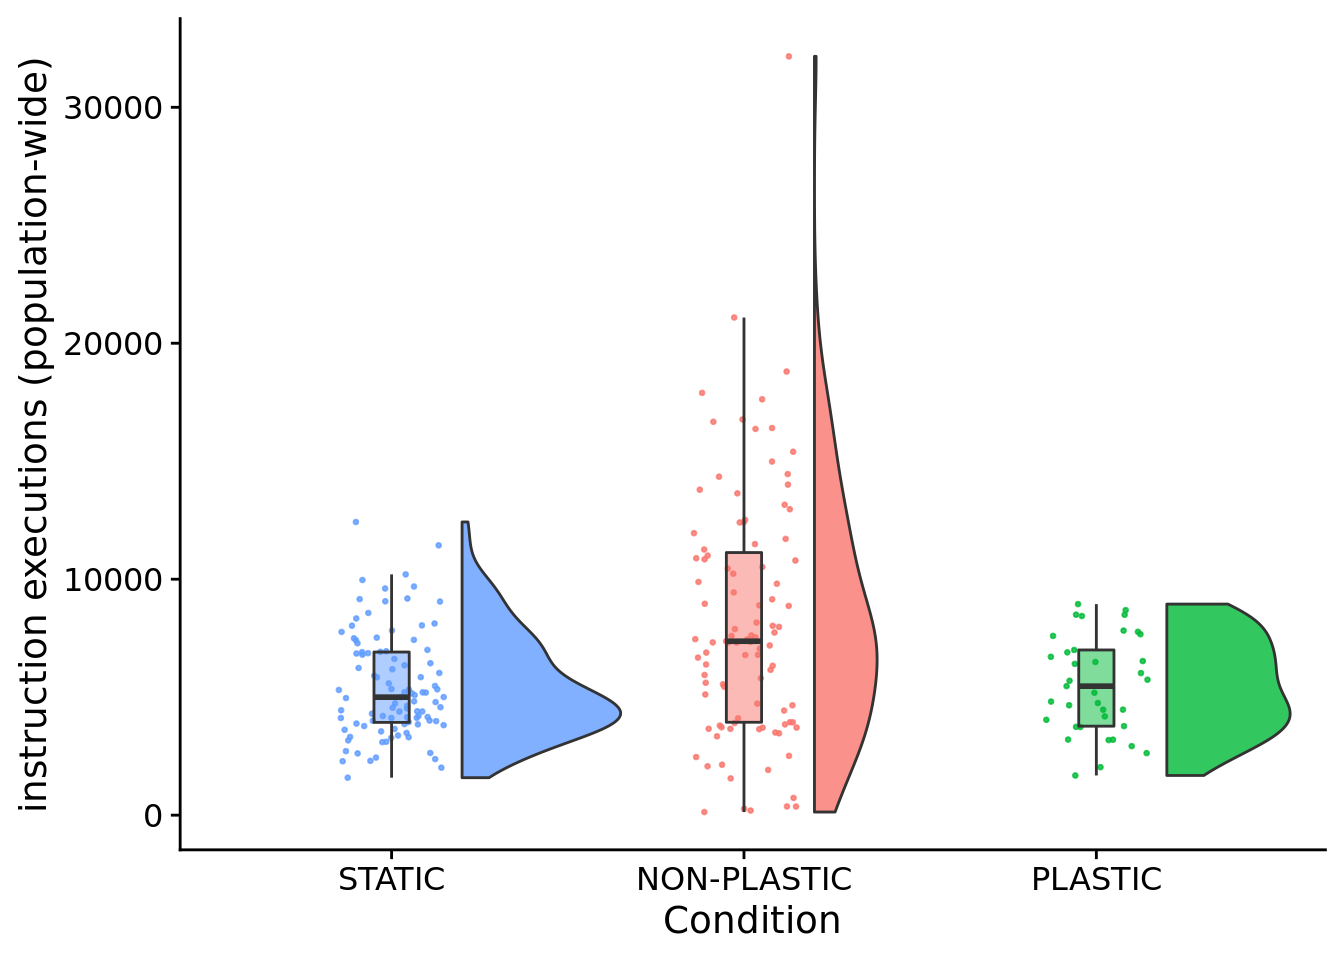
\includegraphics{supplemental-material_files/figure-latex/unnamed-chunk-58-1.pdf}

\begin{Shaded}
\begin{Highlighting}[]
\KeywordTok{kruskal.test}\NormalTok{(}
  \DataTypeTok{formula=}\NormalTok{dominant_lineage_extra_traits_discovered_per_generation}\OperatorTok{~}\NormalTok{condition,}
  \DataTypeTok{data=}\NormalTok{summary_data}
\NormalTok{)}
\end{Highlighting}
\end{Shaded}

\begin{verbatim}
## 
##  Kruskal-Wallis rank sum test
## 
## data:  dominant_lineage_extra_traits_discovered_per_generation by condition
## Kruskal-Wallis chi-squared = 7.1465, df = 2, p-value = 0.02806
\end{verbatim}

\begin{Shaded}
\begin{Highlighting}[]
\KeywordTok{pairwise.wilcox.test}\NormalTok{(}
  \DataTypeTok{x=}\NormalTok{summary_data}\OperatorTok{$}\NormalTok{dominant_lineage_extra_traits_discovered_per_generation,}
  \DataTypeTok{g=}\NormalTok{summary_data}\OperatorTok{$}\NormalTok{condition,}
  \DataTypeTok{p.adjust.method=}\StringTok{"bonferroni"}\NormalTok{,}
  \DataTypeTok{conf.int=}\OtherTok{TRUE}\NormalTok{,}
  \DataTypeTok{conf.level=}\FloatTok{0.95}
\NormalTok{)}
\end{Highlighting}
\end{Shaded}

\begin{verbatim}
## 
##  Pairwise comparisons using Wilcoxon rank sum test with continuity correction 
## 
## data:  summary_data$dominant_lineage_extra_traits_discovered_per_generation and summary_data$condition 
## 
##         NON-PLASTIC PLASTIC
## PLASTIC 0.092       -      
## STATIC  1.000       0.025  
## 
## P value adjustment method: bonferroni
\end{verbatim}

\begin{Shaded}
\begin{Highlighting}[]
\KeywordTok{paste}\NormalTok{(}
  \DataTypeTok{sep=}\StringTok{"; "}\NormalTok{,}
  \KeywordTok{paste0}\NormalTok{(}
    \StringTok{"PLASTIC median: "}\NormalTok{,}
    \KeywordTok{median}\NormalTok{(}\KeywordTok{filter}\NormalTok{(summary_data, condition}\OperatorTok{==}\StringTok{"PLASTIC"}\NormalTok{)}\OperatorTok{$}\NormalTok{dominant_lineage_extra_traits_discovered_per_generation)}
\NormalTok{  ),}
  \KeywordTok{paste0}\NormalTok{(}
    \StringTok{"STATIC median: "}\NormalTok{,}
    \KeywordTok{median}\NormalTok{(}\KeywordTok{filter}\NormalTok{(summary_data, condition}\OperatorTok{==}\StringTok{"STATIC"}\NormalTok{)}\OperatorTok{$}\NormalTok{dominant_lineage_extra_traits_discovered_per_generation)}
\NormalTok{  ),}
  \KeywordTok{paste0}\NormalTok{(}
    \StringTok{"NON-PLASTIC median: "}\NormalTok{,}
    \KeywordTok{median}\NormalTok{(}\KeywordTok{filter}\NormalTok{(summary_data, condition}\OperatorTok{==}\StringTok{"NON-PLASTIC"}\NormalTok{)}\OperatorTok{$}\NormalTok{dominant_lineage_extra_traits_discovered_per_generation)}
\NormalTok{  )}
\NormalTok{)}
\end{Highlighting}
\end{Shaded}

\begin{verbatim}
## [1] "PLASTIC median: 0.000117695011124939; STATIC median: 0.00015363220504867; NON-PLASTIC median: 0.00014358046266055"
\end{verbatim}

\begin{Shaded}
\begin{Highlighting}[]
\KeywordTok{print}\NormalTok{(}\StringTok{"Wilcox rank sum test statistics:"}\NormalTok{)}
\end{Highlighting}
\end{Shaded}

\begin{verbatim}
## [1] "Wilcox rank sum test statistics:"
\end{verbatim}

\begin{Shaded}
\begin{Highlighting}[]
\ControlFlowTok{for}\NormalTok{ (pair }\ControlFlowTok{in}\NormalTok{ pairwise_comparisons) \{}
\NormalTok{  pair_data <-}\StringTok{ }\KeywordTok{filter}\NormalTok{(summary_data, condition }\OperatorTok\StringTok{ }\NormalTok{pair)}
\NormalTok{  pair_data}\OperatorTok{$}\NormalTok{condition <-}\StringTok{ }\KeywordTok{as.factor}\NormalTok{(pair_data}\OperatorTok{$}\NormalTok{condition)}
\NormalTok{  wt <-}\StringTok{ }\KeywordTok{wilcox.test}\NormalTok{(}
    \DataTypeTok{formula=}\NormalTok{dominant_lineage_extra_traits_discovered_per_generation}\OperatorTok{~}\NormalTok{condition,}
    \DataTypeTok{data=}\NormalTok{pair_data,}
    \DataTypeTok{exact=}\OtherTok{FALSE}\NormalTok{,}
    \DataTypeTok{paired=}\OtherTok{FALSE}
\NormalTok{  )}
  \KeywordTok{print}\NormalTok{(}\KeywordTok{paste0}\NormalTok{(pair[}\DecValTok{1}\NormalTok{], }\StringTok{"<-->"}\NormalTok{, pair[}\DecValTok{2}\NormalTok{], }\StringTok{": W="}\NormalTok{,wt}\OperatorTok{$}\NormalTok{statistic))}
\NormalTok{\}}
\end{Highlighting}
\end{Shaded}

\begin{verbatim}
## [1] "STATIC<-->NON-PLASTIC: W=4751"
## [1] "STATIC<-->PLASTIC: W=1510.5"
## [1] "PLASTIC<-->NON-PLASTIC: W=2584"
\end{verbatim}

\hypertarget{novel-functions-gained-lineage}{%
\section{Novel functions gained (lineage)}\label{novel-functions-gained-lineage}}

\begin{Shaded}
\begin{Highlighting}[]
\KeywordTok{ggplot}\NormalTok{(}
\NormalTok{    summary_data,}
    \KeywordTok{aes}\NormalTok{(}\DataTypeTok{x=}\NormalTok{condition, }\DataTypeTok{y=}\NormalTok{dominant_lineage_extra_traits_gained, }\DataTypeTok{fill=}\NormalTok{condition)}
\NormalTok{  ) }\OperatorTok{+}
\StringTok{  }\KeywordTok{geom_flat_violin}\NormalTok{(}
    \DataTypeTok{position =} \KeywordTok{position_nudge}\NormalTok{(}\DataTypeTok{x =} \FloatTok{.2}\NormalTok{, }\DataTypeTok{y =} \DecValTok{0}\NormalTok{),}
    \DataTypeTok{alpha =} \FloatTok{.8}
\NormalTok{  ) }\OperatorTok{+}
\StringTok{  }\KeywordTok{geom_point}\NormalTok{(}
    \DataTypeTok{mapping=}\KeywordTok{aes}\NormalTok{(}\DataTypeTok{color=}\NormalTok{condition),}
    \DataTypeTok{position =} \KeywordTok{position_jitter}\NormalTok{(}\DataTypeTok{width =} \FloatTok{.15}\NormalTok{),}
    \DataTypeTok{size =} \FloatTok{.5}\NormalTok{,}
    \DataTypeTok{alpha =} \FloatTok{0.8}
\NormalTok{  ) }\OperatorTok{+}
\StringTok{  }\KeywordTok{geom_boxplot}\NormalTok{(}
    \DataTypeTok{width =} \FloatTok{.1}\NormalTok{,}
    \DataTypeTok{outlier.shape =} \OtherTok{NA}\NormalTok{,}
    \DataTypeTok{alpha =} \FloatTok{0.5}
\NormalTok{  ) }\OperatorTok{+}
\StringTok{  }\KeywordTok{scale_x_discrete}\NormalTok{(}
    \DataTypeTok{name=}\StringTok{"Condition"}\NormalTok{,}
    \DataTypeTok{limits=}\NormalTok{condition_order}
\NormalTok{  ) }\OperatorTok{+}
\StringTok{  }\KeywordTok{ylab}\NormalTok{(}\StringTok{"Novel function gains along lineage"}\NormalTok{) }\OperatorTok{+}
\StringTok{  }\KeywordTok{scale_fill_brewer}\NormalTok{(}
    \DataTypeTok{palette=}\NormalTok{cb_palette}
\NormalTok{  ) }\OperatorTok{+}
\StringTok{  }\KeywordTok{scale_color_brewer}\NormalTok{(}
    \DataTypeTok{palette=}\NormalTok{cb_palette}
\NormalTok{  ) }\OperatorTok{+}
\StringTok{  }\KeywordTok{coord_flip}\NormalTok{() }\OperatorTok{+}
\StringTok{  }\KeywordTok{facet_wrap}\NormalTok{(}
    \OperatorTok{~}\NormalTok{extra_task_value,}
    \DataTypeTok{labeller=}\NormalTok{label_both}
\NormalTok{  ) }\OperatorTok{+}
\StringTok{  }\KeywordTok{theme}\NormalTok{(}
    \DataTypeTok{legend.position=}\StringTok{"none"}
\NormalTok{  )}
\end{Highlighting}
\end{Shaded}

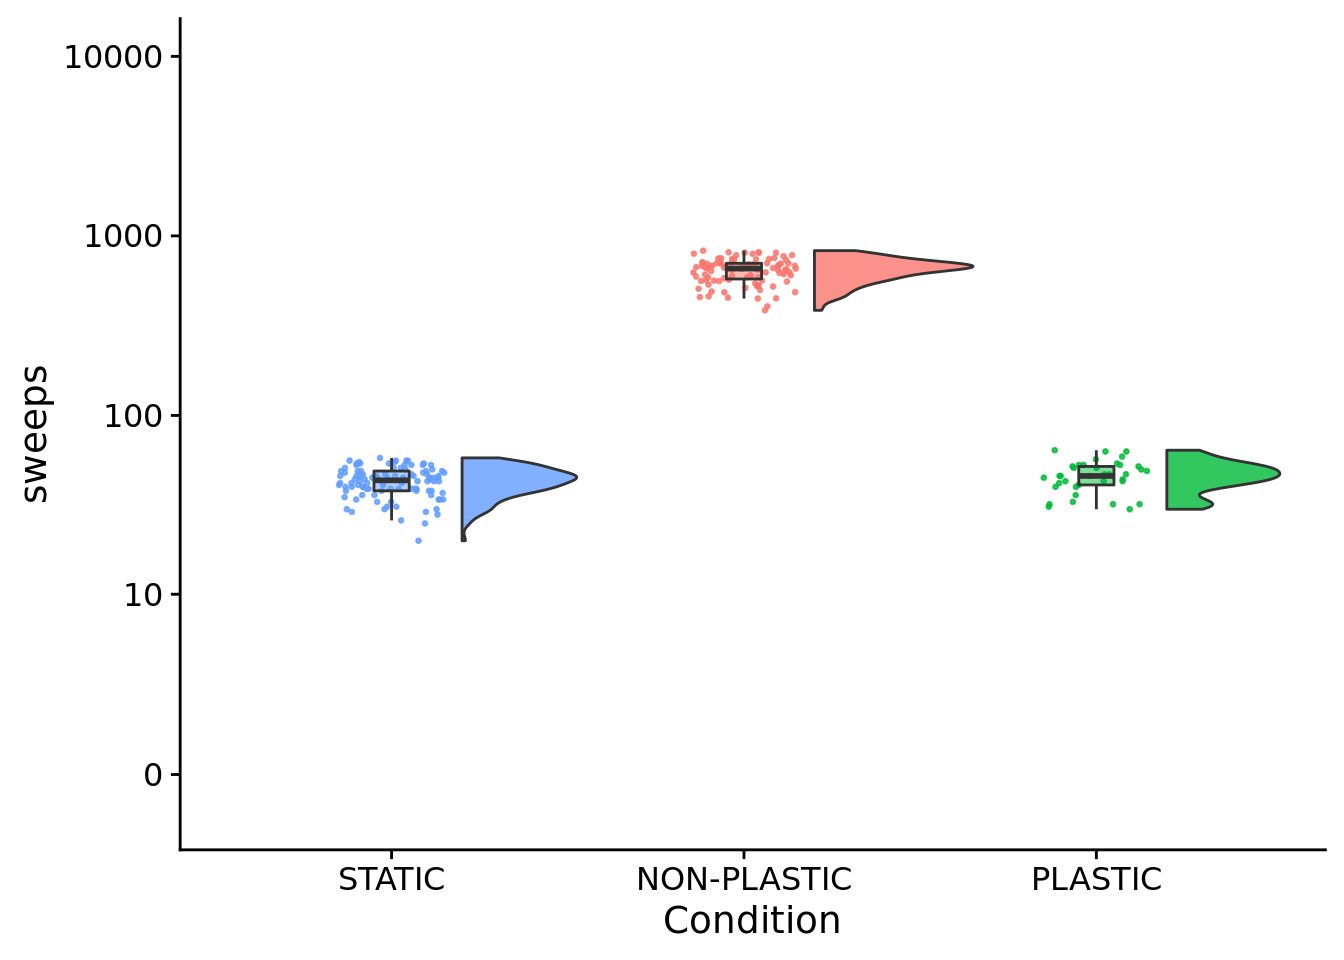
\includegraphics{supplemental-material_files/figure-latex/unnamed-chunk-60-1.pdf}

\begin{Shaded}
\begin{Highlighting}[]
\KeywordTok{ggsave}\NormalTok{(}
  \KeywordTok{paste0}\NormalTok{(working_directory, }\StringTok{"plots/dominant-lineage-extra-tasks-gained.pdf"}\NormalTok{),}
  \DataTypeTok{width=}\DecValTok{15}\NormalTok{,}
  \DataTypeTok{height=}\DecValTok{10}
\NormalTok{)}
\end{Highlighting}
\end{Shaded}

\hypertarget{novel-function-loss-lineage}{%
\section{Novel function loss (lineage)}\label{novel-function-loss-lineage}}

\begin{Shaded}
\begin{Highlighting}[]
\CommentTok{# Compute manual labels for geom_signif}
\NormalTok{stat.test <-}\StringTok{ }\NormalTok{summary_data }\OperatorTok
\StringTok{  }\KeywordTok{wilcox_test}\NormalTok{(dominant_lineage_extra_traits_lost }\OperatorTok{~}\StringTok{ }\NormalTok{condition) }\OperatorTok
\StringTok{  }\KeywordTok{adjust_pvalue}\NormalTok{(}\DataTypeTok{method =} \StringTok{"bonferroni"}\NormalTok{) }\OperatorTok
\StringTok{  }\KeywordTok{add_significance}\NormalTok{() }\OperatorTok
\StringTok{  }\KeywordTok{add_xy_position}\NormalTok{(}\DataTypeTok{x=}\StringTok{"condition"}\NormalTok{, }\DataTypeTok{step.increase=}\DecValTok{1}\NormalTok{)}
\CommentTok{# Tweak y.position manually to account for scaled axis (edge case that triggers bad behavior in geom_signif)}
\NormalTok{stat.test}\OperatorTok{$}\NormalTok{manual_position <-}\StringTok{  }\KeywordTok{log10}\NormalTok{(stat.test}\OperatorTok{$}\NormalTok{y.position) }\OperatorTok{*}\StringTok{ }\KeywordTok{c}\NormalTok{(}\FloatTok{1.0}\NormalTok{,}\FloatTok{1.0}\NormalTok{,}\FloatTok{1.03}\NormalTok{)}
\NormalTok{stat.test}\OperatorTok{$}\NormalTok{label <-}\StringTok{ }\KeywordTok{mapply}\NormalTok{(p_label,stat.test}\OperatorTok{$}\NormalTok{p.adj)}

\NormalTok{summary_data}\OperatorTok{$}\NormalTok{is_outlier <-}\StringTok{ }\KeywordTok{mapply}\NormalTok{(}
\NormalTok{  is_outlier,}
\NormalTok{  summary_data}\OperatorTok{$}\NormalTok{dominant_lineage_extra_traits_lost,}
\NormalTok{  summary_data}\OperatorTok{$}\NormalTok{condition,}
  \DataTypeTok{MoreArgs=}\KeywordTok{list}\NormalTok{(}\DataTypeTok{data=}\NormalTok{summary_data, }\DataTypeTok{column=}\StringTok{"dominant_lineage_extra_traits_lost"}\NormalTok{)}
\NormalTok{)}

\NormalTok{lineage_novel_task_loss_fig <-}\StringTok{ }\KeywordTok{ggplot}\NormalTok{(}
\NormalTok{    summary_data,}
    \KeywordTok{aes}\NormalTok{(}\DataTypeTok{x=}\NormalTok{condition, }\DataTypeTok{y=}\NormalTok{dominant_lineage_extra_traits_lost, }\DataTypeTok{fill=}\NormalTok{condition)}
\NormalTok{  ) }\OperatorTok{+}
\StringTok{  }\KeywordTok{geom_flat_violin}\NormalTok{(}
    \CommentTok{# data=filter(summary_data,is_outlier==FALSE),}
    \DataTypeTok{scale=}\StringTok{"width"}\NormalTok{,}
    \DataTypeTok{position =} \KeywordTok{position_nudge}\NormalTok{(}\DataTypeTok{x =} \FloatTok{.2}\NormalTok{, }\DataTypeTok{y =} \DecValTok{0}\NormalTok{),}
    \DataTypeTok{alpha =} \FloatTok{.8}
\NormalTok{  ) }\OperatorTok{+}
\StringTok{  }\KeywordTok{geom_point}\NormalTok{(}
    \DataTypeTok{mapping=}\KeywordTok{aes}\NormalTok{(}\DataTypeTok{color=}\NormalTok{condition),}
    \DataTypeTok{position =} \KeywordTok{position_jitter}\NormalTok{(}\DataTypeTok{width =} \FloatTok{.15}\NormalTok{),}
    \DataTypeTok{size =} \FloatTok{.5}\NormalTok{,}
    \DataTypeTok{alpha =} \FloatTok{0.8}
\NormalTok{  ) }\OperatorTok{+}
\StringTok{  }\KeywordTok{geom_boxplot}\NormalTok{(}
    \DataTypeTok{width =} \FloatTok{.1}\NormalTok{,}
    \DataTypeTok{outlier.shape =} \OtherTok{NA}\NormalTok{,}
    \DataTypeTok{alpha =} \FloatTok{0.5}
\NormalTok{  ) }\OperatorTok{+}
\StringTok{  }\KeywordTok{scale_x_discrete}\NormalTok{(}
    \DataTypeTok{name=}\StringTok{"Condition"}\NormalTok{,}
    \DataTypeTok{limits=}\NormalTok{condition_order,}
    \DataTypeTok{labels=}\NormalTok{condition_order}
\NormalTok{  ) }\OperatorTok{+}
\StringTok{  }\KeywordTok{scale_y_continuous}\NormalTok{(}
    \DataTypeTok{name=}\StringTok{"Novel function loss (log scale)"}\NormalTok{,}
    \DataTypeTok{trans=}\KeywordTok{pseudo_log_trans}\NormalTok{(}\DataTypeTok{sigma=}\DecValTok{1}\NormalTok{, }\DataTypeTok{base=}\DecValTok{10}\NormalTok{),}
    \DataTypeTok{breaks=}\KeywordTok{c}\NormalTok{(}\DecValTok{0}\NormalTok{,}\DecValTok{10}\NormalTok{,}\DecValTok{100}\NormalTok{,}\DecValTok{1000}\NormalTok{),}
    \DataTypeTok{limits=}\KeywordTok{c}\NormalTok{(}\OperatorTok{-}\DecValTok{1}\NormalTok{,}\DecValTok{5000}\NormalTok{)}
\NormalTok{  ) }\OperatorTok{+}
\StringTok{  }\KeywordTok{scale_fill_brewer}\NormalTok{(}
    \DataTypeTok{palette=}\NormalTok{cb_palette}
\NormalTok{  ) }\OperatorTok{+}
\StringTok{  }\KeywordTok{scale_color_brewer}\NormalTok{(}
    \DataTypeTok{palette=}\NormalTok{cb_palette}
\NormalTok{  ) }\OperatorTok{+}
\StringTok{  }\KeywordTok{labs}\NormalTok{(}
    \DataTypeTok{subtitle=}\KeywordTok{paste0}\NormalTok{(}
      \StringTok{"Kruskal-Wallis, "}\NormalTok{,}
      \KeywordTok{p_label}\NormalTok{(}\KeywordTok{signif}\NormalTok{(}\KeywordTok{kruskal.test}\NormalTok{(}\DataTypeTok{formula=}\NormalTok{dominant_lineage_extra_traits_lost}\OperatorTok{~}\NormalTok{condition, }\DataTypeTok{data=}\NormalTok{summary_data)}\OperatorTok{$}\NormalTok{p.value,}\DataTypeTok{digits=}\DecValTok{4}\NormalTok{))}
\NormalTok{    )}
\NormalTok{  ) }\OperatorTok{+}
\StringTok{  }\NormalTok{ggsignif}\OperatorTok{::}\KeywordTok{geom_signif}\NormalTok{(}
    \DataTypeTok{data=}\KeywordTok{filter}\NormalTok{(stat.test, p.adj}\OperatorTok{<=}\NormalTok{alpha),}
    \KeywordTok{aes}\NormalTok{(}\DataTypeTok{xmin=}\NormalTok{group1,}\DataTypeTok{xmax=}\NormalTok{group2,}\DataTypeTok{annotations=}\NormalTok{label,}\DataTypeTok{y_position=}\NormalTok{manual_position),}
    \DataTypeTok{manual=}\OtherTok{TRUE}\NormalTok{,}
    \DataTypeTok{inherit.aes=}\OtherTok{FALSE}
\NormalTok{  ) }\OperatorTok{+}
\StringTok{  }\CommentTok{# coord_flip()}
\StringTok{  }\KeywordTok{theme}\NormalTok{(}
    \DataTypeTok{legend.position=}\StringTok{"none"}
\NormalTok{  )}
\end{Highlighting}
\end{Shaded}

\begin{verbatim}
## Warning: Ignoring unknown aesthetics: xmin, xmax, annotations, y_position
\end{verbatim}

\begin{Shaded}
\begin{Highlighting}[]
\NormalTok{lineage_novel_task_loss_fig}
\end{Highlighting}
\end{Shaded}

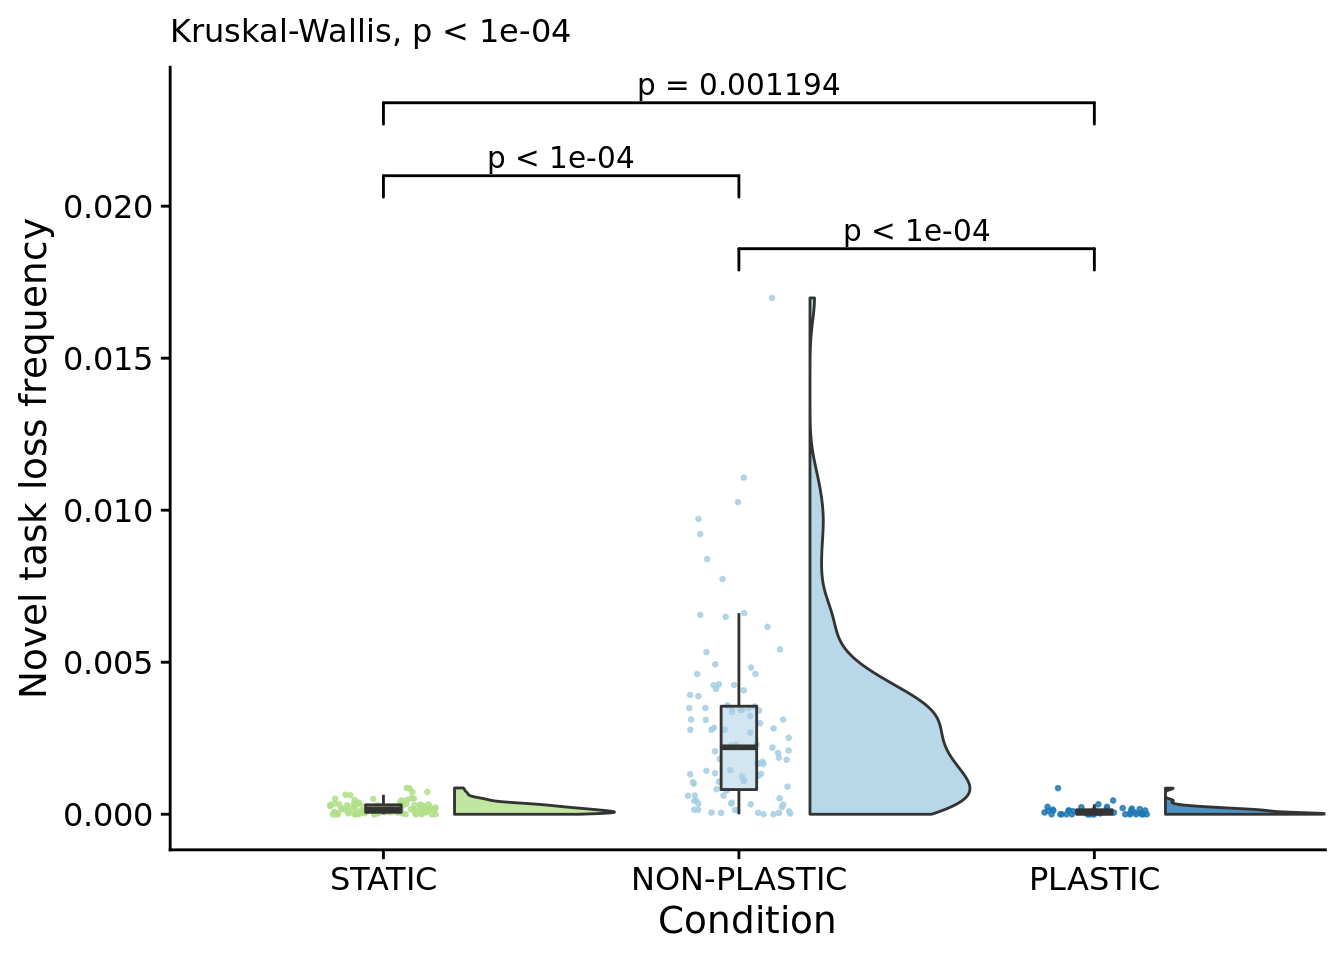
\includegraphics{supplemental-material_files/figure-latex/unnamed-chunk-61-1.pdf}

\begin{Shaded}
\begin{Highlighting}[]
\KeywordTok{kruskal.test}\NormalTok{(}
  \DataTypeTok{formula=}\NormalTok{dominant_lineage_extra_traits_lost}\OperatorTok{~}\NormalTok{condition,}
  \DataTypeTok{data=}\NormalTok{summary_data}
\NormalTok{)}
\end{Highlighting}
\end{Shaded}

\begin{verbatim}
## 
##  Kruskal-Wallis rank sum test
## 
## data:  dominant_lineage_extra_traits_lost by condition
## Kruskal-Wallis chi-squared = 129.06, df = 2, p-value < 2.2e-16
\end{verbatim}

\begin{Shaded}
\begin{Highlighting}[]
\KeywordTok{pairwise.wilcox.test}\NormalTok{(}
  \DataTypeTok{x=}\NormalTok{summary_data}\OperatorTok{$}\NormalTok{dominant_lineage_extra_traits_lost,}
  \DataTypeTok{g=}\NormalTok{summary_data}\OperatorTok{$}\NormalTok{condition,}
  \DataTypeTok{p.adjust.method=}\StringTok{"bonferroni"}\NormalTok{,}
  \DataTypeTok{conf.int=}\OtherTok{TRUE}\NormalTok{,}
  \DataTypeTok{conf.level=}\FloatTok{0.95}
\NormalTok{)}
\end{Highlighting}
\end{Shaded}

\begin{verbatim}
## 
##  Pairwise comparisons using Wilcoxon rank sum test with continuity correction 
## 
## data:  summary_data$dominant_lineage_extra_traits_lost and summary_data$condition 
## 
##         NON-PLASTIC PLASTIC
## PLASTIC 2.7e-16     -      
## STATIC  < 2e-16     0.0024 
## 
## P value adjustment method: bonferroni
\end{verbatim}

\begin{Shaded}
\begin{Highlighting}[]
\KeywordTok{paste}\NormalTok{(}
  \DataTypeTok{sep=}\StringTok{"; "}\NormalTok{,}
  \KeywordTok{paste0}\NormalTok{(}
    \StringTok{"PLASTIC median: "}\NormalTok{,}
    \KeywordTok{median}\NormalTok{(}\KeywordTok{filter}\NormalTok{(summary_data, condition}\OperatorTok{==}\StringTok{"PLASTIC"}\NormalTok{)}\OperatorTok{$}\NormalTok{dominant_lineage_extra_traits_lost)}
\NormalTok{  ),}
  \KeywordTok{paste0}\NormalTok{(}
    \StringTok{"STATIC median: "}\NormalTok{,}
    \KeywordTok{median}\NormalTok{(}\KeywordTok{filter}\NormalTok{(summary_data, condition}\OperatorTok{==}\StringTok{"STATIC"}\NormalTok{)}\OperatorTok{$}\NormalTok{dominant_lineage_extra_traits_lost)}
\NormalTok{  ),}
  \KeywordTok{paste0}\NormalTok{(}
    \StringTok{"NON-PLASTIC median: "}\NormalTok{,}
    \KeywordTok{median}\NormalTok{(}\KeywordTok{filter}\NormalTok{(summary_data, condition}\OperatorTok{==}\StringTok{"NON-PLASTIC"}\NormalTok{)}\OperatorTok{$}\NormalTok{dominant_lineage_extra_traits_lost)}
\NormalTok{  )}
\NormalTok{)}
\end{Highlighting}
\end{Shaded}

\begin{verbatim}
## [1] "PLASTIC median: 2; STATIC median: 5; NON-PLASTIC median: 87.5"
\end{verbatim}

\begin{Shaded}
\begin{Highlighting}[]
\KeywordTok{print}\NormalTok{(}\StringTok{"Wilcox rank sum test statistics:"}\NormalTok{)}
\end{Highlighting}
\end{Shaded}

\begin{verbatim}
## [1] "Wilcox rank sum test statistics:"
\end{verbatim}

\begin{Shaded}
\begin{Highlighting}[]
\ControlFlowTok{for}\NormalTok{ (pair }\ControlFlowTok{in}\NormalTok{ pairwise_comparisons) \{}
\NormalTok{  pair_data <-}\StringTok{ }\KeywordTok{filter}\NormalTok{(summary_data, condition }\OperatorTok\StringTok{ }\NormalTok{pair)}
\NormalTok{  pair_data}\OperatorTok{$}\NormalTok{condition <-}\StringTok{ }\KeywordTok{as.factor}\NormalTok{(pair_data}\OperatorTok{$}\NormalTok{condition)}
\NormalTok{  wt <-}\StringTok{ }\KeywordTok{wilcox.test}\NormalTok{(}
    \DataTypeTok{formula=}\NormalTok{dominant_lineage_extra_traits_lost}\OperatorTok{~}\NormalTok{condition,}
    \DataTypeTok{data=}\NormalTok{pair_data,}
    \DataTypeTok{exact=}\OtherTok{FALSE}\NormalTok{,}
    \DataTypeTok{paired=}\OtherTok{FALSE}
\NormalTok{  )}
  \KeywordTok{print}\NormalTok{(}\KeywordTok{paste0}\NormalTok{(pair[}\DecValTok{1}\NormalTok{], }\StringTok{"<-->"}\NormalTok{, pair[}\DecValTok{2}\NormalTok{], }\StringTok{": W="}\NormalTok{,wt}\OperatorTok{$}\NormalTok{statistic))}
\NormalTok{\}}
\end{Highlighting}
\end{Shaded}

\begin{verbatim}
## [1] "STATIC<-->NON-PLASTIC: W=9105"
## [1] "STATIC<-->PLASTIC: W=1353.5"
## [1] "PLASTIC<-->NON-PLASTIC: W=3959"
\end{verbatim}

\hypertarget{frequency-of-novel-function-loss-lineage}{%
\section{Frequency of novel function loss (lineage)}\label{frequency-of-novel-function-loss-lineage}}

\begin{Shaded}
\begin{Highlighting}[]
\NormalTok{summary_data}\OperatorTok{$}\NormalTok{dominant_lineage_extra_traits_lost_per_generation <-}\StringTok{ }\NormalTok{summary_data}\OperatorTok{$}\NormalTok{dominant_lineage_extra_traits_lost }\OperatorTok{/}\StringTok{ }\NormalTok{summary_data}\OperatorTok{$}\NormalTok{dominant_generation_born}
\NormalTok{summary_data}\OperatorTok{$}\NormalTok{dominant_lineage_extra_traits_generations_per_loss <-}\StringTok{ }\NormalTok{summary_data}\OperatorTok{$}\NormalTok{dominant_generation_born }\OperatorTok{/}\StringTok{ }\NormalTok{summary_data}\OperatorTok{$}\NormalTok{dominant_lineage_extra_traits_lost}

\CommentTok{# Compute manual labels for geom_signif}
\NormalTok{stat.test <-}\StringTok{ }\NormalTok{summary_data }\OperatorTok
\StringTok{  }\KeywordTok{wilcox_test}\NormalTok{(dominant_lineage_extra_traits_lost_per_generation }\OperatorTok{~}\StringTok{ }\NormalTok{condition) }\OperatorTok
\StringTok{  }\KeywordTok{adjust_pvalue}\NormalTok{(}\DataTypeTok{method =} \StringTok{"bonferroni"}\NormalTok{) }\OperatorTok
\StringTok{  }\KeywordTok{add_significance}\NormalTok{() }\OperatorTok
\StringTok{  }\KeywordTok{add_xy_position}\NormalTok{(}\DataTypeTok{x=}\StringTok{"condition"}\NormalTok{, }\DataTypeTok{step.increase=}\NormalTok{.}\DecValTok{1}\NormalTok{)}
\CommentTok{# Tweak y.position manually to account for scaled axis (edge case that triggers bad behavior in geom_signif)}
\NormalTok{stat.test}\OperatorTok{$}\NormalTok{manual_position <-}\StringTok{  }\NormalTok{stat.test}\OperatorTok{$}\NormalTok{y.position }\CommentTok{#* c(1.0,1.0,1.03)}
\NormalTok{stat.test}\OperatorTok{$}\NormalTok{label <-}\StringTok{ }\KeywordTok{mapply}\NormalTok{(p_label,stat.test}\OperatorTok{$}\NormalTok{p.adj)}

\NormalTok{summary_data}\OperatorTok{$}\NormalTok{is_outlier <-}\StringTok{ }\KeywordTok{mapply}\NormalTok{(}
\NormalTok{  is_outlier,}
\NormalTok{  summary_data}\OperatorTok{$}\NormalTok{dominant_lineage_extra_traits_lost_per_generation,}
\NormalTok{  summary_data}\OperatorTok{$}\NormalTok{condition,}
  \DataTypeTok{MoreArgs=}\KeywordTok{list}\NormalTok{(}\DataTypeTok{data=}\NormalTok{summary_data, }\DataTypeTok{column=}\StringTok{"dominant_lineage_extra_traits_lost_per_generation"}\NormalTok{)}
\NormalTok{)}


\NormalTok{lineage_novel_task_loss_freq_fig <-}\StringTok{ }\KeywordTok{ggplot}\NormalTok{(}
    \CommentTok{# filter(summary_data, dominant_lineage_extra_traits_lost > 0),}
\NormalTok{    summary_data,}
    \KeywordTok{aes}\NormalTok{(}\DataTypeTok{x=}\NormalTok{condition, }\DataTypeTok{y=}\NormalTok{dominant_lineage_extra_traits_lost_per_generation, }\DataTypeTok{fill=}\NormalTok{condition)}
\NormalTok{  ) }\OperatorTok{+}
\StringTok{  }\KeywordTok{geom_flat_violin}\NormalTok{(}
    \CommentTok{# data=filter(summary_data,is_outlier==FALSE),}
    \DataTypeTok{scale=}\StringTok{"width"}\NormalTok{,}
    \DataTypeTok{position =} \KeywordTok{position_nudge}\NormalTok{(}\DataTypeTok{x =} \FloatTok{.2}\NormalTok{, }\DataTypeTok{y =} \DecValTok{0}\NormalTok{),}
    \DataTypeTok{alpha =} \FloatTok{.8}
\NormalTok{  ) }\OperatorTok{+}
\StringTok{  }\KeywordTok{geom_point}\NormalTok{(}
    \DataTypeTok{mapping=}\KeywordTok{aes}\NormalTok{(}\DataTypeTok{color=}\NormalTok{condition),}
    \DataTypeTok{position =} \KeywordTok{position_jitter}\NormalTok{(}\DataTypeTok{width =} \FloatTok{.15}\NormalTok{),}
    \DataTypeTok{size =} \FloatTok{.5}\NormalTok{,}
    \DataTypeTok{alpha =} \FloatTok{0.8}
\NormalTok{  ) }\OperatorTok{+}
\StringTok{  }\KeywordTok{geom_boxplot}\NormalTok{(}
    \DataTypeTok{width =} \FloatTok{.1}\NormalTok{,}
    \DataTypeTok{outlier.shape =} \OtherTok{NA}\NormalTok{,}
    \DataTypeTok{alpha =} \FloatTok{0.5}
\NormalTok{  ) }\OperatorTok{+}
\StringTok{  }\KeywordTok{scale_x_discrete}\NormalTok{(}
    \DataTypeTok{name=}\StringTok{"Condition"}\NormalTok{,}
    \DataTypeTok{limits=}\NormalTok{condition_order}
\NormalTok{  ) }\OperatorTok{+}
\StringTok{  }\KeywordTok{ylab}\NormalTok{(}\StringTok{"Novel function loss frequency"}\NormalTok{) }\OperatorTok{+}
\StringTok{  }\KeywordTok{scale_fill_brewer}\NormalTok{(}
    \DataTypeTok{palette=}\NormalTok{cb_palette}
\NormalTok{  ) }\OperatorTok{+}
\StringTok{  }\KeywordTok{scale_color_brewer}\NormalTok{(}
    \DataTypeTok{palette=}\NormalTok{cb_palette}
\NormalTok{  ) }\OperatorTok{+}
\StringTok{  }\KeywordTok{labs}\NormalTok{(}
    \DataTypeTok{subtitle=}\KeywordTok{paste0}\NormalTok{(}
      \StringTok{"Kruskal-Wallis, "}\NormalTok{,}
      \KeywordTok{p_label}\NormalTok{(}\KeywordTok{signif}\NormalTok{(}\KeywordTok{kruskal.test}\NormalTok{(}\DataTypeTok{formula=}\NormalTok{dominant_lineage_extra_traits_lost_per_generation}\OperatorTok{~}\NormalTok{condition, }\DataTypeTok{data=}\NormalTok{summary_data)}\OperatorTok{$}\NormalTok{p.value,}\DataTypeTok{digits=}\DecValTok{4}\NormalTok{))}
\NormalTok{    )}
\NormalTok{  ) }\OperatorTok{+}
\StringTok{  }\NormalTok{ggsignif}\OperatorTok{::}\KeywordTok{geom_signif}\NormalTok{(}
    \DataTypeTok{data=}\KeywordTok{filter}\NormalTok{(stat.test, p.adj}\OperatorTok{<=}\NormalTok{alpha),}
    \KeywordTok{aes}\NormalTok{(}\DataTypeTok{xmin=}\NormalTok{group1,}\DataTypeTok{xmax=}\NormalTok{group2,}\DataTypeTok{annotations=}\NormalTok{label,}\DataTypeTok{y_position=}\NormalTok{manual_position),}
    \DataTypeTok{manual=}\OtherTok{TRUE}\NormalTok{,}
    \DataTypeTok{inherit.aes=}\OtherTok{FALSE}
\NormalTok{  ) }\OperatorTok{+}
\StringTok{  }\KeywordTok{theme}\NormalTok{(}
    \DataTypeTok{legend.position=}\StringTok{"none"}
\NormalTok{  )}
\end{Highlighting}
\end{Shaded}

\begin{verbatim}
## Warning: Ignoring unknown aesthetics: xmin, xmax, annotations, y_position
\end{verbatim}

\begin{Shaded}
\begin{Highlighting}[]
\NormalTok{lineage_novel_task_loss_freq_fig}
\end{Highlighting}
\end{Shaded}

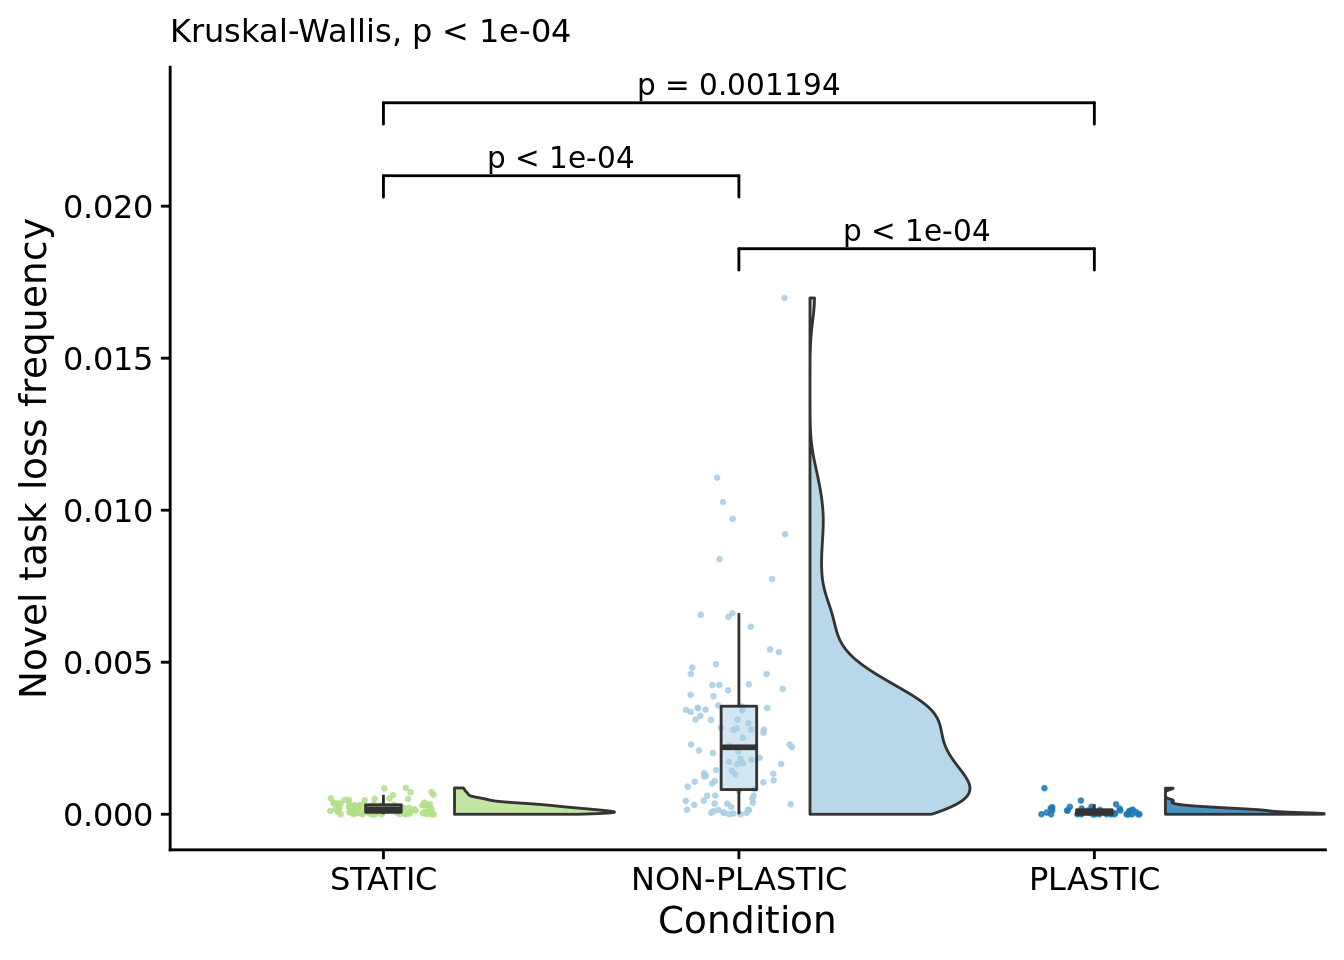
\includegraphics{supplemental-material_files/figure-latex/unnamed-chunk-63-1.pdf}

\begin{Shaded}
\begin{Highlighting}[]
\KeywordTok{kruskal.test}\NormalTok{(}
  \DataTypeTok{formula=}\NormalTok{dominant_lineage_extra_traits_lost_per_generation}\OperatorTok{~}\NormalTok{condition,}
  \DataTypeTok{data=}\NormalTok{summary_data}
\NormalTok{)}
\end{Highlighting}
\end{Shaded}

\begin{verbatim}
## 
##  Kruskal-Wallis rank sum test
## 
## data:  dominant_lineage_extra_traits_lost_per_generation by condition
## Kruskal-Wallis chi-squared = 121.41, df = 2, p-value < 2.2e-16
\end{verbatim}

\begin{Shaded}
\begin{Highlighting}[]
\KeywordTok{pairwise.wilcox.test}\NormalTok{(}
  \DataTypeTok{x=}\NormalTok{summary_data}\OperatorTok{$}\NormalTok{dominant_lineage_extra_traits_lost_per_generation,}
  \DataTypeTok{g=}\NormalTok{summary_data}\OperatorTok{$}\NormalTok{condition,}
  \DataTypeTok{p.adjust.method=}\StringTok{"bonferroni"}\NormalTok{,}
  \DataTypeTok{conf.int=}\OtherTok{TRUE}\NormalTok{,}
  \DataTypeTok{conf.level=}\FloatTok{0.95}
\NormalTok{)}
\end{Highlighting}
\end{Shaded}

\begin{verbatim}
## 
##  Pairwise comparisons using Wilcoxon rank sum test with continuity correction 
## 
## data:  summary_data$dominant_lineage_extra_traits_lost_per_generation and summary_data$condition 
## 
##         NON-PLASTIC PLASTIC
## PLASTIC 1.1e-15     -      
## STATIC  < 2e-16     0.0012 
## 
## P value adjustment method: bonferroni
\end{verbatim}

\begin{Shaded}
\begin{Highlighting}[]
\KeywordTok{paste}\NormalTok{(}
  \DataTypeTok{sep=}\StringTok{"; "}\NormalTok{,}
  \KeywordTok{paste0}\NormalTok{(}
    \StringTok{"PLASTIC median: "}\NormalTok{,}
    \KeywordTok{median}\NormalTok{(}\KeywordTok{filter}\NormalTok{(summary_data, condition}\OperatorTok{==}\StringTok{"PLASTIC"}\NormalTok{)}\OperatorTok{$}\NormalTok{dominant_lineage_extra_traits_lost_per_generation)}
\NormalTok{  ),}
  \KeywordTok{paste0}\NormalTok{(}
    \StringTok{"STATIC median: "}\NormalTok{,}
    \KeywordTok{median}\NormalTok{(}\KeywordTok{filter}\NormalTok{(summary_data, condition}\OperatorTok{==}\StringTok{"STATIC"}\NormalTok{)}\OperatorTok{$}\NormalTok{dominant_lineage_extra_traits_lost_per_generation)}
\NormalTok{  ),}
  \KeywordTok{paste0}\NormalTok{(}
    \StringTok{"NON-PLASTIC median: "}\NormalTok{,}
    \KeywordTok{median}\NormalTok{(}\KeywordTok{filter}\NormalTok{(summary_data, condition}\OperatorTok{==}\StringTok{"NON-PLASTIC"}\NormalTok{)}\OperatorTok{$}\NormalTok{dominant_lineage_extra_traits_lost_per_generation)}
\NormalTok{  )}
\NormalTok{)}
\end{Highlighting}
\end{Shaded}

\begin{verbatim}
## [1] "PLASTIC median: 6.25141973661864e-05; STATIC median: 0.000161396283669756; NON-PLASTIC median: 0.0022026054610079"
\end{verbatim}

\begin{Shaded}
\begin{Highlighting}[]
\KeywordTok{print}\NormalTok{(}\StringTok{"Wilcox rank sum test statistics:"}\NormalTok{)}
\end{Highlighting}
\end{Shaded}

\begin{verbatim}
## [1] "Wilcox rank sum test statistics:"
\end{verbatim}

\begin{Shaded}
\begin{Highlighting}[]
\ControlFlowTok{for}\NormalTok{ (pair }\ControlFlowTok{in}\NormalTok{ pairwise_comparisons) \{}
\NormalTok{  pair_data <-}\StringTok{ }\KeywordTok{filter}\NormalTok{(summary_data, condition }\OperatorTok\StringTok{ }\NormalTok{pair)}
\NormalTok{  pair_data}\OperatorTok{$}\NormalTok{condition <-}\StringTok{ }\KeywordTok{as.factor}\NormalTok{(pair_data}\OperatorTok{$}\NormalTok{condition)}
\NormalTok{  wt <-}\StringTok{ }\KeywordTok{wilcox.test}\NormalTok{(}
    \DataTypeTok{formula=}\NormalTok{dominant_lineage_extra_traits_lost_per_generation}\OperatorTok{~}\NormalTok{condition,}
    \DataTypeTok{data=}\NormalTok{pair_data,}
    \DataTypeTok{exact=}\OtherTok{FALSE}\NormalTok{,}
    \DataTypeTok{paired=}\OtherTok{FALSE}
\NormalTok{  )}
  \KeywordTok{print}\NormalTok{(}\KeywordTok{paste0}\NormalTok{(pair[}\DecValTok{1}\NormalTok{], }\StringTok{"<-->"}\NormalTok{, pair[}\DecValTok{2}\NormalTok{], }\StringTok{": W="}\NormalTok{,wt}\OperatorTok{$}\NormalTok{statistic))}
\NormalTok{\}}
\end{Highlighting}
\end{Shaded}

\begin{verbatim}
## [1] "STATIC<-->NON-PLASTIC: W=8940"
## [1] "STATIC<-->PLASTIC: W=1311"
## [1] "PLASTIC<-->NON-PLASTIC: W=3922"
\end{verbatim}

\hypertarget{how-many-instances-of-novel-function-loss-co-occurred-with-changes-in-base-phenotype}{%
\section{How many instances of novel function loss co-occurred with changes in base phenotype?}\label{how-many-instances-of-novel-function-loss-co-occurred-with-changes-in-base-phenotype}}

Function loss linked with base function changes.

\begin{Shaded}
\begin{Highlighting}[]
\NormalTok{lost_traits_summary_data <-}\StringTok{ }\KeywordTok{filter}\NormalTok{(summary_data, extra_task_value}\OperatorTok{==}\FloatTok{0.1} \OperatorTok{&}\StringTok{ }\NormalTok{dominant_lineage_extra_traits_lost}\OperatorTok{>}\DecValTok{0}\NormalTok{)}
\NormalTok{lost_traits_summary_data}\OperatorTok{$}\NormalTok{frac_linked_extra_trait_loss <-}\StringTok{ }\NormalTok{lost_traits_summary_data}\OperatorTok{$}\NormalTok{dominant_lineage_extra_traits_lost_linked_to_primary_change }\OperatorTok{/}\StringTok{ }\NormalTok{lost_traits_summary_data}\OperatorTok{$}\NormalTok{dominant_lineage_extra_traits_lost}
\end{Highlighting}
\end{Shaded}

\begin{Shaded}
\begin{Highlighting}[]
\KeywordTok{ggplot}\NormalTok{(lost_traits_summary_data, }\KeywordTok{aes}\NormalTok{(}\DataTypeTok{x=}\NormalTok{condition, }\DataTypeTok{y=}\NormalTok{frac_linked_extra_trait_loss, }\DataTypeTok{fill=}\NormalTok{condition)) }\OperatorTok{+}
\StringTok{  }\KeywordTok{geom_flat_violin}\NormalTok{(}
    \DataTypeTok{position =} \KeywordTok{position_nudge}\NormalTok{(}\DataTypeTok{x =} \FloatTok{.2}\NormalTok{, }\DataTypeTok{y =} \DecValTok{0}\NormalTok{),}
    \DataTypeTok{alpha =} \FloatTok{.8}
\NormalTok{  ) }\OperatorTok{+}
\StringTok{  }\KeywordTok{geom_point}\NormalTok{(}
    \DataTypeTok{mapping=}\KeywordTok{aes}\NormalTok{(}\DataTypeTok{color=}\NormalTok{condition),}
    \DataTypeTok{position =} \KeywordTok{position_jitter}\NormalTok{(}\DataTypeTok{width =} \FloatTok{.15}\NormalTok{),}
    \DataTypeTok{size =} \FloatTok{.5}\NormalTok{,}
    \DataTypeTok{alpha =} \FloatTok{0.8}
\NormalTok{  ) }\OperatorTok{+}
\StringTok{  }\KeywordTok{geom_boxplot}\NormalTok{(}
    \DataTypeTok{width =} \FloatTok{.1}\NormalTok{,}
    \DataTypeTok{outlier.shape =} \OtherTok{NA}\NormalTok{,}
    \DataTypeTok{alpha =} \FloatTok{0.5}
\NormalTok{  ) }\OperatorTok{+}
\StringTok{  }\KeywordTok{scale_x_discrete}\NormalTok{(}
    \DataTypeTok{name=}\StringTok{"Condition"}\NormalTok{,}
    \DataTypeTok{limits=}\NormalTok{condition_order}
\NormalTok{  ) }\OperatorTok{+}
\StringTok{  }\KeywordTok{scale_fill_brewer}\NormalTok{(}
    \DataTypeTok{palette=}\NormalTok{cb_palette}
\NormalTok{  ) }\OperatorTok{+}
\StringTok{  }\KeywordTok{scale_color_brewer}\NormalTok{(}
    \DataTypeTok{palette=}\NormalTok{cb_palette}
\NormalTok{  ) }\OperatorTok{+}
\StringTok{  }\KeywordTok{theme}\NormalTok{(}
    \DataTypeTok{legend.position=}\StringTok{"none"}
\NormalTok{  )}
\end{Highlighting}
\end{Shaded}

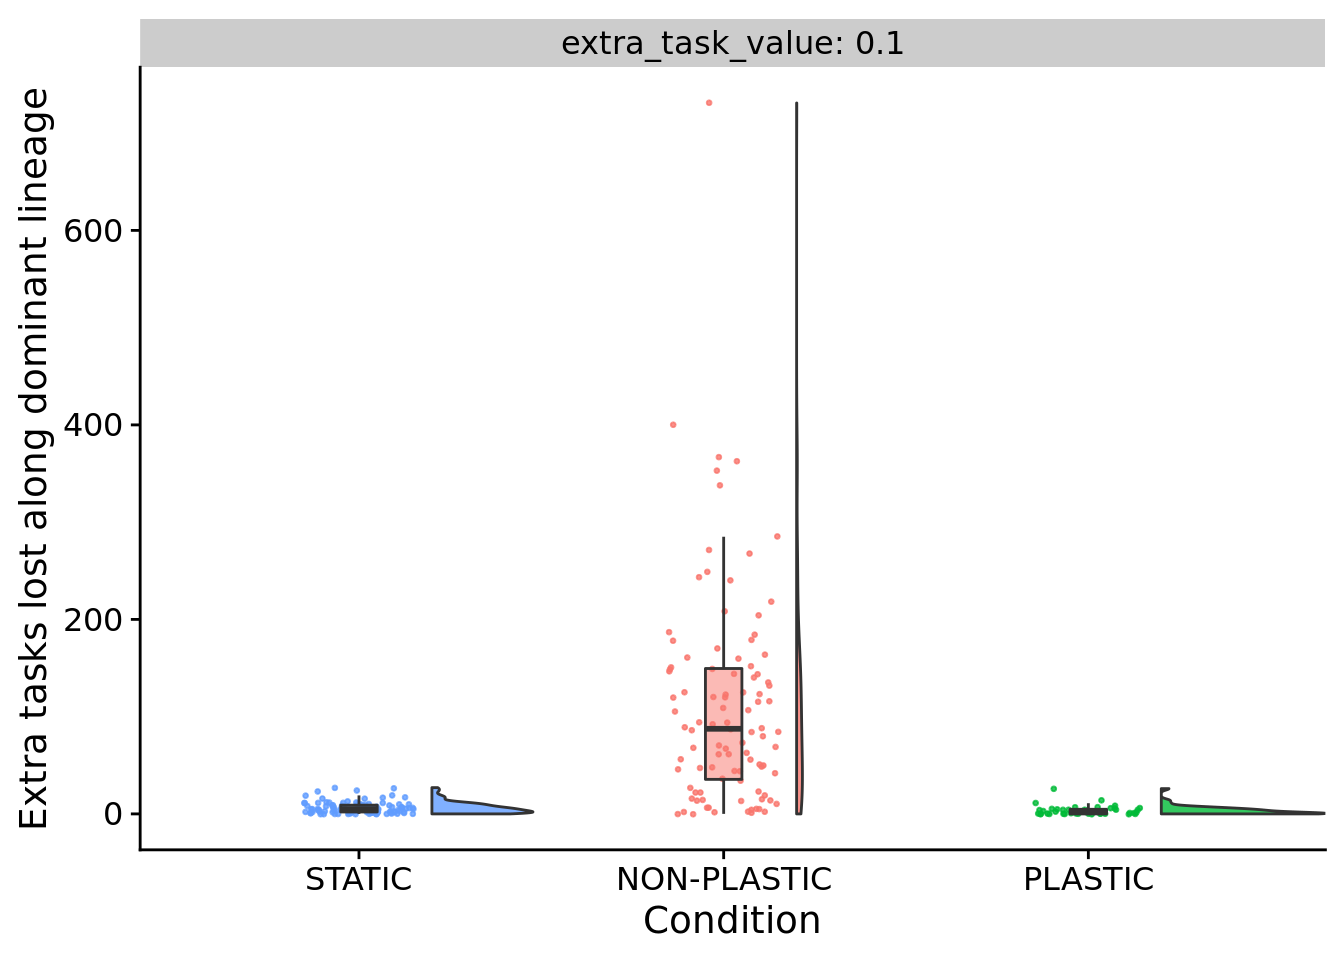
\includegraphics{supplemental-material_files/figure-latex/unnamed-chunk-66-1.pdf}

\begin{Shaded}
\begin{Highlighting}[]
\KeywordTok{kruskal.test}\NormalTok{(}
  \DataTypeTok{formula=}\NormalTok{frac_linked_extra_trait_loss}\OperatorTok{~}\NormalTok{condition,}
  \DataTypeTok{data=}\NormalTok{lost_traits_summary_data}
\NormalTok{)}
\end{Highlighting}
\end{Shaded}

\begin{verbatim}
## 
##  Kruskal-Wallis rank sum test
## 
## data:  frac_linked_extra_trait_loss by condition
## Kruskal-Wallis chi-squared = 153.68, df = 2, p-value < 2.2e-16
\end{verbatim}

\begin{Shaded}
\begin{Highlighting}[]
\KeywordTok{pairwise.wilcox.test}\NormalTok{(}
  \DataTypeTok{x=}\NormalTok{lost_traits_summary_data}\OperatorTok{$}\NormalTok{frac_linked_extra_trait_loss,}
  \DataTypeTok{g=}\NormalTok{lost_traits_summary_data}\OperatorTok{$}\NormalTok{condition,}
  \DataTypeTok{p.adjust.method=}\StringTok{"bonferroni"}\NormalTok{,}
  \DataTypeTok{conf.int=}\OtherTok{TRUE}\NormalTok{,}
  \DataTypeTok{conf.level=}\FloatTok{0.95}
\NormalTok{)}
\end{Highlighting}
\end{Shaded}

\begin{verbatim}
## 
##  Pairwise comparisons using Wilcoxon rank sum test with continuity correction 
## 
## data:  lost_traits_summary_data$frac_linked_extra_trait_loss and lost_traits_summary_data$condition 
## 
##         NON-PLASTIC PLASTIC
## PLASTIC 1.9e-08     -      
## STATIC  < 2e-16     1.8e-06
## 
## P value adjustment method: bonferroni
\end{verbatim}

\begin{Shaded}
\begin{Highlighting}[]
\KeywordTok{paste}\NormalTok{(}
  \DataTypeTok{sep=}\StringTok{"; "}\NormalTok{,}
  \KeywordTok{paste0}\NormalTok{(}
    \StringTok{"PLASTIC median: "}\NormalTok{,}
    \KeywordTok{median}\NormalTok{(}\KeywordTok{filter}\NormalTok{(lost_traits_summary_data, condition}\OperatorTok{==}\StringTok{"PLASTIC"}\NormalTok{)}\OperatorTok{$}\NormalTok{frac_linked_extra_trait_loss)}
\NormalTok{  ),}
  \KeywordTok{paste0}\NormalTok{(}
    \StringTok{"STATIC median: "}\NormalTok{,}
    \KeywordTok{median}\NormalTok{(}\KeywordTok{filter}\NormalTok{(lost_traits_summary_data, condition}\OperatorTok{==}\StringTok{"STATIC"}\NormalTok{)}\OperatorTok{$}\NormalTok{frac_linked_extra_trait_loss)}
\NormalTok{  ),}
  \KeywordTok{paste0}\NormalTok{(}
    \StringTok{"NON-PLASTIC median: "}\NormalTok{,}
    \KeywordTok{median}\NormalTok{(}\KeywordTok{filter}\NormalTok{(lost_traits_summary_data, condition}\OperatorTok{==}\StringTok{"NON-PLASTIC"}\NormalTok{)}\OperatorTok{$}\NormalTok{frac_linked_extra_trait_loss)}
\NormalTok{  )}
\NormalTok{)}
\end{Highlighting}
\end{Shaded}

\begin{verbatim}
## [1] "PLASTIC median: 0.0192307692307692; STATIC median: 0; NON-PLASTIC median: 0.983803278688525"
\end{verbatim}

\begin{Shaded}
\begin{Highlighting}[]
\KeywordTok{print}\NormalTok{(}\StringTok{"Wilcox rank sum test statistics:"}\NormalTok{)}
\end{Highlighting}
\end{Shaded}

\begin{verbatim}
## [1] "Wilcox rank sum test statistics:"
\end{verbatim}

\begin{Shaded}
\begin{Highlighting}[]
\ControlFlowTok{for}\NormalTok{ (pair }\ControlFlowTok{in}\NormalTok{ pairwise_comparisons) \{}
\NormalTok{  pair_data <-}\StringTok{ }\KeywordTok{filter}\NormalTok{(lost_traits_summary_data, condition }\OperatorTok\StringTok{ }\NormalTok{pair)}
\NormalTok{  pair_data}\OperatorTok{$}\NormalTok{condition <-}\StringTok{ }\KeywordTok{as.factor}\NormalTok{(pair_data}\OperatorTok{$}\NormalTok{condition)}
\NormalTok{  wt <-}\StringTok{ }\KeywordTok{wilcox.test}\NormalTok{(}
    \DataTypeTok{formula=}\NormalTok{frac_linked_extra_trait_loss}\OperatorTok{~}\NormalTok{condition,}
    \DataTypeTok{data=}\NormalTok{pair_data,}
    \DataTypeTok{exact=}\OtherTok{FALSE}\NormalTok{,}
    \DataTypeTok{paired=}\OtherTok{FALSE}
\NormalTok{  )}
  \KeywordTok{print}\NormalTok{(}\KeywordTok{paste0}\NormalTok{(pair[}\DecValTok{1}\NormalTok{], }\StringTok{"<-->"}\NormalTok{, pair[}\DecValTok{2}\NormalTok{], }\StringTok{": W="}\NormalTok{,wt}\OperatorTok{$}\NormalTok{statistic))}
\NormalTok{\}}
\end{Highlighting}
\end{Shaded}

\begin{verbatim}
## [1] "STATIC<-->NON-PLASTIC: W=8344"
## [1] "STATIC<-->PLASTIC: W=1602"
## [1] "PLASTIC<-->NON-PLASTIC: W=2212"
\end{verbatim}

\begin{Shaded}
\begin{Highlighting}[]
\KeywordTok{sum}\NormalTok{(}\KeywordTok{filter}\NormalTok{(lost_traits_summary_data, condition}\OperatorTok{==}\StringTok{"NON-PLASTIC"}\NormalTok{)}\OperatorTok{$}\NormalTok{dominant_lineage_extra_traits_lost_linked_to_primary_change)}
\end{Highlighting}
\end{Shaded}

\begin{verbatim}
## [1] 10998
\end{verbatim}

\begin{Shaded}
\begin{Highlighting}[]
\KeywordTok{sum}\NormalTok{(}\KeywordTok{filter}\NormalTok{(lost_traits_summary_data, condition}\OperatorTok{==}\StringTok{"NON-PLASTIC"}\NormalTok{)}\OperatorTok{$}\NormalTok{dominant_lineage_extra_traits_lost)}
\end{Highlighting}
\end{Shaded}

\begin{verbatim}
## [1] 11229
\end{verbatim}

\begin{Shaded}
\begin{Highlighting}[]
\NormalTok{aggregate_frac_linked_extra_trait_loss_nonplastic <-}\StringTok{ }\KeywordTok{sum}\NormalTok{(}\KeywordTok{filter}\NormalTok{(lost_traits_summary_data, condition}\OperatorTok{==}\StringTok{"NON-PLASTIC"}\NormalTok{)}\OperatorTok{$}\NormalTok{dominant_lineage_extra_traits_lost_linked_to_primary_change) }\OperatorTok{/}\StringTok{ }\KeywordTok{sum}\NormalTok{(}\KeywordTok{filter}\NormalTok{(lost_traits_summary_data, condition}\OperatorTok{==}\StringTok{"NON-PLASTIC"}\NormalTok{)}\OperatorTok{$}\NormalTok{dominant_lineage_extra_traits_lost)}
\NormalTok{aggregate_frac_linked_extra_trait_loss_nonplastic}
\end{Highlighting}
\end{Shaded}

\begin{verbatim}
## [1] 0.9794283
\end{verbatim}

\begin{Shaded}
\begin{Highlighting}[]
\KeywordTok{sum}\NormalTok{(}\KeywordTok{filter}\NormalTok{(lost_traits_summary_data, condition}\OperatorTok{==}\StringTok{"PLASTIC"}\NormalTok{)}\OperatorTok{$}\NormalTok{dominant_lineage_extra_traits_lost_linked_to_primary_change)}
\end{Highlighting}
\end{Shaded}

\begin{verbatim}
## [1] 29
\end{verbatim}

\begin{Shaded}
\begin{Highlighting}[]
\KeywordTok{sum}\NormalTok{(}\KeywordTok{filter}\NormalTok{(lost_traits_summary_data, condition}\OperatorTok{==}\StringTok{"PLASTIC"}\NormalTok{)}\OperatorTok{$}\NormalTok{dominant_lineage_extra_traits_lost)}
\end{Highlighting}
\end{Shaded}

\begin{verbatim}
## [1] 142
\end{verbatim}

\begin{Shaded}
\begin{Highlighting}[]
\NormalTok{aggregate_frac_linked_extra_trait_loss_plastic <-}\StringTok{ }\KeywordTok{sum}\NormalTok{(}\KeywordTok{filter}\NormalTok{(lost_traits_summary_data, condition}\OperatorTok{==}\StringTok{"PLASTIC"}\NormalTok{)}\OperatorTok{$}\NormalTok{dominant_lineage_extra_traits_lost_linked_to_primary_change) }\OperatorTok{/}\StringTok{ }\KeywordTok{sum}\NormalTok{(}\KeywordTok{filter}\NormalTok{(lost_traits_summary_data, condition}\OperatorTok{==}\StringTok{"PLASTIC"}\NormalTok{)}\OperatorTok{$}\NormalTok{dominant_lineage_extra_traits_lost)}
\NormalTok{aggregate_frac_linked_extra_trait_loss_plastic}
\end{Highlighting}
\end{Shaded}

\begin{verbatim}
## [1] 0.2042254
\end{verbatim}

\begin{Shaded}
\begin{Highlighting}[]
\KeywordTok{sum}\NormalTok{(}\KeywordTok{filter}\NormalTok{(lost_traits_summary_data, condition}\OperatorTok{==}\StringTok{"STATIC"}\NormalTok{)}\OperatorTok{$}\NormalTok{dominant_lineage_extra_traits_lost_linked_to_primary_change)}
\end{Highlighting}
\end{Shaded}

\begin{verbatim}
## [1] 13
\end{verbatim}

\begin{Shaded}
\begin{Highlighting}[]
\KeywordTok{sum}\NormalTok{(}\KeywordTok{filter}\NormalTok{(lost_traits_summary_data, condition}\OperatorTok{==}\StringTok{"STATIC"}\NormalTok{)}\OperatorTok{$}\NormalTok{dominant_lineage_extra_traits_lost)}
\end{Highlighting}
\end{Shaded}

\begin{verbatim}
## [1] 631
\end{verbatim}

\begin{Shaded}
\begin{Highlighting}[]
\NormalTok{aggregate_frac_linked_extra_trait_loss_nonplastic <-}\StringTok{ }\KeywordTok{sum}\NormalTok{(}\KeywordTok{filter}\NormalTok{(lost_traits_summary_data, condition}\OperatorTok{==}\StringTok{"STATIC"}\NormalTok{)}\OperatorTok{$}\NormalTok{dominant_lineage_extra_traits_lost_linked_to_primary_change) }\OperatorTok{/}\StringTok{ }\KeywordTok{sum}\NormalTok{(}\KeywordTok{filter}\NormalTok{(lost_traits_summary_data, condition}\OperatorTok{==}\StringTok{"STATIC"}\NormalTok{)}\OperatorTok{$}\NormalTok{dominant_lineage_extra_traits_lost)}
\NormalTok{aggregate_frac_linked_extra_trait_loss_nonplastic}
\end{Highlighting}
\end{Shaded}

\begin{verbatim}
## [1] 0.02060222
\end{verbatim}

\hypertarget{manuscript-figures-1}{%
\section{Manuscript figures}\label{manuscript-figures-1}}

\hypertarget{combined-panel}{%
\section{Combined panel}\label{combined-panel}}

\begin{Shaded}
\begin{Highlighting}[]
\NormalTok{magnitude_grid <-}\StringTok{ }\KeywordTok{plot_grid}\NormalTok{(}
\NormalTok{  final_novel_task_count_fig }\OperatorTok{+}
\StringTok{    }\KeywordTok{theme}\NormalTok{(}
      \DataTypeTok{axis.title.x=}\KeywordTok{element_blank}\NormalTok{()}
\NormalTok{    ) }\OperatorTok{+}
\StringTok{    }\KeywordTok{ggtitle}\NormalTok{(}\StringTok{"Final novel function count"}\NormalTok{),}
\NormalTok{  lineage_novel_task_discovery_fig }\OperatorTok{+}
\StringTok{    }\KeywordTok{theme}\NormalTok{(}
      \DataTypeTok{axis.title.x=}\KeywordTok{element_blank}\NormalTok{()}
\NormalTok{    ) }\OperatorTok{+}
\StringTok{    }\KeywordTok{ggtitle}\NormalTok{(}\StringTok{"Novel function discovery"}\NormalTok{),}
\NormalTok{  lineage_novel_task_loss_fig }\OperatorTok{+}
\StringTok{    }\KeywordTok{theme}\NormalTok{(}
      \DataTypeTok{axis.title.x=}\KeywordTok{element_blank}\NormalTok{()}
\NormalTok{    ) }\OperatorTok{+}
\StringTok{    }\KeywordTok{ggtitle}\NormalTok{(}\StringTok{"Novel function loss"}\NormalTok{),}
  \DataTypeTok{nrow=}\DecValTok{1}\NormalTok{,}
  \DataTypeTok{align=}\StringTok{"v"}\NormalTok{,}
  \DataTypeTok{labels=}\StringTok{"auto"}
\NormalTok{)}
\NormalTok{magnitude_grid}
\end{Highlighting}
\end{Shaded}

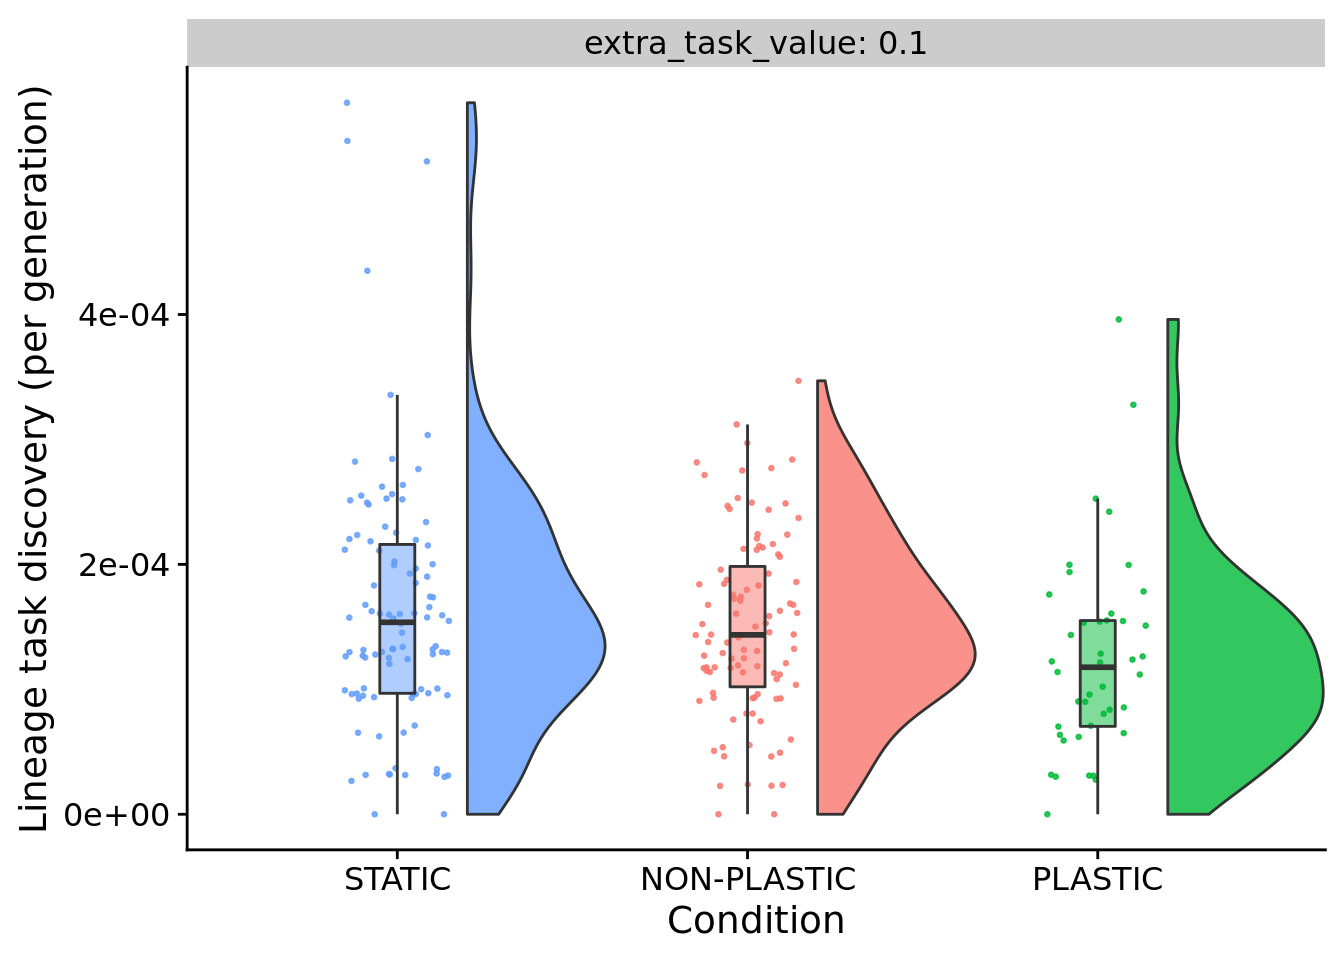
\includegraphics{supplemental-material_files/figure-latex/unnamed-chunk-69-1.pdf}

\begin{Shaded}
\begin{Highlighting}[]
\NormalTok{pace_grid <-}\StringTok{ }\KeywordTok{plot_grid}\NormalTok{(}
\NormalTok{  lineage_novel_task_discovery_freq_fig }\OperatorTok{+}
\StringTok{    }\KeywordTok{theme}\NormalTok{(}
      \DataTypeTok{axis.title.x=}\KeywordTok{element_blank}\NormalTok{()}
\NormalTok{    ) }\OperatorTok{+}
\StringTok{    }\KeywordTok{ggtitle}\NormalTok{(}\StringTok{"Novel function discovery frequency"}\NormalTok{),}
\NormalTok{  lineage_novel_task_loss_freq_fig }\OperatorTok{+}
\StringTok{    }\KeywordTok{theme}\NormalTok{(}
      \DataTypeTok{axis.title.x=}\KeywordTok{element_blank}\NormalTok{()}
\NormalTok{    ) }\OperatorTok{+}
\StringTok{    }\KeywordTok{ggtitle}\NormalTok{(}\StringTok{"Novel function loss frequency"}\NormalTok{),}
  \DataTypeTok{nrow=}\DecValTok{1}\NormalTok{,}
  \DataTypeTok{align=}\StringTok{"v"}\NormalTok{,}
  \DataTypeTok{labels=}\StringTok{"auto"}
\NormalTok{)}
\NormalTok{pace_grid}
\end{Highlighting}
\end{Shaded}

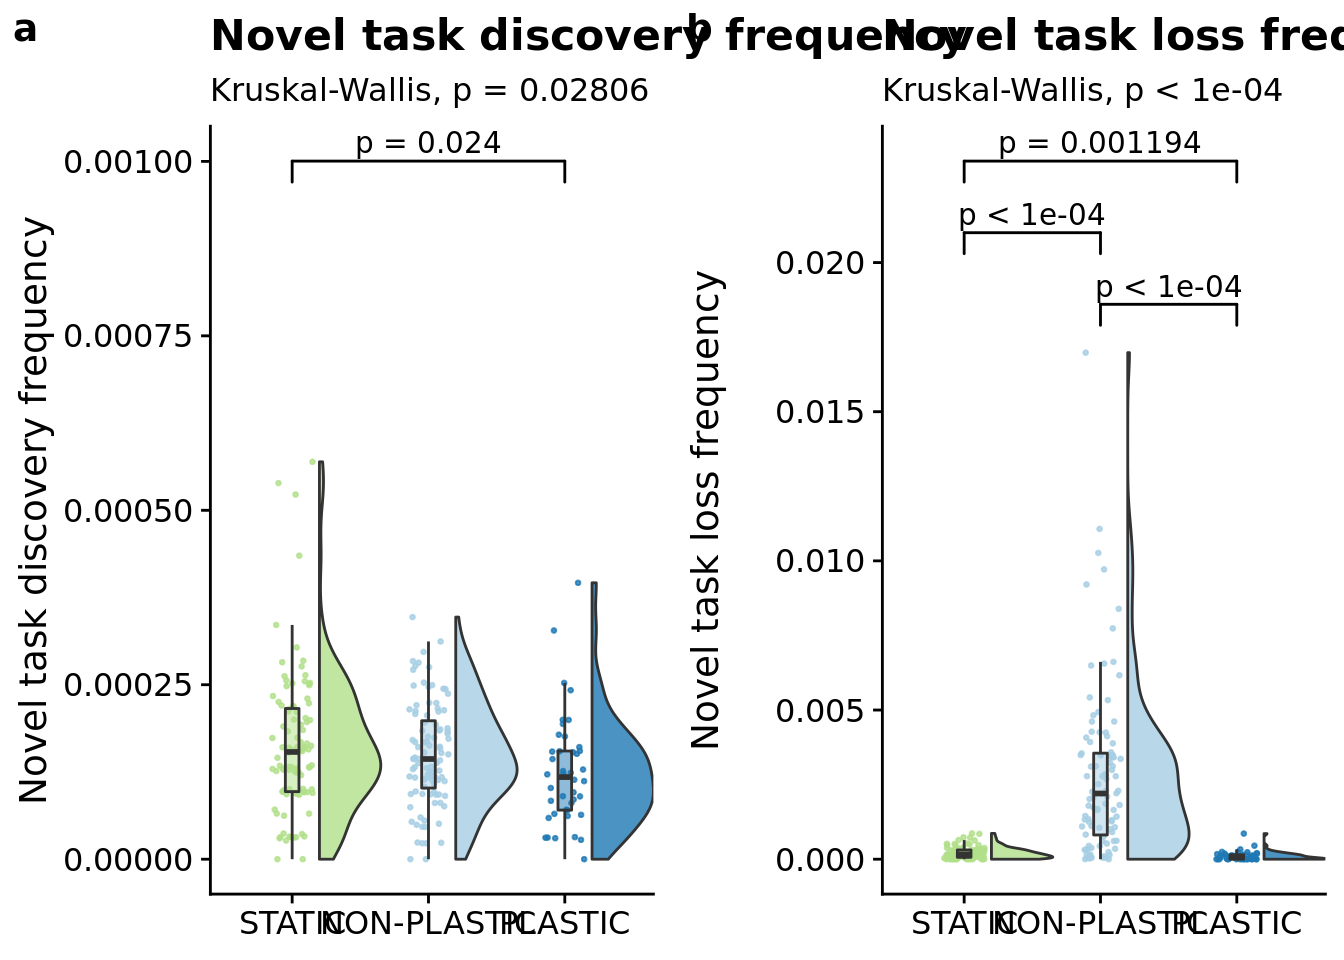
\includegraphics{supplemental-material_files/figure-latex/unnamed-chunk-69-2.pdf}

\begin{Shaded}
\begin{Highlighting}[]
\KeywordTok{save_plot}\NormalTok{(}
   \KeywordTok{paste0}\NormalTok{(working_directory, }\StringTok{"plots/"}\NormalTok{, }\StringTok{"complex-traits-magnitude-panel.pdf"}\NormalTok{),}
\NormalTok{   magnitude_grid,}
   \DataTypeTok{base_height=}\DecValTok{6}\NormalTok{,}
   \DataTypeTok{base_asp=}\DecValTok{3}\OperatorTok{/}\DecValTok{1}
\NormalTok{)}

\KeywordTok{save_plot}\NormalTok{(}
   \KeywordTok{paste0}\NormalTok{(working_directory, }\StringTok{"plots/"}\NormalTok{, }\StringTok{"complex-traits-pace-panel.pdf"}\NormalTok{),}
\NormalTok{   pace_grid,}
   \DataTypeTok{base_height=}\DecValTok{6}\NormalTok{,}
   \DataTypeTok{base_asp=}\DecValTok{2}\OperatorTok{/}\DecValTok{1}
\NormalTok{)}
\end{Highlighting}
\end{Shaded}

\hypertarget{accumulation-of-deleterious-instructions}{%
\chapter{Accumulation of deleterious instructions}\label{accumulation-of-deleterious-instructions}}

The effect of adaptive phenotypic plasticity on the accumulation of deleterious instructions.

\hypertarget{overview-3}{%
\section{Overview}\label{overview-3}}

\begin{Shaded}
\begin{Highlighting}[]
\NormalTok{total_updates <-}\StringTok{ }\DecValTok{200000}
\NormalTok{replicates <-}\StringTok{ }\DecValTok{100}
\NormalTok{alpha <-}\StringTok{ }\FloatTok{0.05}
\NormalTok{focal_poison_penalty <-}\StringTok{ }\FloatTok{0.1}

\NormalTok{focal_traits <-}\StringTok{ }\KeywordTok{c}\NormalTok{(}\StringTok{"not"}\NormalTok{,}\StringTok{"nand"}\NormalTok{,}\StringTok{"and"}\NormalTok{,}\StringTok{"ornot"}\NormalTok{,}\StringTok{"or"}\NormalTok{,}\StringTok{"andnot"}\NormalTok{)}
\NormalTok{traits_set_a <-}\StringTok{ }\KeywordTok{c}\NormalTok{(}\StringTok{"not"}\NormalTok{, }\StringTok{"and"}\NormalTok{, }\StringTok{"or"}\NormalTok{)}
\NormalTok{traits_set_b <-}\StringTok{ }\KeywordTok{c}\NormalTok{(}\StringTok{"nand"}\NormalTok{, }\StringTok{"ornot"}\NormalTok{, }\StringTok{"andnot"}\NormalTok{)}

\CommentTok{# Relative location of data.}
\NormalTok{working_directory <-}\StringTok{ "experiments/2021-02-05-hitchhiking/analysis/"} \CommentTok{# << For bookdown}
\CommentTok{# working_directory <- "./"}
\end{Highlighting}
\end{Shaded}

\hypertarget{analysis-dependencies-3}{%
\section{Analysis dependencies}\label{analysis-dependencies-3}}

Load all required R libraries.

\begin{Shaded}
\begin{Highlighting}[]
\KeywordTok{library}\NormalTok{(RColorBrewer)}
\KeywordTok{library}\NormalTok{(ggplot2)}
\KeywordTok{library}\NormalTok{(rstatix)}
\KeywordTok{library}\NormalTok{(ggsignif)}
\KeywordTok{library}\NormalTok{(scales)}
\KeywordTok{library}\NormalTok{(tidyverse)}
\KeywordTok{library}\NormalTok{(cowplot)}
\KeywordTok{library}\NormalTok{(Hmisc)}
\KeywordTok{library}\NormalTok{(boot)}
\KeywordTok{library}\NormalTok{(fmsb)}
\KeywordTok{library}\NormalTok{(knitr)}
\KeywordTok{source}\NormalTok{(}\StringTok{"https://gist.githubusercontent.com/benmarwick/2a1bb0133ff568cbe28d/raw/fb53bd97121f7f9ce947837ef1a4c65a73bffb3f/geom_flat_violin.R"}\NormalTok{)}
\end{Highlighting}
\end{Shaded}

These analyses were conducted/knitted with the following computing environment:

\begin{Shaded}
\begin{Highlighting}[]
\KeywordTok{print}\NormalTok{(version)}
\end{Highlighting}
\end{Shaded}

\begin{verbatim}
##                _                           
## platform       x86_64-pc-linux-gnu         
## arch           x86_64                      
## os             linux-gnu                   
## system         x86_64, linux-gnu           
## status                                     
## major          4                           
## minor          1.3                         
## year           2022                        
## month          03                          
## day            10                          
## svn rev        81868                       
## language       R                           
## version.string R version 4.1.3 (2022-03-10)
## nickname       One Push-Up
\end{verbatim}

\hypertarget{setup-3}{%
\section{Setup}\label{setup-3}}

\begin{Shaded}
\begin{Highlighting}[]
\CommentTok{####### summary data #######}
\NormalTok{summary_data_loc <-}\StringTok{ }\KeywordTok{paste0}\NormalTok{(working_directory, }\StringTok{"data/aggregate.csv"}\NormalTok{)}
\NormalTok{summary_data <-}\StringTok{ }\KeywordTok{read.csv}\NormalTok{(summary_data_loc, }\DataTypeTok{na.strings=}\StringTok{"NONE"}\NormalTok{)}

\NormalTok{summary_data}\OperatorTok{$}\NormalTok{DISABLE_REACTION_SENSORS <-}\StringTok{ }\KeywordTok{as.factor}\NormalTok{(summary_data}\OperatorTok{$}\NormalTok{DISABLE_REACTION_SENSORS)}
\NormalTok{summary_data}\OperatorTok{$}\NormalTok{chg_env <-}\StringTok{ }\NormalTok{summary_data}\OperatorTok{$}\NormalTok{chg_env }\OperatorTok{==}\StringTok{ "True"}
\NormalTok{summary_data}\OperatorTok{$}\NormalTok{dominant_plastic_odd_even <-}\StringTok{ }\KeywordTok{as.factor}\NormalTok{(summary_data}\OperatorTok{$}\NormalTok{dominant_plastic_odd_even)}
\NormalTok{summary_data}\OperatorTok{$}\NormalTok{sensors <-}\StringTok{ }\NormalTok{summary_data}\OperatorTok{$}\NormalTok{DISABLE_REACTION_SENSORS }\OperatorTok{==}\StringTok{ "0"}
\NormalTok{summary_data}\OperatorTok{$}\NormalTok{is_plastic <-}\StringTok{ }\NormalTok{summary_data}\OperatorTok{$}\NormalTok{dominant_plastic_odd_even }\OperatorTok{==}\StringTok{ "True"}
\NormalTok{summary_data}\OperatorTok{$}\NormalTok{POISON_PENALTY <-}\StringTok{ }\KeywordTok{as.factor}\NormalTok{(summary_data}\OperatorTok{$}\NormalTok{POISON_PENALTY)}

\NormalTok{summary_data}\OperatorTok{$}\NormalTok{dominant_lineage_num_times_hitchhike_inst_exec_increases_per_generation <-}\StringTok{ }\NormalTok{summary_data}\OperatorTok{$}\NormalTok{dominant_lineage_num_times_hitchhike_inst_exec_increases }\OperatorTok{/}\StringTok{ }\NormalTok{summary_data}\OperatorTok{$}\NormalTok{dominant_generation_born}
\NormalTok{summary_data}\OperatorTok{$}\NormalTok{frac_hitchhiking_linked_trait_change <-}\StringTok{ }\NormalTok{summary_data}\OperatorTok{$}\NormalTok{dominant_lineage_num_times_hitchhike_inst_exec_increases_with_primary_trait_change }\OperatorTok{/}\StringTok{ }\NormalTok{summary_data}\OperatorTok{$}\NormalTok{dominant_lineage_num_times_hitchhike_inst_exec_increases}
\NormalTok{summary_data}\OperatorTok{$}\NormalTok{frac_unexpressed_hitchhiker_inc <-}\StringTok{ }\NormalTok{summary_data}\OperatorTok{$}\NormalTok{dominant_lineage_num_times_hitchhike_inst_exec_increases_in_unexpressed_phenotype }\OperatorTok{/}\StringTok{ }\NormalTok{summary_data}\OperatorTok{$}\NormalTok{dominant_lineage_num_times_hitchhike_inst_exec_increases}
\NormalTok{summary_data}\OperatorTok{$}\NormalTok{frac_expressed_hitchiker_inc <-}\StringTok{ }\NormalTok{summary_data}\OperatorTok{$}\NormalTok{dominant_lineage_num_times_hitchhike_inst_exec_increases_in_expressed_phenotype }\OperatorTok{/}\StringTok{ }\NormalTok{summary_data}\OperatorTok{$}\NormalTok{dominant_lineage_num_times_hitchhike_inst_exec_increases}

\NormalTok{env_label_fun <-}\StringTok{ }\ControlFlowTok{function}\NormalTok{(chg_env) \{}
  \ControlFlowTok{if}\NormalTok{ (chg_env) \{}
    \KeywordTok{return}\NormalTok{(}\StringTok{"Fluctuating"}\NormalTok{)}
\NormalTok{  \} }\ControlFlowTok{else}\NormalTok{ \{}
    \KeywordTok{return}\NormalTok{(}\StringTok{"Constant"}\NormalTok{)}
\NormalTok{  \}}
\NormalTok{\}}

\NormalTok{sensors_label_fun <-}\StringTok{ }\ControlFlowTok{function}\NormalTok{(has_sensors) \{}
  \ControlFlowTok{if}\NormalTok{ (has_sensors) \{}
    \KeywordTok{return}\NormalTok{(}\StringTok{"Sensors"}\NormalTok{)}
\NormalTok{  \} }\ControlFlowTok{else}\NormalTok{ \{}
    \KeywordTok{return}\NormalTok{(}\StringTok{"No sensors"}\NormalTok{)}
\NormalTok{  \}}
\NormalTok{\}}

\NormalTok{condition_label_fun <-}\StringTok{ }\ControlFlowTok{function}\NormalTok{(has_sensors, env_chg) \{}
  \ControlFlowTok{if}\NormalTok{ (has_sensors }\OperatorTok{&&}\StringTok{ }\NormalTok{env_chg) \{}
    \KeywordTok{return}\NormalTok{(}\StringTok{"PLASTIC"}\NormalTok{)}
\NormalTok{  \} }\ControlFlowTok{else} \ControlFlowTok{if}\NormalTok{ (env_chg) \{}
    \KeywordTok{return}\NormalTok{(}\StringTok{"NON-PLASTIC"}\NormalTok{)}
\NormalTok{  \} }\ControlFlowTok{else}\NormalTok{ \{}
    \KeywordTok{return}\NormalTok{(}\StringTok{"STATIC"}\NormalTok{)}
\NormalTok{  \}}
\NormalTok{\}}

\NormalTok{summary_data}\OperatorTok{$}\NormalTok{env_label <-}\StringTok{ }\KeywordTok{mapply}\NormalTok{(}
\NormalTok{  env_label_fun,}
\NormalTok{  summary_data}\OperatorTok{$}\NormalTok{chg_env}
\NormalTok{)}
\NormalTok{summary_data}\OperatorTok{$}\NormalTok{sensors_label <-}\StringTok{ }\KeywordTok{mapply}\NormalTok{(}
\NormalTok{  sensors_label_fun,}
\NormalTok{  summary_data}\OperatorTok{$}\NormalTok{sensors}
\NormalTok{)}
\NormalTok{summary_data}\OperatorTok{$}\NormalTok{condition <-}\StringTok{ }\KeywordTok{mapply}\NormalTok{(}
\NormalTok{  condition_label_fun,}
\NormalTok{  summary_data}\OperatorTok{$}\NormalTok{sensors,}
\NormalTok{  summary_data}\OperatorTok{$}\NormalTok{chg_env}
\NormalTok{)}

\NormalTok{condition_order =}\StringTok{ }\KeywordTok{c}\NormalTok{(}
  \StringTok{"STATIC"}\NormalTok{,}
  \StringTok{"NON-PLASTIC"}\NormalTok{,}
  \StringTok{"PLASTIC"}
\NormalTok{)}

\NormalTok{pairwise_comparisons <-}\StringTok{ }\KeywordTok{list}\NormalTok{(}
  \KeywordTok{c}\NormalTok{(}\StringTok{"STATIC"}\NormalTok{, }\StringTok{"NON-PLASTIC"}\NormalTok{),}
  \KeywordTok{c}\NormalTok{(}\StringTok{"STATIC"}\NormalTok{, }\StringTok{"PLASTIC"}\NormalTok{),}
  \KeywordTok{c}\NormalTok{(}\StringTok{"PLASTIC"}\NormalTok{, }\StringTok{"NON-PLASTIC"}\NormalTok{)}
\NormalTok{)}

\NormalTok{p_label <-}\StringTok{ }\ControlFlowTok{function}\NormalTok{(p_value) \{}
\NormalTok{  threshold =}\StringTok{ }\FloatTok{0.0001}
  \ControlFlowTok{if}\NormalTok{ (p_value }\OperatorTok{<}\StringTok{ }\NormalTok{threshold) \{}
    \KeywordTok{return}\NormalTok{(}\KeywordTok{paste0}\NormalTok{(}\StringTok{"p < "}\NormalTok{, threshold))}
\NormalTok{  \} }\ControlFlowTok{else}\NormalTok{ \{}
    \KeywordTok{return}\NormalTok{(}\KeywordTok{paste0}\NormalTok{(}\StringTok{"p = "}\NormalTok{, p_value))}
\NormalTok{  \}}
\NormalTok{\}}

\NormalTok{poison_penalties <-}\StringTok{ }\KeywordTok{levels}\NormalTok{(summary_data}\OperatorTok{$}\NormalTok{POISON_PENALTY)}

\CommentTok{###### time series #####}
\NormalTok{lineage_time_series_data_loc <-}\StringTok{ }\KeywordTok{paste0}\NormalTok{(working_directory, }\StringTok{"data/lineage_series.csv"}\NormalTok{)}
\NormalTok{lineage_time_series_data <-}\StringTok{ }\KeywordTok{read.csv}\NormalTok{(lineage_time_series_data_loc)}

\NormalTok{lineage_time_series_data}\OperatorTok{$}\NormalTok{DISABLE_REACTION_SENSORS <-}\StringTok{ }\KeywordTok{as.factor}\NormalTok{(lineage_time_series_data}\OperatorTok{$}\NormalTok{DISABLE_REACTION_SENSORS)}
\NormalTok{lineage_time_series_data}\OperatorTok{$}\NormalTok{chg_env <-}\StringTok{ }\NormalTok{lineage_time_series_data}\OperatorTok{$}\NormalTok{chg_env }\OperatorTok{==}\StringTok{ "True"}
\NormalTok{lineage_time_series_data}\OperatorTok{$}\NormalTok{sensors <-}\StringTok{ }\NormalTok{lineage_time_series_data}\OperatorTok{$}\NormalTok{DISABLE_REACTION_SENSORS }\OperatorTok{==}\StringTok{ "0"}
\NormalTok{lineage_time_series_data}\OperatorTok{$}\NormalTok{POISON_PENALTY <-}\StringTok{ }\KeywordTok{as.factor}\NormalTok{(lineage_time_series_data}\OperatorTok{$}\NormalTok{POISON_VALUE)}

\NormalTok{lineage_time_series_data}\OperatorTok{$}\NormalTok{env_label <-}\StringTok{ }\KeywordTok{mapply}\NormalTok{(}
\NormalTok{  env_label_fun,}
\NormalTok{  lineage_time_series_data}\OperatorTok{$}\NormalTok{chg_env}
\NormalTok{)}
\NormalTok{lineage_time_series_data}\OperatorTok{$}\NormalTok{sensors_label <-}\StringTok{ }\KeywordTok{mapply}\NormalTok{(}
\NormalTok{  sensors_label_fun,}
\NormalTok{  lineage_time_series_data}\OperatorTok{$}\NormalTok{sensors}
\NormalTok{)}
\NormalTok{lineage_time_series_data}\OperatorTok{$}\NormalTok{condition <-}\StringTok{ }\KeywordTok{mapply}\NormalTok{(}
\NormalTok{  condition_label_fun,}
\NormalTok{  lineage_time_series_data}\OperatorTok{$}\NormalTok{sensors,}
\NormalTok{  lineage_time_series_data}\OperatorTok{$}\NormalTok{chg_env}
\NormalTok{)}

\CommentTok{####### misc #######}
\CommentTok{# Configure our default graphing theme}
\NormalTok{focal_summary_data <-}\StringTok{ }\KeywordTok{filter}\NormalTok{(summary_data, POISON_PENALTY}\OperatorTok{==}\NormalTok{focal_poison_penalty)}
\KeywordTok{theme_set}\NormalTok{(}\KeywordTok{theme_cowplot}\NormalTok{())}
\NormalTok{cb_palette <-}\StringTok{ "Paired"}
\KeywordTok{dir.create}\NormalTok{(}\KeywordTok{paste0}\NormalTok{(working_directory, }\StringTok{"plots"}\NormalTok{), }\DataTypeTok{showWarnings=}\OtherTok{FALSE}\NormalTok{)}
\NormalTok{samplemean <-}\StringTok{ }\ControlFlowTok{function}\NormalTok{(x, d) \{}
  \KeywordTok{return}\NormalTok{(}\KeywordTok{mean}\NormalTok{(x[d]))}
\NormalTok{\}}
\end{Highlighting}
\end{Shaded}

\hypertarget{evolution-of-phenotypic-plasticity-1}{%
\section{Evolution of phenotypic plasticity}\label{evolution-of-phenotypic-plasticity-1}}

For sensor-enabled populations in fluctuating environments, we only transfered populations containing an optimally plastic genotype to phase-two.

\begin{Shaded}
\begin{Highlighting}[]
\NormalTok{summary_data_grouped =}\StringTok{ }\NormalTok{dplyr}\OperatorTok{::}\KeywordTok{group_by}\NormalTok{(summary_data, sensors, env_label, condition, POISON_PENALTY)}
\NormalTok{summary_data_group_counts =}\StringTok{ }\NormalTok{dplyr}\OperatorTok{::}\KeywordTok{summarize}\NormalTok{(summary_data_grouped, }\DataTypeTok{n=}\NormalTok{dplyr}\OperatorTok{::}\KeywordTok{n}\NormalTok{())}

\KeywordTok{ggplot}\NormalTok{(summary_data_group_counts, }\KeywordTok{aes}\NormalTok{(}\DataTypeTok{x=}\NormalTok{condition, }\DataTypeTok{y=}\NormalTok{n, }\DataTypeTok{fill=}\NormalTok{condition)) }\OperatorTok{+}
\StringTok{  }\KeywordTok{geom_col}\NormalTok{(}\DataTypeTok{position=}\KeywordTok{position_dodge}\NormalTok{(}\FloatTok{0.9}\NormalTok{)) }\OperatorTok{+}
\StringTok{  }\KeywordTok{geom_text}\NormalTok{(}\KeywordTok{aes}\NormalTok{(}\DataTypeTok{label=}\NormalTok{n, }\DataTypeTok{y=}\NormalTok{n}\OperatorTok{+}\DecValTok{2}\NormalTok{)) }\OperatorTok{+}
\StringTok{  }\KeywordTok{scale_x_discrete}\NormalTok{(}
    \DataTypeTok{name=}\StringTok{"Condition"}\NormalTok{,}
    \DataTypeTok{limits=}\NormalTok{condition_order}
\NormalTok{  ) }\OperatorTok{+}
\StringTok{  }\KeywordTok{scale_fill_brewer}\NormalTok{(}
    \DataTypeTok{palette=}\NormalTok{cb_palette}
\NormalTok{  ) }\OperatorTok{+}
\StringTok{  }\KeywordTok{scale_color_brewer}\NormalTok{(}
    \DataTypeTok{palette=}\NormalTok{cb_palette}
\NormalTok{  ) }\OperatorTok{+}
\StringTok{  }\KeywordTok{ylab}\NormalTok{(}\StringTok{"Number of replicates in phase two"}\NormalTok{) }\OperatorTok{+}
\StringTok{  }\KeywordTok{facet_wrap}\NormalTok{(}\OperatorTok{~}\NormalTok{POISON_PENALTY, }\DataTypeTok{labeller=}\NormalTok{label_both) }\OperatorTok{+}
\StringTok{  }\KeywordTok{theme}\NormalTok{(}
    \DataTypeTok{legend.position=}\StringTok{"none"}
\NormalTok{  )}
\end{Highlighting}
\end{Shaded}

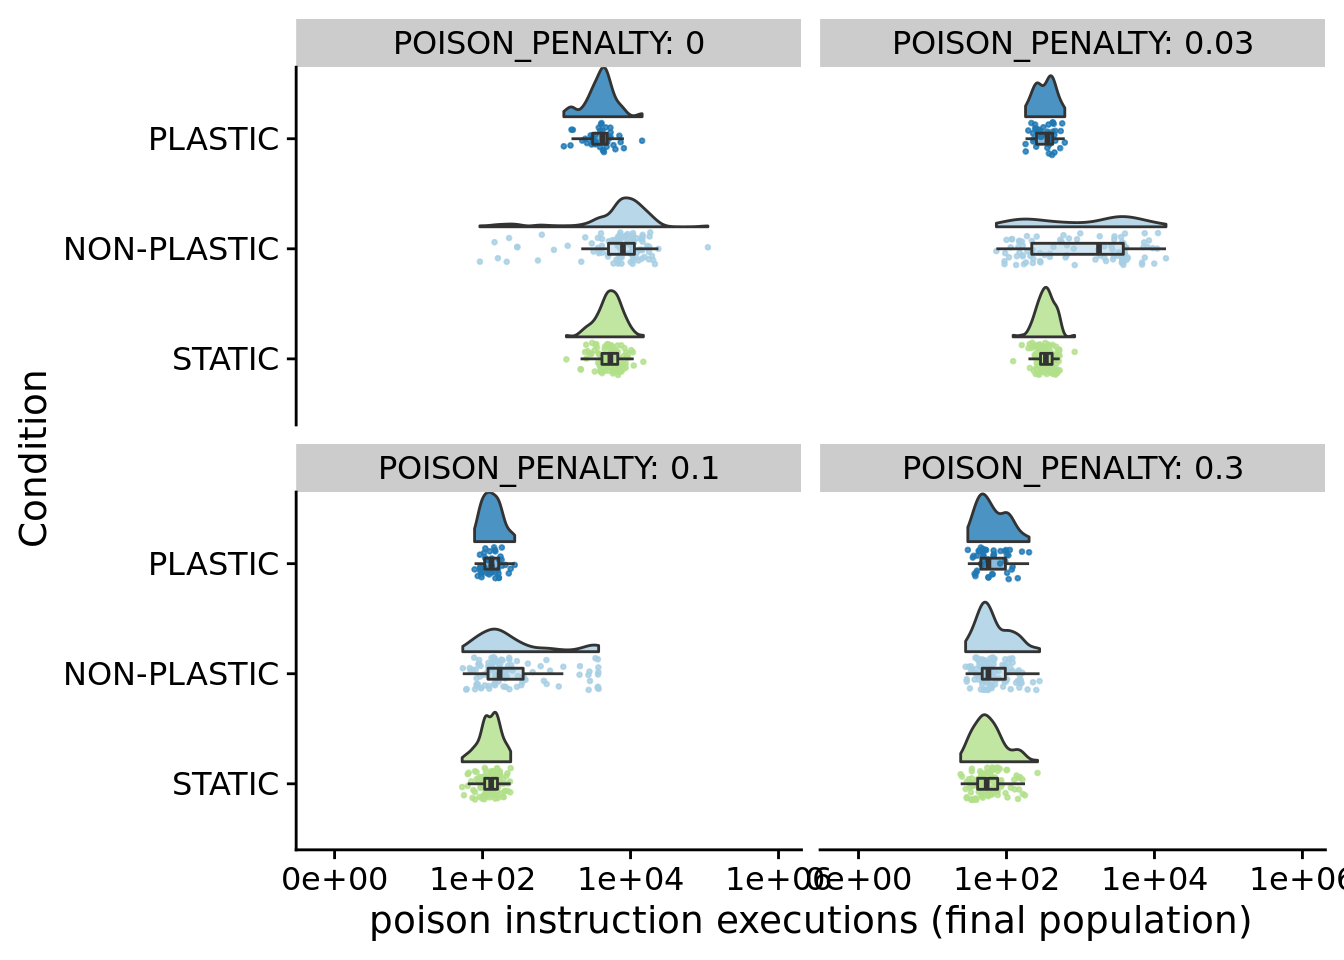
\includegraphics{supplemental-material_files/figure-latex/unnamed-chunk-74-1.pdf}

We can confirm our expectation that the dominant genotypes in non-plastic conditions are not phenotypically plastic.

\begin{Shaded}
\begin{Highlighting}[]
\NormalTok{summary_data_grouped =}\StringTok{ }\NormalTok{dplyr}\OperatorTok{::}\KeywordTok{group_by}\NormalTok{(summary_data, condition, is_plastic, POISON_PENALTY)}
\NormalTok{summary_data_group_counts =}\StringTok{ }\NormalTok{dplyr}\OperatorTok{::}\KeywordTok{summarize}\NormalTok{(summary_data_grouped, }\DataTypeTok{n=}\NormalTok{dplyr}\OperatorTok{::}\KeywordTok{n}\NormalTok{())}
\end{Highlighting}
\end{Shaded}

\begin{verbatim}
## `summarise()` has grouped output by 'condition', 'is_plastic'. You can override
## using the `.groups` argument.
\end{verbatim}

\begin{Shaded}
\begin{Highlighting}[]
\KeywordTok{ggplot}\NormalTok{(}\KeywordTok{filter}\NormalTok{(summary_data_group_counts, is_plastic), }\KeywordTok{aes}\NormalTok{(}\DataTypeTok{x=}\NormalTok{condition, }\DataTypeTok{y=}\NormalTok{n, }\DataTypeTok{fill=}\NormalTok{condition)) }\OperatorTok{+}
\StringTok{  }\KeywordTok{geom_col}\NormalTok{(}\DataTypeTok{position=}\KeywordTok{position_dodge}\NormalTok{(}\FloatTok{0.9}\NormalTok{)) }\OperatorTok{+}
\StringTok{  }\KeywordTok{scale_x_discrete}\NormalTok{(}
    \DataTypeTok{name=}\StringTok{"Condition"}\NormalTok{,}
    \DataTypeTok{limits=}\NormalTok{condition_order}
\NormalTok{  ) }\OperatorTok{+}
\StringTok{  }\KeywordTok{geom_text}\NormalTok{(}\KeywordTok{aes}\NormalTok{(}\DataTypeTok{label=}\NormalTok{n, }\DataTypeTok{y=}\NormalTok{n}\OperatorTok{+}\DecValTok{1}\NormalTok{)) }\OperatorTok{+}
\StringTok{  }\KeywordTok{scale_fill_brewer}\NormalTok{(}
    \DataTypeTok{palette=}\NormalTok{cb_palette}
\NormalTok{  ) }\OperatorTok{+}
\StringTok{  }\KeywordTok{scale_color_brewer}\NormalTok{(}
    \DataTypeTok{palette=}\NormalTok{cb_palette}
\NormalTok{  ) }\OperatorTok{+}
\StringTok{  }\KeywordTok{ylab}\NormalTok{(}\StringTok{"Number of replicates with a plastic dominant genotype"}\NormalTok{) }\OperatorTok{+}
\StringTok{  }\KeywordTok{ylim}\NormalTok{(}\DecValTok{0}\NormalTok{, }\DecValTok{100}\NormalTok{) }\OperatorTok{+}
\StringTok{  }\KeywordTok{facet_wrap}\NormalTok{(}\OperatorTok{~}\NormalTok{POISON_PENALTY, }\DataTypeTok{labeller=}\NormalTok{label_both) }\OperatorTok{+}
\StringTok{  }\KeywordTok{theme}\NormalTok{(}
    \DataTypeTok{legend.position=}\StringTok{"none"}
\NormalTok{  )}
\end{Highlighting}
\end{Shaded}

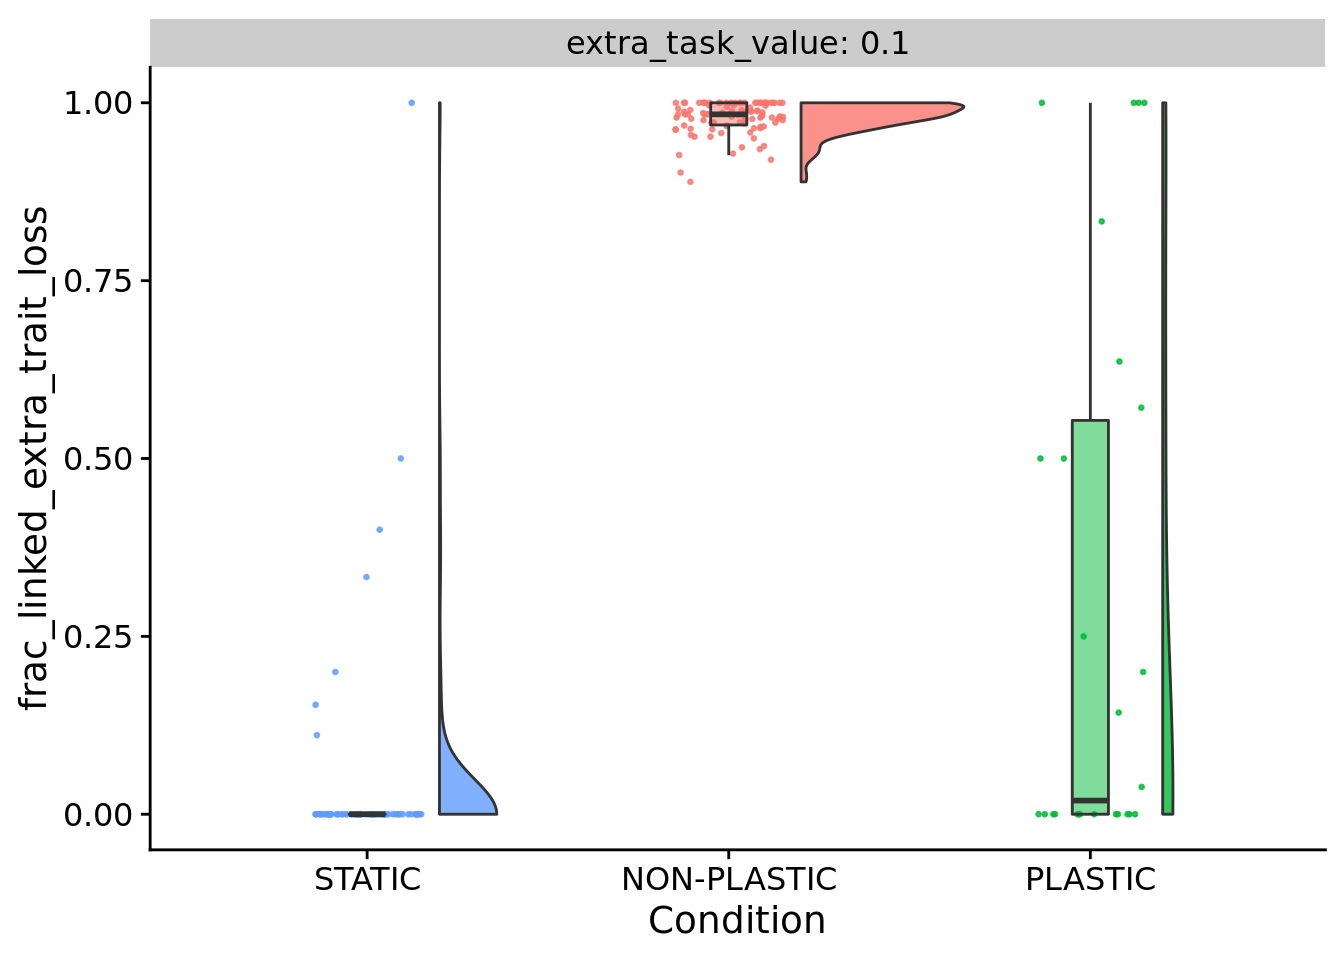
\includegraphics{supplemental-material_files/figure-latex/unnamed-chunk-75-1.pdf}

\hypertarget{deleterious-instruction-execution}{%
\section{Deleterious instruction execution}\label{deleterious-instruction-execution}}

Note that under the hood, the deleterious instruction is the \texttt{poison} instruction in Avida.

\hypertarget{number-of-replicates-where-final-dominant-genotype-executes-the-deleterious-instruction}{%
\subsection{Number of replicates where final dominant genotype executes the deleterious instruction}\label{number-of-replicates-where-final-dominant-genotype-executes-the-deleterious-instruction}}

\begin{Shaded}
\begin{Highlighting}[]
\ControlFlowTok{for}\NormalTok{ (penalty }\ControlFlowTok{in}\NormalTok{ poison_penalties) \{}
\NormalTok{  occurrences <-}\StringTok{ }\KeywordTok{c}\NormalTok{(}
    \KeywordTok{length}\NormalTok{(}\KeywordTok{filter}\NormalTok{(summary_data, POISON_PENALTY}\OperatorTok{==}\NormalTok{penalty }\OperatorTok{&}\StringTok{ }\NormalTok{condition}\OperatorTok{==}\StringTok{"NON-PLASTIC"} \OperatorTok{&}\StringTok{ }\NormalTok{dominant_times_poison_executed }\OperatorTok{>}\StringTok{ }\DecValTok{0}\NormalTok{)}\OperatorTok{$}\NormalTok{RANDOM_SEED),}
    \KeywordTok{length}\NormalTok{(}\KeywordTok{filter}\NormalTok{(summary_data, POISON_PENALTY}\OperatorTok{==}\NormalTok{penalty }\OperatorTok{&}\StringTok{ }\NormalTok{condition}\OperatorTok{==}\StringTok{"PLASTIC"} \OperatorTok{&}\StringTok{ }\NormalTok{dominant_times_poison_executed }\OperatorTok{>}\StringTok{ }\DecValTok{0}\NormalTok{)}\OperatorTok{$}\NormalTok{RANDOM_SEED),}
    \KeywordTok{length}\NormalTok{(}\KeywordTok{filter}\NormalTok{(summary_data, POISON_PENALTY}\OperatorTok{==}\NormalTok{penalty }\OperatorTok{&}\StringTok{ }\NormalTok{condition}\OperatorTok{==}\StringTok{"STATIC"} \OperatorTok{&}\StringTok{ }\NormalTok{dominant_times_poison_executed }\OperatorTok{>}\StringTok{ }\DecValTok{0}\NormalTok{)}\OperatorTok{$}\NormalTok{RANDOM_SEED)}
\NormalTok{  )}
\NormalTok{  trials <-}\StringTok{ }\KeywordTok{c}\NormalTok{(}
    \KeywordTok{length}\NormalTok{(}\KeywordTok{filter}\NormalTok{(summary_data, POISON_PENALTY}\OperatorTok{==}\NormalTok{penalty }\OperatorTok{&}\StringTok{ }\NormalTok{condition}\OperatorTok{==}\StringTok{"NON-PLASTIC"}\NormalTok{)}\OperatorTok{$}\NormalTok{RANDOM_SEED),}
    \KeywordTok{length}\NormalTok{(}\KeywordTok{filter}\NormalTok{(summary_data, POISON_PENALTY}\OperatorTok{==}\NormalTok{penalty }\OperatorTok{&}\StringTok{ }\NormalTok{condition}\OperatorTok{==}\StringTok{"PLASTIC"}\NormalTok{)}\OperatorTok{$}\NormalTok{RANDOM_SEED),}
    \KeywordTok{length}\NormalTok{(}\KeywordTok{filter}\NormalTok{(summary_data, POISON_PENALTY}\OperatorTok{==}\NormalTok{penalty }\OperatorTok{&}\StringTok{ }\NormalTok{condition}\OperatorTok{==}\StringTok{"STATIC"}\NormalTok{ )}\OperatorTok{$}\NormalTok{RANDOM_SEED)}
\NormalTok{  )}
  \KeywordTok{names}\NormalTok{(trials) <-}\StringTok{ }\KeywordTok{c}\NormalTok{(}
    \StringTok{"NON-PLASTIC"}\NormalTok{,}
    \StringTok{"PLASTIC"}\NormalTok{,}
    \StringTok{"STATIC"}
\NormalTok{  )}
  \KeywordTok{names}\NormalTok{(occurrences) <-}\StringTok{ }\KeywordTok{c}\NormalTok{(}
    \StringTok{"NON-PLASTIC"}\NormalTok{,}
    \StringTok{"PLASTIC"}\NormalTok{,}
    \StringTok{"STATIC"}
\NormalTok{  )}
\NormalTok{  poison_exec_table <-}\StringTok{ }\KeywordTok{data.frame}\NormalTok{(}
    \DataTypeTok{executes.poison=}\NormalTok{occurrences,}
    \DataTypeTok{replicates=}\NormalTok{trials}
\NormalTok{  )}
  \KeywordTok{cat}\NormalTok{(}\KeywordTok{paste0}\NormalTok{(}\StringTok{"#### Penalty: "}\NormalTok{, penalty, }\StringTok{"}\CharTok{\textbackslash{}n}\StringTok{"}\NormalTok{))}
  \KeywordTok{cat}\NormalTok{(}\KeywordTok{print}\NormalTok{(}\KeywordTok{kable}\NormalTok{(poison_exec_table)))}
  \KeywordTok{cat}\NormalTok{(}\StringTok{"}\CharTok{\textbackslash{}n}\StringTok{"}\NormalTok{)}
\NormalTok{  ft <-}\StringTok{ }\KeywordTok{pairwise.fisher.test}\NormalTok{(}\DataTypeTok{x=}\NormalTok{occurrences, }\DataTypeTok{n=}\NormalTok{trials, }\DataTypeTok{p.adjust.method=}\StringTok{"bonferroni"}\NormalTok{)}
  \KeywordTok{print}\NormalTok{(ft)}
  \KeywordTok{cat}\NormalTok{(}\StringTok{"}\CharTok{\textbackslash{}n\textbackslash{}n}\StringTok{"}\NormalTok{)}
\NormalTok{\}}
\end{Highlighting}
\end{Shaded}

\begin{verbatim}
## #### Penalty: 0
## 
## \begin{tabular}{l|r|r}
## \hline
##   & executes.poison & replicates\\
## \hline
## NON-PLASTIC & 86 & 100\\
## \hline
## PLASTIC & 27 & 41\\
## \hline
## STATIC & 85 & 100\\
## \hline
## \end{tabular}
## 
## 
##  Pairwise comparisons using Pairwise comparison of proportions (Fisher) 
## 
## data:  occurrences out of trials 
## 
##         NON-PLASTIC PLASTIC
## PLASTIC 0.03        -      
## STATIC  1.00        0.06   
## 
## P value adjustment method: bonferroni 
## 
## 
## #### Penalty: 0.03
## 
## \begin{tabular}{l|r|r}
## \hline
##   & executes.poison & replicates\\
## \hline
## NON-PLASTIC & 46 & 100\\
## \hline
## PLASTIC & 1 & 42\\
## \hline
## STATIC & 1 & 100\\
## \hline
## \end{tabular}
## 
## 
##  Pairwise comparisons using Pairwise comparison of proportions (Fisher) 
## 
## data:  occurrences out of trials 
## 
##         NON-PLASTIC PLASTIC
## PLASTIC 1.2e-07     -      
## STATIC  2.9e-15     1      
## 
## P value adjustment method: bonferroni 
## 
## 
## #### Penalty: 0.1
## 
## \begin{tabular}{l|r|r}
## \hline
##   & executes.poison & replicates\\
## \hline
## NON-PLASTIC & 14 & 100\\
## \hline
## PLASTIC & 0 & 43\\
## \hline
## STATIC & 0 & 100\\
## \hline
## \end{tabular}
## 
## 
##  Pairwise comparisons using Pairwise comparison of proportions (Fisher) 
## 
## data:  occurrences out of trials 
## 
##         NON-PLASTIC PLASTIC
## PLASTIC 0.03212     -      
## STATIC  0.00022     1.00000
## 
## P value adjustment method: bonferroni 
## 
## 
## #### Penalty: 0.3
## 
## \begin{tabular}{l|r|r}
## \hline
##   & executes.poison & replicates\\
## \hline
## NON-PLASTIC & 0 & 100\\
## \hline
## PLASTIC & 0 & 44\\
## \hline
## STATIC & 0 & 100\\
## \hline
## \end{tabular}
## 
## 
##  Pairwise comparisons using Pairwise comparison of proportions (Fisher) 
## 
## data:  occurrences out of trials 
## 
##         NON-PLASTIC PLASTIC
## PLASTIC 1           -      
## STATIC  1           1      
## 
## P value adjustment method: bonferroni
\end{verbatim}

\hypertarget{deleterious-instruction-execution-final-population}{%
\subsection{Deleterious instruction execution (final population)}\label{deleterious-instruction-execution-final-population}}

\begin{Shaded}
\begin{Highlighting}[]
\KeywordTok{ggplot}\NormalTok{(summary_data, }\KeywordTok{aes}\NormalTok{(}\DataTypeTok{x=}\NormalTok{condition, }\DataTypeTok{y=}\NormalTok{final_population_poison, }\DataTypeTok{fill=}\NormalTok{condition)) }\OperatorTok{+}
\StringTok{  }\KeywordTok{geom_flat_violin}\NormalTok{(}
    \DataTypeTok{position =} \KeywordTok{position_nudge}\NormalTok{(}\DataTypeTok{x =} \FloatTok{.2}\NormalTok{, }\DataTypeTok{y =} \DecValTok{0}\NormalTok{),}
    \DataTypeTok{alpha =} \FloatTok{.8}
\NormalTok{  ) }\OperatorTok{+}
\StringTok{  }\KeywordTok{geom_point}\NormalTok{(}
    \DataTypeTok{mapping=}\KeywordTok{aes}\NormalTok{(}\DataTypeTok{color=}\NormalTok{condition),}
    \DataTypeTok{position =} \KeywordTok{position_jitter}\NormalTok{(}\DataTypeTok{width =} \FloatTok{.15}\NormalTok{),}
    \DataTypeTok{size =} \FloatTok{.5}\NormalTok{,}
    \DataTypeTok{alpha =} \FloatTok{0.8}
\NormalTok{  ) }\OperatorTok{+}
\StringTok{  }\KeywordTok{geom_boxplot}\NormalTok{(}
    \DataTypeTok{width =} \FloatTok{.1}\NormalTok{,}
    \DataTypeTok{outlier.shape =} \OtherTok{NA}\NormalTok{,}
    \DataTypeTok{alpha =} \FloatTok{0.5}
\NormalTok{  ) }\OperatorTok{+}
\StringTok{  }\KeywordTok{scale_x_discrete}\NormalTok{(}
    \DataTypeTok{name=}\StringTok{"Condition"}\NormalTok{,}
    \DataTypeTok{limits=}\NormalTok{condition_order}
\NormalTok{  ) }\OperatorTok{+}
\StringTok{  }\KeywordTok{scale_y_continuous}\NormalTok{(}
    \DataTypeTok{name=}\StringTok{"deleterious instruction executions (final population)"}\NormalTok{,}
    \DataTypeTok{trans=}\KeywordTok{pseudo_log_trans}\NormalTok{(}\DataTypeTok{sigma=}\DecValTok{1}\NormalTok{,}\DataTypeTok{base=}\DecValTok{10}\NormalTok{),}
    \DataTypeTok{breaks=}\KeywordTok{c}\NormalTok{(}\DecValTok{0}\NormalTok{,}\DecValTok{100}\NormalTok{,}\DecValTok{10000}\NormalTok{,}\DecValTok{1000000}\NormalTok{),}
    \DataTypeTok{limits=}\KeywordTok{c}\NormalTok{(}\OperatorTok{-}\DecValTok{1}\NormalTok{,}\DecValTok{1000000}\NormalTok{)}
\NormalTok{  ) }\OperatorTok{+}
\StringTok{  }\KeywordTok{scale_fill_brewer}\NormalTok{(}
    \DataTypeTok{palette=}\NormalTok{cb_palette}
\NormalTok{  ) }\OperatorTok{+}
\StringTok{  }\KeywordTok{scale_color_brewer}\NormalTok{(}
    \DataTypeTok{palette=}\NormalTok{cb_palette}
\NormalTok{  ) }\OperatorTok{+}
\StringTok{  }\KeywordTok{facet_wrap}\NormalTok{(}
    \OperatorTok{~}\NormalTok{POISON_PENALTY,}
    \DataTypeTok{labeller=}\NormalTok{label_both}
\NormalTok{  ) }\OperatorTok{+}
\StringTok{  }\CommentTok{# coord_flip() +}
\StringTok{  }\KeywordTok{theme}\NormalTok{(}
    \DataTypeTok{legend.position=}\StringTok{"none"}
\NormalTok{  )}
\end{Highlighting}
\end{Shaded}

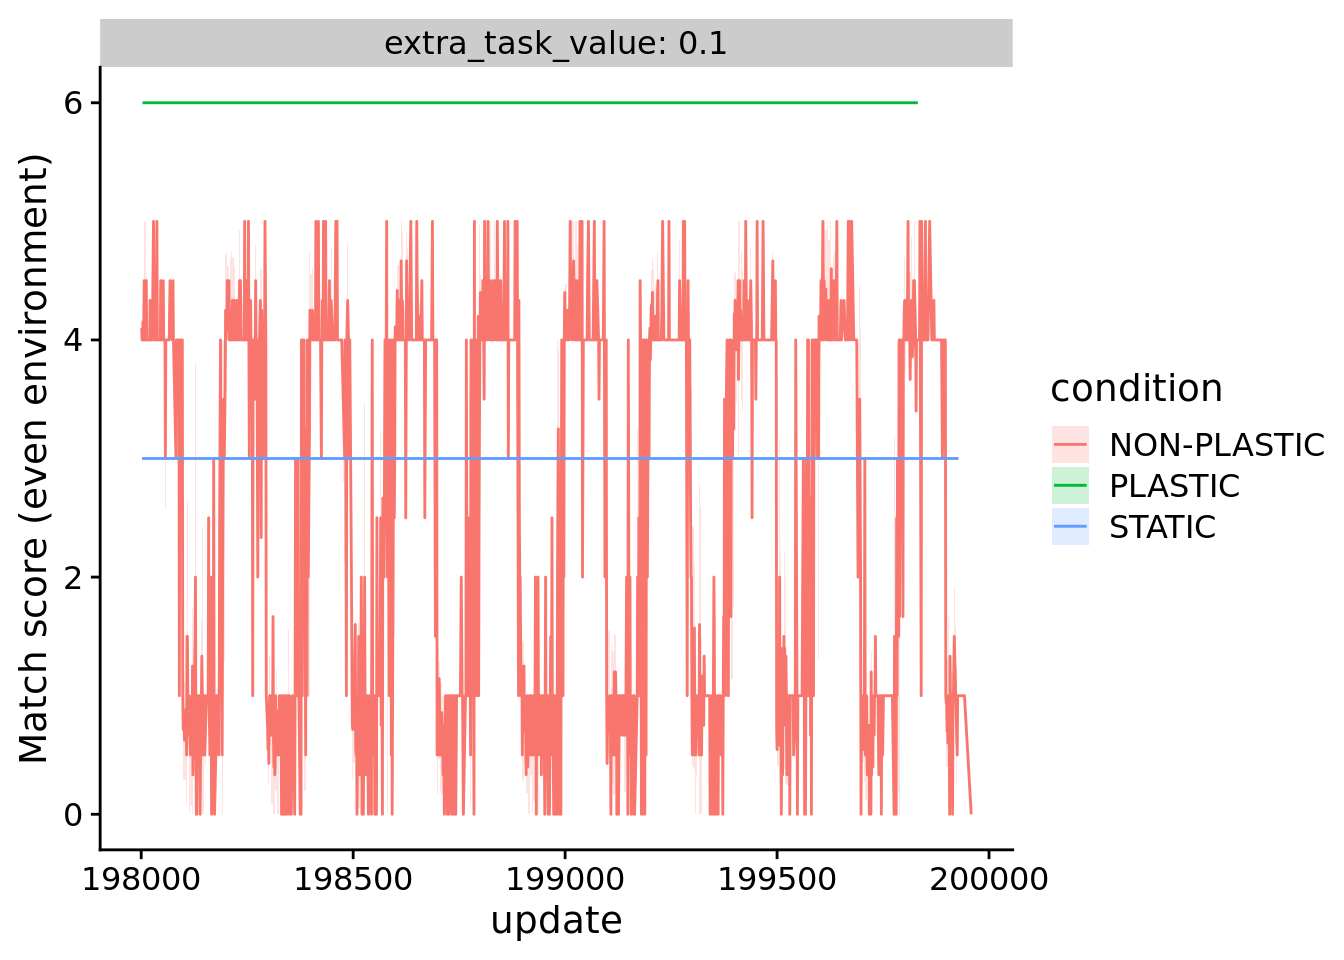
\includegraphics{supplemental-material_files/figure-latex/unnamed-chunk-77-1.pdf}

\begin{Shaded}
\begin{Highlighting}[]
\KeywordTok{ggsave}\NormalTok{(}
  \KeywordTok{paste0}\NormalTok{(working_directory, }\StringTok{"plots/final-population-poison-log.pdf"}\NormalTok{),}
  \DataTypeTok{width=}\DecValTok{15}\NormalTok{,}
  \DataTypeTok{height=}\DecValTok{10}
\NormalTok{)}
\end{Highlighting}
\end{Shaded}

\begin{Shaded}
\begin{Highlighting}[]
\ControlFlowTok{for}\NormalTok{ (penalty }\ControlFlowTok{in}\NormalTok{ poison_penalties) \{}
\NormalTok{  stat_data <-}\StringTok{ }\KeywordTok{filter}\NormalTok{(summary_data, POISON_PENALTY}\OperatorTok{==}\NormalTok{penalty)}
  \KeywordTok{print}\NormalTok{(}
    \KeywordTok{paste0}\NormalTok{(}
      \StringTok{"PENALTY: "}\NormalTok{, penalty}
\NormalTok{    )}
\NormalTok{  )}
\NormalTok{  kt <-}\StringTok{ }\KeywordTok{kruskal.test}\NormalTok{(}
      \DataTypeTok{formula=}\NormalTok{final_population_poison}\OperatorTok{~}\NormalTok{condition,}
      \DataTypeTok{data=}\NormalTok{stat_data}
\NormalTok{    )}
  \KeywordTok{print}\NormalTok{(}
\NormalTok{    kt}
\NormalTok{  )}
  \ControlFlowTok{if}\NormalTok{ (}\KeywordTok{is.na}\NormalTok{(kt}\OperatorTok{$}\NormalTok{p.value)) \{ }\ControlFlowTok{next}\NormalTok{ \}}
  \ControlFlowTok{if}\NormalTok{ (kt}\OperatorTok{$}\NormalTok{p.value }\OperatorTok{>}\StringTok{ }\FloatTok{0.05}\NormalTok{) \{ }\ControlFlowTok{next}\NormalTok{ \}}
  \KeywordTok{print}\NormalTok{(}
    \KeywordTok{pairwise.wilcox.test}\NormalTok{(}
      \DataTypeTok{x=}\NormalTok{stat_data}\OperatorTok{$}\NormalTok{final_population_poison,}
      \DataTypeTok{g=}\NormalTok{stat_data}\OperatorTok{$}\NormalTok{condition,}
      \DataTypeTok{p.adjust.method=}\StringTok{"bonferroni"}
\NormalTok{    )}
\NormalTok{  )}
\NormalTok{\}}
\end{Highlighting}
\end{Shaded}

\begin{verbatim}
## [1] "PENALTY: 0"
## 
##  Kruskal-Wallis rank sum test
## 
## data:  final_population_poison by condition
## Kruskal-Wallis chi-squared = 43.589, df = 2, p-value = 3.426e-10
## 
## 
##  Pairwise comparisons using Wilcoxon rank sum test with continuity correction 
## 
## data:  stat_data$final_population_poison and stat_data$condition 
## 
##         NON-PLASTIC PLASTIC
## PLASTIC 8.7e-07     -      
## STATIC  9.8e-07     0.00074
## 
## P value adjustment method: bonferroni 
## [1] "PENALTY: 0.03"
## 
##  Kruskal-Wallis rank sum test
## 
## data:  final_population_poison by condition
## Kruskal-Wallis chi-squared = 20.74, df = 2, p-value = 3.136e-05
## 
## 
##  Pairwise comparisons using Wilcoxon rank sum test with continuity correction 
## 
## data:  stat_data$final_population_poison and stat_data$condition 
## 
##         NON-PLASTIC PLASTIC
## PLASTIC 0.003       -      
## STATIC  1e-04       1.000  
## 
## P value adjustment method: bonferroni 
## [1] "PENALTY: 0.1"
## 
##  Kruskal-Wallis rank sum test
## 
## data:  final_population_poison by condition
## Kruskal-Wallis chi-squared = 20.608, df = 2, p-value = 3.35e-05
## 
## 
##  Pairwise comparisons using Wilcoxon rank sum test with continuity correction 
## 
## data:  stat_data$final_population_poison and stat_data$condition 
## 
##         NON-PLASTIC PLASTIC
## PLASTIC 0.0093      -      
## STATIC  4.9e-05     1.0000 
## 
## P value adjustment method: bonferroni 
## [1] "PENALTY: 0.3"
## 
##  Kruskal-Wallis rank sum test
## 
## data:  final_population_poison by condition
## Kruskal-Wallis chi-squared = 3.3994, df = 2, p-value = 0.1827
\end{verbatim}

\hypertarget{cummulative-deleterious-instruction-execution-along-final-dominant-lineages}{%
\subsection{Cummulative deleterious instruction execution along final dominant lineages}\label{cummulative-deleterious-instruction-execution-along-final-dominant-lineages}}

\begin{Shaded}
\begin{Highlighting}[]
\KeywordTok{ggplot}\NormalTok{(summary_data, }\KeywordTok{aes}\NormalTok{(}\DataTypeTok{x=}\NormalTok{condition, }\DataTypeTok{y=}\NormalTok{dominant_lineage_times_poison_executed, }\DataTypeTok{fill=}\NormalTok{condition)) }\OperatorTok{+}
\StringTok{  }\KeywordTok{geom_flat_violin}\NormalTok{(}
    \DataTypeTok{position =} \KeywordTok{position_nudge}\NormalTok{(}\DataTypeTok{x =} \FloatTok{.2}\NormalTok{, }\DataTypeTok{y =} \DecValTok{0}\NormalTok{),}
    \DataTypeTok{alpha =} \FloatTok{.8}
\NormalTok{  ) }\OperatorTok{+}
\StringTok{  }\KeywordTok{geom_point}\NormalTok{(}
    \DataTypeTok{mapping=}\KeywordTok{aes}\NormalTok{(}\DataTypeTok{color=}\NormalTok{condition),}
    \DataTypeTok{position =} \KeywordTok{position_jitter}\NormalTok{(}\DataTypeTok{width =} \FloatTok{.15}\NormalTok{),}
    \DataTypeTok{size =} \FloatTok{.5}\NormalTok{,}
    \DataTypeTok{alpha =} \FloatTok{0.8}
\NormalTok{  ) }\OperatorTok{+}
\StringTok{  }\KeywordTok{geom_boxplot}\NormalTok{(}
    \DataTypeTok{width =} \FloatTok{.1}\NormalTok{,}
    \DataTypeTok{outlier.shape =} \OtherTok{NA}\NormalTok{,}
    \DataTypeTok{alpha =} \FloatTok{0.5}
\NormalTok{  ) }\OperatorTok{+}
\StringTok{  }\KeywordTok{scale_x_discrete}\NormalTok{(}
    \DataTypeTok{name=}\StringTok{"Condition"}\NormalTok{,}
    \DataTypeTok{limits=}\NormalTok{condition_order}
\NormalTok{  ) }\OperatorTok{+}
\StringTok{  }\KeywordTok{scale_y_continuous}\NormalTok{(}
    \DataTypeTok{name=}\StringTok{"deleterious instruction executions (dominant lineage)"}\NormalTok{,}
    \DataTypeTok{trans=}\KeywordTok{pseudo_log_trans}\NormalTok{(}\DataTypeTok{sigma =} \DecValTok{1}\NormalTok{, }\DataTypeTok{base =} \DecValTok{10}\NormalTok{),}
    \DataTypeTok{breaks=}\KeywordTok{c}\NormalTok{(}\DecValTok{10}\NormalTok{,}\DecValTok{1000}\NormalTok{,}\DecValTok{100000}\NormalTok{),}
    \DataTypeTok{limits=}\KeywordTok{c}\NormalTok{(}\OperatorTok{-}\DecValTok{1}\NormalTok{,}\DecValTok{100000}\NormalTok{)}
\NormalTok{  ) }\OperatorTok{+}
\StringTok{  }\KeywordTok{facet_wrap}\NormalTok{(}
    \OperatorTok{~}\NormalTok{POISON_PENALTY,}
    \DataTypeTok{labeller=}\NormalTok{label_both}
\NormalTok{  ) }\OperatorTok{+}
\StringTok{  }\KeywordTok{scale_fill_brewer}\NormalTok{(}
    \DataTypeTok{palette=}\NormalTok{cb_palette}
\NormalTok{  ) }\OperatorTok{+}
\StringTok{  }\KeywordTok{scale_color_brewer}\NormalTok{(}
    \DataTypeTok{palette=}\NormalTok{cb_palette}
\NormalTok{  ) }\OperatorTok{+}
\StringTok{  }\KeywordTok{theme}\NormalTok{(}
    \DataTypeTok{legend.position=}\StringTok{"none"}
\NormalTok{  )}
\end{Highlighting}
\end{Shaded}

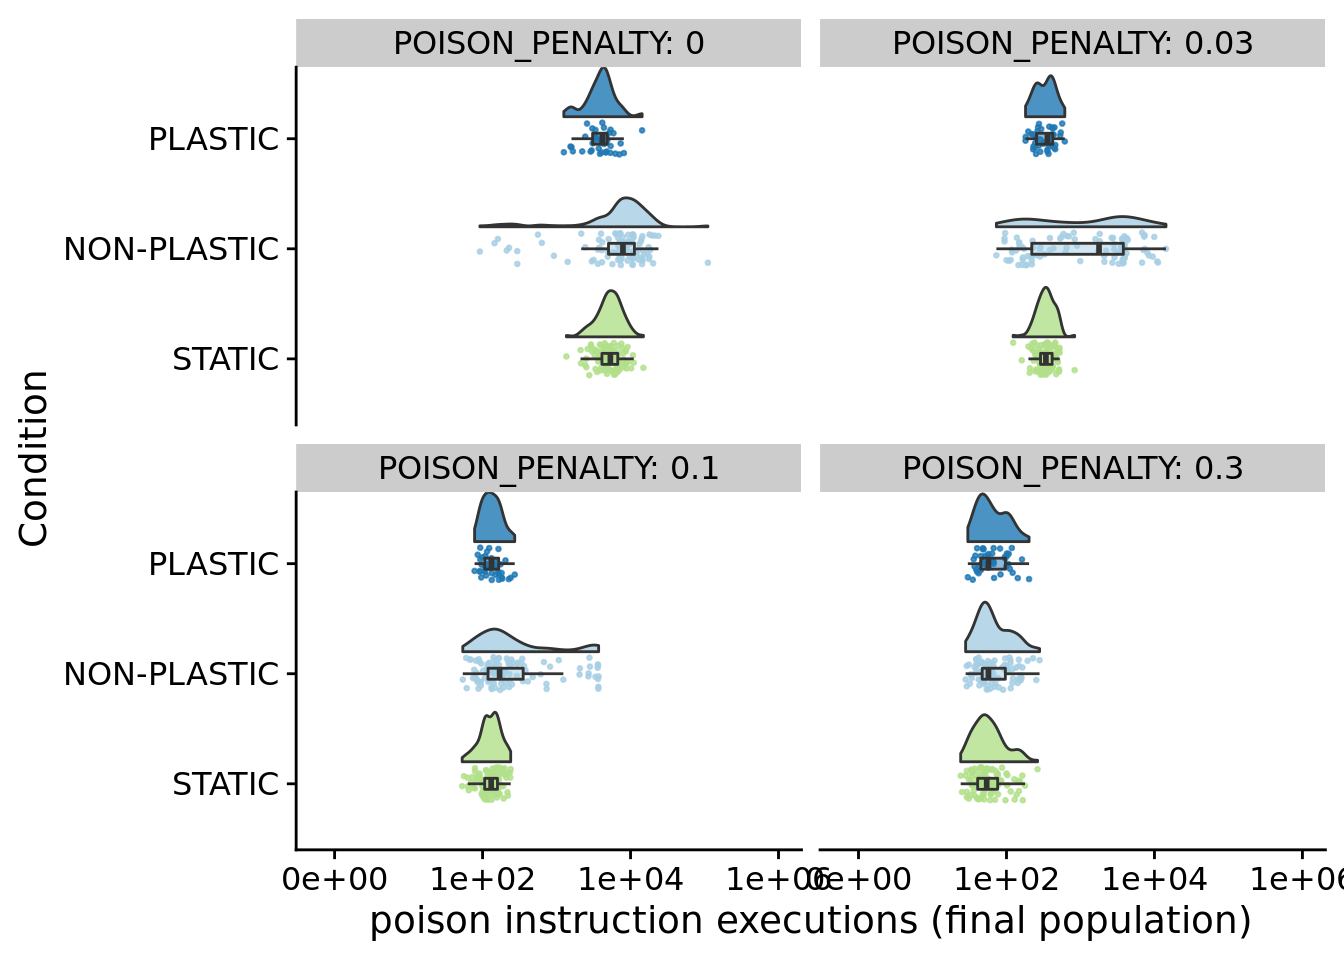
\includegraphics{supplemental-material_files/figure-latex/unnamed-chunk-79-1.pdf}

\begin{Shaded}
\begin{Highlighting}[]
\KeywordTok{ggsave}\NormalTok{(}
  \KeywordTok{paste0}\NormalTok{(working_directory, }\StringTok{"plots/final-dominant-lineage-poison-log.pdf"}\NormalTok{),}
  \DataTypeTok{width=}\DecValTok{15}\NormalTok{,}
  \DataTypeTok{height=}\DecValTok{10}
\NormalTok{)}
\end{Highlighting}
\end{Shaded}

\begin{Shaded}
\begin{Highlighting}[]
\ControlFlowTok{for}\NormalTok{ (penalty }\ControlFlowTok{in}\NormalTok{ poison_penalties) \{}
\NormalTok{  stat_data <-}\StringTok{ }\KeywordTok{filter}\NormalTok{(summary_data, POISON_PENALTY}\OperatorTok{==}\NormalTok{penalty)}
  \KeywordTok{print}\NormalTok{(}
    \KeywordTok{paste0}\NormalTok{(}
      \StringTok{"PENALTY: "}\NormalTok{, penalty}
\NormalTok{    )}
\NormalTok{  )}
\NormalTok{  kt <-}\StringTok{ }\KeywordTok{kruskal.test}\NormalTok{(}
      \DataTypeTok{formula=}\NormalTok{dominant_lineage_times_poison_executed}\OperatorTok{~}\NormalTok{condition,}
      \DataTypeTok{data=}\NormalTok{stat_data}
\NormalTok{    )}
  \KeywordTok{print}\NormalTok{(}
\NormalTok{    kt}
\NormalTok{  )}
  \ControlFlowTok{if}\NormalTok{ (}\KeywordTok{is.na}\NormalTok{(kt}\OperatorTok{$}\NormalTok{p.value)) \{ }\ControlFlowTok{next}\NormalTok{ \}}
  \ControlFlowTok{if}\NormalTok{ (kt}\OperatorTok{$}\NormalTok{p.value }\OperatorTok{>}\StringTok{ }\FloatTok{0.05}\NormalTok{) \{ }\ControlFlowTok{next}\NormalTok{ \}}
  \KeywordTok{print}\NormalTok{(}
    \KeywordTok{pairwise.wilcox.test}\NormalTok{(}
      \DataTypeTok{x=}\NormalTok{stat_data}\OperatorTok{$}\NormalTok{dominant_lineage_times_poison_executed,}
      \DataTypeTok{g=}\NormalTok{stat_data}\OperatorTok{$}\NormalTok{condition,}
      \DataTypeTok{p.adjust.method=}\StringTok{"bonferroni"}
\NormalTok{    )}
\NormalTok{  )}
\NormalTok{\}}
\end{Highlighting}
\end{Shaded}

\begin{verbatim}
## [1] "PENALTY: 0"
## 
##  Kruskal-Wallis rank sum test
## 
## data:  dominant_lineage_times_poison_executed by condition
## Kruskal-Wallis chi-squared = 178.84, df = 2, p-value < 2.2e-16
## 
## 
##  Pairwise comparisons using Wilcoxon rank sum test with continuity correction 
## 
## data:  stat_data$dominant_lineage_times_poison_executed and stat_data$condition 
## 
##         NON-PLASTIC PLASTIC
## PLASTIC <2e-16      -      
## STATIC  <2e-16      0.0018 
## 
## P value adjustment method: bonferroni 
## [1] "PENALTY: 0.03"
## 
##  Kruskal-Wallis rank sum test
## 
## data:  dominant_lineage_times_poison_executed by condition
## Kruskal-Wallis chi-squared = 178.62, df = 2, p-value < 2.2e-16
## 
## 
##  Pairwise comparisons using Wilcoxon rank sum test with continuity correction 
## 
## data:  stat_data$dominant_lineage_times_poison_executed and stat_data$condition 
## 
##         NON-PLASTIC PLASTIC
## PLASTIC <2e-16      -      
## STATIC  <2e-16      0.011  
## 
## P value adjustment method: bonferroni 
## [1] "PENALTY: 0.1"
## 
##  Kruskal-Wallis rank sum test
## 
## data:  dominant_lineage_times_poison_executed by condition
## Kruskal-Wallis chi-squared = 184.83, df = 2, p-value < 2.2e-16
## 
## 
##  Pairwise comparisons using Wilcoxon rank sum test with continuity correction 
## 
## data:  stat_data$dominant_lineage_times_poison_executed and stat_data$condition 
## 
##         NON-PLASTIC PLASTIC
## PLASTIC <2e-16      -      
## STATIC  <2e-16      0.21   
## 
## P value adjustment method: bonferroni 
## [1] "PENALTY: 0.3"
## 
##  Kruskal-Wallis rank sum test
## 
## data:  dominant_lineage_times_poison_executed by condition
## Kruskal-Wallis chi-squared = 149.48, df = 2, p-value < 2.2e-16
## 
## 
##  Pairwise comparisons using Wilcoxon rank sum test with continuity correction 
## 
## data:  stat_data$dominant_lineage_times_poison_executed and stat_data$condition 
## 
##         NON-PLASTIC PLASTIC
## PLASTIC 4.4e-16     -      
## STATIC  < 2e-16     0.84   
## 
## P value adjustment method: bonferroni
\end{verbatim}

\hypertarget{characterizing-mutations-that-increase-deleterious-instruction-execution}{%
\section{Characterizing mutations that increase deleterious instruction execution}\label{characterizing-mutations-that-increase-deleterious-instruction-execution}}

\hypertarget{number-of-offspring-along-dominant-lineage-with-increase-in-deleterious-instruction-execution}{%
\subsection{Number of offspring along dominant lineage with increase in deleterious instruction execution}\label{number-of-offspring-along-dominant-lineage-with-increase-in-deleterious-instruction-execution}}

\begin{Shaded}
\begin{Highlighting}[]
\KeywordTok{ggplot}\NormalTok{(summary_data, }\KeywordTok{aes}\NormalTok{(}\DataTypeTok{x=}\NormalTok{condition, }\DataTypeTok{y=}\NormalTok{dominant_lineage_num_times_hitchhike_inst_exec_increases, }\DataTypeTok{fill=}\NormalTok{condition)) }\OperatorTok{+}
\StringTok{  }\KeywordTok{geom_flat_violin}\NormalTok{(}
    \DataTypeTok{position =} \KeywordTok{position_nudge}\NormalTok{(}\DataTypeTok{x =} \FloatTok{.2}\NormalTok{, }\DataTypeTok{y =} \DecValTok{0}\NormalTok{),}
    \DataTypeTok{alpha =} \FloatTok{.8}
\NormalTok{  ) }\OperatorTok{+}
\StringTok{  }\KeywordTok{geom_point}\NormalTok{(}
    \DataTypeTok{mapping=}\KeywordTok{aes}\NormalTok{(}\DataTypeTok{color=}\NormalTok{condition),}
    \DataTypeTok{position =} \KeywordTok{position_jitter}\NormalTok{(}\DataTypeTok{width =} \FloatTok{.15}\NormalTok{),}
    \DataTypeTok{size =} \FloatTok{.5}\NormalTok{,}
    \DataTypeTok{alpha =} \FloatTok{0.8}
\NormalTok{  ) }\OperatorTok{+}
\StringTok{  }\KeywordTok{geom_boxplot}\NormalTok{(}
    \DataTypeTok{width =} \FloatTok{.1}\NormalTok{,}
    \DataTypeTok{outlier.shape =} \OtherTok{NA}\NormalTok{,}
    \DataTypeTok{alpha =} \FloatTok{0.5}
\NormalTok{  ) }\OperatorTok{+}
\StringTok{  }\KeywordTok{scale_x_discrete}\NormalTok{(}
    \DataTypeTok{name=}\StringTok{"Condition"}\NormalTok{,}
    \DataTypeTok{limits=}\NormalTok{condition_order}
\NormalTok{  ) }\OperatorTok{+}
\StringTok{  }\KeywordTok{facet_wrap}\NormalTok{(}
    \OperatorTok{~}\NormalTok{POISON_PENALTY,}
    \DataTypeTok{labeller=}\NormalTok{label_both}
\NormalTok{  ) }\OperatorTok{+}
\StringTok{  }\KeywordTok{scale_fill_brewer}\NormalTok{(}
    \DataTypeTok{palette=}\NormalTok{cb_palette}
\NormalTok{  ) }\OperatorTok{+}
\StringTok{  }\KeywordTok{scale_color_brewer}\NormalTok{(}
    \DataTypeTok{palette=}\NormalTok{cb_palette}
\NormalTok{  ) }\OperatorTok{+}
\StringTok{  }\KeywordTok{theme}\NormalTok{(}
    \DataTypeTok{legend.position=}\StringTok{"none"}
\NormalTok{  )}
\end{Highlighting}
\end{Shaded}

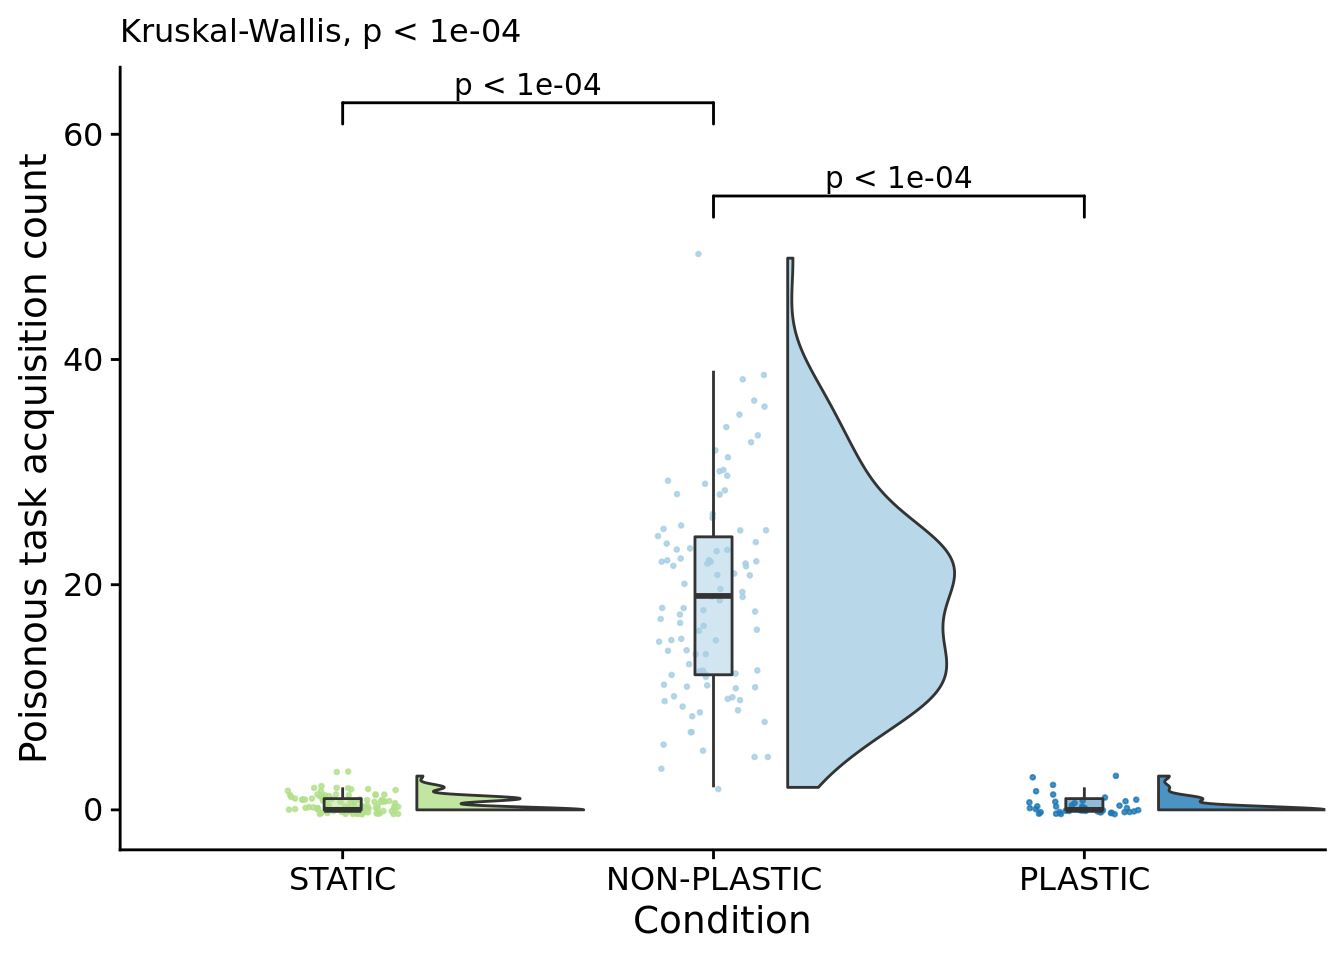
\includegraphics{supplemental-material_files/figure-latex/unnamed-chunk-81-1.pdf}

\begin{Shaded}
\begin{Highlighting}[]
\ControlFlowTok{for}\NormalTok{ (penalty }\ControlFlowTok{in}\NormalTok{ poison_penalties) \{}
\NormalTok{  stat_data <-}\StringTok{ }\KeywordTok{filter}\NormalTok{(summary_data, POISON_PENALTY}\OperatorTok{==}\NormalTok{penalty)}
  \KeywordTok{print}\NormalTok{(}
    \KeywordTok{paste0}\NormalTok{(}
      \StringTok{"PENALTY: "}\NormalTok{, penalty}
\NormalTok{    )}
\NormalTok{  )}
\NormalTok{  kt <-}\StringTok{ }\KeywordTok{kruskal.test}\NormalTok{(}
      \DataTypeTok{formula=}\NormalTok{dominant_lineage_num_times_hitchhike_inst_exec_increases}\OperatorTok{~}\NormalTok{condition,}
      \DataTypeTok{data=}\NormalTok{stat_data}
\NormalTok{    )}
  \KeywordTok{print}\NormalTok{(}
\NormalTok{    kt}
\NormalTok{  )}
  \ControlFlowTok{if}\NormalTok{ (}\KeywordTok{is.na}\NormalTok{(kt}\OperatorTok{$}\NormalTok{p.value)) \{ }\ControlFlowTok{next}\NormalTok{ \}}
  \ControlFlowTok{if}\NormalTok{ (kt}\OperatorTok{$}\NormalTok{p.value }\OperatorTok{>}\StringTok{ }\FloatTok{0.05}\NormalTok{) \{ }\ControlFlowTok{next}\NormalTok{ \}}
  \KeywordTok{print}\NormalTok{(}
    \KeywordTok{pairwise.wilcox.test}\NormalTok{(}
      \DataTypeTok{x=}\NormalTok{stat_data}\OperatorTok{$}\NormalTok{dominant_lineage_num_times_hitchhike_inst_exec_increases,}
      \DataTypeTok{g=}\NormalTok{stat_data}\OperatorTok{$}\NormalTok{condition,}
      \DataTypeTok{p.adjust.method=}\StringTok{"bonferroni"}
\NormalTok{    )}
\NormalTok{  )}
\NormalTok{\}}
\end{Highlighting}
\end{Shaded}

\begin{verbatim}
## [1] "PENALTY: 0"
## 
##  Kruskal-Wallis rank sum test
## 
## data:  dominant_lineage_num_times_hitchhike_inst_exec_increases by condition
## Kruskal-Wallis chi-squared = 179.79, df = 2, p-value < 2.2e-16
## 
## 
##  Pairwise comparisons using Wilcoxon rank sum test with continuity correction 
## 
## data:  stat_data$dominant_lineage_num_times_hitchhike_inst_exec_increases and stat_data$condition 
## 
##         NON-PLASTIC PLASTIC
## PLASTIC < 2e-16     -      
## STATIC  < 2e-16     0.00046
## 
## P value adjustment method: bonferroni 
## [1] "PENALTY: 0.03"
## 
##  Kruskal-Wallis rank sum test
## 
## data:  dominant_lineage_num_times_hitchhike_inst_exec_increases by condition
## Kruskal-Wallis chi-squared = 179.35, df = 2, p-value < 2.2e-16
## 
## 
##  Pairwise comparisons using Wilcoxon rank sum test with continuity correction 
## 
## data:  stat_data$dominant_lineage_num_times_hitchhike_inst_exec_increases and stat_data$condition 
## 
##         NON-PLASTIC PLASTIC
## PLASTIC <2e-16      -      
## STATIC  <2e-16      0.03   
## 
## P value adjustment method: bonferroni 
## [1] "PENALTY: 0.1"
## 
##  Kruskal-Wallis rank sum test
## 
## data:  dominant_lineage_num_times_hitchhike_inst_exec_increases by condition
## Kruskal-Wallis chi-squared = 185.34, df = 2, p-value < 2.2e-16
## 
## 
##  Pairwise comparisons using Wilcoxon rank sum test with continuity correction 
## 
## data:  stat_data$dominant_lineage_num_times_hitchhike_inst_exec_increases and stat_data$condition 
## 
##         NON-PLASTIC PLASTIC
## PLASTIC <2e-16      -      
## STATIC  <2e-16      0.27   
## 
## P value adjustment method: bonferroni 
## [1] "PENALTY: 0.3"
## 
##  Kruskal-Wallis rank sum test
## 
## data:  dominant_lineage_num_times_hitchhike_inst_exec_increases by condition
## Kruskal-Wallis chi-squared = 146.35, df = 2, p-value < 2.2e-16
## 
## 
##  Pairwise comparisons using Wilcoxon rank sum test with continuity correction 
## 
## data:  stat_data$dominant_lineage_num_times_hitchhike_inst_exec_increases and stat_data$condition 
## 
##         NON-PLASTIC PLASTIC
## PLASTIC 7.8e-16     -      
## STATIC  < 2e-16     0.86   
## 
## P value adjustment method: bonferroni
\end{verbatim}

Focal figure for the manuscript:

\begin{Shaded}
\begin{Highlighting}[]
\CommentTok{# Compute manual labels for geom_signif}
\NormalTok{stat.test <-}\StringTok{ }\NormalTok{focal_summary_data }\OperatorTok
\StringTok{  }\KeywordTok{wilcox_test}\NormalTok{(dominant_lineage_num_times_hitchhike_inst_exec_increases }\OperatorTok{~}\StringTok{ }\NormalTok{condition) }\OperatorTok
\StringTok{  }\KeywordTok{adjust_pvalue}\NormalTok{(}\DataTypeTok{method =} \StringTok{"bonferroni"}\NormalTok{) }\OperatorTok
\StringTok{  }\KeywordTok{add_significance}\NormalTok{() }\OperatorTok
\StringTok{  }\KeywordTok{add_xy_position}\NormalTok{(}\DataTypeTok{x=}\StringTok{"condition"}\NormalTok{)}
\CommentTok{# Tweak y.position manually to account for scaled axis (edge case that triggers bad behavior in geom_signif)}
\NormalTok{stat.test}\OperatorTok{$}\NormalTok{manual_position <-}\StringTok{  }\NormalTok{stat.test}\OperatorTok{$}\NormalTok{y.position}
\NormalTok{stat.test}\OperatorTok{$}\NormalTok{label <-}\StringTok{ }\KeywordTok{mapply}\NormalTok{(p_label,stat.test}\OperatorTok{$}\NormalTok{p.adj)}

\NormalTok{poison_increases_fig <-}\StringTok{ }\KeywordTok{ggplot}\NormalTok{(}
\NormalTok{    focal_summary_data,}
    \KeywordTok{aes}\NormalTok{(}\DataTypeTok{x=}\NormalTok{condition, }\DataTypeTok{y=}\NormalTok{dominant_lineage_num_times_hitchhike_inst_exec_increases, }\DataTypeTok{fill=}\NormalTok{condition)}
\NormalTok{  ) }\OperatorTok{+}
\StringTok{  }\KeywordTok{geom_flat_violin}\NormalTok{(}
    \DataTypeTok{scale=}\StringTok{"width"}\NormalTok{,}
    \DataTypeTok{position =} \KeywordTok{position_nudge}\NormalTok{(}\DataTypeTok{x =} \FloatTok{.2}\NormalTok{, }\DataTypeTok{y =} \DecValTok{0}\NormalTok{),}
    \DataTypeTok{alpha =} \FloatTok{.8}
\NormalTok{  ) }\OperatorTok{+}
\StringTok{  }\KeywordTok{geom_point}\NormalTok{(}
    \DataTypeTok{mapping=}\KeywordTok{aes}\NormalTok{(}\DataTypeTok{color=}\NormalTok{condition),}
    \DataTypeTok{position =} \KeywordTok{position_jitter}\NormalTok{(}\DataTypeTok{width =} \FloatTok{.15}\NormalTok{),}
    \DataTypeTok{size =} \FloatTok{.5}\NormalTok{,}
    \DataTypeTok{alpha =} \FloatTok{0.8}
\NormalTok{  ) }\OperatorTok{+}
\StringTok{  }\KeywordTok{geom_boxplot}\NormalTok{(}
    \DataTypeTok{width =} \FloatTok{.1}\NormalTok{,}
    \DataTypeTok{outlier.shape =} \OtherTok{NA}\NormalTok{,}
    \DataTypeTok{alpha =} \FloatTok{0.5}
\NormalTok{  ) }\OperatorTok{+}
\StringTok{  }\KeywordTok{scale_x_discrete}\NormalTok{(}
    \DataTypeTok{name=}\StringTok{"Condition"}\NormalTok{,}
    \DataTypeTok{limits=}\NormalTok{condition_order,}
    \DataTypeTok{labels=}\NormalTok{condition_order}
\NormalTok{  ) }\OperatorTok{+}
\StringTok{  }\KeywordTok{scale_y_continuous}\NormalTok{(}
    \DataTypeTok{name=}\StringTok{"Deleterious function acquisition count"}\NormalTok{,}
\NormalTok{  ) }\OperatorTok{+}
\StringTok{  }\KeywordTok{scale_fill_brewer}\NormalTok{(}
    \DataTypeTok{palette=}\NormalTok{cb_palette}
\NormalTok{  ) }\OperatorTok{+}
\StringTok{  }\KeywordTok{scale_color_brewer}\NormalTok{(}
    \DataTypeTok{palette=}\NormalTok{cb_palette}
\NormalTok{  ) }\OperatorTok{+}
\StringTok{  }\CommentTok{# coord_flip()}
\StringTok{  }\KeywordTok{labs}\NormalTok{(}
    \DataTypeTok{subtitle=}\KeywordTok{paste0}\NormalTok{(}
      \StringTok{"Kruskal-Wallis, "}\NormalTok{,}
      \KeywordTok{p_label}\NormalTok{(}\KeywordTok{signif}\NormalTok{(}\KeywordTok{kruskal.test}\NormalTok{(}\DataTypeTok{formula=}\NormalTok{dominant_lineage_num_times_hitchhike_inst_exec_increases}\OperatorTok{~}\NormalTok{condition, }\DataTypeTok{data=}\NormalTok{focal_summary_data)}\OperatorTok{$}\NormalTok{p.value,}\DataTypeTok{digits=}\DecValTok{4}\NormalTok{))}
\NormalTok{    )}
\NormalTok{  ) }\OperatorTok{+}
\StringTok{  }\NormalTok{ggsignif}\OperatorTok{::}\KeywordTok{geom_signif}\NormalTok{(}
    \DataTypeTok{data=}\KeywordTok{filter}\NormalTok{(stat.test, p.adj }\OperatorTok{<=}\StringTok{ }\NormalTok{alpha),}
    \KeywordTok{aes}\NormalTok{(}\DataTypeTok{xmin=}\NormalTok{group1,}\DataTypeTok{xmax=}\NormalTok{group2,}\DataTypeTok{annotations=}\NormalTok{label,}\DataTypeTok{y_position=}\NormalTok{manual_position),}
    \DataTypeTok{manual=}\OtherTok{TRUE}\NormalTok{,}
    \DataTypeTok{inherit.aes=}\OtherTok{FALSE}
\NormalTok{  ) }\OperatorTok{+}
\StringTok{  }\KeywordTok{theme}\NormalTok{(}
    \DataTypeTok{legend.position=}\StringTok{"none"}
\NormalTok{  )}
\end{Highlighting}
\end{Shaded}

\begin{verbatim}
## Warning: Ignoring unknown aesthetics: xmin, xmax, annotations, y_position
\end{verbatim}

\begin{Shaded}
\begin{Highlighting}[]
\NormalTok{poison_increases_fig}
\end{Highlighting}
\end{Shaded}

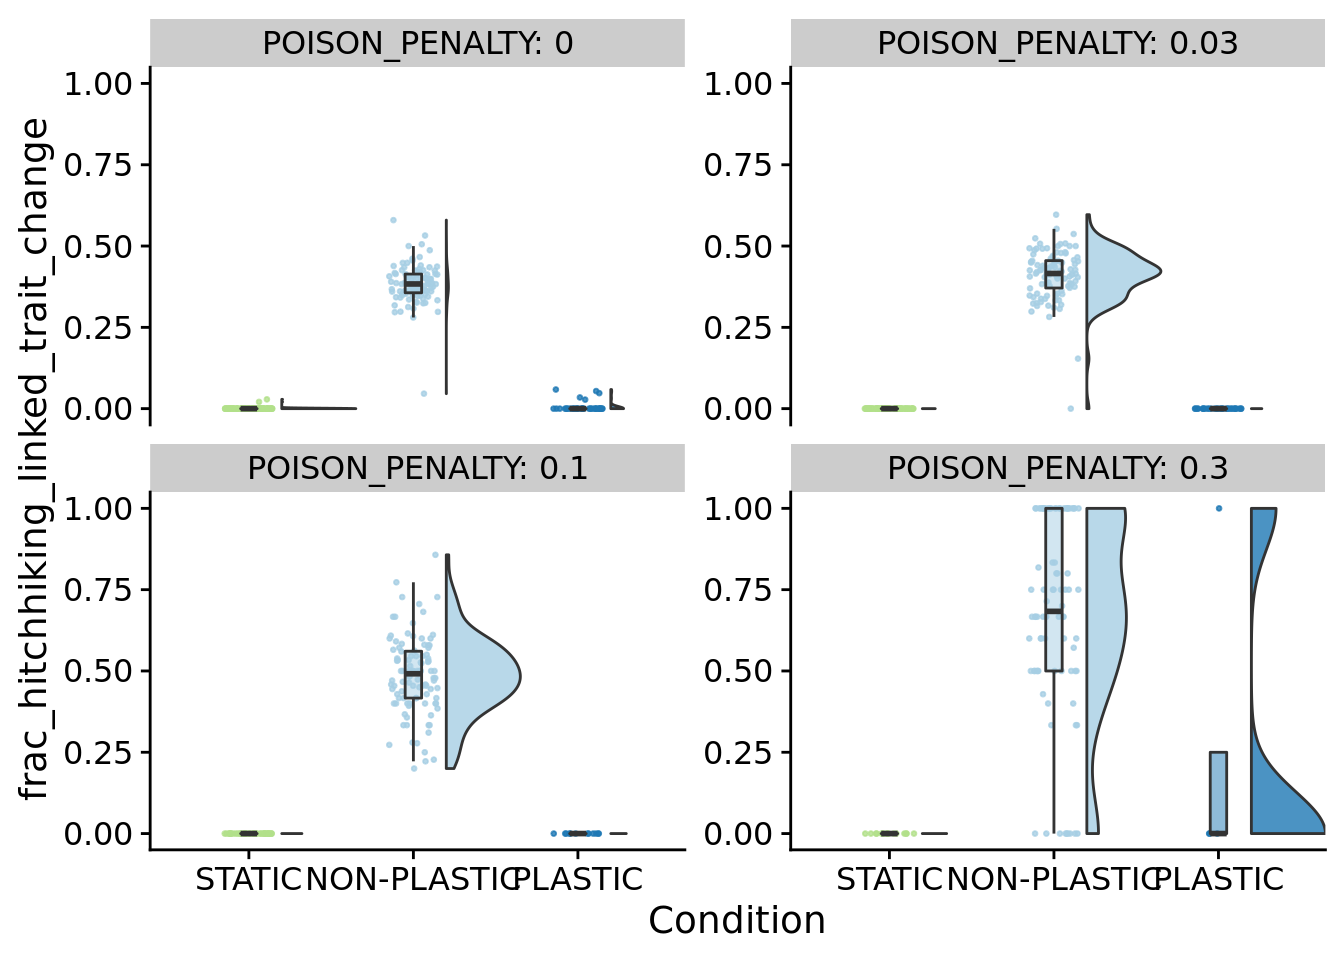
\includegraphics{supplemental-material_files/figure-latex/unnamed-chunk-83-1.pdf}

\hypertarget{frequency-of-increases-in-deleterious-instruction-execution-lineage}{%
\subsection{Frequency of increases in deleterious instruction execution (lineage)}\label{frequency-of-increases-in-deleterious-instruction-execution-lineage}}

\begin{Shaded}
\begin{Highlighting}[]
\KeywordTok{ggplot}\NormalTok{(summary_data, }\KeywordTok{aes}\NormalTok{(}\DataTypeTok{x=}\NormalTok{condition, }\DataTypeTok{y=}\NormalTok{dominant_lineage_num_times_hitchhike_inst_exec_increases_per_generation, }\DataTypeTok{fill=}\NormalTok{condition)) }\OperatorTok{+}
\StringTok{  }\KeywordTok{geom_flat_violin}\NormalTok{(}
    \DataTypeTok{position =} \KeywordTok{position_nudge}\NormalTok{(}\DataTypeTok{x =} \FloatTok{.2}\NormalTok{, }\DataTypeTok{y =} \DecValTok{0}\NormalTok{),}
    \DataTypeTok{alpha =} \FloatTok{.8}
\NormalTok{  ) }\OperatorTok{+}
\StringTok{  }\KeywordTok{geom_point}\NormalTok{(}
    \DataTypeTok{mapping=}\KeywordTok{aes}\NormalTok{(}\DataTypeTok{color=}\NormalTok{condition),}
    \DataTypeTok{position =} \KeywordTok{position_jitter}\NormalTok{(}\DataTypeTok{width =} \FloatTok{.15}\NormalTok{),}
    \DataTypeTok{size =} \FloatTok{.5}\NormalTok{,}
    \DataTypeTok{alpha =} \FloatTok{0.8}
\NormalTok{  ) }\OperatorTok{+}
\StringTok{  }\KeywordTok{geom_boxplot}\NormalTok{(}
    \DataTypeTok{width =} \FloatTok{.1}\NormalTok{,}
    \DataTypeTok{outlier.shape =} \OtherTok{NA}\NormalTok{,}
    \DataTypeTok{alpha =} \FloatTok{0.5}
\NormalTok{  ) }\OperatorTok{+}
\StringTok{  }\KeywordTok{scale_x_discrete}\NormalTok{(}
    \DataTypeTok{name=}\StringTok{"Condition"}\NormalTok{,}
    \DataTypeTok{limits=}\NormalTok{condition_order}
\NormalTok{  ) }\OperatorTok{+}
\StringTok{  }\KeywordTok{scale_fill_brewer}\NormalTok{(}
    \DataTypeTok{palette=}\NormalTok{cb_palette}
\NormalTok{  ) }\OperatorTok{+}
\StringTok{  }\KeywordTok{scale_color_brewer}\NormalTok{(}
    \DataTypeTok{palette=}\NormalTok{cb_palette}
\NormalTok{  ) }\OperatorTok{+}
\StringTok{  }\KeywordTok{facet_wrap}\NormalTok{(}
    \OperatorTok{~}\NormalTok{POISON_PENALTY,}
    \DataTypeTok{labeller=}\NormalTok{label_both,}
    \DataTypeTok{scales=}\StringTok{"free_y"}
\NormalTok{  ) }\OperatorTok{+}
\StringTok{  }\CommentTok{# coord_flip() +}
\StringTok{  }\KeywordTok{theme}\NormalTok{(}
    \DataTypeTok{legend.position=}\StringTok{"none"}
\NormalTok{  )}
\end{Highlighting}
\end{Shaded}

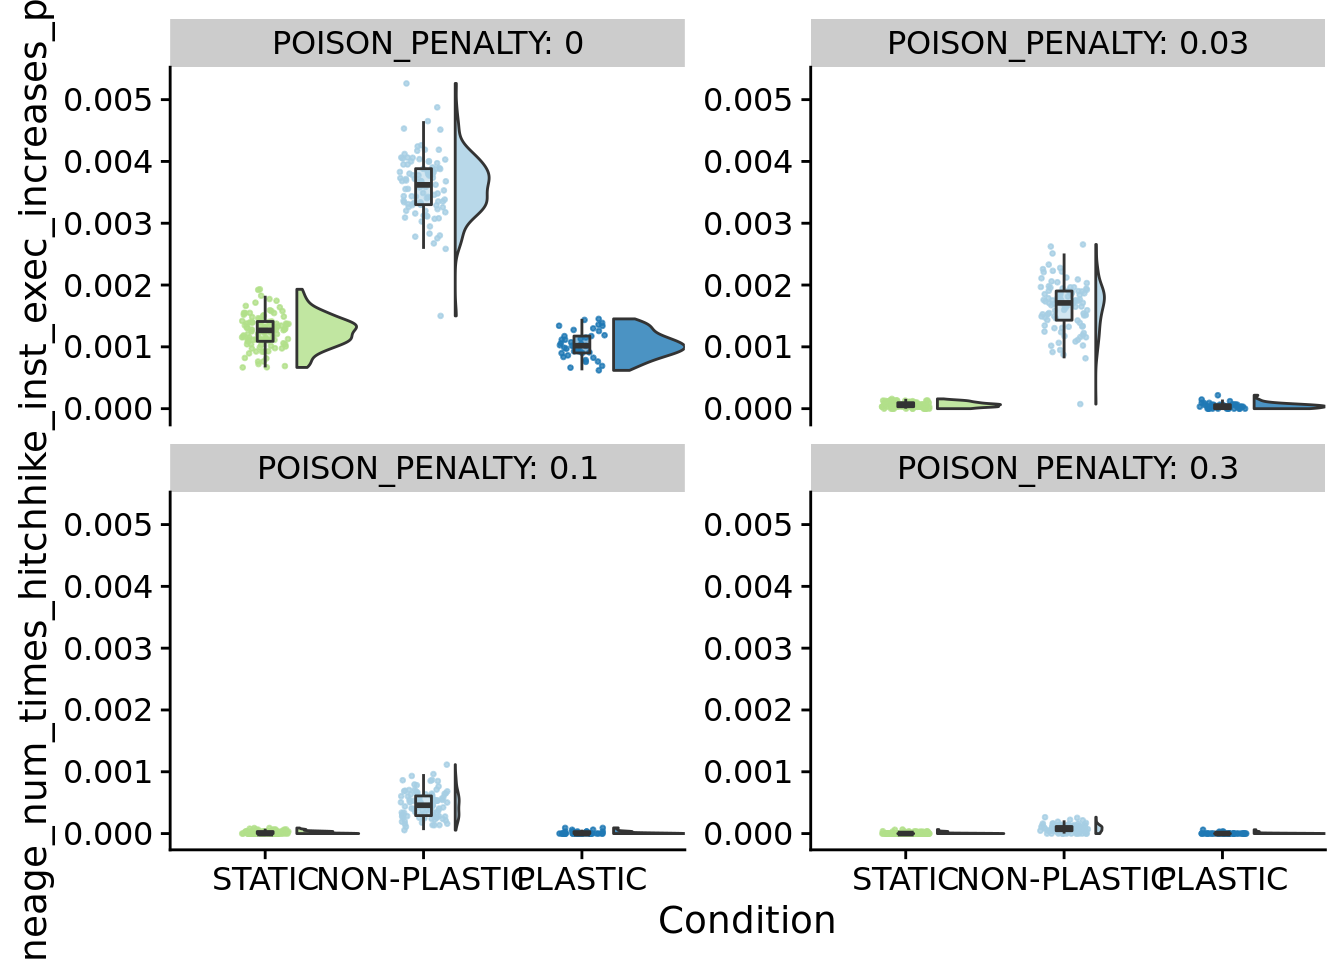
\includegraphics{supplemental-material_files/figure-latex/unnamed-chunk-84-1.pdf}

\begin{Shaded}
\begin{Highlighting}[]
\KeywordTok{ggsave}\NormalTok{(}
  \KeywordTok{paste0}\NormalTok{(working_directory, }\StringTok{"plots/final-dominant-lineage-poison-increase-per-generation.png"}\NormalTok{),}
  \DataTypeTok{width=}\DecValTok{15}\NormalTok{,}
  \DataTypeTok{height=}\DecValTok{10}
\NormalTok{)}
\end{Highlighting}
\end{Shaded}

\begin{Shaded}
\begin{Highlighting}[]
\ControlFlowTok{for}\NormalTok{ (penalty }\ControlFlowTok{in}\NormalTok{ poison_penalties) \{}
\NormalTok{  stat_data <-}\StringTok{ }\KeywordTok{filter}\NormalTok{(summary_data, POISON_PENALTY}\OperatorTok{==}\NormalTok{penalty)}
  \KeywordTok{print}\NormalTok{(}
    \KeywordTok{paste0}\NormalTok{(}
      \StringTok{"PENALTY: "}\NormalTok{, penalty}
\NormalTok{    )}
\NormalTok{  )}
\NormalTok{  kt <-}\StringTok{ }\KeywordTok{kruskal.test}\NormalTok{(}
      \DataTypeTok{formula=}\NormalTok{dominant_lineage_num_times_hitchhike_inst_exec_increases_per_generation}\OperatorTok{~}\NormalTok{condition,}
      \DataTypeTok{data=}\NormalTok{stat_data}
\NormalTok{    )}
  \KeywordTok{print}\NormalTok{(}
\NormalTok{    kt}
\NormalTok{  )}
  \ControlFlowTok{if}\NormalTok{ (}\KeywordTok{is.na}\NormalTok{(kt}\OperatorTok{$}\NormalTok{p.value)) \{ }\ControlFlowTok{next}\NormalTok{ \}}
  \ControlFlowTok{if}\NormalTok{ (kt}\OperatorTok{$}\NormalTok{p.value }\OperatorTok{>}\StringTok{ }\FloatTok{0.05}\NormalTok{) \{ }\ControlFlowTok{next}\NormalTok{ \}}
  \KeywordTok{print}\NormalTok{(}
    \KeywordTok{pairwise.wilcox.test}\NormalTok{(}
      \DataTypeTok{x=}\NormalTok{stat_data}\OperatorTok{$}\NormalTok{dominant_lineage_num_times_hitchhike_inst_exec_increases_per_generation,}
      \DataTypeTok{g=}\NormalTok{stat_data}\OperatorTok{$}\NormalTok{condition,}
      \DataTypeTok{p.adjust.method=}\StringTok{"bonferroni"}
\NormalTok{    )}
\NormalTok{  )}
\NormalTok{\}}
\end{Highlighting}
\end{Shaded}

\begin{verbatim}
## [1] "PENALTY: 0"
## 
##  Kruskal-Wallis rank sum test
## 
## data:  dominant_lineage_num_times_hitchhike_inst_exec_increases_per_generation by condition
## Kruskal-Wallis chi-squared = 180.05, df = 2, p-value < 2.2e-16
## 
## 
##  Pairwise comparisons using Wilcoxon rank sum test with continuity correction 
## 
## data:  stat_data$dominant_lineage_num_times_hitchhike_inst_exec_increases_per_generation and stat_data$condition 
## 
##         NON-PLASTIC PLASTIC
## PLASTIC < 2e-16     -      
## STATIC  < 2e-16     7.8e-05
## 
## P value adjustment method: bonferroni 
## [1] "PENALTY: 0.03"
## 
##  Kruskal-Wallis rank sum test
## 
## data:  dominant_lineage_num_times_hitchhike_inst_exec_increases_per_generation by condition
## Kruskal-Wallis chi-squared = 176.25, df = 2, p-value < 2.2e-16
## 
## 
##  Pairwise comparisons using Wilcoxon rank sum test with continuity correction 
## 
## data:  stat_data$dominant_lineage_num_times_hitchhike_inst_exec_increases_per_generation and stat_data$condition 
## 
##         NON-PLASTIC PLASTIC
## PLASTIC <2e-16      -      
## STATIC  <2e-16      0.019  
## 
## P value adjustment method: bonferroni 
## [1] "PENALTY: 0.1"
## 
##  Kruskal-Wallis rank sum test
## 
## data:  dominant_lineage_num_times_hitchhike_inst_exec_increases_per_generation by condition
## Kruskal-Wallis chi-squared = 184.17, df = 2, p-value < 2.2e-16
## 
## 
##  Pairwise comparisons using Wilcoxon rank sum test with continuity correction 
## 
## data:  stat_data$dominant_lineage_num_times_hitchhike_inst_exec_increases_per_generation and stat_data$condition 
## 
##         NON-PLASTIC PLASTIC
## PLASTIC <2e-16      -      
## STATIC  <2e-16      0.2    
## 
## P value adjustment method: bonferroni 
## [1] "PENALTY: 0.3"
## 
##  Kruskal-Wallis rank sum test
## 
## data:  dominant_lineage_num_times_hitchhike_inst_exec_increases_per_generation by condition
## Kruskal-Wallis chi-squared = 140.99, df = 2, p-value < 2.2e-16
## 
## 
##  Pairwise comparisons using Wilcoxon rank sum test with continuity correction 
## 
## data:  stat_data$dominant_lineage_num_times_hitchhike_inst_exec_increases_per_generation and stat_data$condition 
## 
##         NON-PLASTIC PLASTIC
## PLASTIC 2.2e-15     -      
## STATIC  < 2e-16     0.79   
## 
## P value adjustment method: bonferroni
\end{verbatim}

Figure for the manuscript:

\begin{Shaded}
\begin{Highlighting}[]
\CommentTok{# Compute manual labels for geom_signif}
\NormalTok{stat.test <-}\StringTok{ }\NormalTok{focal_summary_data }\OperatorTok
\StringTok{  }\KeywordTok{wilcox_test}\NormalTok{(dominant_lineage_num_times_hitchhike_inst_exec_increases_per_generation }\OperatorTok{~}\StringTok{ }\NormalTok{condition) }\OperatorTok
\StringTok{  }\KeywordTok{adjust_pvalue}\NormalTok{(}\DataTypeTok{method =} \StringTok{"bonferroni"}\NormalTok{) }\OperatorTok
\StringTok{  }\KeywordTok{add_significance}\NormalTok{() }\OperatorTok
\StringTok{  }\KeywordTok{add_xy_position}\NormalTok{(}\DataTypeTok{x=}\StringTok{"condition"}\NormalTok{, }\DataTypeTok{step.increase=}\FloatTok{0.2}\NormalTok{)}
\CommentTok{# Tweak y.position manually to account for scaled axis (edge case that triggers bad behavior in geom_signif)}
\NormalTok{stat.test}\OperatorTok{$}\NormalTok{manual_position <-}\StringTok{  }\NormalTok{stat.test}\OperatorTok{$}\NormalTok{y.position}
\NormalTok{stat.test}\OperatorTok{$}\NormalTok{label <-}\StringTok{ }\KeywordTok{mapply}\NormalTok{(p_label,stat.test}\OperatorTok{$}\NormalTok{p.adj)}

\NormalTok{poison_increases_per_gen_fig <-}\StringTok{ }\KeywordTok{ggplot}\NormalTok{(}
\NormalTok{    focal_summary_data,}
    \KeywordTok{aes}\NormalTok{(}\DataTypeTok{x=}\NormalTok{condition, }\DataTypeTok{y=}\NormalTok{dominant_lineage_num_times_hitchhike_inst_exec_increases_per_generation, }\DataTypeTok{fill=}\NormalTok{condition)}
\NormalTok{  ) }\OperatorTok{+}
\StringTok{  }\KeywordTok{geom_flat_violin}\NormalTok{(}
    \DataTypeTok{scale=}\StringTok{"width"}\NormalTok{,}
    \DataTypeTok{position =} \KeywordTok{position_nudge}\NormalTok{(}\DataTypeTok{x =} \FloatTok{.2}\NormalTok{, }\DataTypeTok{y =} \DecValTok{0}\NormalTok{),}
    \DataTypeTok{alpha =} \FloatTok{.8}
\NormalTok{  ) }\OperatorTok{+}
\StringTok{  }\KeywordTok{geom_point}\NormalTok{(}
    \DataTypeTok{mapping=}\KeywordTok{aes}\NormalTok{(}\DataTypeTok{color=}\NormalTok{condition),}
    \DataTypeTok{position =} \KeywordTok{position_jitter}\NormalTok{(}\DataTypeTok{width =} \FloatTok{.15}\NormalTok{),}
    \DataTypeTok{size =} \FloatTok{.5}\NormalTok{,}
    \DataTypeTok{alpha =} \FloatTok{0.8}
\NormalTok{  ) }\OperatorTok{+}
\StringTok{  }\KeywordTok{geom_boxplot}\NormalTok{(}
    \DataTypeTok{width =} \FloatTok{.1}\NormalTok{,}
    \DataTypeTok{outlier.shape =} \OtherTok{NA}\NormalTok{,}
    \DataTypeTok{alpha =} \FloatTok{0.5}
\NormalTok{  ) }\OperatorTok{+}
\StringTok{  }\KeywordTok{scale_x_discrete}\NormalTok{(}
    \DataTypeTok{name=}\StringTok{"Condition"}\NormalTok{,}
    \DataTypeTok{limits=}\NormalTok{condition_order,}
    \DataTypeTok{labels=}\NormalTok{condition_order}
\NormalTok{  ) }\OperatorTok{+}
\StringTok{  }\KeywordTok{scale_y_continuous}\NormalTok{(}
    \DataTypeTok{name=}\StringTok{"Deleterious function acquisition frequency"}\NormalTok{,}
\NormalTok{  ) }\OperatorTok{+}
\StringTok{  }\KeywordTok{scale_fill_brewer}\NormalTok{(}
    \DataTypeTok{palette=}\NormalTok{cb_palette}
\NormalTok{  ) }\OperatorTok{+}
\StringTok{  }\KeywordTok{scale_color_brewer}\NormalTok{(}
    \DataTypeTok{palette=}\NormalTok{cb_palette}
\NormalTok{  ) }\OperatorTok{+}
\StringTok{  }\CommentTok{# coord_flip()}
\StringTok{  }\KeywordTok{labs}\NormalTok{(}
    \DataTypeTok{subtitle=}\KeywordTok{paste0}\NormalTok{(}
      \StringTok{"Kruskal-Wallis, "}\NormalTok{,}
      \KeywordTok{p_label}\NormalTok{(}\KeywordTok{signif}\NormalTok{(}\KeywordTok{kruskal.test}\NormalTok{(}\DataTypeTok{formula=}\NormalTok{dominant_lineage_num_times_hitchhike_inst_exec_increases_per_generation}\OperatorTok{~}\NormalTok{condition, }\DataTypeTok{data=}\NormalTok{focal_summary_data)}\OperatorTok{$}\NormalTok{p.value,}\DataTypeTok{digits=}\DecValTok{4}\NormalTok{))}
\NormalTok{    )}
\NormalTok{  ) }\OperatorTok{+}
\StringTok{  }\NormalTok{ggsignif}\OperatorTok{::}\KeywordTok{geom_signif}\NormalTok{(}
    \DataTypeTok{data=}\KeywordTok{filter}\NormalTok{(stat.test, p.adj }\OperatorTok{<=}\StringTok{ }\NormalTok{alpha),}
    \KeywordTok{aes}\NormalTok{(}\DataTypeTok{xmin=}\NormalTok{group1,}\DataTypeTok{xmax=}\NormalTok{group2,}\DataTypeTok{annotations=}\NormalTok{label,}\DataTypeTok{y_position=}\NormalTok{manual_position),}
    \DataTypeTok{manual=}\OtherTok{TRUE}\NormalTok{,}
    \DataTypeTok{inherit.aes=}\OtherTok{FALSE}
\NormalTok{  ) }\OperatorTok{+}
\StringTok{  }\KeywordTok{theme}\NormalTok{(}
    \DataTypeTok{legend.position=}\StringTok{"none"}
\NormalTok{  )}
\end{Highlighting}
\end{Shaded}

\begin{verbatim}
## Warning: Ignoring unknown aesthetics: xmin, xmax, annotations, y_position
\end{verbatim}

\begin{Shaded}
\begin{Highlighting}[]
\NormalTok{poison_increases_per_gen_fig}
\end{Highlighting}
\end{Shaded}

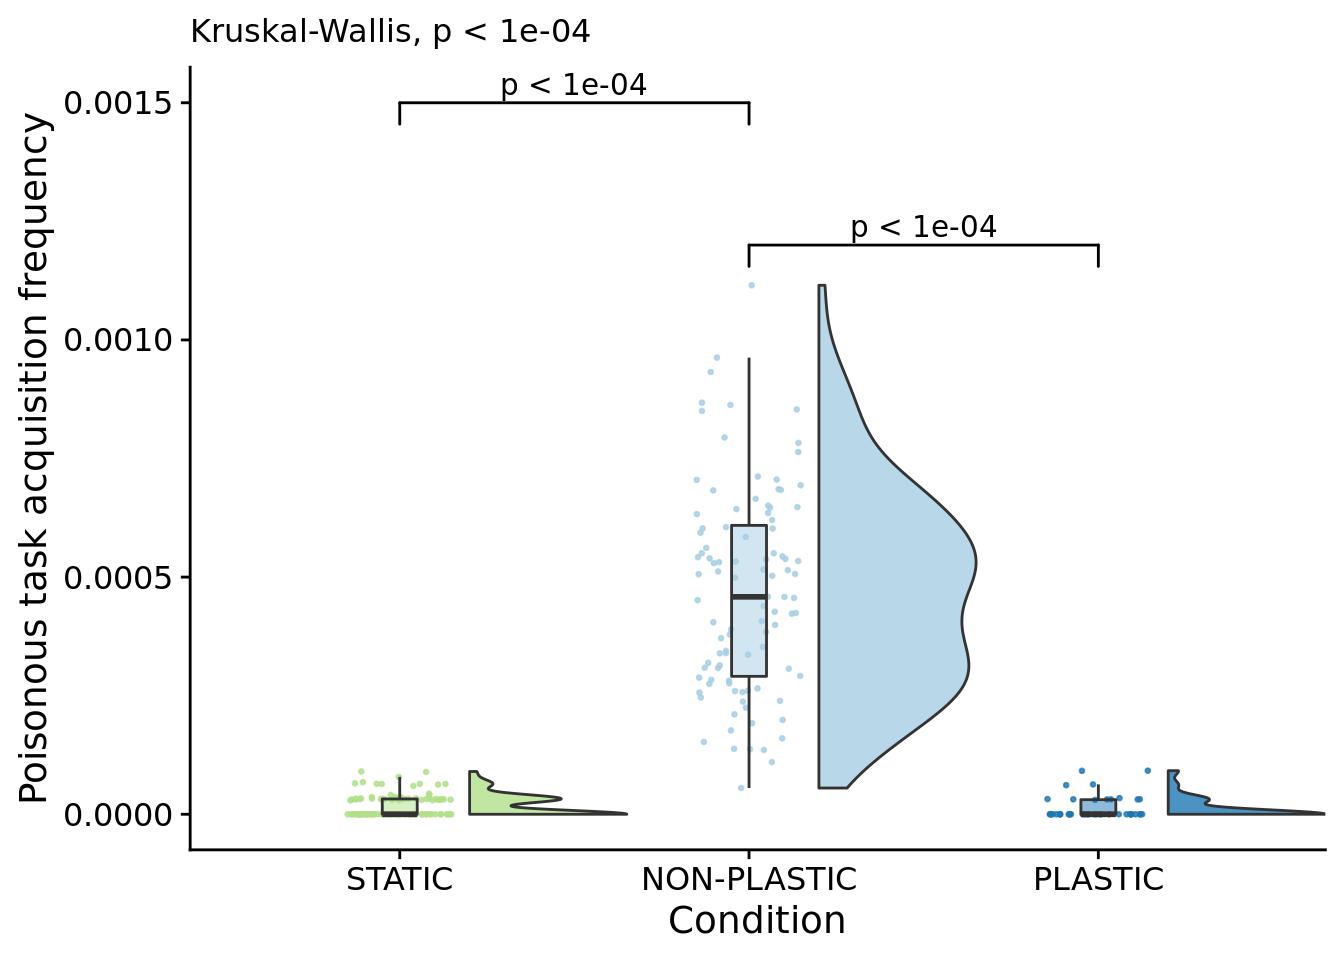
\includegraphics{supplemental-material_files/figure-latex/unnamed-chunk-86-1.pdf}

\hypertarget{what-fraction-of-mutations-that-increase-deleterious-instruction-execution-co-occur-with-base-trait-changes}{%
\subsection{What fraction of mutations that increase deleterious instruction execution co-occur with base trait changes?}\label{what-fraction-of-mutations-that-increase-deleterious-instruction-execution-co-occur-with-base-trait-changes}}

\begin{Shaded}
\begin{Highlighting}[]
\KeywordTok{ggplot}\NormalTok{(}\KeywordTok{filter}\NormalTok{(summary_data, dominant_lineage_num_times_hitchhike_inst_exec_increases}\OperatorTok{>}\DecValTok{0}\NormalTok{), }\KeywordTok{aes}\NormalTok{(}\DataTypeTok{x=}\NormalTok{frac_hitchhiking_linked_trait_change, }\DataTypeTok{fill=}\NormalTok{condition)) }\OperatorTok{+}
\StringTok{  }\KeywordTok{geom_density}\NormalTok{() }\OperatorTok{+}
\StringTok{  }\KeywordTok{facet_grid}\NormalTok{(}
\NormalTok{    condition}\OperatorTok{~}\NormalTok{POISON_PENALTY,}
    \DataTypeTok{labeller=}\NormalTok{label_both,}
    \DataTypeTok{scales=}\StringTok{"free_y"}
\NormalTok{  ) }\OperatorTok{+}
\StringTok{  }\KeywordTok{scale_fill_brewer}\NormalTok{(}
    \DataTypeTok{palette=}\NormalTok{cb_palette}
\NormalTok{  ) }\OperatorTok{+}
\StringTok{  }\KeywordTok{scale_color_brewer}\NormalTok{(}
    \DataTypeTok{palette=}\NormalTok{cb_palette}
\NormalTok{  ) }\OperatorTok{+}
\StringTok{  }\KeywordTok{theme}\NormalTok{(}
    \DataTypeTok{legend.position=}\StringTok{"none"}
\NormalTok{  )}
\end{Highlighting}
\end{Shaded}

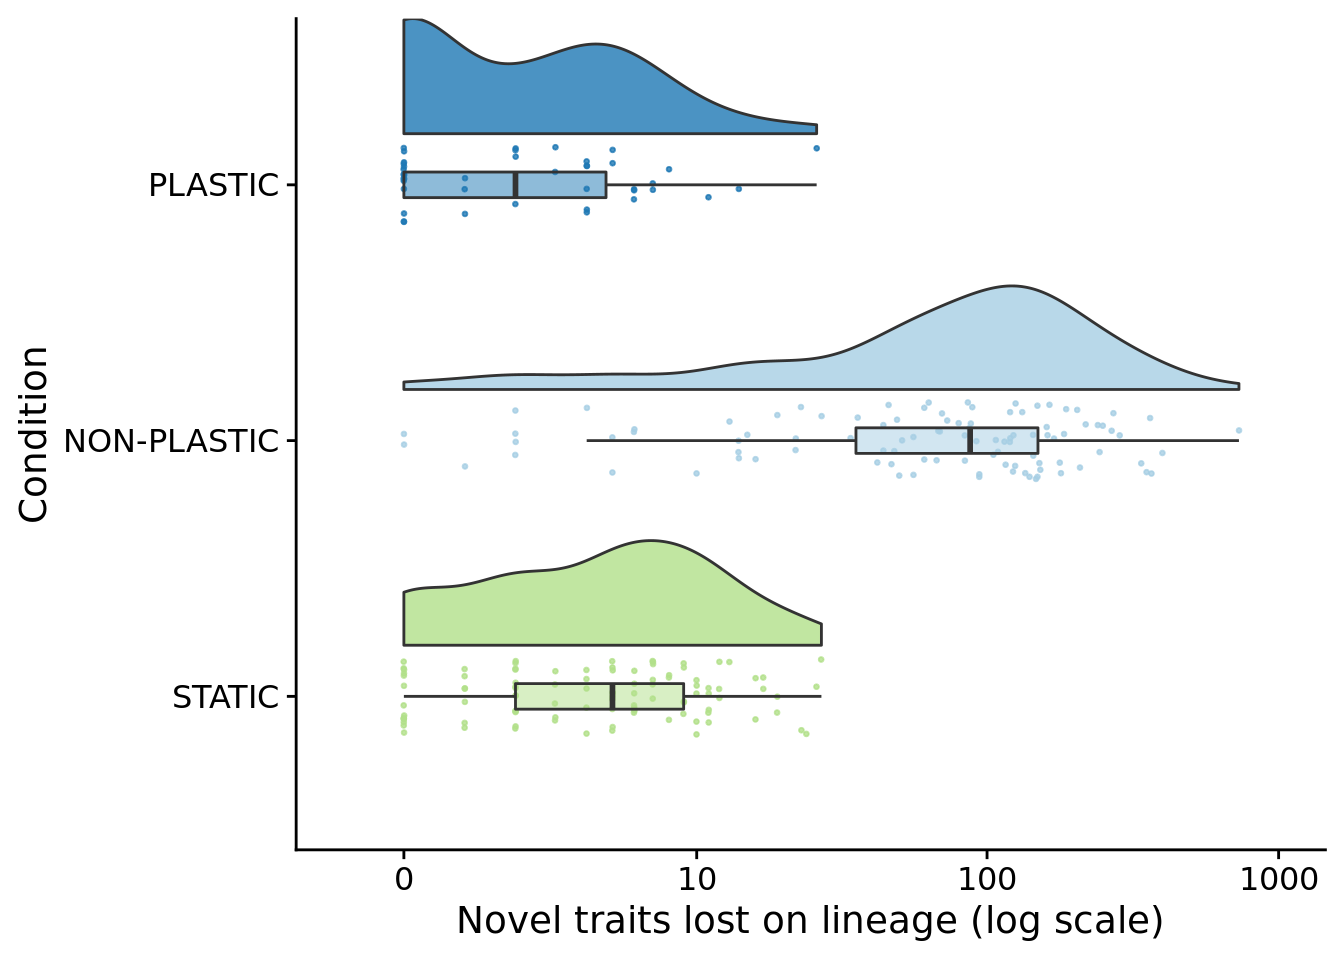
\includegraphics{supplemental-material_files/figure-latex/unnamed-chunk-87-1.pdf}

\begin{Shaded}
\begin{Highlighting}[]
\KeywordTok{ggsave}\NormalTok{(}
  \KeywordTok{paste0}\NormalTok{(working_directory, }\StringTok{"plots/dominant-lineage-frac_hitchhiking_linked_trait_change.png"}\NormalTok{),}
  \DataTypeTok{width=}\DecValTok{15}\NormalTok{,}
  \DataTypeTok{height=}\DecValTok{10}
\NormalTok{)}
\end{Highlighting}
\end{Shaded}

\begin{Shaded}
\begin{Highlighting}[]
\KeywordTok{ggplot}\NormalTok{(}\KeywordTok{filter}\NormalTok{(summary_data, dominant_lineage_num_times_hitchhike_inst_exec_increases}\OperatorTok{>}\DecValTok{0}\NormalTok{ ), }\KeywordTok{aes}\NormalTok{(}\DataTypeTok{x=}\NormalTok{condition, }\DataTypeTok{y=}\NormalTok{frac_hitchhiking_linked_trait_change, }\DataTypeTok{fill=}\NormalTok{condition)) }\OperatorTok{+}
\StringTok{  }\KeywordTok{geom_flat_violin}\NormalTok{(}
    \DataTypeTok{position =} \KeywordTok{position_nudge}\NormalTok{(}\DataTypeTok{x =} \FloatTok{.2}\NormalTok{, }\DataTypeTok{y =} \DecValTok{0}\NormalTok{),}
    \DataTypeTok{alpha =} \FloatTok{.8}
\NormalTok{  ) }\OperatorTok{+}
\StringTok{  }\KeywordTok{geom_point}\NormalTok{(}
    \DataTypeTok{mapping=}\KeywordTok{aes}\NormalTok{(}\DataTypeTok{color=}\NormalTok{condition),}
    \DataTypeTok{position =} \KeywordTok{position_jitter}\NormalTok{(}\DataTypeTok{width =} \FloatTok{.15}\NormalTok{),}
    \DataTypeTok{size =} \FloatTok{.5}\NormalTok{,}
    \DataTypeTok{alpha =} \FloatTok{0.8}
\NormalTok{  ) }\OperatorTok{+}
\StringTok{  }\KeywordTok{geom_boxplot}\NormalTok{(}
    \DataTypeTok{width =} \FloatTok{.1}\NormalTok{,}
    \DataTypeTok{outlier.shape =} \OtherTok{NA}\NormalTok{,}
    \DataTypeTok{alpha =} \FloatTok{0.5}
\NormalTok{  ) }\OperatorTok{+}
\StringTok{  }\KeywordTok{scale_x_discrete}\NormalTok{(}
    \DataTypeTok{name=}\StringTok{"Condition"}\NormalTok{,}
    \DataTypeTok{limits=}\NormalTok{condition_order}
\NormalTok{  ) }\OperatorTok{+}
\StringTok{  }\KeywordTok{scale_fill_brewer}\NormalTok{(}
    \DataTypeTok{palette=}\NormalTok{cb_palette}
\NormalTok{  ) }\OperatorTok{+}
\StringTok{  }\KeywordTok{scale_color_brewer}\NormalTok{(}
    \DataTypeTok{palette=}\NormalTok{cb_palette}
\NormalTok{  ) }\OperatorTok{+}
\StringTok{  }\KeywordTok{facet_wrap}\NormalTok{(}
    \OperatorTok{~}\NormalTok{POISON_PENALTY,}
    \DataTypeTok{labeller=}\NormalTok{label_both,}
    \DataTypeTok{scales=}\StringTok{"free_y"}
\NormalTok{  ) }\OperatorTok{+}
\StringTok{  }\CommentTok{# coord_flip() +}
\StringTok{  }\KeywordTok{theme}\NormalTok{(}
    \DataTypeTok{legend.position=}\StringTok{"none"}
\NormalTok{  )}
\end{Highlighting}
\end{Shaded}

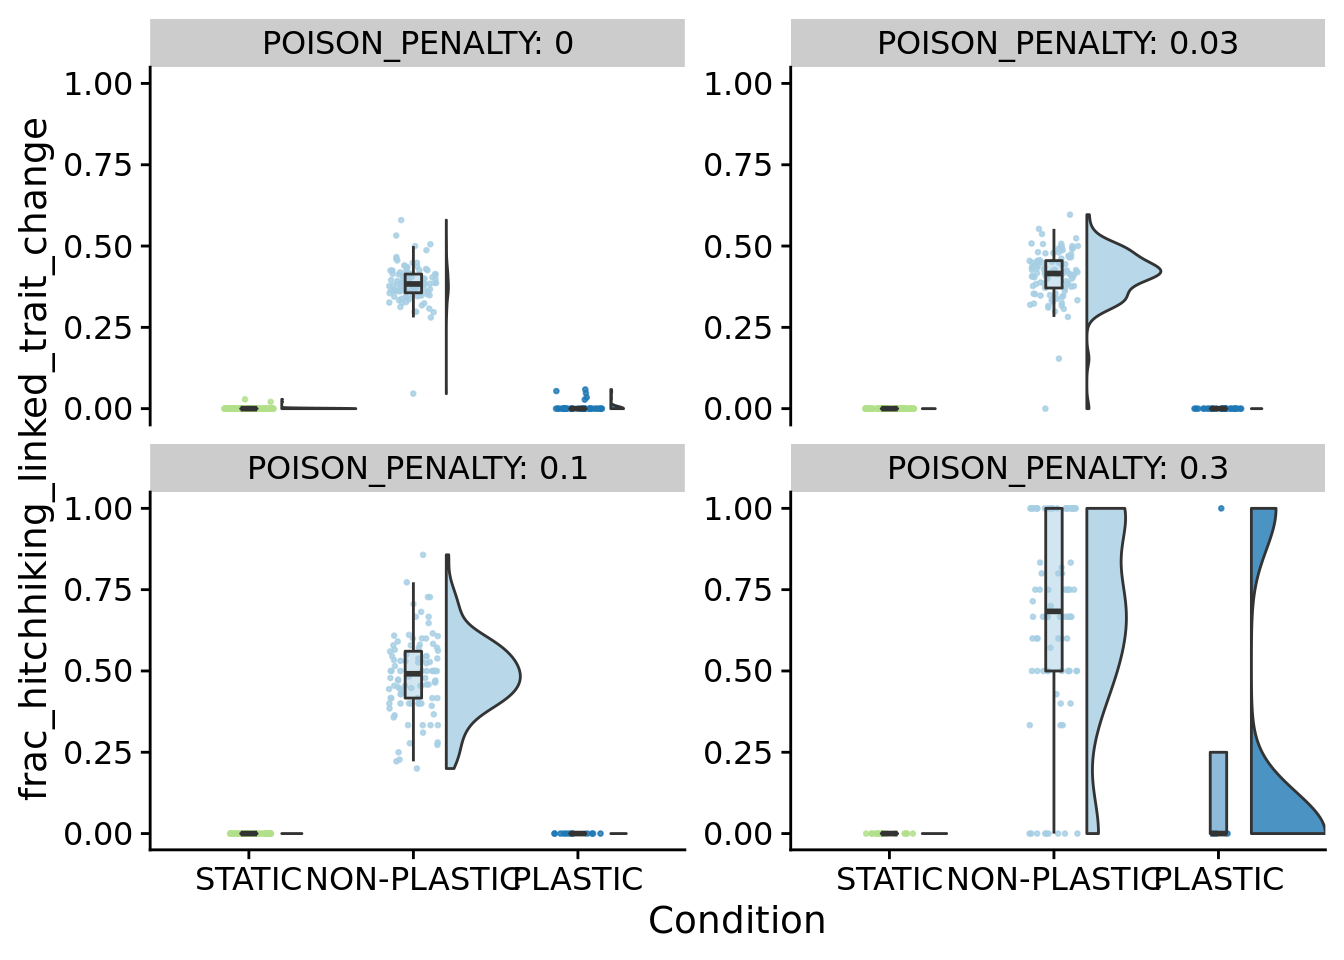
\includegraphics{supplemental-material_files/figure-latex/unnamed-chunk-88-1.pdf}

\begin{Shaded}
\begin{Highlighting}[]
\ControlFlowTok{for}\NormalTok{ (penalty }\ControlFlowTok{in}\NormalTok{ poison_penalties) \{}
\NormalTok{  stat_data <-}\StringTok{ }\KeywordTok{filter}\NormalTok{(summary_data, POISON_PENALTY}\OperatorTok{==}\NormalTok{penalty }\OperatorTok{&}\StringTok{ }\NormalTok{dominant_lineage_num_times_hitchhike_inst_exec_increases}\OperatorTok{>}\DecValTok{0}\NormalTok{)}
  \KeywordTok{print}\NormalTok{(}
    \KeywordTok{paste0}\NormalTok{(}
      \StringTok{"PENALTY: "}\NormalTok{, penalty}
\NormalTok{    )}
\NormalTok{  )}
\NormalTok{  kt <-}\StringTok{ }\KeywordTok{kruskal.test}\NormalTok{(}
      \DataTypeTok{formula=}\NormalTok{frac_hitchhiking_linked_trait_change}\OperatorTok{~}\NormalTok{condition,}
      \DataTypeTok{data=}\NormalTok{stat_data}
\NormalTok{    )}
  \KeywordTok{print}\NormalTok{(}
\NormalTok{    kt}
\NormalTok{  )}
  \ControlFlowTok{if}\NormalTok{ (}\KeywordTok{is.na}\NormalTok{(kt}\OperatorTok{$}\NormalTok{p.value)) \{ }\ControlFlowTok{next}\NormalTok{ \}}
  \ControlFlowTok{if}\NormalTok{ (kt}\OperatorTok{$}\NormalTok{p.value }\OperatorTok{>}\StringTok{ }\FloatTok{0.05}\NormalTok{) \{ }\ControlFlowTok{next}\NormalTok{ \}}
  \KeywordTok{print}\NormalTok{(}
    \KeywordTok{pairwise.wilcox.test}\NormalTok{(}
      \DataTypeTok{x=}\NormalTok{stat_data}\OperatorTok{$}\NormalTok{frac_hitchhiking_linked_trait_change,}
      \DataTypeTok{g=}\NormalTok{stat_data}\OperatorTok{$}\NormalTok{condition,}
      \DataTypeTok{p.adjust.method=}\StringTok{"bonferroni"}\NormalTok{,}
      \DataTypeTok{exact=}\OtherTok{FALSE}
\NormalTok{    )}
\NormalTok{  )}
\NormalTok{\}}
\end{Highlighting}
\end{Shaded}

\begin{verbatim}
## [1] "PENALTY: 0"
## 
##  Kruskal-Wallis rank sum test
## 
## data:  frac_hitchhiking_linked_trait_change by condition
## Kruskal-Wallis chi-squared = 211.29, df = 2, p-value < 2.2e-16
## 
## 
##  Pairwise comparisons using Wilcoxon rank sum test with continuity correction 
## 
## data:  stat_data$frac_hitchhiking_linked_trait_change and stat_data$condition 
## 
##         NON-PLASTIC PLASTIC
## PLASTIC <2e-16      -      
## STATIC  <2e-16      0.031  
## 
## P value adjustment method: bonferroni 
## [1] "PENALTY: 0.03"
## 
##  Kruskal-Wallis rank sum test
## 
## data:  frac_hitchhiking_linked_trait_change by condition
## Kruskal-Wallis chi-squared = 186.88, df = 2, p-value < 2.2e-16
## 
## 
##  Pairwise comparisons using Wilcoxon rank sum test with continuity correction 
## 
## data:  stat_data$frac_hitchhiking_linked_trait_change and stat_data$condition 
## 
##         NON-PLASTIC PLASTIC
## PLASTIC 2.9e-16     -      
## STATIC  < 2e-16     -      
## 
## P value adjustment method: bonferroni 
## [1] "PENALTY: 0.1"
## 
##  Kruskal-Wallis rank sum test
## 
## data:  frac_hitchhiking_linked_trait_change by condition
## Kruskal-Wallis chi-squared = 113.72, df = 2, p-value < 2.2e-16
## 
## 
##  Pairwise comparisons using Wilcoxon rank sum test with continuity correction 
## 
## data:  stat_data$frac_hitchhiking_linked_trait_change and stat_data$condition 
## 
##         NON-PLASTIC PLASTIC
## PLASTIC 3.3e-08     -      
## STATIC  < 2e-16     -      
## 
## P value adjustment method: bonferroni 
## [1] "PENALTY: 0.3"
## 
##  Kruskal-Wallis rank sum test
## 
## data:  frac_hitchhiking_linked_trait_change by condition
## Kruskal-Wallis chi-squared = 34.791, df = 2, p-value = 2.788e-08
## 
## 
##  Pairwise comparisons using Wilcoxon rank sum test with continuity correction 
## 
## data:  stat_data$frac_hitchhiking_linked_trait_change and stat_data$condition 
## 
##         NON-PLASTIC PLASTIC
## PLASTIC 0.26        -      
## STATIC  2.4e-08     0.18   
## 
## P value adjustment method: bonferroni
\end{verbatim}

\begin{Shaded}
\begin{Highlighting}[]
\NormalTok{denom <-}\StringTok{ }\KeywordTok{sum}\NormalTok{(}\KeywordTok{filter}\NormalTok{(summary_data, condition}\OperatorTok{==}\StringTok{"NON-PLASTIC"} \OperatorTok{&}\StringTok{ }\NormalTok{POISON_PENALTY}\OperatorTok{==}\FloatTok{0.1}\NormalTok{)}\OperatorTok{$}\NormalTok{dominant_lineage_num_times_hitchhike_inst_exec_increases)}
\NormalTok{num <-}\StringTok{ }\KeywordTok{sum}\NormalTok{(}\KeywordTok{filter}\NormalTok{(summary_data, condition}\OperatorTok{==}\StringTok{"NON-PLASTIC"} \OperatorTok{&}\StringTok{ }\NormalTok{POISON_PENALTY}\OperatorTok{==}\FloatTok{0.1}\NormalTok{)}\OperatorTok{$}\NormalTok{dominant_lineage_num_times_hitchhike_inst_exec_increases_with_primary_trait_change)}
\KeywordTok{paste0}\NormalTok{(}\StringTok{"NON-PLASTIC (0.1 penalty): "}\NormalTok{, num}\OperatorTok{/}\NormalTok{denom, }\StringTok{"("}\NormalTok{, num, }\StringTok{"/"}\NormalTok{, denom, }\StringTok{")"}\NormalTok{)}
\end{Highlighting}
\end{Shaded}

\begin{verbatim}
## [1] "NON-PLASTIC (0.1 penalty): 0.498956158663883(956/1916)"
\end{verbatim}

\begin{Shaded}
\begin{Highlighting}[]
\NormalTok{denom <-}\StringTok{ }\KeywordTok{sum}\NormalTok{(}\KeywordTok{filter}\NormalTok{(summary_data, condition}\OperatorTok{==}\StringTok{"PLASTIC"} \OperatorTok{&}\StringTok{ }\NormalTok{POISON_PENALTY}\OperatorTok{==}\FloatTok{0.1}\NormalTok{)}\OperatorTok{$}\NormalTok{dominant_lineage_num_times_hitchhike_inst_exec_increases)}
\NormalTok{num <-}\StringTok{ }\KeywordTok{sum}\NormalTok{(}\KeywordTok{filter}\NormalTok{(summary_data, condition}\OperatorTok{==}\StringTok{"PLASTIC"} \OperatorTok{&}\StringTok{ }\NormalTok{POISON_PENALTY}\OperatorTok{==}\FloatTok{0.1}\NormalTok{)}\OperatorTok{$}\NormalTok{dominant_lineage_num_times_hitchhike_inst_exec_increases_with_primary_trait_change)}
\KeywordTok{paste0}\NormalTok{(}\StringTok{"PLASTIC (0.1 penalty): "}\NormalTok{, num}\OperatorTok{/}\NormalTok{denom, }\StringTok{" ("}\NormalTok{, num, }\StringTok{"/"}\NormalTok{, denom, }\StringTok{")"}\NormalTok{)}
\end{Highlighting}
\end{Shaded}

\begin{verbatim}
## [1] "PLASTIC (0.1 penalty): 0 (0/18)"
\end{verbatim}

\begin{Shaded}
\begin{Highlighting}[]
\NormalTok{denom <-}\StringTok{ }\KeywordTok{sum}\NormalTok{(}\KeywordTok{filter}\NormalTok{(summary_data, condition}\OperatorTok{==}\StringTok{"STATIC"} \OperatorTok{&}\StringTok{ }\NormalTok{POISON_PENALTY}\OperatorTok{==}\FloatTok{0.1}\NormalTok{)}\OperatorTok{$}\NormalTok{dominant_lineage_num_times_hitchhike_inst_exec_increases)}
\NormalTok{num <-}\StringTok{ }\KeywordTok{sum}\NormalTok{(}\KeywordTok{filter}\NormalTok{(summary_data, condition}\OperatorTok{==}\StringTok{"STATIC"} \OperatorTok{&}\StringTok{ }\NormalTok{POISON_PENALTY}\OperatorTok{==}\FloatTok{0.1}\NormalTok{)}\OperatorTok{$}\NormalTok{dominant_lineage_num_times_hitchhike_inst_exec_increases_with_primary_trait_change)}
\KeywordTok{paste0}\NormalTok{(}\StringTok{"STATIC (0.1 penalty): "}\NormalTok{, num}\OperatorTok{/}\NormalTok{denom, }\StringTok{" ("}\NormalTok{, num, }\StringTok{"/"}\NormalTok{, denom, }\StringTok{")"}\NormalTok{)}
\end{Highlighting}
\end{Shaded}

\begin{verbatim}
## [1] "STATIC (0.1 penalty): 0 (0/58)"
\end{verbatim}

Focal figure for the manuscript:

\begin{Shaded}
\begin{Highlighting}[]
\CommentTok{# Compute manual labels for geom_signif}
\NormalTok{stat.test <-}\KeywordTok{filter}\NormalTok{(focal_summary_data,dominant_lineage_num_times_hitchhike_inst_exec_increases}\OperatorTok{>}\DecValTok{0}\NormalTok{) }\OperatorTok
\StringTok{  }\KeywordTok{wilcox_test}\NormalTok{(frac_hitchhiking_linked_trait_change }\OperatorTok{~}\StringTok{ }\NormalTok{condition, }\DataTypeTok{comparisons=}\KeywordTok{list}\NormalTok{(}\KeywordTok{c}\NormalTok{(}\StringTok{"PLASTIC"}\NormalTok{, }\StringTok{"NON-PLASTIC"}\NormalTok{), }\KeywordTok{c}\NormalTok{(}\StringTok{"STATIC"}\NormalTok{, }\StringTok{"NON-PLASTIC"}\NormalTok{))) }\OperatorTok
\StringTok{  }\KeywordTok{adjust_pvalue}\NormalTok{(}\DataTypeTok{method =} \StringTok{"bonferroni"}\NormalTok{) }\OperatorTok
\StringTok{  }\KeywordTok{add_significance}\NormalTok{() }\OperatorTok
\StringTok{  }\KeywordTok{add_xy_position}\NormalTok{(}\DataTypeTok{x=}\StringTok{"condition"}\NormalTok{)}
\CommentTok{# Tweak y.position manually to account for scaled axis (edge case that triggers bad behavior in geom_signif)}
\NormalTok{stat.test}\OperatorTok{$}\NormalTok{manual_position <-}\StringTok{  }\NormalTok{stat.test}\OperatorTok{$}\NormalTok{y.position}
\NormalTok{stat.test}\OperatorTok{$}\NormalTok{label <-}\StringTok{ }\KeywordTok{mapply}\NormalTok{(p_label,stat.test}\OperatorTok{$}\NormalTok{p.adj)}

\NormalTok{linked_trait_change_fig <-}\StringTok{ }\KeywordTok{ggplot}\NormalTok{(}
    \KeywordTok{filter}\NormalTok{(focal_summary_data, dominant_lineage_num_times_hitchhike_inst_exec_increases}\OperatorTok{>}\DecValTok{0}\NormalTok{),}
    \KeywordTok{aes}\NormalTok{(}\DataTypeTok{x=}\NormalTok{condition, }\DataTypeTok{y=}\NormalTok{frac_hitchhiking_linked_trait_change, }\DataTypeTok{fill=}\NormalTok{condition)}
\NormalTok{  ) }\OperatorTok{+}
\StringTok{  }\KeywordTok{geom_flat_violin}\NormalTok{(}
    \DataTypeTok{scale=}\StringTok{"width"}\NormalTok{,}
    \DataTypeTok{position =} \KeywordTok{position_nudge}\NormalTok{(}\DataTypeTok{x =} \FloatTok{.2}\NormalTok{, }\DataTypeTok{y =} \DecValTok{0}\NormalTok{),}
    \DataTypeTok{alpha =} \FloatTok{.8}
\NormalTok{  ) }\OperatorTok{+}
\StringTok{  }\KeywordTok{geom_point}\NormalTok{(}
    \DataTypeTok{mapping=}\KeywordTok{aes}\NormalTok{(}\DataTypeTok{color=}\NormalTok{condition),}
    \DataTypeTok{position =} \KeywordTok{position_jitter}\NormalTok{(}\DataTypeTok{width =} \FloatTok{.15}\NormalTok{),}
    \DataTypeTok{size =} \FloatTok{.5}\NormalTok{,}
    \DataTypeTok{alpha =} \FloatTok{0.8}
\NormalTok{  ) }\OperatorTok{+}
\StringTok{  }\KeywordTok{geom_boxplot}\NormalTok{(}
    \DataTypeTok{width =} \FloatTok{.1}\NormalTok{,}
    \DataTypeTok{outlier.shape =} \OtherTok{NA}\NormalTok{,}
    \DataTypeTok{alpha =} \FloatTok{0.5}
\NormalTok{  ) }\OperatorTok{+}
\StringTok{  }\KeywordTok{scale_x_discrete}\NormalTok{(}
    \DataTypeTok{name=}\StringTok{"Condition"}\NormalTok{,}
    \DataTypeTok{limits=}\NormalTok{condition_order,}
    \DataTypeTok{labels=}\NormalTok{condition_order}
\NormalTok{  ) }\OperatorTok{+}
\StringTok{  }\KeywordTok{scale_y_continuous}\NormalTok{(}
    \DataTypeTok{name=}\StringTok{"Fraction of linked deleterious function acquisition"}\NormalTok{,}
    \DataTypeTok{limits=}\KeywordTok{c}\NormalTok{(}\OperatorTok{-}\FloatTok{0.01}\NormalTok{, }\FloatTok{1.2}\NormalTok{),}
    \DataTypeTok{breaks=}\KeywordTok{c}\NormalTok{(}\DecValTok{0}\NormalTok{, }\FloatTok{0.25}\NormalTok{, }\FloatTok{0.50}\NormalTok{, }\FloatTok{0.75}\NormalTok{, }\FloatTok{1.0}\NormalTok{)}
\NormalTok{  ) }\OperatorTok{+}
\StringTok{  }\KeywordTok{scale_fill_brewer}\NormalTok{(}
    \DataTypeTok{palette=}\NormalTok{cb_palette}
\NormalTok{  ) }\OperatorTok{+}
\StringTok{  }\KeywordTok{scale_color_brewer}\NormalTok{(}
    \DataTypeTok{palette=}\NormalTok{cb_palette}
\NormalTok{  ) }\OperatorTok{+}
\StringTok{  }\KeywordTok{labs}\NormalTok{(}
    \DataTypeTok{subtitle=}\KeywordTok{paste0}\NormalTok{(}
      \StringTok{"Kruskal-Wallis, "}\NormalTok{,}
      \KeywordTok{p_label}\NormalTok{(}\KeywordTok{signif}\NormalTok{(}\KeywordTok{kruskal.test}\NormalTok{(}\DataTypeTok{formula=}\NormalTok{frac_hitchhiking_linked_trait_change}\OperatorTok{~}\NormalTok{condition, }\DataTypeTok{data=}\NormalTok{focal_summary_data)}\OperatorTok{$}\NormalTok{p.value,}\DataTypeTok{digits=}\DecValTok{4}\NormalTok{))}
\NormalTok{    )}
\NormalTok{  ) }\OperatorTok{+}
\StringTok{  }\NormalTok{ggsignif}\OperatorTok{::}\KeywordTok{geom_signif}\NormalTok{(}
    \DataTypeTok{data=}\KeywordTok{filter}\NormalTok{(stat.test, p.adj }\OperatorTok{<=}\StringTok{ }\NormalTok{alpha),}
    \KeywordTok{aes}\NormalTok{(}\DataTypeTok{xmin=}\NormalTok{group1,}\DataTypeTok{xmax=}\NormalTok{group2,}\DataTypeTok{annotations=}\NormalTok{label,}\DataTypeTok{y_position=}\NormalTok{manual_position),}
    \DataTypeTok{manual=}\OtherTok{TRUE}\NormalTok{,}
    \DataTypeTok{inherit.aes=}\OtherTok{FALSE}
\NormalTok{  ) }\OperatorTok{+}
\StringTok{  }\KeywordTok{theme}\NormalTok{(}
    \DataTypeTok{legend.position=}\StringTok{"none"}
\NormalTok{  )}
\end{Highlighting}
\end{Shaded}

\begin{verbatim}
## Warning: Ignoring unknown aesthetics: xmin, xmax, annotations, y_position
\end{verbatim}

\begin{Shaded}
\begin{Highlighting}[]
\NormalTok{linked_trait_change_fig}
\end{Highlighting}
\end{Shaded}

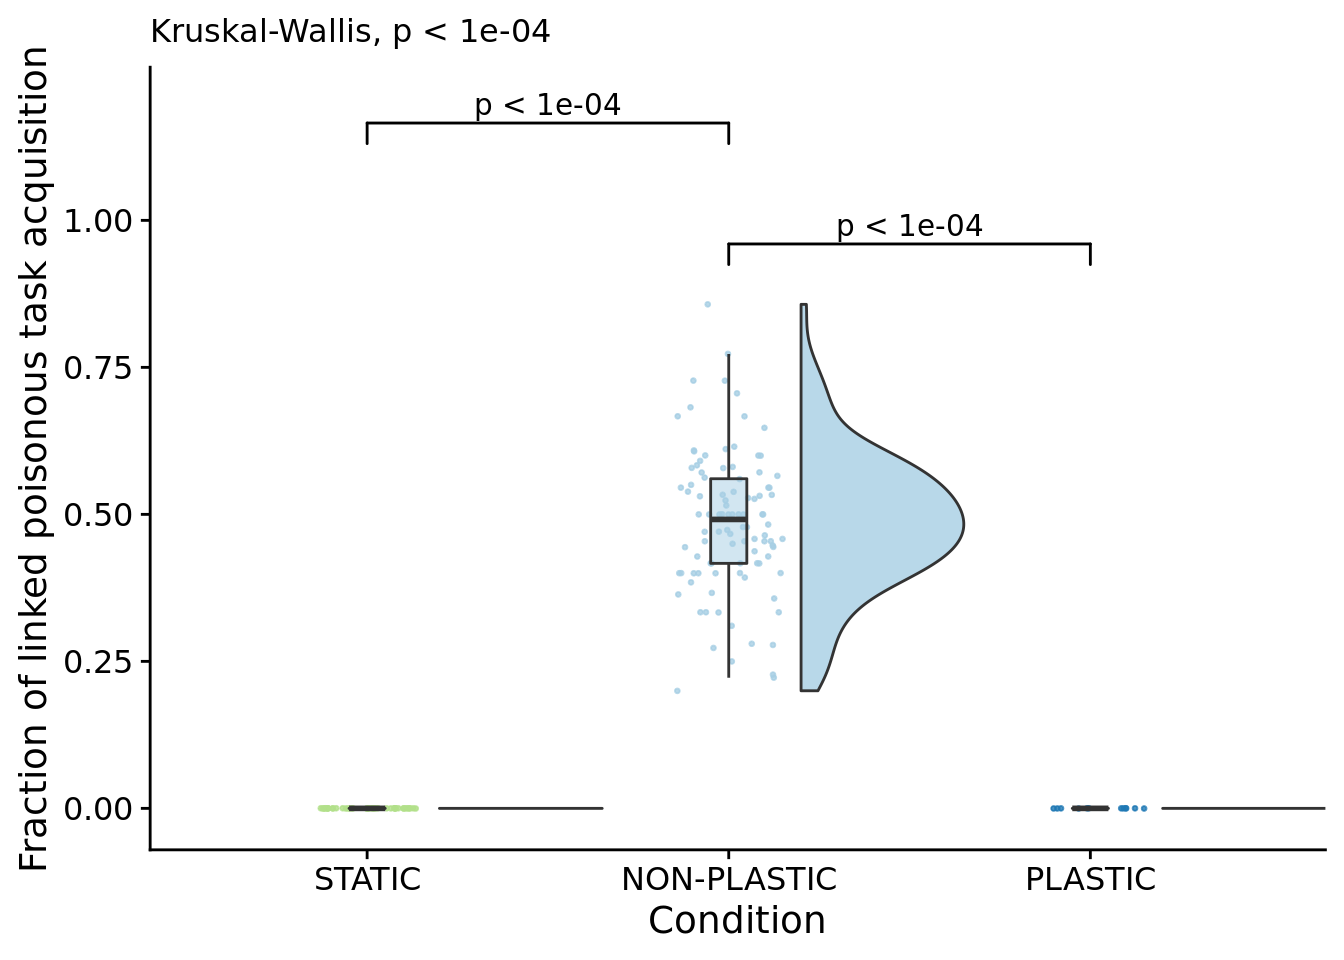
\includegraphics{supplemental-material_files/figure-latex/unnamed-chunk-90-1.pdf}

\hypertarget{what-fraction-of-deleterious-execution-increases-occur-in-unexpressed-phenotype-as-cryptic-variation}{%
\section{What fraction of deleterious execution increases occur in unexpressed phenotype (as cryptic variation)?}\label{what-fraction-of-deleterious-execution-increases-occur-in-unexpressed-phenotype-as-cryptic-variation}}

\begin{Shaded}
\begin{Highlighting}[]
\KeywordTok{ggplot}\NormalTok{(}\KeywordTok{filter}\NormalTok{(summary_data, dominant_lineage_num_times_hitchhike_inst_exec_increases}\OperatorTok{>}\DecValTok{0} \OperatorTok{&}\StringTok{ }\NormalTok{condition}\OperatorTok{==}\StringTok{"PLASTIC"}\NormalTok{), }\KeywordTok{aes}\NormalTok{(}\DataTypeTok{x=}\NormalTok{frac_unexpressed_hitchhiker_inc)) }\OperatorTok{+}
\StringTok{  }\KeywordTok{geom_density}\NormalTok{() }\OperatorTok{+}
\StringTok{  }\KeywordTok{facet_grid}\NormalTok{(}
\NormalTok{    condition}\OperatorTok{~}\NormalTok{POISON_PENALTY,}
    \DataTypeTok{labeller=}\NormalTok{label_both,}
    \DataTypeTok{scales=}\StringTok{"free_y"}
\NormalTok{  ) }\OperatorTok{+}
\StringTok{  }\KeywordTok{theme}\NormalTok{(}
    \DataTypeTok{legend.position=}\StringTok{"none"}
\NormalTok{  )}
\end{Highlighting}
\end{Shaded}

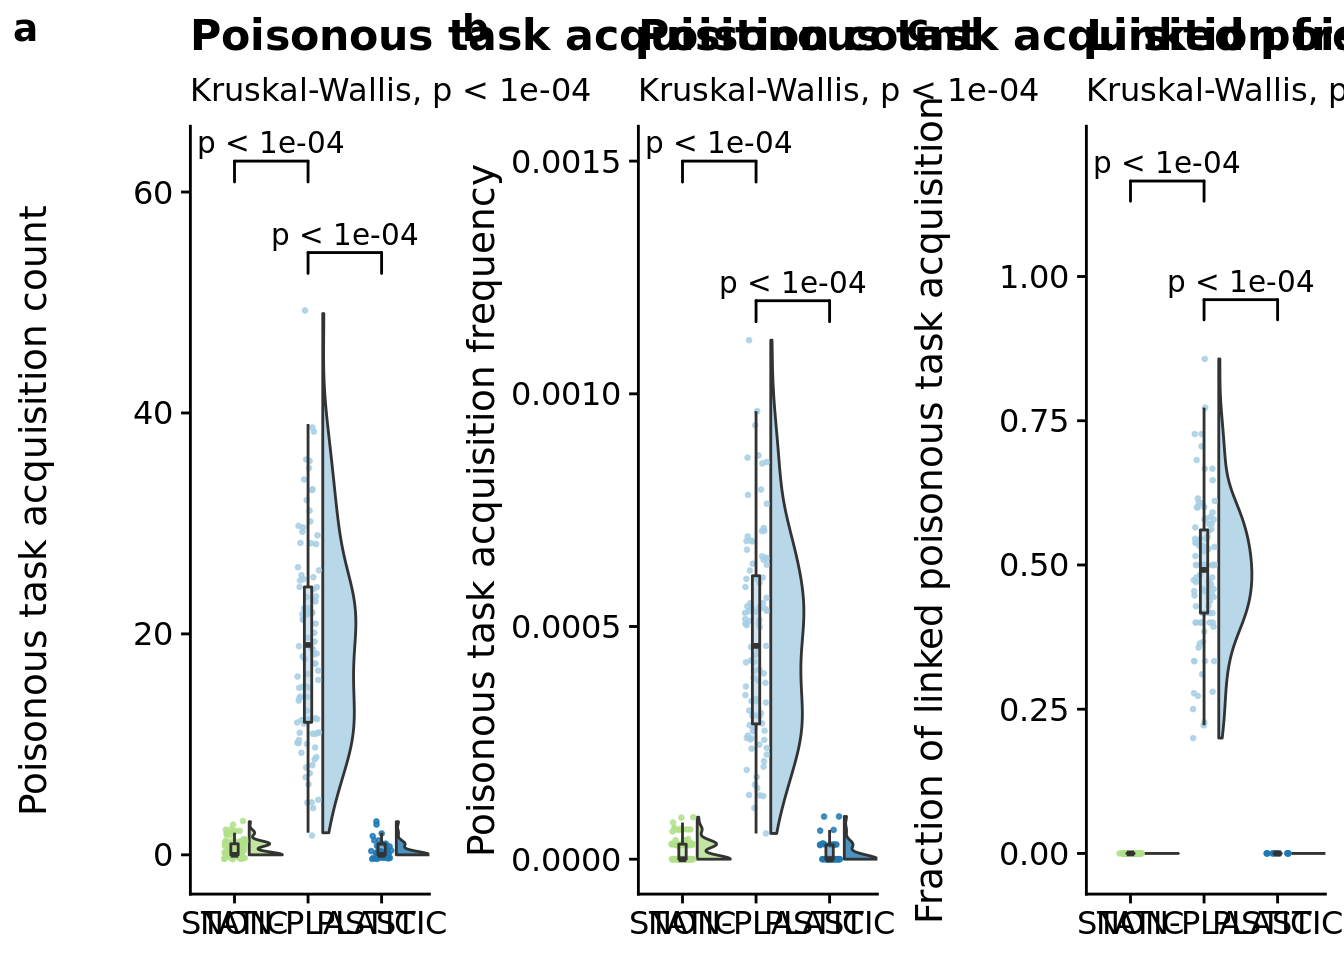
\includegraphics{supplemental-material_files/figure-latex/unnamed-chunk-91-1.pdf}

\begin{Shaded}
\begin{Highlighting}[]
\NormalTok{denom <-}\StringTok{ }\KeywordTok{sum}\NormalTok{(}\KeywordTok{filter}\NormalTok{(summary_data, condition}\OperatorTok{==}\StringTok{"PLASTIC"} \OperatorTok{&}\StringTok{ }\NormalTok{POISON_PENALTY}\OperatorTok{==}\FloatTok{0.1}\NormalTok{)}\OperatorTok{$}\NormalTok{dominant_lineage_num_times_hitchhike_inst_exec_increases)}
\NormalTok{num <-}\StringTok{ }\KeywordTok{sum}\NormalTok{(}\KeywordTok{filter}\NormalTok{(summary_data, condition}\OperatorTok{==}\StringTok{"PLASTIC"} \OperatorTok{&}\StringTok{ }\NormalTok{POISON_PENALTY}\OperatorTok{==}\FloatTok{0.1}\NormalTok{)}\OperatorTok{$}\NormalTok{dominant_lineage_num_times_hitchhike_inst_exec_increases_in_unexpressed_phenotype)}
\KeywordTok{paste0}\NormalTok{(}\StringTok{"PLASTIC: "}\NormalTok{, num}\OperatorTok{/}\NormalTok{denom, }\StringTok{" ("}\NormalTok{, num, }\StringTok{"/"}\NormalTok{, denom, }\StringTok{")"}\NormalTok{)}
\end{Highlighting}
\end{Shaded}

\begin{verbatim}
## [1] "PLASTIC: 0.0555555555555556 (1/18)"
\end{verbatim}

\hypertarget{manuscript-figures-2}{%
\section{Manuscript figures}\label{manuscript-figures-2}}

\begin{Shaded}
\begin{Highlighting}[]
\NormalTok{grid <-}\StringTok{ }\KeywordTok{plot_grid}\NormalTok{(}
\NormalTok{  poison_increases_fig }\OperatorTok{+}
\StringTok{    }\KeywordTok{theme}\NormalTok{(}
      \DataTypeTok{axis.title.x=}\KeywordTok{element_blank}\NormalTok{()}
\NormalTok{    ) }\OperatorTok{+}
\StringTok{    }\KeywordTok{ggtitle}\NormalTok{(}\StringTok{"Deleterious function acquisition count"}\NormalTok{),}
\NormalTok{  poison_increases_per_gen_fig }\OperatorTok{+}
\StringTok{    }\KeywordTok{theme}\NormalTok{(}
      \DataTypeTok{axis.title.x=}\KeywordTok{element_blank}\NormalTok{()}
\NormalTok{    ) }\OperatorTok{+}
\StringTok{    }\KeywordTok{ggtitle}\NormalTok{(}\StringTok{"Deleterious function acquisition frequency"}\NormalTok{),}
\NormalTok{  linked_trait_change_fig }\OperatorTok{+}
\StringTok{    }\KeywordTok{theme}\NormalTok{(}
      \DataTypeTok{axis.title.x=}\KeywordTok{element_blank}\NormalTok{()}
\NormalTok{    ) }\OperatorTok{+}
\StringTok{    }\KeywordTok{ggtitle}\NormalTok{(}\StringTok{"Linked deleterious function acquisition"}\NormalTok{),}
  \DataTypeTok{nrow=}\DecValTok{1}\NormalTok{,}
  \DataTypeTok{align=}\StringTok{"v"}\NormalTok{,}
  \DataTypeTok{labels=}\StringTok{"auto"}
\NormalTok{)}
\KeywordTok{save_plot}\NormalTok{(}
   \KeywordTok{paste0}\NormalTok{(working_directory, }\StringTok{"plots/"}\NormalTok{, }\StringTok{"poison-accumulation-panel.pdf"}\NormalTok{),}
\NormalTok{   grid,}
   \DataTypeTok{base_height=}\DecValTok{6}\NormalTok{,}
   \DataTypeTok{base_asp=}\DecValTok{3}\OperatorTok{/}\DecValTok{1}
\NormalTok{)}
\NormalTok{grid}
\end{Highlighting}
\end{Shaded}

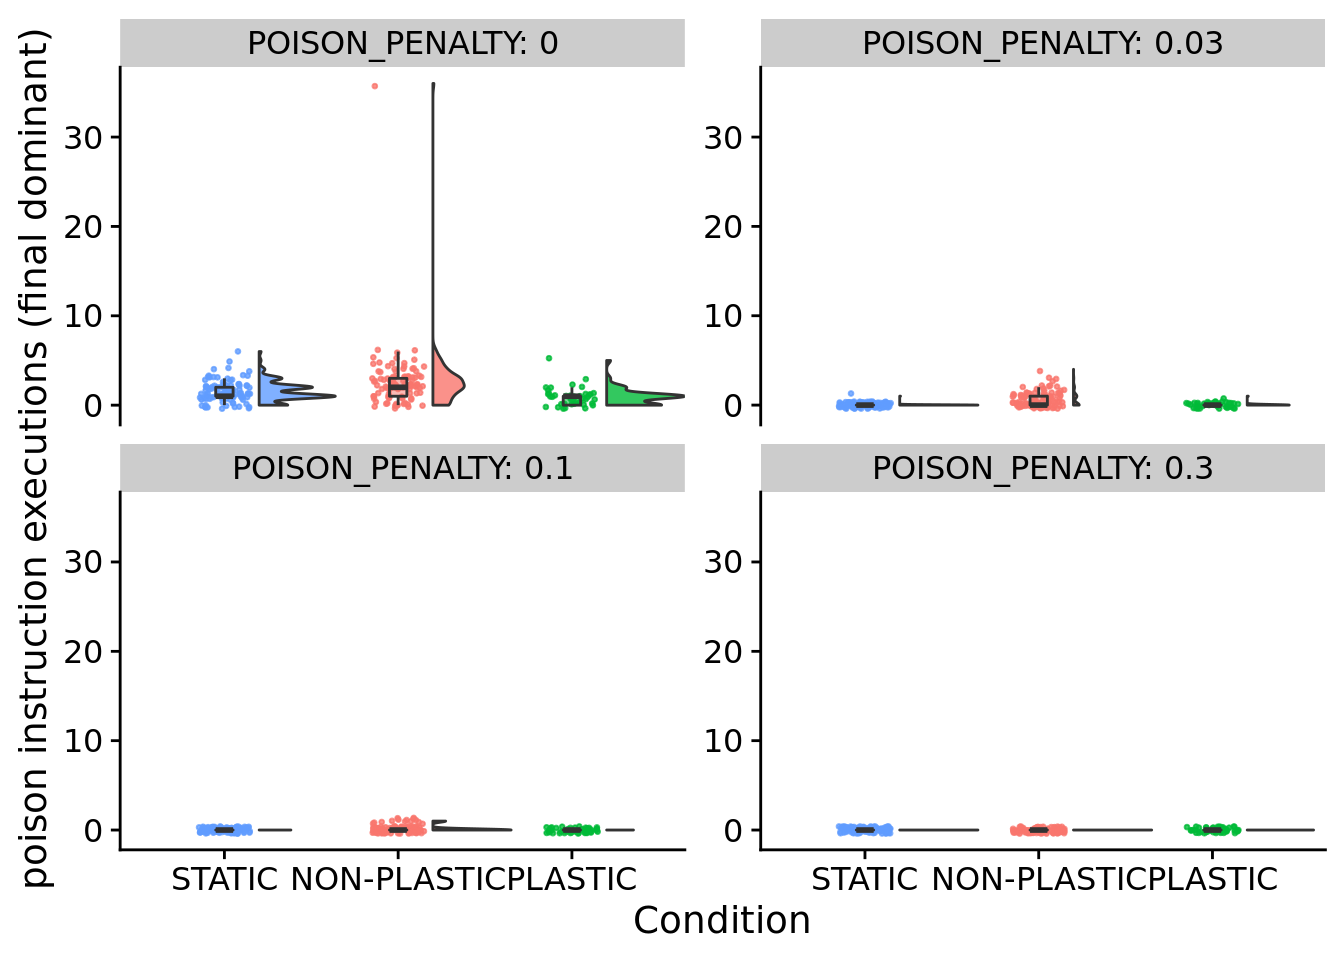
\includegraphics{supplemental-material_files/figure-latex/unnamed-chunk-93-1.pdf}

\hypertarget{regulation-in-avida}{%
\chapter{Regulation in Avida}\label{regulation-in-avida}}

\hypertarget{overview-4}{%
\section{Overview}\label{overview-4}}

\begin{Shaded}
\begin{Highlighting}[]
\NormalTok{total_updates <-}\StringTok{ }\DecValTok{200000}
\NormalTok{replicates <-}\StringTok{ }\DecValTok{100}

\NormalTok{all_traits <-}\StringTok{ }\KeywordTok{c}\NormalTok{(}\StringTok{"not"}\NormalTok{,}\StringTok{"nand"}\NormalTok{,}\StringTok{"and"}\NormalTok{,}\StringTok{"ornot"}\NormalTok{,}\StringTok{"or"}\NormalTok{,}\StringTok{"andnot"}\NormalTok{)}
\NormalTok{traits_set_a <-}\StringTok{ }\KeywordTok{c}\NormalTok{(}\StringTok{"not"}\NormalTok{, }\StringTok{"and"}\NormalTok{, }\StringTok{"or"}\NormalTok{)}
\NormalTok{traits_set_b <-}\StringTok{ }\KeywordTok{c}\NormalTok{(}\StringTok{"nand"}\NormalTok{, }\StringTok{"ornot"}\NormalTok{, }\StringTok{"andnot"}\NormalTok{)}

\CommentTok{# Relative location of data.}
\NormalTok{working_directory <-}\StringTok{ "experiments/2021-02-08-evo-dynamics/analysis/"} \CommentTok{# << For bookdown}
\CommentTok{# working_directory <- "./"                                              # << For local analysis}
\end{Highlighting}
\end{Shaded}

\hypertarget{analysis-dependencies-4}{%
\section{Analysis dependencies}\label{analysis-dependencies-4}}

Load all required R libraries.

\begin{Shaded}
\begin{Highlighting}[]
\KeywordTok{library}\NormalTok{(ggplot2)}
\KeywordTok{library}\NormalTok{(tidyverse)}
\KeywordTok{library}\NormalTok{(cowplot)}
\KeywordTok{library}\NormalTok{(RColorBrewer)}
\KeywordTok{library}\NormalTok{(Hmisc)}
\KeywordTok{library}\NormalTok{(boot)}
\KeywordTok{source}\NormalTok{(}\StringTok{"https://gist.githubusercontent.com/benmarwick/2a1bb0133ff568cbe28d/raw/fb53bd97121f7f9ce947837ef1a4c65a73bffb3f/geom_flat_violin.R"}\NormalTok{)}
\end{Highlighting}
\end{Shaded}

These analyses were conducted/knitted with the following computing environment:

\begin{Shaded}
\begin{Highlighting}[]
\KeywordTok{print}\NormalTok{(version)}
\end{Highlighting}
\end{Shaded}

\begin{verbatim}
##                _                           
## platform       x86_64-pc-linux-gnu         
## arch           x86_64                      
## os             linux-gnu                   
## system         x86_64, linux-gnu           
## status                                     
## major          4                           
## minor          1.3                         
## year           2022                        
## month          03                          
## day            10                          
## svn rev        81868                       
## language       R                           
## version.string R version 4.1.3 (2022-03-10)
## nickname       One Push-Up
\end{verbatim}

\hypertarget{setup-4}{%
\section{Setup}\label{setup-4}}

\begin{Shaded}
\begin{Highlighting}[]
\NormalTok{trace_summary_data_loc <-}\StringTok{ }\KeywordTok{paste0}\NormalTok{(working_directory, }\StringTok{"data/trace_summary.csv"}\NormalTok{)}
\NormalTok{trace_summary_data <-}\StringTok{ }\KeywordTok{read.csv}\NormalTok{(trace_summary_data_loc, }\DataTypeTok{na.strings=}\StringTok{"NONE"}\NormalTok{)}

\NormalTok{trace_summary_data}\OperatorTok{$}\NormalTok{DISABLE_REACTION_SENSORS <-}\StringTok{ }\KeywordTok{as.factor}\NormalTok{(trace_summary_data}\OperatorTok{$}\NormalTok{DISABLE_REACTION_SENSORS)}
\NormalTok{trace_summary_data}\OperatorTok{$}\NormalTok{chg_env <-}\StringTok{ }\NormalTok{trace_summary_data}\OperatorTok{$}\NormalTok{chg_env }\OperatorTok{==}\StringTok{ "True"}
\NormalTok{trace_summary_data}\OperatorTok{$}\NormalTok{sensors <-}\StringTok{ }\NormalTok{trace_summary_data}\OperatorTok{$}\NormalTok{DISABLE_REACTION_SENSORS }\OperatorTok{==}\StringTok{ "0"}


\NormalTok{env_label_fun <-}\StringTok{ }\ControlFlowTok{function}\NormalTok{(chg_env) \{}
  \ControlFlowTok{if}\NormalTok{ (chg_env) \{}
    \KeywordTok{return}\NormalTok{(}\StringTok{"Fluctuating"}\NormalTok{)}
\NormalTok{  \} }\ControlFlowTok{else}\NormalTok{ \{}
    \KeywordTok{return}\NormalTok{(}\StringTok{"Constant"}\NormalTok{)}
\NormalTok{  \}}
\NormalTok{\}}

\NormalTok{sensors_label_fun <-}\StringTok{ }\ControlFlowTok{function}\NormalTok{(has_sensors) \{}
  \ControlFlowTok{if}\NormalTok{ (has_sensors) \{}
    \KeywordTok{return}\NormalTok{(}\StringTok{"Sensors"}\NormalTok{)}
\NormalTok{  \} }\ControlFlowTok{else}\NormalTok{ \{}
    \KeywordTok{return}\NormalTok{(}\StringTok{"No sensors"}\NormalTok{)}
\NormalTok{  \}}
\NormalTok{\}}

\CommentTok{# note that this labeler makes assumptions about how we set up our experiment}
\NormalTok{condition_label_fun <-}\StringTok{ }\ControlFlowTok{function}\NormalTok{(has_sensors, env_chg) \{}
  \ControlFlowTok{if}\NormalTok{ (has_sensors }\OperatorTok{&&}\StringTok{ }\NormalTok{env_chg) \{}
    \KeywordTok{return}\NormalTok{(}\StringTok{"PLASTIC"}\NormalTok{)}
\NormalTok{  \} }\ControlFlowTok{else} \ControlFlowTok{if}\NormalTok{ (env_chg) \{}
    \KeywordTok{return}\NormalTok{(}\StringTok{"NON-PLASTIC"}\NormalTok{)}
\NormalTok{  \} }\ControlFlowTok{else}\NormalTok{ \{}
    \KeywordTok{return}\NormalTok{(}\StringTok{"STATIC"}\NormalTok{)}
\NormalTok{  \}}
\NormalTok{\}}

\NormalTok{trace_summary_data}\OperatorTok{$}\NormalTok{env_label <-}\StringTok{ }\KeywordTok{mapply}\NormalTok{(}
\NormalTok{  env_label_fun,}
\NormalTok{  trace_summary_data}\OperatorTok{$}\NormalTok{chg_env}
\NormalTok{)}
\NormalTok{trace_summary_data}\OperatorTok{$}\NormalTok{sensors_label <-}\StringTok{ }\KeywordTok{mapply}\NormalTok{(}
\NormalTok{  sensors_label_fun,}
\NormalTok{  trace_summary_data}\OperatorTok{$}\NormalTok{sensors}
\NormalTok{)}
\NormalTok{trace_summary_data}\OperatorTok{$}\NormalTok{condition <-}\StringTok{ }\KeywordTok{mapply}\NormalTok{(}
\NormalTok{  condition_label_fun,}
\NormalTok{  trace_summary_data}\OperatorTok{$}\NormalTok{sensors,}
\NormalTok{  trace_summary_data}\OperatorTok{$}\NormalTok{chg_env}
\NormalTok{)}

\CommentTok{####### misc #######}
\CommentTok{# Configure our default graphing theme}
\KeywordTok{theme_set}\NormalTok{(}\KeywordTok{theme_cowplot}\NormalTok{())}
\KeywordTok{dir.create}\NormalTok{(}\KeywordTok{paste0}\NormalTok{(working_directory, }\StringTok{"plots"}\NormalTok{), }\DataTypeTok{showWarnings=}\OtherTok{FALSE}\NormalTok{)}
\end{Highlighting}
\end{Shaded}

\hypertarget{how-many-instructions-do-plastic-genomes-toggle-depending-on-environmental-context}{%
\section{How many instructions do plastic genomes toggle depending on environmental context?}\label{how-many-instructions-do-plastic-genomes-toggle-depending-on-environmental-context}}

\begin{Shaded}
\begin{Highlighting}[]
\KeywordTok{ggplot}\NormalTok{(trace_summary_data, }\KeywordTok{aes}\NormalTok{(}\DataTypeTok{x=}\NormalTok{dominant_num_toggled_sites)) }\OperatorTok{+}
\StringTok{    }\KeywordTok{geom_histogram}\NormalTok{(}
      \DataTypeTok{binwidth=}\DecValTok{1}\NormalTok{,}
      \DataTypeTok{color=}\StringTok{"black"}
\NormalTok{    ) }\OperatorTok{+}
\StringTok{    }\KeywordTok{scale_fill_brewer}\NormalTok{(}
      \DataTypeTok{palette=}\StringTok{"Paired"}
\NormalTok{    ) }\OperatorTok{+}
\StringTok{    }\KeywordTok{scale_color_brewer}\NormalTok{(}
      \DataTypeTok{palette=}\StringTok{"Paired"}
\NormalTok{    ) }\OperatorTok{+}
\StringTok{    }\KeywordTok{scale_x_continuous}\NormalTok{(}
      \DataTypeTok{breaks=}\KeywordTok{seq}\NormalTok{(}\DecValTok{0}\NormalTok{, }\KeywordTok{max}\NormalTok{(trace_summary_data}\OperatorTok{$}\NormalTok{dominant_num_toggled_sites)}\OperatorTok{+}\DecValTok{1}\NormalTok{)}
\NormalTok{    ) }\OperatorTok{+}
\StringTok{    }\KeywordTok{theme}\NormalTok{(}
      \DataTypeTok{legend.position=}\StringTok{"none"}
\NormalTok{    )}
\end{Highlighting}
\end{Shaded}

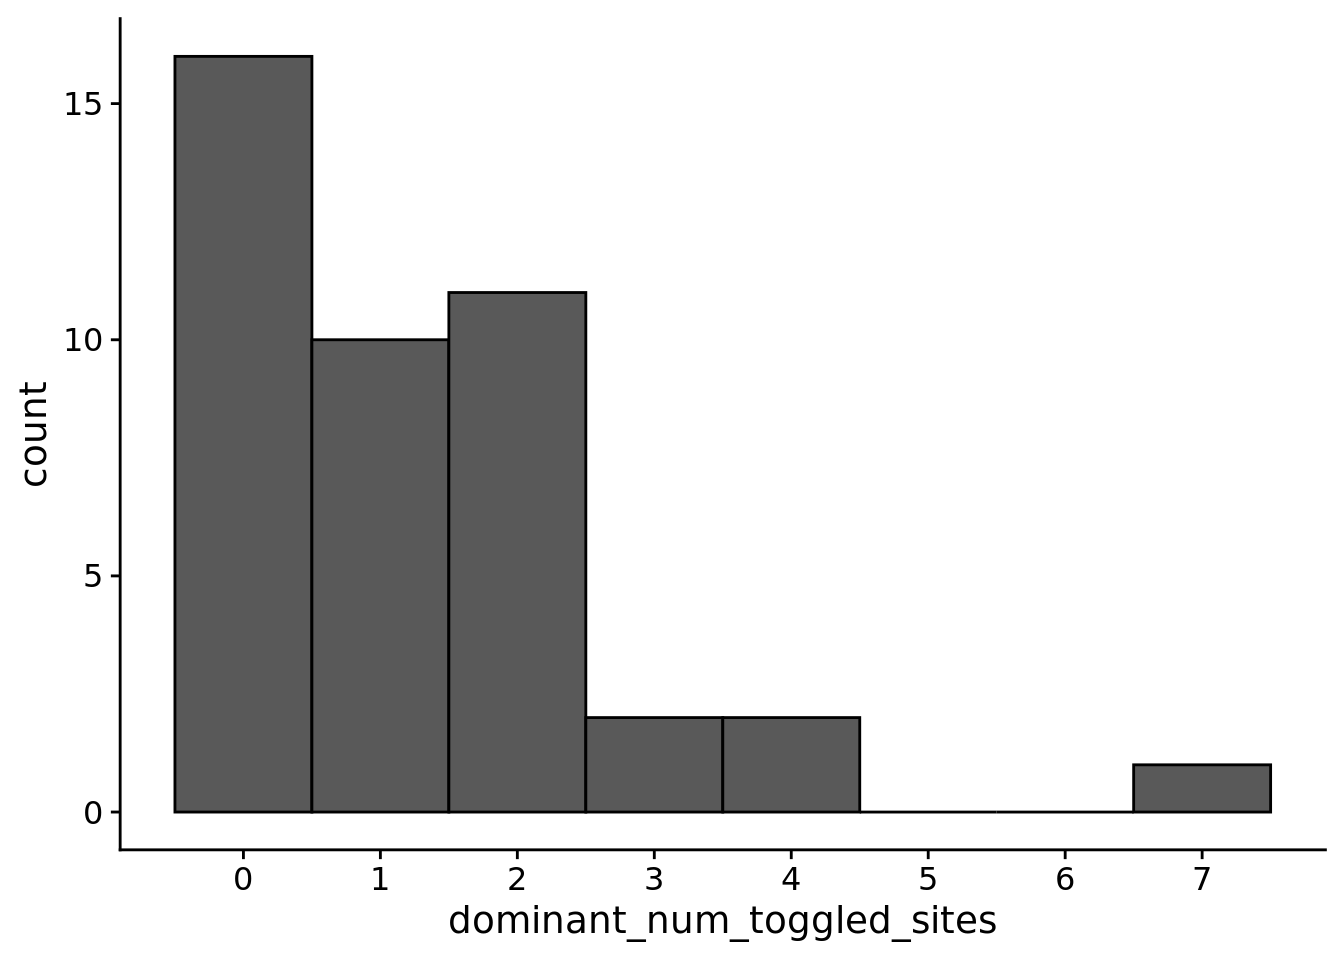
\includegraphics{supplemental-material_files/figure-latex/unnamed-chunk-98-1.pdf}

\begin{Shaded}
\begin{Highlighting}[]
\KeywordTok{ggsave}\NormalTok{(}\KeywordTok{paste0}\NormalTok{(working_directory, }\StringTok{"plots/"}\NormalTok{, }\StringTok{"toggled-sites.png"}\NormalTok{))}
\end{Highlighting}
\end{Shaded}

\begin{verbatim}
## Saving 6.5 x 4.5 in image
\end{verbatim}

\hypertarget{what-is-the-distrubution-of-toggled-sequence-sizes}{%
\section{What is the distrubution of toggled sequence sizes?}\label{what-is-the-distrubution-of-toggled-sequence-sizes}}

\begin{Shaded}
\begin{Highlighting}[]
\NormalTok{chunk_sizes <-}\StringTok{ }\KeywordTok{data.frame}\NormalTok{(}
  \DataTypeTok{size=}\KeywordTok{integer}\NormalTok{()}
\NormalTok{)}
\ControlFlowTok{for}\NormalTok{ (sizes }\ControlFlowTok{in}\NormalTok{ trace_summary_data}\OperatorTok{$}\NormalTok{dominant_toggled_chunk_sizes) \{}
  \ControlFlowTok{if}\NormalTok{ (sizes }\OperatorTok{==}\StringTok{ ""}\NormalTok{) \{ }\ControlFlowTok{next}\NormalTok{ \}}
\NormalTok{  sizes <-}\StringTok{ }\KeywordTok{unlist}\NormalTok{(}\KeywordTok{lapply}\NormalTok{(}\KeywordTok{str_split}\NormalTok{(sizes, }\StringTok{';'}\NormalTok{), as.integer))}
\NormalTok{  chunk_sizes <-}\StringTok{ }\KeywordTok{rbind}\NormalTok{(chunk_sizes, }\KeywordTok{data.frame}\NormalTok{(}\DataTypeTok{size=}\KeywordTok{c}\NormalTok{(sizes)))}
\NormalTok{\}}

\KeywordTok{ggplot}\NormalTok{(chunk_sizes, }\KeywordTok{aes}\NormalTok{(}\DataTypeTok{x=}\NormalTok{size)) }\OperatorTok{+}
\StringTok{    }\KeywordTok{geom_histogram}\NormalTok{(}
      \DataTypeTok{binwidth=}\DecValTok{1}\NormalTok{,}
      \DataTypeTok{color=}\StringTok{"black"}
\NormalTok{    ) }\OperatorTok{+}
\StringTok{    }\KeywordTok{scale_fill_brewer}\NormalTok{(}
      \DataTypeTok{palette=}\StringTok{"Paired"}
\NormalTok{    ) }\OperatorTok{+}
\StringTok{    }\KeywordTok{scale_color_brewer}\NormalTok{(}
      \DataTypeTok{palette=}\StringTok{"Paired"}
\NormalTok{    ) }\OperatorTok{+}
\StringTok{    }\KeywordTok{scale_x_continuous}\NormalTok{(}
      \DataTypeTok{name=}\StringTok{"toggled sequence size"}\NormalTok{,}
      \DataTypeTok{breaks=}\KeywordTok{seq}\NormalTok{(}\DecValTok{0}\NormalTok{, }\DecValTok{10}\NormalTok{),}
      \DataTypeTok{limits=}\KeywordTok{c}\NormalTok{(}\DecValTok{0}\NormalTok{, }\DecValTok{10}\NormalTok{)}
\NormalTok{    ) }\OperatorTok{+}
\StringTok{    }\KeywordTok{theme}\NormalTok{(}
      \DataTypeTok{legend.position=}\StringTok{"none"}
\NormalTok{    )}
\end{Highlighting}
\end{Shaded}

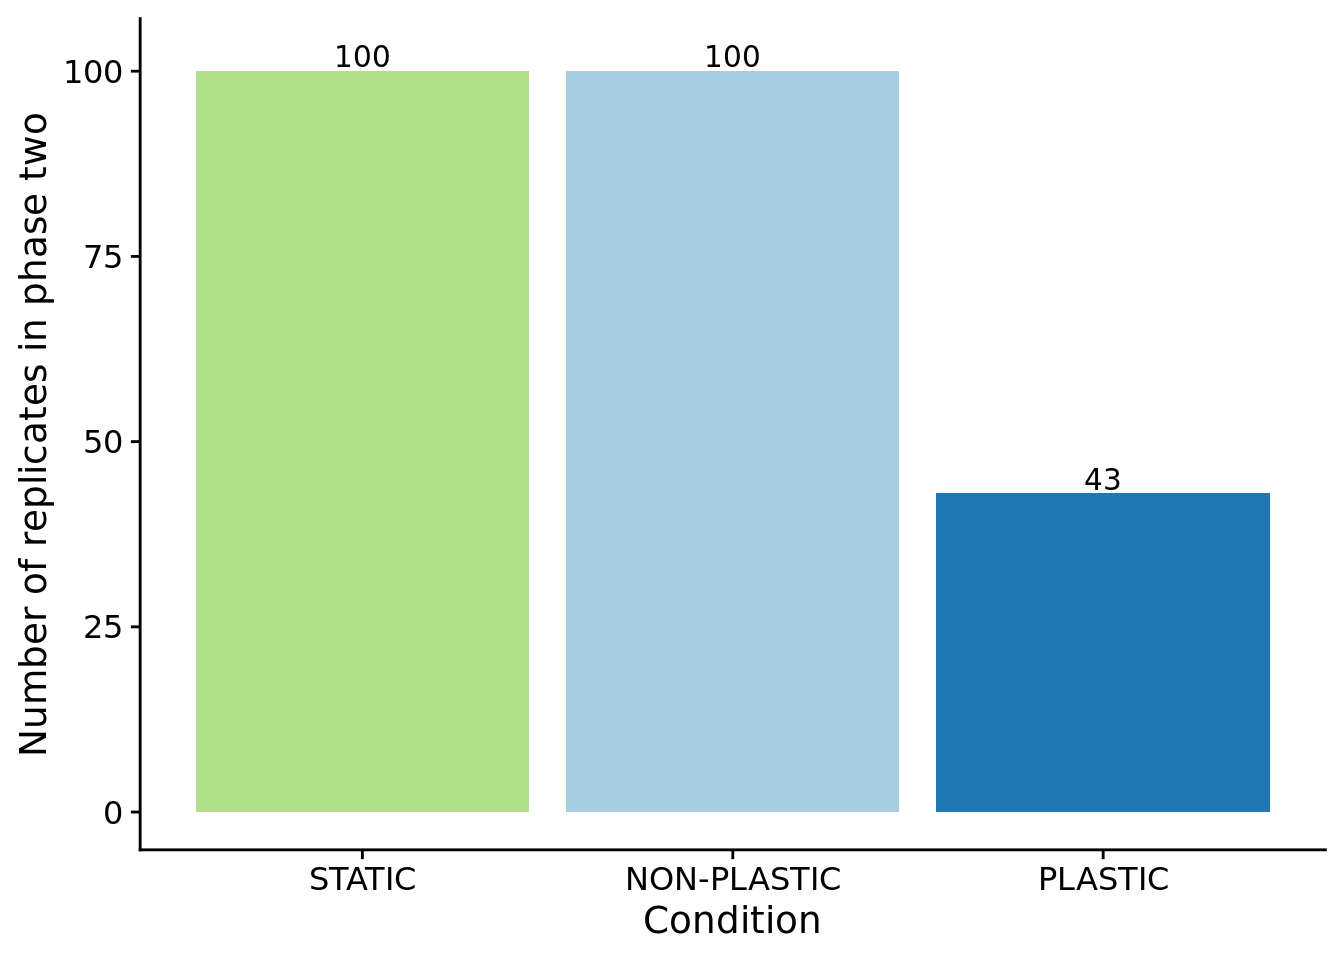
\includegraphics{supplemental-material_files/figure-latex/unnamed-chunk-99-1.pdf}

\begin{Shaded}
\begin{Highlighting}[]
\KeywordTok{ggsave}\NormalTok{(}\KeywordTok{paste0}\NormalTok{(working_directory, }\StringTok{"plots/"}\NormalTok{, }\StringTok{"toggled-chunk-sizes.png"}\NormalTok{))}
\end{Highlighting}
\end{Shaded}

\begin{verbatim}
## Saving 6.5 x 4.5 in image
\end{verbatim}

\hypertarget{evolutionary-change-variable-length-genomes}{%
\chapter{Evolutionary change (variable length genomes)}\label{evolutionary-change-variable-length-genomes}}

\hypertarget{overview-5}{%
\section{Overview}\label{overview-5}}

\begin{Shaded}
\begin{Highlighting}[]
\NormalTok{total_updates <-}\StringTok{ }\DecValTok{200000}
\NormalTok{replicates <-}\StringTok{ }\DecValTok{100}

\NormalTok{all_traits <-}\StringTok{ }\KeywordTok{c}\NormalTok{(}\StringTok{"not"}\NormalTok{,}\StringTok{"nand"}\NormalTok{,}\StringTok{"and"}\NormalTok{,}\StringTok{"ornot"}\NormalTok{,}\StringTok{"or"}\NormalTok{,}\StringTok{"andnot"}\NormalTok{)}
\NormalTok{traits_set_a <-}\StringTok{ }\KeywordTok{c}\NormalTok{(}\StringTok{"not"}\NormalTok{, }\StringTok{"and"}\NormalTok{, }\StringTok{"or"}\NormalTok{)}
\NormalTok{traits_set_b <-}\StringTok{ }\KeywordTok{c}\NormalTok{(}\StringTok{"nand"}\NormalTok{, }\StringTok{"ornot"}\NormalTok{, }\StringTok{"andnot"}\NormalTok{)}

\CommentTok{# Relative location of data.}
\NormalTok{working_directory <-}\StringTok{ "experiments/2021-01-30-evo-dynamics/analysis/"} \CommentTok{# << For bookdown}
\CommentTok{# working_directory <- "./"                                              # << For local analysis}
\end{Highlighting}
\end{Shaded}

\hypertarget{analysis-dependencies-5}{%
\section{Analysis dependencies}\label{analysis-dependencies-5}}

Load all required R libraries.

\begin{Shaded}
\begin{Highlighting}[]
\KeywordTok{library}\NormalTok{(ggplot2)}
\KeywordTok{library}\NormalTok{(tidyverse)}
\KeywordTok{library}\NormalTok{(cowplot)}
\KeywordTok{library}\NormalTok{(RColorBrewer)}
\KeywordTok{library}\NormalTok{(Hmisc)}
\KeywordTok{library}\NormalTok{(boot)}
\KeywordTok{source}\NormalTok{(}\StringTok{"https://gist.githubusercontent.com/benmarwick/2a1bb0133ff568cbe28d/raw/fb53bd97121f7f9ce947837ef1a4c65a73bffb3f/geom_flat_violin.R"}\NormalTok{)}
\end{Highlighting}
\end{Shaded}

These analyses were conducted/knitted with the following computing environment:

\begin{Shaded}
\begin{Highlighting}[]
\KeywordTok{print}\NormalTok{(version)}
\end{Highlighting}
\end{Shaded}

\begin{verbatim}
##                _                           
## platform       x86_64-pc-linux-gnu         
## arch           x86_64                      
## os             linux-gnu                   
## system         x86_64, linux-gnu           
## status                                     
## major          4                           
## minor          1.3                         
## year           2022                        
## month          03                          
## day            10                          
## svn rev        81868                       
## language       R                           
## version.string R version 4.1.3 (2022-03-10)
## nickname       One Push-Up
\end{verbatim}

\hypertarget{setup-5}{%
\section{Setup}\label{setup-5}}

\begin{Shaded}
\begin{Highlighting}[]
\NormalTok{summary_data_loc <-}\StringTok{ }\KeywordTok{paste0}\NormalTok{(working_directory, }\StringTok{"data/aggregate.csv"}\NormalTok{)}
\NormalTok{summary_data <-}\StringTok{ }\KeywordTok{read.csv}\NormalTok{(summary_data_loc, }\DataTypeTok{na.strings=}\StringTok{"NONE"}\NormalTok{)}

\NormalTok{summary_data}\OperatorTok{$}\NormalTok{DISABLE_REACTION_SENSORS <-}\StringTok{ }\KeywordTok{as.factor}\NormalTok{(summary_data}\OperatorTok{$}\NormalTok{DISABLE_REACTION_SENSORS)}
\NormalTok{summary_data}\OperatorTok{$}\NormalTok{chg_env <-}\StringTok{ }\NormalTok{summary_data}\OperatorTok{$}\NormalTok{chg_env }\OperatorTok{==}\StringTok{ "True"}
\NormalTok{summary_data}\OperatorTok{$}\NormalTok{dominant_plastic_odd_even <-}\StringTok{ }\KeywordTok{as.factor}\NormalTok{(summary_data}\OperatorTok{$}\NormalTok{dominant_plastic_odd_even)}
\NormalTok{summary_data}\OperatorTok{$}\NormalTok{sensors <-}\StringTok{ }\NormalTok{summary_data}\OperatorTok{$}\NormalTok{DISABLE_REACTION_SENSORS }\OperatorTok{==}\StringTok{ "0"}
\NormalTok{summary_data}\OperatorTok{$}\NormalTok{is_plastic <-}\StringTok{ }\NormalTok{summary_data}\OperatorTok{$}\NormalTok{dominant_plastic_odd_even }\OperatorTok{==}\StringTok{ "True"}

\NormalTok{env_label_fun <-}\StringTok{ }\ControlFlowTok{function}\NormalTok{(chg_env) \{}
  \ControlFlowTok{if}\NormalTok{ (chg_env) \{}
    \KeywordTok{return}\NormalTok{(}\StringTok{"Fluctuating"}\NormalTok{)}
\NormalTok{  \} }\ControlFlowTok{else}\NormalTok{ \{}
    \KeywordTok{return}\NormalTok{(}\StringTok{"Constant"}\NormalTok{)}
\NormalTok{  \}}
\NormalTok{\}}

\NormalTok{sensors_label_fun <-}\StringTok{ }\ControlFlowTok{function}\NormalTok{(has_sensors) \{}
  \ControlFlowTok{if}\NormalTok{ (has_sensors) \{}
    \KeywordTok{return}\NormalTok{(}\StringTok{"Sensors"}\NormalTok{)}
\NormalTok{  \} }\ControlFlowTok{else}\NormalTok{ \{}
    \KeywordTok{return}\NormalTok{(}\StringTok{"No sensors"}\NormalTok{)}
\NormalTok{  \}}
\NormalTok{\}}

\CommentTok{# note that this labeler makes assumptions about how we set up our experiment}
\NormalTok{condition_label_fun <-}\StringTok{ }\ControlFlowTok{function}\NormalTok{(has_sensors, env_chg) \{}
  \ControlFlowTok{if}\NormalTok{ (has_sensors }\OperatorTok{&&}\StringTok{ }\NormalTok{env_chg) \{}
    \KeywordTok{return}\NormalTok{(}\StringTok{"PLASTIC"}\NormalTok{)}
\NormalTok{  \} }\ControlFlowTok{else} \ControlFlowTok{if}\NormalTok{ (env_chg) \{}
    \KeywordTok{return}\NormalTok{(}\StringTok{"NON-PLASTIC"}\NormalTok{)}
\NormalTok{  \} }\ControlFlowTok{else}\NormalTok{ \{}
    \KeywordTok{return}\NormalTok{(}\StringTok{"STATIC"}\NormalTok{)}
\NormalTok{  \}}
\NormalTok{\}}

\NormalTok{summary_data}\OperatorTok{$}\NormalTok{env_label <-}\StringTok{ }\KeywordTok{mapply}\NormalTok{(}
\NormalTok{  env_label_fun,}
\NormalTok{  summary_data}\OperatorTok{$}\NormalTok{chg_env}
\NormalTok{)}
\NormalTok{summary_data}\OperatorTok{$}\NormalTok{sensors_label <-}\StringTok{ }\KeywordTok{mapply}\NormalTok{(}
\NormalTok{  sensors_label_fun,}
\NormalTok{  summary_data}\OperatorTok{$}\NormalTok{sensors}
\NormalTok{)}
\NormalTok{summary_data}\OperatorTok{$}\NormalTok{condition <-}\StringTok{ }\KeywordTok{mapply}\NormalTok{(}
\NormalTok{  condition_label_fun,}
\NormalTok{  summary_data}\OperatorTok{$}\NormalTok{sensors,}
\NormalTok{  summary_data}\OperatorTok{$}\NormalTok{chg_env}
\NormalTok{)}

\NormalTok{condition_order =}\StringTok{ }\KeywordTok{c}\NormalTok{(}
  \StringTok{"STATIC"}\NormalTok{,}
  \StringTok{"NON-PLASTIC"}\NormalTok{,}
  \StringTok{"PLASTIC"}
\NormalTok{)}

\CommentTok{####### misc #######}
\CommentTok{# Configure our default graphing theme}
\KeywordTok{theme_set}\NormalTok{(}\KeywordTok{theme_cowplot}\NormalTok{())}
\KeywordTok{dir.create}\NormalTok{(}\KeywordTok{paste0}\NormalTok{(working_directory, }\StringTok{"plots"}\NormalTok{), }\DataTypeTok{showWarnings=}\OtherTok{FALSE}\NormalTok{)}
\end{Highlighting}
\end{Shaded}

\hypertarget{evolution-of-phenotypic-plasticity-2}{%
\section{Evolution of phenotypic plasticity}\label{evolution-of-phenotypic-plasticity-2}}

For sensor-enabled populations in fluctuating environments, we only transfered populations containing an optimally plastic genotype to phase two.

\begin{Shaded}
\begin{Highlighting}[]
\NormalTok{summary_data_grouped =}\StringTok{ }\NormalTok{dplyr}\OperatorTok{::}\KeywordTok{group_by}\NormalTok{(summary_data, sensors, env_label, condition)}
\NormalTok{summary_data_group_counts =}\StringTok{ }\NormalTok{dplyr}\OperatorTok{::}\KeywordTok{summarize}\NormalTok{(summary_data_grouped, }\DataTypeTok{n=}\NormalTok{dplyr}\OperatorTok{::}\KeywordTok{n}\NormalTok{())}
\end{Highlighting}
\end{Shaded}

\begin{verbatim}
## `summarise()` has grouped output by 'sensors', 'env_label'. You can override
## using the `.groups` argument.
\end{verbatim}

\begin{Shaded}
\begin{Highlighting}[]
\KeywordTok{ggplot}\NormalTok{(summary_data_group_counts, }\KeywordTok{aes}\NormalTok{(}\DataTypeTok{x=}\NormalTok{condition, }\DataTypeTok{y=}\NormalTok{n, }\DataTypeTok{fill=}\NormalTok{condition)) }\OperatorTok{+}
\StringTok{  }\KeywordTok{geom_col}\NormalTok{(}\DataTypeTok{position=}\KeywordTok{position_dodge}\NormalTok{(}\FloatTok{0.9}\NormalTok{)) }\OperatorTok{+}
\StringTok{  }\KeywordTok{geom_text}\NormalTok{(}\KeywordTok{aes}\NormalTok{(}\DataTypeTok{label=}\NormalTok{n, }\DataTypeTok{y=}\NormalTok{n}\OperatorTok{+}\DecValTok{2}\NormalTok{)) }\OperatorTok{+}
\StringTok{  }\KeywordTok{scale_x_discrete}\NormalTok{(}
    \DataTypeTok{name=}\StringTok{"Condition"}\NormalTok{,}
    \DataTypeTok{limits=}\NormalTok{condition_order}
\NormalTok{  ) }\OperatorTok{+}
\StringTok{  }\KeywordTok{scale_fill_brewer}\NormalTok{(}
    \DataTypeTok{palette=}\StringTok{"Paired"}
\NormalTok{  ) }\OperatorTok{+}
\StringTok{  }\KeywordTok{scale_color_brewer}\NormalTok{(}
    \DataTypeTok{palette=}\StringTok{"Paired"}
\NormalTok{  ) }\OperatorTok{+}
\StringTok{  }\KeywordTok{ylab}\NormalTok{(}\StringTok{"Number of replicates in phase two"}\NormalTok{) }\OperatorTok{+}
\StringTok{  }\KeywordTok{theme}\NormalTok{(}
    \DataTypeTok{legend.position=}\StringTok{"none"}
\NormalTok{  )}
\end{Highlighting}
\end{Shaded}

\includegraphics{supplemental-material_files/figure-latex/unnamed-chunk-104-1.pdf}

We can confirm our expectation that the dominant genotypes in non-plastic conditions are not phenotypically plastic.

\begin{Shaded}
\begin{Highlighting}[]
\NormalTok{summary_data_grouped =}\StringTok{ }\NormalTok{dplyr}\OperatorTok{::}\KeywordTok{group_by}\NormalTok{(summary_data, condition, is_plastic)}
\NormalTok{summary_data_group_counts =}\StringTok{ }\NormalTok{dplyr}\OperatorTok{::}\KeywordTok{summarize}\NormalTok{(summary_data_grouped, }\DataTypeTok{n=}\NormalTok{dplyr}\OperatorTok{::}\KeywordTok{n}\NormalTok{())}
\KeywordTok{ggplot}\NormalTok{(}\KeywordTok{filter}\NormalTok{(summary_data_group_counts, is_plastic), }\KeywordTok{aes}\NormalTok{(}\DataTypeTok{x=}\NormalTok{condition, }\DataTypeTok{y=}\NormalTok{n, }\DataTypeTok{fill=}\NormalTok{condition)) }\OperatorTok{+}
\StringTok{  }\KeywordTok{geom_col}\NormalTok{(}\DataTypeTok{position=}\KeywordTok{position_dodge}\NormalTok{(}\FloatTok{0.9}\NormalTok{)) }\OperatorTok{+}
\StringTok{  }\KeywordTok{scale_x_discrete}\NormalTok{(}
    \DataTypeTok{name=}\StringTok{"Condition"}\NormalTok{,}
    \DataTypeTok{limits=}\NormalTok{condition_order}
\NormalTok{  ) }\OperatorTok{+}
\StringTok{  }\KeywordTok{scale_fill_brewer}\NormalTok{(}
    \DataTypeTok{palette=}\StringTok{"Paired"}
\NormalTok{  ) }\OperatorTok{+}
\StringTok{  }\KeywordTok{scale_color_brewer}\NormalTok{(}
    \DataTypeTok{palette=}\StringTok{"Paired"}
\NormalTok{  ) }\OperatorTok{+}
\StringTok{  }\KeywordTok{geom_text}\NormalTok{(}\KeywordTok{aes}\NormalTok{(}\DataTypeTok{label=}\NormalTok{n, }\DataTypeTok{y=}\NormalTok{n}\OperatorTok{+}\DecValTok{1}\NormalTok{)) }\OperatorTok{+}
\StringTok{  }\KeywordTok{ylab}\NormalTok{(}\StringTok{"Number of replicates with a plastic dominant genotype"}\NormalTok{) }\OperatorTok{+}
\StringTok{  }\KeywordTok{theme}\NormalTok{(}
    \DataTypeTok{legend.position=}\StringTok{"none"}
\NormalTok{  )}
\end{Highlighting}
\end{Shaded}

\includegraphics{supplemental-material_files/figure-latex/unnamed-chunk-105-1.pdf}

\hypertarget{genome-length}{%
\section{Genome length}\label{genome-length}}

Single-instruction insertions and deletions were possible for this experiment, so genome size also evolved.

\begin{Shaded}
\begin{Highlighting}[]
\KeywordTok{ggplot}\NormalTok{(summary_data, }\KeywordTok{aes}\NormalTok{(}\DataTypeTok{x=}\NormalTok{condition, }\DataTypeTok{y=}\NormalTok{dominant_genome_length, }\DataTypeTok{fill=}\NormalTok{condition)) }\OperatorTok{+}
\StringTok{  }\KeywordTok{geom_flat_violin}\NormalTok{(}
    \DataTypeTok{position =} \KeywordTok{position_nudge}\NormalTok{(}\DataTypeTok{x =} \FloatTok{.2}\NormalTok{, }\DataTypeTok{y =} \DecValTok{0}\NormalTok{),}
    \DataTypeTok{alpha =} \FloatTok{.8}
\NormalTok{  ) }\OperatorTok{+}
\StringTok{  }\KeywordTok{geom_point}\NormalTok{(}
    \DataTypeTok{mapping=}\KeywordTok{aes}\NormalTok{(}\DataTypeTok{color=}\NormalTok{condition),}
    \DataTypeTok{position =} \KeywordTok{position_jitter}\NormalTok{(}\DataTypeTok{width =} \FloatTok{.15}\NormalTok{),}
    \DataTypeTok{size =} \FloatTok{.5}\NormalTok{,}
    \DataTypeTok{alpha =} \FloatTok{0.8}
\NormalTok{  ) }\OperatorTok{+}
\StringTok{  }\KeywordTok{geom_boxplot}\NormalTok{(}
    \DataTypeTok{width =} \FloatTok{.1}\NormalTok{,}
    \DataTypeTok{outlier.shape =} \OtherTok{NA}\NormalTok{,}
    \DataTypeTok{alpha =} \FloatTok{0.5}
\NormalTok{  ) }\OperatorTok{+}
\StringTok{  }\KeywordTok{scale_x_discrete}\NormalTok{(}
    \DataTypeTok{name=}\StringTok{"Condition"}\NormalTok{,}
    \DataTypeTok{limits=}\NormalTok{condition_order}
\NormalTok{  ) }\OperatorTok{+}
\StringTok{  }\KeywordTok{scale_fill_brewer}\NormalTok{(}
    \DataTypeTok{palette=}\StringTok{"Paired"}
\NormalTok{  ) }\OperatorTok{+}
\StringTok{  }\KeywordTok{scale_color_brewer}\NormalTok{(}
    \DataTypeTok{palette=}\StringTok{"Paired"}
\NormalTok{  ) }\OperatorTok{+}
\StringTok{  }\KeywordTok{ylab}\NormalTok{(}\StringTok{"Genome length"}\NormalTok{) }\OperatorTok{+}
\StringTok{  }\KeywordTok{theme}\NormalTok{(}
    \DataTypeTok{legend.position=}\StringTok{"none"}
\NormalTok{  )}
\end{Highlighting}
\end{Shaded}

\includegraphics{supplemental-material_files/figure-latex/unnamed-chunk-106-1.pdf}

\begin{Shaded}
\begin{Highlighting}[]
\KeywordTok{kruskal.test}\NormalTok{(}
  \DataTypeTok{formula=}\NormalTok{dominant_genome_length}\OperatorTok{~}\NormalTok{condition,}
  \DataTypeTok{data=}\NormalTok{summary_data}
\NormalTok{)}
\end{Highlighting}
\end{Shaded}

\begin{verbatim}
## 
##  Kruskal-Wallis rank sum test
## 
## data:  dominant_genome_length by condition
## Kruskal-Wallis chi-squared = 82.798, df = 2, p-value < 2.2e-16
\end{verbatim}

\begin{Shaded}
\begin{Highlighting}[]
\KeywordTok{pairwise.wilcox.test}\NormalTok{(}
  \DataTypeTok{x=}\NormalTok{summary_data}\OperatorTok{$}\NormalTok{dominant_genome_length,}
  \DataTypeTok{g=}\NormalTok{summary_data}\OperatorTok{$}\NormalTok{condition,}
  \DataTypeTok{p.adjust.method=}\StringTok{"bonferroni"}\NormalTok{,}
\NormalTok{)}
\end{Highlighting}
\end{Shaded}

\begin{verbatim}
## 
##  Pairwise comparisons using Wilcoxon rank sum test with continuity correction 
## 
## data:  summary_data$dominant_genome_length and summary_data$condition 
## 
##         NON-PLASTIC PLASTIC
## PLASTIC 1.8e-10     -      
## STATIC  < 2e-16     1      
## 
## P value adjustment method: bonferroni
\end{verbatim}

\begin{Shaded}
\begin{Highlighting}[]
\KeywordTok{median}\NormalTok{(}\KeywordTok{filter}\NormalTok{(summary_data, condition}\OperatorTok{==}\StringTok{"PLASTIC"}\NormalTok{)}\OperatorTok{$}\NormalTok{phylo_mrca_changes)}
\end{Highlighting}
\end{Shaded}

\begin{verbatim}
## [1] 45
\end{verbatim}

\begin{Shaded}
\begin{Highlighting}[]
\KeywordTok{median}\NormalTok{(}\KeywordTok{filter}\NormalTok{(summary_data, condition}\OperatorTok{==}\StringTok{"STATIC"}\NormalTok{)}\OperatorTok{$}\NormalTok{phylo_mrca_changes)}
\end{Highlighting}
\end{Shaded}

\begin{verbatim}
## [1] 47
\end{verbatim}

\begin{Shaded}
\begin{Highlighting}[]
\KeywordTok{median}\NormalTok{(}\KeywordTok{filter}\NormalTok{(summary_data, condition}\OperatorTok{==}\StringTok{"NON-PLASTIC"}\NormalTok{)}\OperatorTok{$}\NormalTok{phylo_mrca_changes)}
\end{Highlighting}
\end{Shaded}

\begin{verbatim}
## [1] 393
\end{verbatim}

\hypertarget{average-generation-1}{%
\section{Average generation}\label{average-generation-1}}

\begin{Shaded}
\begin{Highlighting}[]
\KeywordTok{ggplot}\NormalTok{(summary_data, }\KeywordTok{aes}\NormalTok{(}\DataTypeTok{x=}\NormalTok{condition, }\DataTypeTok{y=}\NormalTok{time_average_generation, }\DataTypeTok{fill=}\NormalTok{condition)) }\OperatorTok{+}
\StringTok{  }\KeywordTok{geom_flat_violin}\NormalTok{(}
    \DataTypeTok{position =} \KeywordTok{position_nudge}\NormalTok{(}\DataTypeTok{x =} \FloatTok{.2}\NormalTok{, }\DataTypeTok{y =} \DecValTok{0}\NormalTok{),}
    \DataTypeTok{alpha =} \FloatTok{.8}
\NormalTok{  ) }\OperatorTok{+}
\StringTok{  }\KeywordTok{geom_point}\NormalTok{(}
    \DataTypeTok{mapping=}\KeywordTok{aes}\NormalTok{(}\DataTypeTok{color=}\NormalTok{condition),}
    \DataTypeTok{position =} \KeywordTok{position_jitter}\NormalTok{(}\DataTypeTok{width =} \FloatTok{.15}\NormalTok{),}
    \DataTypeTok{size =} \FloatTok{.5}\NormalTok{,}
    \DataTypeTok{alpha =} \FloatTok{0.8}
\NormalTok{  ) }\OperatorTok{+}
\StringTok{  }\KeywordTok{geom_boxplot}\NormalTok{(}
    \DataTypeTok{width =} \FloatTok{.1}\NormalTok{,}
    \DataTypeTok{outlier.shape =} \OtherTok{NA}\NormalTok{,}
    \DataTypeTok{alpha =} \FloatTok{0.5}
\NormalTok{  ) }\OperatorTok{+}
\StringTok{  }\KeywordTok{scale_x_discrete}\NormalTok{(}
    \DataTypeTok{name=}\StringTok{"Condition"}\NormalTok{,}
    \DataTypeTok{limits=}\NormalTok{condition_order}
\NormalTok{  ) }\OperatorTok{+}
\StringTok{  }\KeywordTok{scale_fill_brewer}\NormalTok{(}
    \DataTypeTok{palette=}\StringTok{"Paired"}
\NormalTok{  ) }\OperatorTok{+}
\StringTok{  }\KeywordTok{scale_color_brewer}\NormalTok{(}
    \DataTypeTok{palette=}\StringTok{"Paired"}
\NormalTok{  ) }\OperatorTok{+}
\StringTok{  }\KeywordTok{ylab}\NormalTok{(}\StringTok{"average generation"}\NormalTok{) }\OperatorTok{+}
\StringTok{  }\KeywordTok{theme}\NormalTok{(}
    \DataTypeTok{legend.position=}\StringTok{"none"}
\NormalTok{  )}
\end{Highlighting}
\end{Shaded}

\includegraphics{supplemental-material_files/figure-latex/unnamed-chunk-108-1.pdf}

\begin{Shaded}
\begin{Highlighting}[]
\KeywordTok{median}\NormalTok{(}\KeywordTok{filter}\NormalTok{(summary_data, condition}\OperatorTok{==}\StringTok{"PLASTIC"}\NormalTok{)}\OperatorTok{$}\NormalTok{time_average_generation)}
\end{Highlighting}
\end{Shaded}

\begin{verbatim}
## [1] 31028.6
\end{verbatim}

\begin{Shaded}
\begin{Highlighting}[]
\KeywordTok{median}\NormalTok{(}\KeywordTok{filter}\NormalTok{(summary_data, condition}\OperatorTok{==}\StringTok{"STATIC"}\NormalTok{)}\OperatorTok{$}\NormalTok{time_average_generation)}
\end{Highlighting}
\end{Shaded}

\begin{verbatim}
## [1] 31147.5
\end{verbatim}

\begin{Shaded}
\begin{Highlighting}[]
\KeywordTok{median}\NormalTok{(}\KeywordTok{filter}\NormalTok{(summary_data, condition}\OperatorTok{==}\StringTok{"NON-PLASTIC"}\NormalTok{)}\OperatorTok{$}\NormalTok{time_average_generation)}
\end{Highlighting}
\end{Shaded}

\begin{verbatim}
## [1] 30817.95
\end{verbatim}

\begin{Shaded}
\begin{Highlighting}[]
\KeywordTok{kruskal.test}\NormalTok{(}
  \DataTypeTok{formula=}\NormalTok{time_average_generation}\OperatorTok{~}\NormalTok{condition,}
  \DataTypeTok{data=}\NormalTok{summary_data}
\NormalTok{)}
\end{Highlighting}
\end{Shaded}

\begin{verbatim}
## 
##  Kruskal-Wallis rank sum test
## 
## data:  time_average_generation by condition
## Kruskal-Wallis chi-squared = 1.3804, df = 2, p-value = 0.5015
\end{verbatim}

\hypertarget{coalescence-event-count-1}{%
\section{Coalescence event count}\label{coalescence-event-count-1}}

The number of times the most recent common ancestor changes gives us the number of selective sweeps that occur during the experiment.

\begin{Shaded}
\begin{Highlighting}[]
\KeywordTok{ggplot}\NormalTok{(summary_data, }\KeywordTok{aes}\NormalTok{(}\DataTypeTok{x=}\NormalTok{condition, }\DataTypeTok{y=}\NormalTok{phylo_mrca_changes, }\DataTypeTok{fill=}\NormalTok{condition)) }\OperatorTok{+}
\StringTok{  }\KeywordTok{geom_flat_violin}\NormalTok{(}
    \DataTypeTok{position =} \KeywordTok{position_nudge}\NormalTok{(}\DataTypeTok{x =} \FloatTok{.2}\NormalTok{, }\DataTypeTok{y =} \DecValTok{0}\NormalTok{),}
    \DataTypeTok{alpha =} \FloatTok{.8}
\NormalTok{  ) }\OperatorTok{+}
\StringTok{  }\KeywordTok{geom_point}\NormalTok{(}
    \DataTypeTok{mapping=}\KeywordTok{aes}\NormalTok{(}\DataTypeTok{color=}\NormalTok{condition),}
    \DataTypeTok{position =} \KeywordTok{position_jitter}\NormalTok{(}\DataTypeTok{width =} \FloatTok{.15}\NormalTok{),}
    \DataTypeTok{size =} \FloatTok{.5}\NormalTok{,}
    \DataTypeTok{alpha =} \FloatTok{0.8}
\NormalTok{  ) }\OperatorTok{+}
\StringTok{  }\KeywordTok{geom_boxplot}\NormalTok{(}
    \DataTypeTok{width =} \FloatTok{.1}\NormalTok{,}
    \DataTypeTok{outlier.shape =} \OtherTok{NA}\NormalTok{,}
    \DataTypeTok{alpha =} \FloatTok{0.5}
\NormalTok{  ) }\OperatorTok{+}
\StringTok{  }\KeywordTok{scale_fill_brewer}\NormalTok{(}
    \DataTypeTok{palette=}\StringTok{"Paired"}
\NormalTok{  ) }\OperatorTok{+}
\StringTok{  }\KeywordTok{scale_color_brewer}\NormalTok{(}
    \DataTypeTok{palette=}\StringTok{"Paired"}
\NormalTok{  ) }\OperatorTok{+}
\StringTok{  }\KeywordTok{scale_x_discrete}\NormalTok{(}
    \DataTypeTok{name=}\StringTok{"Condition"}\NormalTok{,}
    \DataTypeTok{limits=}\NormalTok{condition_order}
\NormalTok{  ) }\OperatorTok{+}
\StringTok{  }\KeywordTok{ylab}\NormalTok{(}\StringTok{"Coalescence event count"}\NormalTok{) }\OperatorTok{+}
\StringTok{  }\KeywordTok{theme}\NormalTok{(}
    \DataTypeTok{legend.position=}\StringTok{"none"}
\NormalTok{  )}
\end{Highlighting}
\end{Shaded}

\includegraphics{supplemental-material_files/figure-latex/unnamed-chunk-110-1.pdf}

\begin{Shaded}
\begin{Highlighting}[]
\KeywordTok{paste0}\NormalTok{(}
  \StringTok{"PLASTIC: "}\NormalTok{,}
  \KeywordTok{median}\NormalTok{(}\KeywordTok{filter}\NormalTok{(summary_data, condition}\OperatorTok{==}\StringTok{"PLASTIC"}\NormalTok{)}\OperatorTok{$}\NormalTok{phylo_mrca_changes)}
\NormalTok{)}
\end{Highlighting}
\end{Shaded}

\begin{verbatim}
## [1] "PLASTIC: 45"
\end{verbatim}

\begin{Shaded}
\begin{Highlighting}[]
\KeywordTok{paste0}\NormalTok{(}
  \StringTok{"STATIC: "}\NormalTok{,}
  \KeywordTok{median}\NormalTok{(}\KeywordTok{filter}\NormalTok{(summary_data, condition}\OperatorTok{==}\StringTok{"STATIC"}\NormalTok{)}\OperatorTok{$}\NormalTok{phylo_mrca_changes)}
\NormalTok{)}
\end{Highlighting}
\end{Shaded}

\begin{verbatim}
## [1] "STATIC: 47"
\end{verbatim}

\begin{Shaded}
\begin{Highlighting}[]
\KeywordTok{paste0}\NormalTok{(}
  \StringTok{"NON-PLASTIC: "}\NormalTok{,}
  \KeywordTok{median}\NormalTok{(}\KeywordTok{filter}\NormalTok{(summary_data, condition}\OperatorTok{==}\StringTok{"NON-PLASTIC"}\NormalTok{)}\OperatorTok{$}\NormalTok{phylo_mrca_changes)}
\NormalTok{)}
\end{Highlighting}
\end{Shaded}

\begin{verbatim}
## [1] "NON-PLASTIC: 393"
\end{verbatim}

\begin{Shaded}
\begin{Highlighting}[]
\KeywordTok{kruskal.test}\NormalTok{(}
  \DataTypeTok{formula=}\NormalTok{phylo_mrca_changes}\OperatorTok{~}\NormalTok{condition,}
  \DataTypeTok{data=}\NormalTok{summary_data}
\NormalTok{)}
\end{Highlighting}
\end{Shaded}

\begin{verbatim}
## 
##  Kruskal-Wallis rank sum test
## 
## data:  phylo_mrca_changes by condition
## Kruskal-Wallis chi-squared = 168.89, df = 2, p-value < 2.2e-16
\end{verbatim}

\begin{Shaded}
\begin{Highlighting}[]
\KeywordTok{pairwise.wilcox.test}\NormalTok{(}
  \DataTypeTok{x=}\NormalTok{summary_data}\OperatorTok{$}\NormalTok{phylo_mrca_changes,}
  \DataTypeTok{g=}\NormalTok{summary_data}\OperatorTok{$}\NormalTok{condition,}
  \DataTypeTok{p.adjust.method=}\StringTok{"bonferroni"}\NormalTok{,}
\NormalTok{)}
\end{Highlighting}
\end{Shaded}

\begin{verbatim}
## 
##  Pairwise comparisons using Wilcoxon rank sum test with continuity correction 
## 
## data:  summary_data$phylo_mrca_changes and summary_data$condition 
## 
##         NON-PLASTIC PLASTIC
## PLASTIC <2e-16      -      
## STATIC  <2e-16      1      
## 
## P value adjustment method: bonferroni
\end{verbatim}

\hypertarget{average-number-of-generations-between-coalescence-events-1}{%
\subsection{Average number of generations between coalescence events}\label{average-number-of-generations-between-coalescence-events-1}}

\begin{Shaded}
\begin{Highlighting}[]
\NormalTok{summary_data}\OperatorTok{$}\NormalTok{generations_per_mrca_change <-}\StringTok{ }\NormalTok{summary_data}\OperatorTok{$}\NormalTok{time_average_generation }\OperatorTok{/}\StringTok{ }\NormalTok{summary_data}\OperatorTok{$}\NormalTok{phylo_mrca_changes}

\KeywordTok{ggplot}\NormalTok{(summary_data, }\KeywordTok{aes}\NormalTok{(}\DataTypeTok{x=}\NormalTok{condition, }\DataTypeTok{y=}\NormalTok{generations_per_mrca_change, }\DataTypeTok{fill=}\NormalTok{condition)) }\OperatorTok{+}
\StringTok{  }\KeywordTok{geom_flat_violin}\NormalTok{(}
    \DataTypeTok{position =} \KeywordTok{position_nudge}\NormalTok{(}\DataTypeTok{x =} \FloatTok{.2}\NormalTok{, }\DataTypeTok{y =} \DecValTok{0}\NormalTok{),}
    \DataTypeTok{alpha =} \FloatTok{.8}
\NormalTok{  ) }\OperatorTok{+}
\StringTok{  }\KeywordTok{geom_point}\NormalTok{(}
    \DataTypeTok{mapping=}\KeywordTok{aes}\NormalTok{(}\DataTypeTok{color=}\NormalTok{condition),}
    \DataTypeTok{position =} \KeywordTok{position_jitter}\NormalTok{(}\DataTypeTok{width =} \FloatTok{.15}\NormalTok{),}
    \DataTypeTok{size =} \FloatTok{.5}\NormalTok{,}
    \DataTypeTok{alpha =} \FloatTok{0.8}
\NormalTok{  ) }\OperatorTok{+}
\StringTok{  }\KeywordTok{geom_boxplot}\NormalTok{(}
    \DataTypeTok{width =} \FloatTok{.1}\NormalTok{,}
    \DataTypeTok{outlier.shape =} \OtherTok{NA}\NormalTok{,}
    \DataTypeTok{alpha =} \FloatTok{0.5}
\NormalTok{  ) }\OperatorTok{+}
\StringTok{  }\KeywordTok{scale_x_discrete}\NormalTok{(}
    \DataTypeTok{name=}\StringTok{"Condition"}\NormalTok{,}
    \DataTypeTok{limits=}\NormalTok{condition_order}
\NormalTok{  ) }\OperatorTok{+}
\StringTok{  }\KeywordTok{scale_fill_brewer}\NormalTok{(}
    \DataTypeTok{palette=}\StringTok{"Paired"}
\NormalTok{  ) }\OperatorTok{+}
\StringTok{  }\KeywordTok{scale_color_brewer}\NormalTok{(}
    \DataTypeTok{palette=}\StringTok{"Paired"}
\NormalTok{  ) }\OperatorTok{+}
\StringTok{  }\KeywordTok{theme}\NormalTok{(}
    \DataTypeTok{legend.position=}\StringTok{"none"}
\NormalTok{  )}
\end{Highlighting}
\end{Shaded}

\includegraphics{supplemental-material_files/figure-latex/unnamed-chunk-112-1.pdf}

\begin{Shaded}
\begin{Highlighting}[]
\KeywordTok{paste0}\NormalTok{(}
  \StringTok{"PLASTIC: "}\NormalTok{,}
  \KeywordTok{median}\NormalTok{(}\KeywordTok{filter}\NormalTok{(summary_data, condition}\OperatorTok{==}\StringTok{"PLASTIC"}\NormalTok{)}\OperatorTok{$}\NormalTok{generations_per_mrca_change)}
\NormalTok{)}
\end{Highlighting}
\end{Shaded}

\begin{verbatim}
## [1] "PLASTIC: 695.504761904762"
\end{verbatim}

\begin{Shaded}
\begin{Highlighting}[]
\KeywordTok{paste0}\NormalTok{(}
  \StringTok{"STATIC: "}\NormalTok{,}
  \KeywordTok{median}\NormalTok{(}\KeywordTok{filter}\NormalTok{(summary_data, condition}\OperatorTok{==}\StringTok{"STATIC"}\NormalTok{)}\OperatorTok{$}\NormalTok{generations_per_mrca_change)}
\NormalTok{)}
\end{Highlighting}
\end{Shaded}

\begin{verbatim}
## [1] "STATIC: 668.25523255814"
\end{verbatim}

\begin{Shaded}
\begin{Highlighting}[]
\KeywordTok{paste0}\NormalTok{(}
  \StringTok{"NON-PLASTIC: "}\NormalTok{,}
  \KeywordTok{median}\NormalTok{(}\KeywordTok{filter}\NormalTok{(summary_data, condition}\OperatorTok{==}\StringTok{"NON-PLASTIC"}\NormalTok{)}\OperatorTok{$}\NormalTok{generations_per_mrca_change)}
\NormalTok{)}
\end{Highlighting}
\end{Shaded}

\begin{verbatim}
## [1] "NON-PLASTIC: 81.9208459944751"
\end{verbatim}

\begin{Shaded}
\begin{Highlighting}[]
\KeywordTok{kruskal.test}\NormalTok{(}
  \DataTypeTok{formula=}\NormalTok{generations_per_mrca_change}\OperatorTok{~}\NormalTok{condition,}
  \DataTypeTok{data=}\NormalTok{summary_data}
\NormalTok{)}
\end{Highlighting}
\end{Shaded}

\begin{verbatim}
## 
##  Kruskal-Wallis rank sum test
## 
## data:  generations_per_mrca_change by condition
## Kruskal-Wallis chi-squared = 171.73, df = 2, p-value < 2.2e-16
\end{verbatim}

\begin{Shaded}
\begin{Highlighting}[]
\KeywordTok{pairwise.wilcox.test}\NormalTok{(}
  \DataTypeTok{x=}\NormalTok{summary_data}\OperatorTok{$}\NormalTok{generations_per_mrca_change,}
  \DataTypeTok{g=}\NormalTok{summary_data}\OperatorTok{$}\NormalTok{condition,}
  \DataTypeTok{p.adjust.method=}\StringTok{"bonferroni"}\NormalTok{,}
\NormalTok{)}
\end{Highlighting}
\end{Shaded}

\begin{verbatim}
## 
##  Pairwise comparisons using Wilcoxon rank sum test with continuity correction 
## 
## data:  summary_data$generations_per_mrca_change and summary_data$condition 
## 
##         NON-PLASTIC PLASTIC
## PLASTIC <2e-16      -      
## STATIC  <2e-16      1      
## 
## P value adjustment method: bonferroni
\end{verbatim}

\hypertarget{phenotypic-volatility-along-the-dominant-lineage-1}{%
\section{Phenotypic volatility along the dominant lineage}\label{phenotypic-volatility-along-the-dominant-lineage-1}}

\begin{Shaded}
\begin{Highlighting}[]
\KeywordTok{ggplot}\NormalTok{(summary_data, }\KeywordTok{aes}\NormalTok{(}\DataTypeTok{x=}\NormalTok{condition, }\DataTypeTok{y=}\NormalTok{dominant_lineage_trait_volatility, }\DataTypeTok{fill=}\NormalTok{condition)) }\OperatorTok{+}
\StringTok{  }\KeywordTok{geom_flat_violin}\NormalTok{(}
    \DataTypeTok{position =} \KeywordTok{position_nudge}\NormalTok{(}\DataTypeTok{x =} \FloatTok{.2}\NormalTok{, }\DataTypeTok{y =} \DecValTok{0}\NormalTok{),}
    \DataTypeTok{alpha =} \FloatTok{.8}
\NormalTok{  ) }\OperatorTok{+}
\StringTok{  }\KeywordTok{geom_point}\NormalTok{(}
    \DataTypeTok{mapping=}\KeywordTok{aes}\NormalTok{(}\DataTypeTok{color=}\NormalTok{condition),}
    \DataTypeTok{position =} \KeywordTok{position_jitter}\NormalTok{(}\DataTypeTok{width =} \FloatTok{.15}\NormalTok{),}
    \DataTypeTok{size =} \FloatTok{.5}\NormalTok{,}
    \DataTypeTok{alpha =} \FloatTok{0.8}
\NormalTok{  ) }\OperatorTok{+}
\StringTok{  }\KeywordTok{geom_boxplot}\NormalTok{(}
    \DataTypeTok{width =} \FloatTok{.1}\NormalTok{,}
    \DataTypeTok{outlier.shape =} \OtherTok{NA}\NormalTok{,}
    \DataTypeTok{alpha =} \FloatTok{0.5}
\NormalTok{  ) }\OperatorTok{+}
\StringTok{  }\KeywordTok{scale_x_discrete}\NormalTok{(}
    \DataTypeTok{name=}\StringTok{"Condition"}\NormalTok{,}
    \DataTypeTok{limits=}\NormalTok{condition_order}
\NormalTok{  ) }\OperatorTok{+}
\StringTok{  }\KeywordTok{scale_y_continuous}\NormalTok{(}
    \DataTypeTok{name=}\StringTok{"Phenotypic volatility (log scale)"}\NormalTok{,}
    \DataTypeTok{trans=}\StringTok{"pseudo_log"}\NormalTok{,}
    \DataTypeTok{breaks=}\KeywordTok{c}\NormalTok{(}\DecValTok{0}\NormalTok{, }\DecValTok{10}\NormalTok{, }\DecValTok{100}\NormalTok{, }\DecValTok{1000}\NormalTok{, }\DecValTok{10000}\NormalTok{),}
    \DataTypeTok{limits=}\KeywordTok{c}\NormalTok{(}\OperatorTok{-}\DecValTok{1}\NormalTok{,}\DecValTok{10000}\NormalTok{)}
\NormalTok{  ) }\OperatorTok{+}
\StringTok{  }\KeywordTok{scale_fill_brewer}\NormalTok{(}
    \DataTypeTok{palette=}\StringTok{"Paired"}
\NormalTok{  ) }\OperatorTok{+}
\StringTok{  }\KeywordTok{scale_color_brewer}\NormalTok{(}
    \DataTypeTok{palette=}\StringTok{"Paired"}
\NormalTok{  ) }\OperatorTok{+}
\StringTok{  }\KeywordTok{theme}\NormalTok{(}
    \DataTypeTok{legend.position=}\StringTok{"none"}
\NormalTok{  )}
\end{Highlighting}
\end{Shaded}

\includegraphics{supplemental-material_files/figure-latex/unnamed-chunk-114-1.pdf}

\begin{Shaded}
\begin{Highlighting}[]
\KeywordTok{paste0}\NormalTok{(}
  \StringTok{"PLASTIC: "}\NormalTok{,}
  \KeywordTok{median}\NormalTok{(}\KeywordTok{filter}\NormalTok{(summary_data, condition}\OperatorTok{==}\StringTok{"PLASTIC"}\NormalTok{)}\OperatorTok{$}\NormalTok{dominant_lineage_trait_volatility)}
\NormalTok{)}
\end{Highlighting}
\end{Shaded}

\begin{verbatim}
## [1] "PLASTIC: 2"
\end{verbatim}

\begin{Shaded}
\begin{Highlighting}[]
\KeywordTok{paste0}\NormalTok{(}
  \StringTok{"STATIC: "}\NormalTok{,}
  \KeywordTok{median}\NormalTok{(}\KeywordTok{filter}\NormalTok{(summary_data, condition}\OperatorTok{==}\StringTok{"STATIC"}\NormalTok{)}\OperatorTok{$}\NormalTok{dominant_lineage_trait_volatility)}
\NormalTok{)}
\end{Highlighting}
\end{Shaded}

\begin{verbatim}
## [1] "STATIC: 0"
\end{verbatim}

\begin{Shaded}
\begin{Highlighting}[]
\KeywordTok{paste0}\NormalTok{(}
  \StringTok{"NON-PLASTIC: "}\NormalTok{,}
  \KeywordTok{median}\NormalTok{(}\KeywordTok{filter}\NormalTok{(summary_data, condition}\OperatorTok{==}\StringTok{"NON-PLASTIC"}\NormalTok{)}\OperatorTok{$}\NormalTok{dominant_lineage_trait_volatility)}
\NormalTok{)}
\end{Highlighting}
\end{Shaded}

\begin{verbatim}
## [1] "NON-PLASTIC: 1580"
\end{verbatim}

\begin{Shaded}
\begin{Highlighting}[]
\KeywordTok{kruskal.test}\NormalTok{(}
  \DataTypeTok{formula=}\NormalTok{dominant_lineage_trait_volatility}\OperatorTok{~}\NormalTok{condition,}
  \DataTypeTok{data=}\NormalTok{summary_data}
\NormalTok{)}
\end{Highlighting}
\end{Shaded}

\begin{verbatim}
## 
##  Kruskal-Wallis rank sum test
## 
## data:  dominant_lineage_trait_volatility by condition
## Kruskal-Wallis chi-squared = 191.98, df = 2, p-value < 2.2e-16
\end{verbatim}

\begin{Shaded}
\begin{Highlighting}[]
\KeywordTok{pairwise.wilcox.test}\NormalTok{(}
  \DataTypeTok{x=}\NormalTok{summary_data}\OperatorTok{$}\NormalTok{dominant_lineage_trait_volatility,}
  \DataTypeTok{g=}\NormalTok{summary_data}\OperatorTok{$}\NormalTok{condition,}
  \DataTypeTok{p.adjust.method=}\StringTok{"bonferroni"}\NormalTok{,}
\NormalTok{)}
\end{Highlighting}
\end{Shaded}

\begin{verbatim}
## 
##  Pairwise comparisons using Wilcoxon rank sum test with continuity correction 
## 
## data:  summary_data$dominant_lineage_trait_volatility and summary_data$condition 
## 
##         NON-PLASTIC PLASTIC
## PLASTIC < 2e-16     -      
## STATIC  < 2e-16     5.2e-08
## 
## P value adjustment method: bonferroni
\end{verbatim}

\hypertarget{mutation-count-along-dominant-lineage}{%
\section{Mutation count (along dominant lineage)}\label{mutation-count-along-dominant-lineage}}

\begin{Shaded}
\begin{Highlighting}[]
\KeywordTok{ggplot}\NormalTok{(summary_data, }\KeywordTok{aes}\NormalTok{(}\DataTypeTok{x=}\NormalTok{condition, }\DataTypeTok{y=}\NormalTok{dominant_lineage_total_mut_cnt, }\DataTypeTok{fill=}\NormalTok{condition)) }\OperatorTok{+}
\StringTok{  }\KeywordTok{geom_flat_violin}\NormalTok{(}
    \DataTypeTok{position =} \KeywordTok{position_nudge}\NormalTok{(}\DataTypeTok{x =} \FloatTok{.2}\NormalTok{, }\DataTypeTok{y =} \DecValTok{0}\NormalTok{),}
    \DataTypeTok{alpha =} \FloatTok{.8}
\NormalTok{  ) }\OperatorTok{+}
\StringTok{  }\KeywordTok{geom_point}\NormalTok{(}
    \DataTypeTok{mapping=}\KeywordTok{aes}\NormalTok{(}\DataTypeTok{color=}\NormalTok{condition),}
    \DataTypeTok{position =} \KeywordTok{position_jitter}\NormalTok{(}\DataTypeTok{width =} \FloatTok{.15}\NormalTok{),}
    \DataTypeTok{size =} \FloatTok{.5}\NormalTok{,}
    \DataTypeTok{alpha =} \FloatTok{0.8}
\NormalTok{  ) }\OperatorTok{+}
\StringTok{  }\KeywordTok{geom_boxplot}\NormalTok{(}
    \DataTypeTok{width =} \FloatTok{.1}\NormalTok{,}
    \DataTypeTok{outlier.shape =} \OtherTok{NA}\NormalTok{,}
    \DataTypeTok{alpha =} \FloatTok{0.5}
\NormalTok{  ) }\OperatorTok{+}
\StringTok{  }\KeywordTok{ylab}\NormalTok{(}\StringTok{"Mutation accumulation"}\NormalTok{) }\OperatorTok{+}
\StringTok{  }\KeywordTok{scale_x_discrete}\NormalTok{(}
    \DataTypeTok{name=}\StringTok{"Condition"}\NormalTok{,}
    \DataTypeTok{limits=}\NormalTok{condition_order}
\NormalTok{  ) }\OperatorTok{+}
\StringTok{  }\KeywordTok{scale_fill_brewer}\NormalTok{(}
    \DataTypeTok{palette=}\StringTok{"Paired"}
\NormalTok{  ) }\OperatorTok{+}
\StringTok{  }\KeywordTok{scale_color_brewer}\NormalTok{(}
    \DataTypeTok{palette=}\StringTok{"Paired"}
\NormalTok{  ) }\OperatorTok{+}
\StringTok{  }\KeywordTok{theme}\NormalTok{(}
    \DataTypeTok{legend.position=}\StringTok{"none"}
\NormalTok{  )}
\end{Highlighting}
\end{Shaded}

\includegraphics{supplemental-material_files/figure-latex/unnamed-chunk-116-1.pdf}

\begin{Shaded}
\begin{Highlighting}[]
\KeywordTok{paste0}\NormalTok{(}
  \StringTok{"PLASTIC: "}\NormalTok{,}
  \KeywordTok{median}\NormalTok{(}\KeywordTok{filter}\NormalTok{(summary_data, condition}\OperatorTok{==}\StringTok{"PLASTIC"}\NormalTok{)}\OperatorTok{$}\NormalTok{dominant_lineage_total_mut_cnt)}
\NormalTok{)}
\end{Highlighting}
\end{Shaded}

\begin{verbatim}
## [1] "PLASTIC: 1552"
\end{verbatim}

\begin{Shaded}
\begin{Highlighting}[]
\KeywordTok{paste0}\NormalTok{(}
  \StringTok{"STATIC: "}\NormalTok{,}
  \KeywordTok{median}\NormalTok{(}\KeywordTok{filter}\NormalTok{(summary_data, condition}\OperatorTok{==}\StringTok{"STATIC"}\NormalTok{)}\OperatorTok{$}\NormalTok{dominant_lineage_total_mut_cnt)}
\NormalTok{)}
\end{Highlighting}
\end{Shaded}

\begin{verbatim}
## [1] "STATIC: 1724.5"
\end{verbatim}

\begin{Shaded}
\begin{Highlighting}[]
\KeywordTok{paste0}\NormalTok{(}
  \StringTok{"NON-PLASTIC: "}\NormalTok{,}
  \KeywordTok{median}\NormalTok{(}\KeywordTok{filter}\NormalTok{(summary_data, condition}\OperatorTok{==}\StringTok{"NON-PLASTIC"}\NormalTok{)}\OperatorTok{$}\NormalTok{dominant_lineage_total_mut_cnt)}
\NormalTok{)}
\end{Highlighting}
\end{Shaded}

\begin{verbatim}
## [1] "NON-PLASTIC: 12123"
\end{verbatim}

\begin{Shaded}
\begin{Highlighting}[]
\KeywordTok{kruskal.test}\NormalTok{(}
  \DataTypeTok{formula=}\NormalTok{dominant_lineage_total_mut_cnt}\OperatorTok{~}\NormalTok{condition,}
  \DataTypeTok{data=}\NormalTok{summary_data}
\NormalTok{)}
\end{Highlighting}
\end{Shaded}

\begin{verbatim}
## 
##  Kruskal-Wallis rank sum test
## 
## data:  dominant_lineage_total_mut_cnt by condition
## Kruskal-Wallis chi-squared = 174.38, df = 2, p-value < 2.2e-16
\end{verbatim}

\begin{Shaded}
\begin{Highlighting}[]
\KeywordTok{pairwise.wilcox.test}\NormalTok{(}
  \DataTypeTok{x=}\NormalTok{summary_data}\OperatorTok{$}\NormalTok{dominant_lineage_total_mut_cnt,}
  \DataTypeTok{g=}\NormalTok{summary_data}\OperatorTok{$}\NormalTok{condition,}
  \DataTypeTok{p.adjust.method=}\StringTok{"bonferroni"}\NormalTok{,}
\NormalTok{)}
\end{Highlighting}
\end{Shaded}

\begin{verbatim}
## 
##  Pairwise comparisons using Wilcoxon rank sum test with continuity correction 
## 
## data:  summary_data$dominant_lineage_total_mut_cnt and summary_data$condition 
## 
##         NON-PLASTIC PLASTIC
## PLASTIC <2e-16      -      
## STATIC  <2e-16      0.57   
## 
## P value adjustment method: bonferroni
\end{verbatim}

\bibliography{packages.bib,supplemental.bib}

\end{document}
